% \iffalse
%  Local Variables:
%  mode: doctex
%  TeX-master: t
%  End:
% \fi
%
% \iffalse meta-comment
%
% Copyright (C) 2005-2013 by Ruini Xue <xueruini@gmail.com>
% Copyright (C) 2013-2016 derived by Chaolu <wuchaolu@gmail.com>
% This file is part of the UCASThesis package project, which is
% originally derived from ThuThesis under LPPL.
%
% This file may be distributed and/or modified under the
% conditions of the LaTeX Project Public License, either version 1.3a
% of this license or (at your option) any later version.
% The latest version of this license is in:
%
% http://www.latex-project.org/lppl.txt
%
% and version 1.3a or later is part of all distributions of LaTeX
% version 2004/10/01 or later.
%
% $Id$
%
% \fi
%
% \CheckSum{0}
% \CharacterTable
%  {Upper-case    \A\B\C\D\E\F\G\H\I\J\K\L\M\N\O\P\Q\R\S\T\U\V\W\X\Y\Z
%   Lower-case    \a\b\c\d\e\f\g\h\i\j\k\l\m\n\o\p\q\r\s\t\u\v\w\x\y\z
%   Digits        \0\1\2\3\4\5\6\7\8\9
%   Exclamation   \!     Double quote  \"     Hash (number) \#
%   Dollar        \$     Percent       \%     Ampersand     \&
%   Acute accent  \'     Left paren    \(     Right paren   \)
%   Asterisk      \*     Plus          \+     Comma         \,
%   Minus         \-     Point         \.     Solidus       \/
%   Colon         \:     Semicolon     \;     Less than     \<
%   Equals        \=     Greater than  \>     Question mark \?
%   Commercial at \@     Left bracket  \[     Backslash     \\
%   Right bracket \]     Circumflex    \^     Underscore    \_
%   Grave accent  \`     Left brace    \{     Vertical bar  \|
%   Right brace   \}     Tilde         \~}
%
% \iffalse
%<*driver>
\ProvidesFile{ucasthesis.dtx}[2014/10/01 1.0 dev University of Chinese Academy of Sciences Thesis Template]
\documentclass[10pt]{ltxdoc}
\usepackage{dtx-style}
\EnableCrossrefs
\CodelineIndex
\RecordChanges
%\OnlyDescription
\begin{document}
  \DocInput{\jobname.dtx}
\end{document}
%</driver>
% \fi
%
% \GetFileInfo{\jobname.dtx}
% \MakeShortVerb{\|}
%
% \def\ucasthesis{\textsc{ucas}\-\textsc{Thesis}}
% \def\pkg#1{\texttt{#1}}
%
%
% \DoNotIndex{\begin,\end,\begingroup,\endgroup}
% \DoNotIndex{\ifx,\ifdim,\ifnum,\ifcase,\else,\or,\fi}
% \DoNotIndex{\let,\def,\xdef,\newcommand,\renewcommand}
% \DoNotIndex{\expandafter,\csname,\endcsname,\relax,\protect}
% \DoNotIndex{\Huge,\huge,\LARGE,\Large,\large,\normalsize}
% \DoNotIndex{\small,\footnotesize,\scriptsize,\tiny}
% \DoNotIndex{\normalfont,\bfseries,\slshape,\interlinepenalty}
% \DoNotIndex{\hfil,\par,\hskip,\vskip,\vspace,\quad}
% \DoNotIndex{\centering,\raggedright}
% \DoNotIndex{\c@secnumdepth,\@startsection,\@setfontsize}
% \DoNotIndex{\ ,\@plus,\@minus,\p@,\z@,\@m,\@M,\@ne,\m@ne}
% \DoNotIndex{\@@par,\DeclareOperation,\RequirePackage,\LoadClass}
% \DoNotIndex{\AtBeginDocument,\AtEndDocument}
%
% \IndexPrologue{\section*{索引}%
%    \addcontentsline{toc}{section}{索~~~~引}}
% \GlossaryPrologue{\section*{修改记录}%
%    \addcontentsline{toc}{section}{修改记录}}
%
% \renewcommand{\abstractname}{摘~~要}
% \renewcommand{\contentsname}{目~~录}
%
% \makeatletter
% \let\@fnsymbol\@arabic
% \makeatother
%
% \title{\ucasthesis:中国科学院大学学位论文模板\thanks{University of Chinese Academy of Sciences \LaTeX{} Thesis Template.}}
% \author{{\fangsong 作者:朝鲁\thanks{wuchaolu@gmail.com}}\\[5pt]{\fangsong 中国科学院计算技术研究所}\\[5pt] \texttt{wuchaolu@gmail.com}\\{\fangsong 原作者:薛瑞尼\thanks{LittleLeo@newsmth}}\\[5pt]{\fangsong 清华大学计算机系高性能所}\\[5pt] \texttt{xueruini@gmail.com}}
% \date{v\fileversion\ (\filedate)}
% \maketitle\thispagestyle{empty}
% \changes{v1.0 }{2014/09/20}{Rebase from ThuThesis v4.8。为防止后续开发工作混淆,在UCASThesis中清空了过往的changes
% ,如有需要查阅先前changelog的开发者,请参照ThuThesis的github log。本版本重新适应了中国科学院大学学位论文需求,并重新
% 定义版本号为v1.0。论文模板的一些针对清华大学学位论文文档格式的细致说明问题,由于我本人时间精力有限,目前并未进行较大
% 改动,请各位见谅。}
% \changes{v1.1 }{2016/01/05}{向上兼容支持Tex2015, CTEX2.0+,同时开始使用固定字体配置。}
%
% \begin{abstract}\noindent
%   此宏包旨在建立一个简单易用的中国科学院大学学位论文模板,包括硕士
%   论文、博士论文。
% \end{abstract}
%
% \vskip2cm
% \def\abstractname{免责声明}
% \begin{abstract}
% \noindent
% \begin{enumerate}
% \item 本模板是以薛瑞尼维护的清华大学学位论文模板(ThuThesis)为基础制作的衍生版,
%  本模板发布遵守 \LaTeX{} Project Public License,使用前请认真阅读协议内容。
% \item 本模板依据《中国科学院大学研究生学位论文撰写规定》、《国科大版论文模板》,
%  并参考中科院计算所提供的Word版学位论文示例的具体格式制作而成,
%  旨在供中国科学院大学毕业生撰写学位论文使用。
% \item 本模板仅为作者个人对官方文件的参考实现,不保证中国科学院大学或各个研究所负责格式
%  审查的老师不提意见。任何由于使用本模板而引起的论文格式审查问题均与本模板作者无关。
% \item 任何个人或组织以本模板为基础进行修改、扩展而生成的新的专用模板,请严格遵
%  守 \LaTeX{} Project Public License 协议。由于违反协议而引起的任何纠纷争端均与
%  本模板作者无关。
% \end{enumerate}
% \end{abstract}
%
%
% \clearpage
% \begin{multicols}{2}[
%   \section*{\contentsname}
%   \setlength{\columnseprule}{.4pt}
%   \setlength{\columnsep}{18pt}]
%   \tableofcontents
% \end{multicols}
%
% \clearpage
% \pagenumbering{arabic}
% \pagestyle{headings}
% \section{模板介绍}
% \ucasthesis\ (\textbf{UCAS} \textbf{Thesis}) 是为了帮助中国科学院大学毕业
% 生撰写学位论文而编写的 \LaTeX{} 论文模板。
%
% 本文档将尽量完整的介绍模板的使用方法,如有不清楚之处可以参考示例文档或者给邮件
% 列表(见后)写信,欢迎感兴趣的同学出力完善此使用手册。由于个人水平有限,虽然现
% 在的这个版本基本上满足了学校的要求,但难免还存在不足之处,欢迎大家积极反馈。
%
% {\color{blue}\fangsong 模板的作用在于减轻论文写作过程中格式调整的时间,其前提就是遵
%   守模板的用法,否则即使使用了 \ucasthesis{} 也难以保证输出的论文符合学校规范。}
%
%
% \section{安装}
% \label{sec:installation}
%
% \subsection{ThuThesis下载}
% ThuThesis 相关链接:
% \begin{itemize}
% \item 主页:
% \href{https://github.com/xueruini/thuthesis}{Github}\footnote{已经从
% \url{http://thuthesis.sourceforge.net}迁移至此。}
% \item 下载:\href{http://code.google.com/p/thuthesis/}{Google Code}
% \item 同时本模板也提交至
% \href{http://www.ctan.org/macros/latex/contrib/thuthesis}{CTAN}
% \end{itemize}
% 除此之外,不再维护任何镜像。
%
% ThuThesis 的开发版本同样可以在 Github 上获得:
% \begin{shell}
% $ git clone git://github.com/xueruini/thuthesis.git
% \end{shell}
% 
% \subsection{UCASThesis下载}
% UCASThesis 相关链接:
% \href{https://github.com/xiaoyao9933/ucasthesis}{Github}
% UCASThesis 的开发版本同样可以在 Github 上获得:
% \begin{shell}
% $ git clone git://github.com/xiaoyao9933/ucasthesis.git
% \end{shell}
% \subsection{模板的组成部分}
% 下表列出了 \ucasthesis{} 的主要文件及其功能介绍:
%
% \begin{center}
%   \begin{longtable}{l|p{10cm}}
% \hline
% {\heiti 文件(夹)} & {\heiti 功能描述}\\\hline\hline
% \endfirsthead
% \hline
% {\heiti 文件(夹)} & {\heiti 功能描述}\\\hline\hline
% \endhead
% \endfoot
% \endlastfoot
% ucasthesis.ins & 模板驱动文件 \\
% ucasthesis.dtx & 模板文档代码的混合文件\\
% ucasthesis.cls & 模板类文件\\
% ucasthesis.cfg & 模板配置文件\\
% ucasbib.bst & 参考文献样式文件\\\hline
% main.tex & 示例文档主文件\\
% spine.tex & 书脊示例文档\\
% ref/ & 示例文档参考文献目录\\
% data/ & 示例文档章节具体内容\\
% figures/ & 示例文档图片路径\\
% ucastils.sty & 为示例文档加载其它宏包\\\hline
% Makefile & self-explanation \\
% Readme & self-explanation\\
% \textbf{ucasthesis.pdf} & 用户手册(本文档)\\\hline
%   \end{longtable}
% \end{center}
%
% 需要说明几点:
% \begin{itemize}
% \item \emph{ucasthesis.cls} 和 \emph{ucasthesis.cfg} 可以
%   由 \emph{ucasthesis.ins} 和 \emph{ucasthesis.dtx} 生成,但为了降低新
%   手用户的使用难度,故将 cls和 cfg 一起发布。
% \item 使用前认真阅读文档:\emph{ucasthesis.pdf}.
% \end{itemize}
% 
% \subsection{准备工作}
% \label{sec:prepare}
% 本模板需要基于texlive 2014以上版本编译通过。\\
% 本模板用到以下宏包:
%
% \begin{center}
% \begin{minipage}{1.0\linewidth}\centering
% \begin{tabular}{*{6}{l}}\hline
%   ifxetex & xunicode & CJK\footnote{版本要求:$\geq$ v4.8.1} & xeCJK & \pkg{CJKpunct} & \pkg{ctex} \\
%   array & booktabs & longtable  &  amsmath & amssymb & ntheorem \\
%   indentfirst & paralist & txfonts & natbib & hyperref \\
%   graphicx & \pkg{subcaption} &
%   \pkg{caption}\footnote{版本要求:$\geq$2006/03/21 v3.0j} &
%   \pkg{ucasbib.bst} & &\\\hline
% \end{tabular}
% \end{minipage}
% \end{center}
%
% 这些包在常见的 \TeX{} 系统中都有,如果没有请到 \url{www.ctan.org} 下载。推
% 荐 \TeX\ Live。
%
%
% \subsection{开始安装}
% \label{sec:install}
%
% \subsubsection{生成模板}
% \label{sec:generate-cls}
% {\heiti 说明:默认的发行包中已经包含了所有文件,可以直接使用。如果对如何由 dtx 生
%   成模板文件以及模板文档不感兴趣,请跳过本小节。}
%
% 模板解压缩后生成文件夹 ucasthesis-VERSION\footnote{VERSION 为版本号。},其中包括:
% 模板源文件(ucasthesis.ins 和 ucasthesis.dtx),参考文献样式 ucasbib.bst,示例文档
% (main.tex,spine.tex,ucastils.sty\footnote{我把可能用到但不一定用到的包以及一
%   些命令定义都放在这里面,以免 ucasthesis.cls 过分臃
%   肿。},data/ 和 figures/ 和 ref/)。在使用之前需要先生成模板文件和配置文件
% (具体命令细节请参考 |Readme| 和 |Makefile|):
%
% \begin{shell}
% $ cd ucasthesis-VERSION
% # 生成 ucasthesis.cls 和 ucasthesis.cfg
% $ latex ucasthesis.ins
%
% # 下面的命令用来生成用户手册,可以不执行
% $ latex ucasthesis.dtx
% $ makeindex -s gind.ist -o ucasthesis.ind ucasthesis.idx
% $ makeindex -s gglo.ist -o ucasthesis.gls ucasthesis.glo
% $ latex ucasthesis.dtx
% $ latex ucasthesis.dtx  % 生成说明文档 ucasthesis.dvi
% \end{shell}
%
%
% \subsubsection{dvi$\rightarrow$ps$\rightarrow$pdf}
% \label{sec:dvipspdf}
% 很多用户对 \LaTeX{} 命令执行的次数不太清楚,一个基本的原则是多次运行 \LaTeX{}
% 命令直至不再出现警告。下面给出生成示例文档的详细过程(\# 开头的行为注释),首先
% 来看经典的 \texttt{dvi$\rightarrow$ps$\rightarrow$pdf} 方式:
% \begin{shell}
% # 1. 发现里面的引用关系,文件后缀 .tex 可以省略
% $ latex main
%
% # 2. 编译参考文件源文件,生成 bbl 文件
% $ bibtex main
%
% # 3. 下面解决引用
% $ latex main
% # 如果是 GBK 编码,此处运行:
% # $ gbk2uni main  # 防止书签乱码
% $ latex main   # 此时生成完整的 dvi 文件
%
% # 4. 生成 ps
% $ dvips main.dvi
%
% # 5. 生成 pdf
% $ ps2pdf main.ps
% \end{shell}
%
% 模板已经把纸型信息写入目标文件,这样执行 \texttt{dvips} 时就可以避免由于遗忘
%  \texttt{-ta4} 参数而导致输出不合格的文件(因为 \texttt{dvips} 默认使用
%  letter 纸型)。
%
% \subsubsection{dvipdfm(x)}
% \label{sec:dvipdfmx}
% 如果使用 dvipdfm(x),那么在生成完整的 dvi 文件之后(参见上面的例子),可以直接得到 pdf:
% \begin{shell}%
% $ dvipdfm  main.dvi
% # 或者
% $ dvipdfmx  main.dvi
% \end{shell}
%
% \subsubsection{pdflatex}
% \label{sec:pdflatex}
% 如果使用 PDF\LaTeX,按照第~\ref{sec:dvipspdf} 节的顺序执行到第 3 步即可,不再经
% 过中间转换。
%
% 需要注意的是 PDF\LaTeX\ 不能处理常见的 EPS 图形,需要先用 epstopdf 将其转化
% 成 PDF。不过 PDF\LaTeX\ 增加了对 png,jpg 等标量图形的支持,比较方便。
%
% \subsubsection{xelatex}
% \label{sec:xelatex}
% XeTeX 最大的优势就是不再需要繁琐的字体配置。\ucasthesis{} 通过 \pkg{xeCJK} 来控
% 制中文字体和标点压缩。模板里默认用的是中易的四款免费字体(宋,黑,楷,仿宋),
% 用户可以根据自己的实际情况方便的替换。
%
% Xe\LaTeX\ 的使用步骤同 PDF\LaTeX。
%
%
% \subsubsection{自动化过程}
% \label{sec:automation}
% 上面的例子只是给出一般情况下的使用方法,可以发现虽然命令很简单,但是每次都输入
% 的话还是非常罗嗦的,所以 \ucasthesis{} 还提供了一些自动处理的文件。
%
% 我们提供了一个简单的 \texttt{Makefile}:
% \begin{shell}
% $ make clean
% $ make cls       # 生成 ucasthesis.cls 和 ucasthesis.cfg
% $ make doc       # 生成说明文档 ucasthesis.pdf
% $ make thesis    # 生成示例文档 main.pdf
% $ make spine     # 生成书脊 spine.pdf
% \end{shell}
%
% \texttt{Makefile} 默认采用 Xe\LaTeX\ 编译,可以根据自己的
% 需要修改 \texttt{config.mk} 中的参数设置。
%
%
% \subsection{升级}
% \label{sec:updgrade}
% \ucasthesis{} 升级非常简单,下载最新的版本,
% 将 ucasthesis.ins,ucasthesis.dtx 和ucasbib.bst 拷贝至工作目录覆盖相应的文件,然后
% 运行:
% \begin{shell}
% $ latex ucasthesis.ins
% \end{shell}
%
% 生成新的类文件和配置文件即可。当然也可以直接拷贝 ucasthesis.cls, ucasthesis.cfg
% 和 ucasbib.bst,免去上面命令的执行。只要明白它的工作原理,这个不难操作。
%
%
% \section{使用说明}
% \label{sec:usage}
% 本手册假定用户已经能处理一般的 \LaTeX{} 文档,并对 \BibTeX{} 有一定了解。如果你
% 从来没有接触过 \TeX 和 \LaTeX,建议先学习相关的基础知识。磨刀不误砍柴工!
%
% \subsection{关于提问}
% \label{sec:howtoask}
% \begin{itemize}\addtolength{\itemsep}{-5pt}
% \item \url{http://groups.google.com/group/thuthesis}
% 或直接给\href{mailto:thuthesis@googlegroups.com}{邮件列表}写信。
% \item Google Groups mirror: \url{http://thuthesis.1048723.n5.nabble.com/}
% \item \href{http://www.newsmth.net/bbsdoc.php?board=TeX}{\TeX@newsmth}
% \end{itemize}
%
% \subsection{\ucasthesis{} 使用向导}
% \label{sec:userguide}
% 推荐新用户先看网上的《\ucasthesis{} 使用向导》幻灯片\footnote{有点老了,不过还是
%   很有帮助的。},那份讲稿比这份文档简练易懂。
%
% \subsection{\ucasthesis{} 示例文件}
% \label{sec:userguide1}
% 模板核心文件只有三个:ucasthesis.cls,ucasthesis.cfg 和 ucasbib.bst,但是如果没有
% 示例文档用户会发现很难下手。所以推荐新用户从模板自带的示例文档入手,里面包括了
% 论文写作用到的所有命令及其使用方法,只需要用自己的内容进行相应替换就可以。对于
% 不清楚的命令可以查阅本手册。下面的例子描述了模板中章节的组织形式,来自于示例文
% 档,具体内容可以参考模板附带的 main.tex 和 data/。
%
% \begin{example}
% 
% \documentclass[master,adobefonts]{ucasthesis}
% %\documentclass[doctor]{ucasthesis}
% %\documentclass[%
% %  master|doctor, % 必选选项
% %  secret, % 可选选项
% %  openany|openright, % 可选选项
% %  arialtoc,arialtitle % 可选选项
% %  ]{ucasthesis}
%
% % 所有其它可能用到的包都统一放到这里了,可以根据自己的实际添加或者删除。
% \usepackage{ucastils}
%
% % 可以在这里修改配置文件中的定义,导言区可以使用中文。
% % \def\myname{薛瑞尼}
%
% \begin{document}
%
% % 指定图片的搜索目录
% \graphicspath{{figures/}}
%
%
% %%% 封面部分
% \frontmatter
% 
%%% Local Variables:
%%% mode: latex
%%% TeX-master: t
%%% End:
\secretcontent{绝密}

\ctitle{面向数据中心服务质量的可编程体系结构}
\makeatletter
\makeatother
\cdegree{工学博士}
\cdepartment[计算所]{中国科学院计算技术研究所}
\cmajor{计算机科学与技术}  %写一级学科名称
\cauthor{马久跃}
\csupervisor{孙凝晖\hspace{1em}研究员}
\csupervisorplace{中国科学院计算技术研究所}

% 日期自动生成,如果你要自己写就改这个cdate
% \cdate{\CJKdigits{\the\year}年\CJKnumber{\the\month}月}

\etitle{Programmable Architecture for Quality-of-Service in Datacenters }
\edegree{Doctor of Philosophy}
\eauthor{Ma Jiuyue}
\edepartment{Institute of Computing Technology, Chinese Academy of Sciences}
\emajor{Computer Science and Technology}   %写一级学科名称
\esupervisor{Sun Ninghui}

% 这个日期也会自动生成,你要改么?
% \edate{December, 2005}

% 中英文摘要和关键字
\begin{cabstract}
  当前数据中心正面临着提高资源利用率与保障应用服务质量的挑战。
  负载融合是提高服务器利用率的主要方式,
  将不同用户的应用部署在同一台服务器,通过资源共享的方式能够提高资源利用率。
  但当前计算机中无管理的软硬件资源共享所产生的资源竞争,
  会给应用带来不可预测的性能波动。
  为了保障延迟敏感型在线应用的服务质量,数据中心系统会倾向于避免共享,
  使用独占或过量资源预留的方式降低由于共享对在线应用的影响,
  造成了数据中心6\%$\sim$12\%极低的资源利用率。

  硬件不能区分来自不同应用的请求,无法实现应用之间的性能隔离,
  使得共享资源的应用之间产生干扰,是数据中心问题的根源。
  因此,在应用数量众多、需求多样且不断变化的数据中心场景下,
  计算机体系结构需要重新设计,为应用提供区分化服务、良好的性能隔离,
  并具备灵活的资源管理编程接口,实现资源使用的强控制与按需分配,
  才能解决数据中心资源利用率与服务质量冲突的问题。

  本文围绕数据中心资源利用率与应用服务质量冲突的问题,
  在服务质量保障的体系结构支持方向上开展研究,主要的工作和贡献包括:

  1)提出``性能标签''概念,用于实现应用区分。
     基于进程的虚拟地址空间抽象无法满足数据中心多租户应用之间的隔离需求,
     一些硬件隔离技术如EPT、I/O MMU、SR-IOV试图扩展现有的体系结构,
     但它们本质上只在功能层面上实现了隔离,
     与性能相关的部件如共享末级缓存、内存控制器等由于缺少应用信息,
     依然处理于无序共享的状况,无法实现性能隔离。
     本文所提出的性能标签抽象,使用统一标签区分不同应用,
     通过在计算机系统内所有请求标识应用标签,让硬件能够实现应用识别与区分化处理,
     实现性能隔离。

  2)提出通用硬件资源管理方法与架构。
     通过统一的资源管理接口实现不同类型硬件上机制与策略的统一管理,
     使用软件编程的方式根据应用需求对硬件的机制与策略进行调整,
     包括基于``控制平面''的策略可编程和``数据平面'' 的机制可编程,
     以支持数据中心复杂多变的应用场景。

  3)提出本地资源带外管理的方式,实现资源管理与业务逻辑的分离。
     在集中式的资源管理模块中,利用Linux的sysfs机制将``控制平面''和
     ``数据平面''抽象为文件,为管理员提供基于文件的硬件资源编程接口。
     实现本地资源的灵活管理。
     同时提出了``\emph{trigger$\Rightarrow$action}''机制实现硬件资源的实时监控与反馈调节,
     以及不同资源之间的协同管理。

  4)构建资源管理可编程体系结构实验平台,包括基于gem5的模拟器与FPGA原型系统,
     其中模拟器已经在LGPL协议下开源。
     FPGA原型系统验证结果表明,通过性能标签与可编程硬件资源共享管理方法,
     PARD体系结构能够为计算机带来应用区分化服务、性能隔离与资源管理可编程特性,
     同时也不会在系统中引入过大的性能开销与资源开销。
     基于以上这些硬件机制与软件栈及适当的资源管理策略,
     PARD体系结构能够进行高效的资源管理,实现数据中心资源利用率与应用服务质量的平衡。
\end{cabstract}

\ckeywords{数据中心, 体系结构, 服务质量, 可编程}

\begin{eabstract}
  Contemporary data centers confront with challenges in
  managing the trade-offs between resource utilization and
  applications’ quality of services (QoS). 
  Co-locate multiple workloads into a single server can
  achieve high utilization.
  But the unmanaged contention for shared hardware resources,
  as well as shared software resources,
  may cause unpredictable performance variability.
  To guarantee QoS of latency-critical online services,
  data center operators or developers tend to avoid sharing by
  either dedicating resources or exaggerating reservations
  for online services in shared environments,
  which result in lower utilization, only 6\% to 12\%.

  Unable to distinguish different applications and achieve performance isolation,
  resource contention in existing computer architecture is the root cause of
  the data center problem.
  Due to the large amount of applications of diverse demands in data center,
  the computer architecture needs redesign to resolve the problem
  by supporting differentiated services, better performance isolation,
  flexible programming interfaces, strong control, and resource on demand.
  
  Focuses on the trade-off between resource utilization and applications'
  quality of services, this dissertation studies the architecture for quality of service
  in data centers. The main works and contributions include:

  (1) A ``Performance Label'' abstraction is proposed
      for applications distinguish purpose.
      %As the emergence of virtualization and cloud computing technologies,
      The virtual address space abstraction introduced by multi-process
      can not support isolation of multi-tenant.
      Recently, some hardware mechanisms, such as EPT, I/O MMU and SR-IOV,
      are proposed to enhance the existing architecture for better isolation.
      Essentially, these mechanisms only achieve functional isolation,
      which means the performance related resources,
      such as shared last level cache, memory controller, are still unmanaged.
      Contention caused by unmanaged sharing makes performance isolation unpractical.
      By tagging all the requests in computer with a uniformed performance label,
      the shared hardware-resources can support differentiated service
      according to the tagged label,
      which brings the benefit of performance isolation.

  (2) An unified resource management method and architecture is proposed,
      which makes ``control plane'' and ``data plane'' abstractions for
      shared hardware resources.
      It manages all shared hardware resources in a programmable manner through
      control plane based strategy programmable and
      mechanism programmable realized by data plane.
      The programmable characteristic makes it more adapted to the complex
      data center scenario.

  (3) An out-of-band resource management architecture is proposed,
      which separate resource management from business.
      In the per-node centralized resource management module, 
      the ``control planes'' and ``data planes'' are abstract as files
      through sysfs mechanisms provided by the linux-based firmware.
      Data center operator can achieve flexible resource management through 
      this file-based interface.
      A ``\emph{trigger$\Rightarrow$action}'' mechanisms is also provided to implement
      real-time resource monitoring and adjustment, and joint management of different
      hardware resources.

  (4) A prototype of the proposed architecture PARD is proposed,
      including an open-sourced gem5-based simulator and a FPGA prototype.
      The results from FPGA prototype shows that, the PARD architecture brings
      the features of differentiated service, performance isolation,
      and programmable resource management with only little resource overheads.
      With these features, PARD can realize efficient resource management and
      achieve balance of the resources utilization and
      applications' quality of service in data center.



\end{eabstract}

\ekeywords{datacenter, architecture, QoS, programmable}


% \makecover
%
% % 目录
% \tableofcontents
%
% % 符号对照表
% \begin{denotation}

\item[HPC] 高性能计算 (High Performance Computing)
\item[cluster] 集群
\item[Itanium] 安腾
\item[SMP] 对称多处理
\item[API] 应用程序编程接口
\item[PI]	聚酰亚胺
\item[MPI]	聚酰亚胺模型化合物,N-苯基邻苯酰亚胺
\item[PBI]	聚苯并咪唑
\item[MPBI]	聚苯并咪唑模型化合物,N-苯基苯并咪唑
\item[PY]	聚吡咙
\item[PMDA-BDA]	均苯四酸二酐与联苯四胺合成的聚吡咙薄膜
\item[$\Delta G$]  	活化自由能~(Activation Free Energy)
\item [$\chi$] 传输系数~(Transmission Coefficient)
\item[$E$] 能量
\item[$m$] 质量
\item[$c$] 光速
\item[$P$] 概率
\item[$T$] 时间
\item[$v$] 速度
\item[劝  学] 君子曰:学不可以已。青,取之于蓝,而青于蓝;冰,水为之,而寒于水。
  木直中绳。(车柔)以为轮,其曲中规。虽有槁暴,不复挺者,(车柔)使之然也。故木
  受绳则直, 金就砺则利,君子博学而日参省乎己,则知明而行无过矣。吾尝终日而思
  矣,  不如须臾之所学也;吾尝(足齐)而望矣,不如登高之博见也。登高而招,臂非加
  长也,  而见者远;  顺风而呼,  声非加疾也,而闻者彰。假舆马者,非利足也,而致
  千里;假舟楫者,非能水也,而绝江河,  君子生非异也,善假于物也。积土成山,风雨
  兴焉;积水成渊,蛟龙生焉;积善成德,而神明自得,圣心备焉。故不积跬步,无以至千
  里;不积小流,无以成江海。骐骥一跃,不能十步;驽马十驾,功在不舍。锲而舍之,朽
  木不折;  锲而不舍,金石可镂。蚓无爪牙之利,筋骨之强,上食埃土,下饮黄泉,用心
  一也。蟹六跪而二螯,非蛇鳝之穴无可寄托者,用心躁也。—— 荀况
\end{denotation}

%
%
% %%% 正文部分
% \mainmatter
% 
%%% Local Variables:
%%% mode: latex
%%% TeX-master: t
%%% End:

\chapter{引言}
\label{chap:intro}

互联网与云计算的发展,越来越多的应用从本地迁移到云端,并涌现出大量新兴的互联网应用,
承载这些应用的数据中心成为了如同电力系统一样的社会基础设施。
与此同时,现代数据中心正在面临着权衡资源利用率与应用服务质量的挑战:
从应用开发者角度,服务质量是第一位的,因为它直接关系到用户体验与其收益,
由于互联网应用负载的波动性,开发人员通常会为自己的应用过量分配资源以满足峰值时的负载需求,
这造成了非常低的服务器利用率,通常只有6\%-12\%;
而对于数据中心运维人员,资源利用率直接反映其运维成本,虽然将不同应用混合部署到同一台服务器,
充分利用空闲时段的服务器资源可以有效提高数据中心利用率,
但多应用混合部署引入的软硬件资源共享会造成应用间无管理的资源竞争,
使得应用性能出现不可预测的波动,进而影响应用的服务质量。
由上可知,如何权衡数据中心资源利用率与应用服务质量是当前数据中心亟待解决的重要问题。

可以从三个角度解决这一问题:
其一是通过上层软件机制实现干扰容忍,在应用层保障服务质量,
如Google提出的Hedged Requests和Tied Requests方案\cite{dean_tail_2013},
通过向多个副本发送请求,并选择最快返回的结果以达到干扰容忍的目的;
R. Kapoor等人在文章\cite{Kapoor:2012:Chronos}中提出了Chronos架构,
以降低数据中心应用的长尾延迟;
另外一些工作\cite{timecard:2013, d2p:2014}尝试记录单个请求延迟在每个环节处理时间,
然后在分布式处理框架中传播,基于这些传播的信息来进行请求的处理与调度。
其二是在作业调度层次,通过profile的方式预测应用混合后的干扰情况,
将相互之间干扰较小的应用部署到同一台服务器\cite{mars_bubble-up:_2011, kambadur_measuring_2012}。
其三是提供一个良好的隔离环境,降低由资源竞争所产生的应用间干扰,
可以在各个层次实现隔离,
如数据中心作业调度层\cite{Hindman:2011:Mesos, Schwarzkopf_omega_2013, borg:2015}、
操作系统\cite{cgroup, lin_gaining_2008, tam_managing_2007, liu_software_2012, Liu:2014:ISCA}、
虚拟化层\cite{Xu:2013:Bobtail:, Xu:2013:SMALL}、
硬件\cite{kasture_ubik:_2014, sanchez_vantage:_2011, sanchez_zcache:_2010, qureshi_utility-based_2006, muralidhara_reducing_2011}等。


其中前两种方案在实施时需要对目标应用具有非常深入的理解:
方案一需要对应用架构与实现细节进行修改,以达到应用层干扰容忍的目的;
方案二虽然无需对应用进行修改,但需要对应用的资源占用以及不同应用之间的干扰状况进行分析,
才能得到最优的调度方案。
当应用数量不多且有条件进行以上所述的分析或修改,通过精细的应用架构设计与调度机制,
可以有效的解决前文所提到的资源利用率与服务质量相冲突的问题。
但在现实数据中心特别是云计算数据中心内,以上假设并不成立。

首先,数据中心内通常会运行大量的应用,
如Google的数据\cite{Reiss_googletrace_2012}表明其数据中心在两个月内累计运行超过2,000,000个应用,
无论是改造这些应用或是对应用之间的干扰行为进行分析都是不可行的。
即使只对部分关键的应用进行改造使其适应干扰环境,
云计算环境下的``吵闹的邻居(Noisy Neighbors)''也会使这些努力的结效果大打折扣。

其次,调度方案无法解决短时运行的干扰应用对其他正常应用带来的影响,特别是随着DevOps的兴起,
由于开发调试与线上部署是不断迭代进行的,调试过程中所引入的短时干扰应用数量大大增加,
Google的数据\cite{Reiss_googletrace_2012}发现大量的小于6分钟的应用都是来自于这些调试应用。
当调度器发现干扰并准备采取调度措施时干扰应用可能已经结束,同时新的干扰应用又开始运行,并带来新的干扰。

对于第三种隔离方案,
单纯软件层次的隔离只能做到较粗粒度的资源管理,实现的效果有限;
同时应用的不同特征造成资源竞争点是分布在整个软件栈中,
因此只能根据实际场景做针对性的优化;
再次,在如此复杂的软件栈中找到真正的资源竞争点需要大量的时间与精力,
这同样不能满足云计算的场景下应用多样与快速部署的需求。
除了软件栈上的共享,混合部署的应用在硬件层次上也存在大量的共享,
如共享末级缓存、内存控制器、I/O等,
上文所提到的这些研究专注于如何在这些共享硬件上提供隔离功能,
但这些研究大都只关注于一种类型的资源,而且是针对特定的场景,
因此缺少灵活的软件编程接口,不能适用于通用的计算场景。

综上可知,
现有的三种方案都不能很好的解决当前云计算数据中心中遇到的资源利用率与服务质量矛盾的问题,
该问题的本质是为应用提供区分化服务,
而如何解决目前计算机系统的软硬件资源的无管理共享状态是实现区分化服务的关键。
现有研究在一定程度上能够解决软件层次的共享管理问题,
但无管理的硬件共享使得该问题并没有被完全解决。
造成这一现状的原因是目前的计算机体系结构在设计时并没有考虑到多应用共享场景,
其指令集抽象不足以将上层应用需求传递到下层硬件,
在不能区分应用需求的前提下很难做到区分化服务。
软件层次已有很多方案可以用于区分不同应用,如操作系统级的进程PID或cgroup,
或更细粒度的应用级标签\cite{timecard:2013,d2p:2014, mesnier_differentiated_2011, thereska_ioflow:_2013}。
硬件层次也需要一种应用需求传递机制,
正如``21st Century Computer Architecture''白皮书中所提出的:

\begin{quotation} 
\emph{\textbf{Better Interfaces for High-Level Information.}
Current ISAs fail to provide an efficient means of capturing software-intent or conveying critical high-level information to the hardware.
For example, they have no way of specifying when a program requires energy efficiency, robust security, or a desired Quality of Service (QoS) level.
Instead, current hardware must try to glean some of this information on its own ......
\textbf{New, higher-level interfaces are needed to encapsulate and convey programmer and compiler knowledge to the hardware,}
resulting in major efficiency gains and valuable new functionality.}\cite{21st_architecture}
\end{quotation}

因此,我们需要为数据中心计算机设计一种新的体系结构,
使其能够从硬件上改变资源的``无管理共享''现状以,
从体系结构上支持应用服务质量保障,
在此基础上实现数据中心资源根据应用动态管理以提高资源利用率。

\begin{figure}[H]
  \centering
  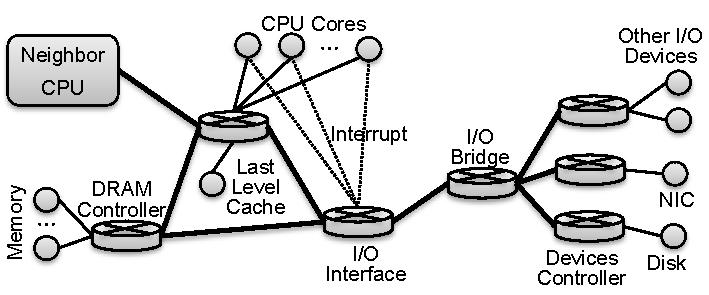
\includegraphics[height=4cm]{intro/computer-as-a-network.pdf}
  \caption[计算机内部本质是一个网络]{
    计算机内部部件之间以数据包(packet)进行通信,比如
    处理器核之间使用基于包的片上网络、
    处理器之间采用基于包的互连协议(如QPI和HT)、
    I/O设备与内存之间则通过PCI-E包进行通信。
    因此,计算机本身即可视为一个网络。}
  \label{fig:computer-as-a-network}
\end{figure}

基于以上需求,
本文提出了一种新体系结构:资源按需管理可编程的体系结构PARD\cite{pard:2015},
使数据中心服务器能够支持区分化服务,通过细粒度的硬件资源管理以及灵活的编程接口,
实现在保障关键应用服务质量的前提下提高服务器资源利用率。
PARD体系结构的核心是基于一个重要的观察:\textbf{计算机内部本质上是一个网络}。
如图\ref{fig:computer-as-a-network}所示,
CPU核、共享缓存、内存控制器、I/O设备等可以被看做是网络节点,它们之间通过包进行通信;
除了处理请求以外,这些``网络节点''与网络中的路由器/交换机具有相似的请求转发功能。
在网络领域,如何实现端到端的服务质量保障已有大量的研究,并已形成标准。
如IETF(Internet Engineering Task Force, 互联网工程任务组)于1998年提出了区分化服务
(Differentiated Services)\cite{DiffServ}的概念,
如今区分化服务已经成为应用最广泛的服务质量保障机制之一;
软件定义网络(SDN)\cite{SDN}的出现,进一步促进了网络领域服务质量保障的发展,其提出的
(1)控制平面与数据平面分离,和(2)集中控制的统一编程接口,
为网络管理带来了极大的灵活性。
本文希望能够将网络领域的区分化服务和软件定义网络的思想应用到计算机内部的网络,
用以解决数据中心当前面临的资源利用率与应用服务质量矛盾。

然而相比在计算机网络,
在体系结构这一``内部网络''中实现区分化服务与软件定义网络的功能需要面临一些额外的挑战:

首先,网络栈是整个网络中产生数据包的唯一位置,因此可以很容易的在其中增加标签机制,
实现网络流的区分。
而在计算机中有大量不同类型的硬件部件都能够向``内部网络''发送请求,
而且这些请求的类型各不相同,
如何为这些来自于不同硬件部件、类型各异的请求增加应用标签是需要解决的第一个挑战。

其次,与网络中交换机或路由器这些只进行存储转发的网络设备不同,
计算机内各个硬件部件通常包含更为复杂的功能,
如:处理器末级缓存需要为请求除完成将请求转发到下层内存控制器外,
还需要决定哪些请求数据缓存在本地,以及替换哪些数据到内存控制器;
内存控制器需要进行复杂的地址映射实现将物理地址映射到DRAM芯片,
同时还需要实现调度策略以提高访存性能;其他一些I/O设备具有更为复杂的功能。
因此如何为这些不同类型的硬件部分提供一个统一的控制平面实现对硬件资源的管理是第二个挑战。

最后,在交换机或路由器中已经为管理员提供了访问和配置其控制平面的固件接口,
而在当前的计算机中并没有类似的的固件接口。
服务器中普遍配置的IPMI/BMC\cite{ipmi}提供了诸如温度监控、电源控制、
BIOS访问等有限的监控与管理功能,利用该模块
如何实现硬件控制平面的管理,以及如何为用户(管理员)提供灵活的访问与编程接口是面临的第三个挑战。

为了解决以上三个挑战,PARD体系结构的核心设计理念可以归结为以下四点:
\textbf{1)标签机制},
通过在请求源(如处理器核或具有DMA功能的I/O设备)增加标签寄存器,使用其记录当前正在使用该部件的应用标签,
发出请求时附带该标签,并随着请求在整个计算机内部传播,实现应用区分;
\textbf{2)可编程控制平面},
为共享硬件资源的控制器增加控制平面,控制平面可根据请求标签查询规则进行区分处理,该规则可通过软件实现可编程;
\textbf{3)节点内统一资源管理},
节点内所有的控制平面通过控制平面网络连接到资源管理模块,提供对控制平面的编程接口,实现所有共享资源的统一管理;
\textbf{4)Trigger$\Rightarrow$Action编程方法},
一种基于动作触发的资源管理策略,实现资源实时监控和调整。

本文后续章节将讨论如何在现有体系结构上扩展以实现标签机制;
通用控制平面的设计以及可编程机制的实现,
并包括末级缓存控制器和内存控制器中控制平面的具体设计;
基于以上两种机制实现无Hypervisor的全硬件支持虚拟化系统,
以及如何实现资源按需分配的区分化服务,并使用模拟器对其效果进行验证。
最后在基于FPGA的原型系统中验证PARD体系结构的效果,
并讨论了原型系统实现过程中的经验与教训。


\section{本文的主要贡献}

本文的论点是:
在应用数量众多、需求多样且不断变化的数据中心场景下,计算机体系结构需要重新设计,
为应用提供区分化服务、良好的性能隔离,并具备灵活的资源管理编程接口,
实现资源使用的强控制与按需分配,
才能解决数据中心资源利用率与服务质量冲突的问题。

本文的主要贡献包括:

% 可在多个层次(虚拟机、进程、线程、API、...)区分应用,实现了NoHyper功能
第一,提出``标签化地址空间(Labeled Address Space)''概念。
正如多进程技术的出现引入了虚拟地址空间抽象,
随着虚拟化、云计算与多租户使用模式的出现,
现有的虚拟地址空间抽象无法满足多租户之间的隔离需求,
一些硬件隔离技术如EPT、I/O MMU、SR-IOV等试图在现有的体系结构下支持隔离需求,
其本质则是在虚拟地址空间外增加一层额外的地址空间,但这些技术只是在功能层面上实现了隔离,
而与性能相关的部件如共享末级缓存、内存控制器等在现有体系结构下并没有实现隔离。
本文提出的标签化地址空间抽象,使用统一标签区分不同应用,
并为计算机系统内所有请求标识应用标签,硬件不再需要通过猜测的方式区分应用,
而是通过标签机制打破目前体系结构中软硬件之间的语言鸿沟,
使得共享的硬件资源能够区分来自不同应用的请求并进行区分处理。
%可在不同层次实现应用区分,如虚拟机、进程、线程或使用API标识的数据/代码段,
%以实现不同粒度的区分化服务。
%以虚拟机粒度为例,通过标签机制以及共享硬件资源内部基于标签的划分机制,
%可将一台计算机划分为多台独立的逻辑域(Logical Domain),
%在每个逻辑域内独立运行操作系统,实现NoHyper\cite{keller_nohype:_2010}的功能。

% 表+Trigger/Action <=> 处理器方案
第二,提出硬件资源共享管理方法,为硬件资源共享提供配置、监控、反馈功能,
实现毫秒(ms)级的性能反馈。
%本文两个重要观点是:资源监控与管理结合,共享资源本地与全局协同管理结合。
实时的监控与反馈是实现细粒度资源管理的重要前提,软件监控方案无法满足实时性的需求,
在硬件上直接实现监控与反馈,提出使用通用的``控制平面''实现硬件资源的配置与监控。
在具体实现上,通过基于表的控制平面实现通用的硬件资源管理接口,
使用基于处理器的数据平面实现硬件请求的灵活控制,
为计算机系统实现硬件资源可管理提供支持。

第三,提出节点内硬件共享资源的协同管理。
控制平面构成了计算机系统内硬件资源管理的基本单元,由于硬件资源之间具有关联性,
需要进行全局统筹管理。
本文通过使用控制面网络将节点内所有的控制平面连接到集中式的资源管理模块,
对硬件共享资源进行协同管理。

以上三点贡献已在PARD的模拟器及FPGA原型系统中实现。
模拟器原型是基于gem5\cite{binkert_gem5_2011}实现的全系统时钟精确模拟器,
增加或修改了大约24,118行C++/Python代码,该模拟器以在LGPL协议下开源
\footnote{PARD-gem5模拟器开源地址https://github.com/fsg-ict/PARD-gem5}。
FPGA原型系统基于MicroBlaze系统在Xilinx VC709开发板实现并完成验证,
系统运行在133MHz频率,包含4个处理器核。
两个原型系统可以作为后续相关研究的参考平台。


\section{论文的组织}

\begin{figure}[htb]
  \centering
  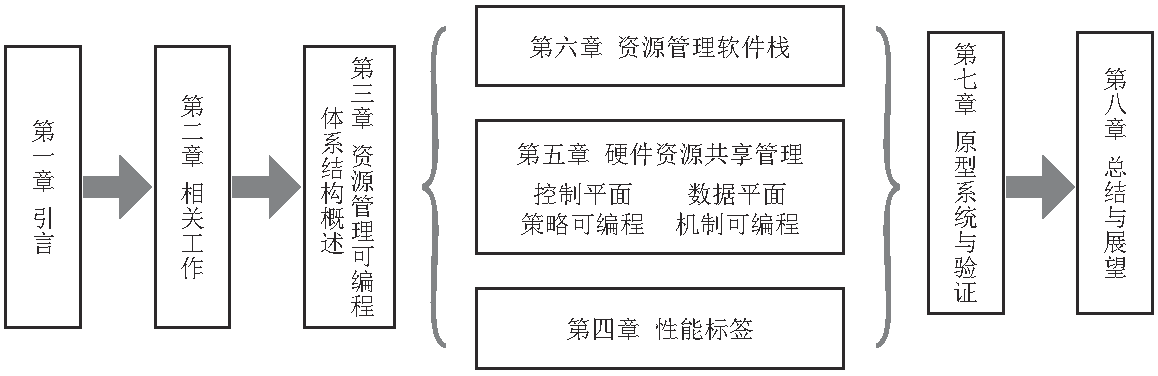
\includegraphics[width=\textwidth]{intro/thesis-structure}
  \caption{本文内容与组织结构}
  \label{fig:thesis-structure}
\end{figure}

本文共分八章,组织结构如图\ref{fig:thesis-structure}所示。

第二章介绍数据中心面临的资源利用率与服务质量冲突问题的挑战,
然后讨论现有数据中心技术的局限性,
并介绍解决该问题的现有研究。

第三章介绍PARD体系结构与关键特性,
并讨论如何利用PARD所提供的特性解决应用服务质量与资源利用率相冲突的问题。

第四章介绍PARD体系结构的基础标签化地址空间,
讨论在现有体系结构下实现标签化地址空间需要解决的关键问题,
并在模拟器上通过标签化地址空间改造,实现无软件支持的全硬件虚拟化功能。

第五章讨论硬件共享资源的管理方法,包括硬件资源的控制平面/数据平面抽象,
同时以共享末级缓存和内存控制器为例,讨论控制平面与数据平面的设计,
并通过模拟的方式验证该方案的有效性。

第六章介绍资源管理模块与资源协同管理相关的内容,包含节点内资源统一管理,
以及如何将PARD集成到现有的数据中心管理系统中(以Mesos\cite{Hindman:2011:Mesos}为例)。

第七章基于前四章的设计给出本文资源管理可编程体系结构的FPGA原型系统实现,
并对原型系统各部分功能的正确性、性能与开销进行评测。

第八章总结全文并介绍未来可能的研究工作。


% 
%%% Local Variables: 
%%% mode: latex
%%% TeX-master: t
%%% End: 

\chapter{相关研究}
\label{chap:related}

互联网应用如电子邮件、搜索、网络购物、社交网络、在线视频、网络地图等, 已经成为人们
生活的一部分。这些应用往往要为上亿用户服务,意味着互联网应用已变成如电力一样的社会
公共服务,而支撑拥有海量用户互联网应用的数据中心也成为如同发电厂一样的社会核心基础
设施。

长尾延迟(Tail Latency)问题在数据中心中受到越来越多的关注,造成长尾延迟的原因有很
多,其中最为重要的原因就是资源共享带来的干扰。
由于没有行之有效的方案对干扰进行控制,目前典型的数据中心都使用隔离的方式来减小干扰,
这一方案虽然有效缓解了长尾延迟,但它也带来了资源利用率过低的问题,
现有商用数据中心的资源利用率普遍只有10\%-30\%左右,造成极大的浪费。
如何解决服务质量与资源利用率的问题是当前业界面临的重大挑战。

本章内容安排如下:首先介绍新计算模式对数据中心的挑战,然后讨论现有数据中心技术的局
限性,即服务质量与资源利率冲突的原因,进而提出一种面向数据中心应用服务质量保障的
体系结构,最后将阐述本文的研究动机,介绍本文的主要贡献和组织结构。

%服务质量(QoS)与资源利用率是数据中心运营时需要考虑的两个重要指标,前者严重影响用户
%体验,而后者直接与数据中心的运营成本相关。然而现有的计算机体系结构并没有为服务质量
%保障提供足够的支持,造成这两个指标在现实状况下存在冲突。为了保障用户体验,在实际系
%统部署时,会更多的考虑服务质量这一指标,造成数据中心的资源利用率严重低下,普遍只有
%10\%-30\%左右。基于这一现状,本文主要讨论如何设计一种高效的数据中心体系结构,使得
%数据中心在保障应用服务质量基础上,达到较高的资源利用率。
%

\section{新计算模式对数据中心的挑战}

\subsection*{计算模式1:以云计算为基础的移动计算}

随着移动设备(平板电脑、智能手机)计算能力不断增强、成本不断降低以及无线通信技术的
快速发展,移动计算时代已经来临。如表\ref{tab:ganter-sales}所示,
Gartner调研数据显示平板电脑和手机(包含智能手机和普通手机)销量不断增加,
与此同时PC销量则不断下降。
而IDC预测到2015年智能手机销量将超过14亿部,占所有个人计算设备(包括PC、平板电脑和智能手机等)69\%的销量份额。

% Gartner关于电脑与移动设备销量的统计 
\begin{table}[htb]
  \centering
  \begin{minipage}[t]{0.9\linewidth}
  \caption[全球个人计算设备市场销量统计]{全球个人计算设备市场销量统计(单位:千部)}
  \label{tab:ganter-sales}
    \begin{tabular*}{\linewidth}{lrrrrr}
      \toprule[1.5pt]
      {\heiti 设备类型} & {\heiti 2012年} & {\heiti 2013年} & {\heiti 2014年} & {\heiti 2015年} & {\heiti 2016年} \\
      \midrule[1pt]
      PC(台式机、笔记本) &   341,273 &   296,131 &   279,000 &   259,000 &   248,000 \\ 
      超级本               &     9,787 &    21,517 &    39,000 &    62,000 &    85,000 \\ 
      平板电脑             &   120,203 &   206,807 &   216,000 &   233,000 &   259,000 \\ 
      手机                 & 1,746,177 & 1,806,964 & 1,838,000 & 1,906,000 & 1,969,000 \\ 
      其它移动设备         &       --- &     2,981 &     6,000 &     9,000 &    11,000 \\
      %总计                 & 2,217,440 & 2,334,400 & 2,378,000 & 2,470,000 & 2,572,000 \\
      \bottomrule[1.5pt]
    \end{tabular*}\\[2pt]
    \footnotesize
    数据来源:Gartner,2012年(http://www.gartner.com/newsroom/id/2610015),
    2013年(http://www.gartner.com-\\/newsroom/id/2791017),
    2014-2016年(http://www.gartner.com/newsroom/id/2954317)
  \end{minipage}
\end{table}

移动计算的快速发展带来新的计算模式:移动设备通过无线通信与运行在云计算平台的各类应
用服务进行交互。据可靠消息,目前一些主要的互联网公司(如Facebook和Baidu等)均表示,
来自移动设备的请求已占到40\%以上,并且仍在快速增长,很快将超过PC。随着4G时代的到来,
这种移动计算模式将成为未来的主流。

快速增长的移动计算需求对云计算平台的核心——数据中心带来了严峻的挑战。这种交互式计算
模式,快速的服务响应时间是衡量服务质量(Quality-of-Service,QoS)的关键指标,是让用
户满意、留住用户的关键。有研究表明,如果服务响应时间增加,公司收入就会减少。
例如,2009年微软在Bing搜索引擎上也开展实验,发现当服务响应时间增加到2000ms时,
每个用户带给企业的收益更是下降了4.3\%。由于该实验对公司产生了负面影响,最终不得不被
终止[8]。Amazon也发现其主页加载时间每增加100ms就会导致销售额下降1\% 。而Google更是
发现当搜索结果返回时间从0.4s增加到0.9s时,广告收入下降了20\%。

\begin{figure}
\begin{minipage}{0.48\textwidth}
  \centering
  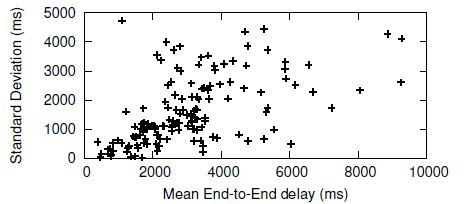
\includegraphics[height=5cm]{intro/end2end-delay}
  \caption[北美移动应用用户感知时延分布]{北美移动应用用户感知时延分布:平均延迟超过2秒且具有很大的波动性}
  \label{fig:end2end-delay}
\end{minipage}\hfill
\begin{minipage}{0.48\textwidth}
  \centering
  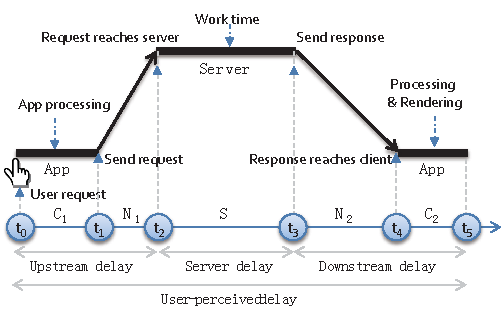
\includegraphics[height=5cm]{intro/interact-apps}
  \caption[一个典型的交互式请求的5个阶段]{一个典型的交互式请求的5个阶段:C1->N1->S->N2->C2 \cite{timecard2013}}
  \label{fig:interact-apps}
\end{minipage}
\end{figure}

移动计算的响应时间仍然存在很大的提升空间。
如图\ref{fig:end2end-delay}所示,微软公司实验数据表明在北美网络环境下,
交互式移动设备的平均时延超过2秒,而且存在较大的波动性。
图\ref{fig:interact-apps}显示典型移动交互式应用的用户请求时延分为5个阶段,
最近研究\cite{timecard2013}表明其中数据中心服务器的处理时延S约为1.2秒,占60\%。
随着4G网络的来临,数据中心将面临更大规模用户数据的处理请求。
因此,如何快速处理和及时响应移动计算请求将成为数据中心设计的核心目标之一。


\subsection*{计算模式2:面向大数据处理的实时计算}

大数据时代的到来使大数据处理架构受到越来越多的关注。2013年底中国计算机学会(CCF)
大数据专家委员会发布的《2014年大数据发展趋势十大预测》 报告中,来自学术界、产业界、
海外、跨界特邀和政府的122位专家们普遍认为,Hadoop/MapReduce框架一统天下的模式将被
打破,而实时流计算、分布式内存计算、图计算框架等将并存。

\begin{figure}[H]
  \centering
  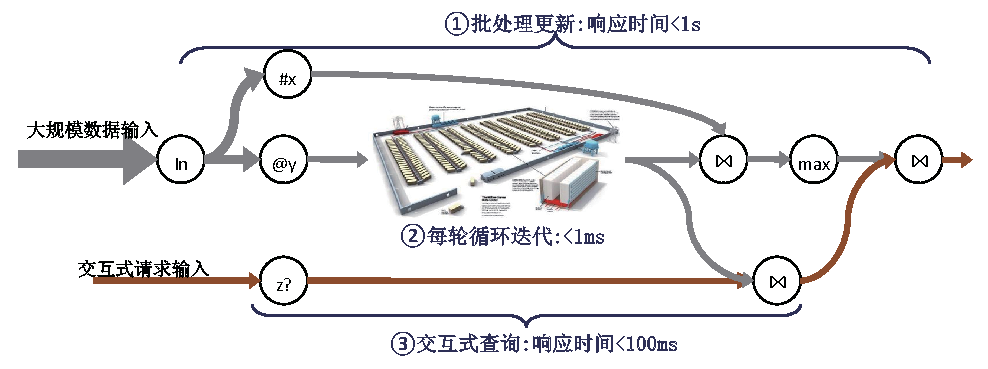
\includegraphics[height=6cm]{intro/batch-apps}
  \caption{典型的3类大数据处理需求以及相应的响应时间要求}
  \label{fig:batch-apps}
\end{figure}


大数据处理对数据中心和处理架构提出新的挑战,图\ref{fig:batch-apps}显示了典型的
大数据处理需求:首先需要支持数据的批处理更新模式(<1s);
其次数据处理会分解为多次迭代计算(<1ms);
再次还要支持实时计算模式,处理多用户的交互式查询请求(<100ms);
而这些处理所需要的数据
存放在同一个数据中心。搜索引擎是一个典型的例子,既需要对大规模网页进行内容处理,
迭代计算页面的pagerank,还需要处理大量用户的关键字查询请求。

尽管大数据处理希望能将各种处理集成在一个处理架构上,然后部署在一个数据中心。但如果
实时计算与企业营收相关,比如搜索引擎、在线购物等在线服务应用,那么正如微软Bing实验
所示,这些面向在线服务应用的实时计算的服务质量就非常关键(以下用“在线应用”
代表“实时计算”)。为了保障在线应用的服务质量,主流互联网企业一般将在线应用与大规模
批处理作业分别部署到不同的数据中心,以减少批处理作业对在线应用的干扰。但由于用户查
询请求数量具有显著的随时间变化的波动性,这种分离作业、单独部署的模式会导致在线应用
数据中心的资源平均利用率很低。如图4所示,Google的两类数据中心CPU利用率相差达2.5倍,
在线应用数据中心资源利用率仍有很大提升空间。


%% 典型的数据中心一般有5~10万台服务器组成,建设与运行维护成本往往高达几十亿人民
%% 币。然而出于保障应用服务质量的原因,现有数据中心只能维持较低的资源利用率,导致大量
%% 资源浪费。因此,本项目总体研究目标为如何设计高效通用数据中心体系结构:“通用”表
%% 示数据中心可同时运行各种不同类型应用;“高效”表示数据中心能在保障延迟敏感应用的服
%% 务质量基础上,达到较高的资源利用率(CPU利用率>60\%)。
%% 
%% 典型的数据中心一般有5~10万台中低端服务器组成,这些服务器通过内部网络互连,一起协同
%% 运行互联网应用为海量用户服务。因为这类数据中心规模很大,往往部署在大型仓库级别的机
%% 房,从应用角度来看就如同一台计算机,因此也被称为
%% “仓库级计算机(Warehouse-Scale Computer)“ \cite{WSC}。
%% 国内外著名的互联网公司往往拥有多个数据中心,服务器数量达到数十万甚
%% 至上百万台。例如,谷歌(Google)的数据中心服务器数量已经超过百万台为全球用户提供
%% 搜索、邮件、地图等服务[2];亚马逊(Amazon)仅EC2就部署了约50万台服务器提供云计算服
%% 务[3];据可靠消息,国内腾讯公司也拥有约30万服务器为用户提供各种互联网服务。
%% 
%% 尽管目前互联网企业的数据中心已经颇具规模,但一个趋势是未来数据中心还将持续发展。一
%% 方面互联网用户数量仍在不断增长,目前全球已有24亿网络用户,但很多机构预测未来全球还
%% 将新增30亿网民融入到互联网[4],这会对数据中心的数量和规模都提出更多需求。另一方面快
%% 速发展的移动终端已超越个人计算机(PC),成为终端计算设备的主流。由于移动设备性能相对
%% 较低、存储容量较小,将计算与存储转移到数据中心的需求也变得越来越强烈。因此数据中心作
%% 为基础设施也会日益重要。


\section{现有数据中心技术的局限性}

通过上述分析可知,移动计算与实时计算均对快速响应用户请求提出了强烈的需求。而当前数
据中心为了保障用户请求的服务质量,不得不通过采用牺牲资源利用率、保留过量资源的方式。
Google的数据中心技术一直处于领先地位,我们以Google为例分析数据中心资源利用率现状。
图\ref{fig:google-util-2006}显示了2006年Google数据中心平均CPU利用率为30\%左右。
但到2013年,虽然Google将数据中心分为了两类,并且批处理数据中心已经能达到75\%的CPU利用率,
但在线应用数据中心仍停留在30\%。
我们对国内企业调研发现,几大主流互联网企业在线应用数据中心CPU利用率一般都低于20\%,
有的甚至低于10\%,仍然存在很大的提升空间。

% Google数据中心利用率 
\begin{figure}
\begin{minipage}{0.57\textwidth}
  \centering
  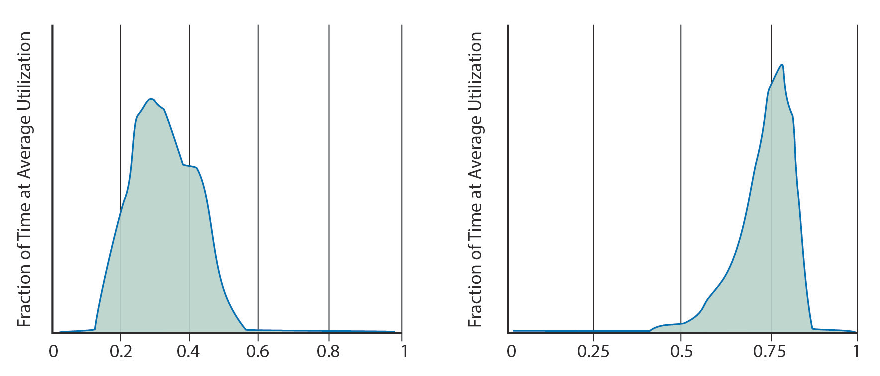
\includegraphics[height=4cm]{intro/google-util-2013}
  \caption[Google数据中心CPU利用率分布(2013年)]
    {Google数据显示2013年1至3月在线应用数据中心CPU利用率平均只有30\%(左图),
     而批处理作业数据中心则能达到75\%的利用率(两个数据中心均为2万台服务器)}
  \label{fig:google-util-2013}
\end{minipage}\hfill
\begin{minipage}{0.39\textwidth}
  \centering
  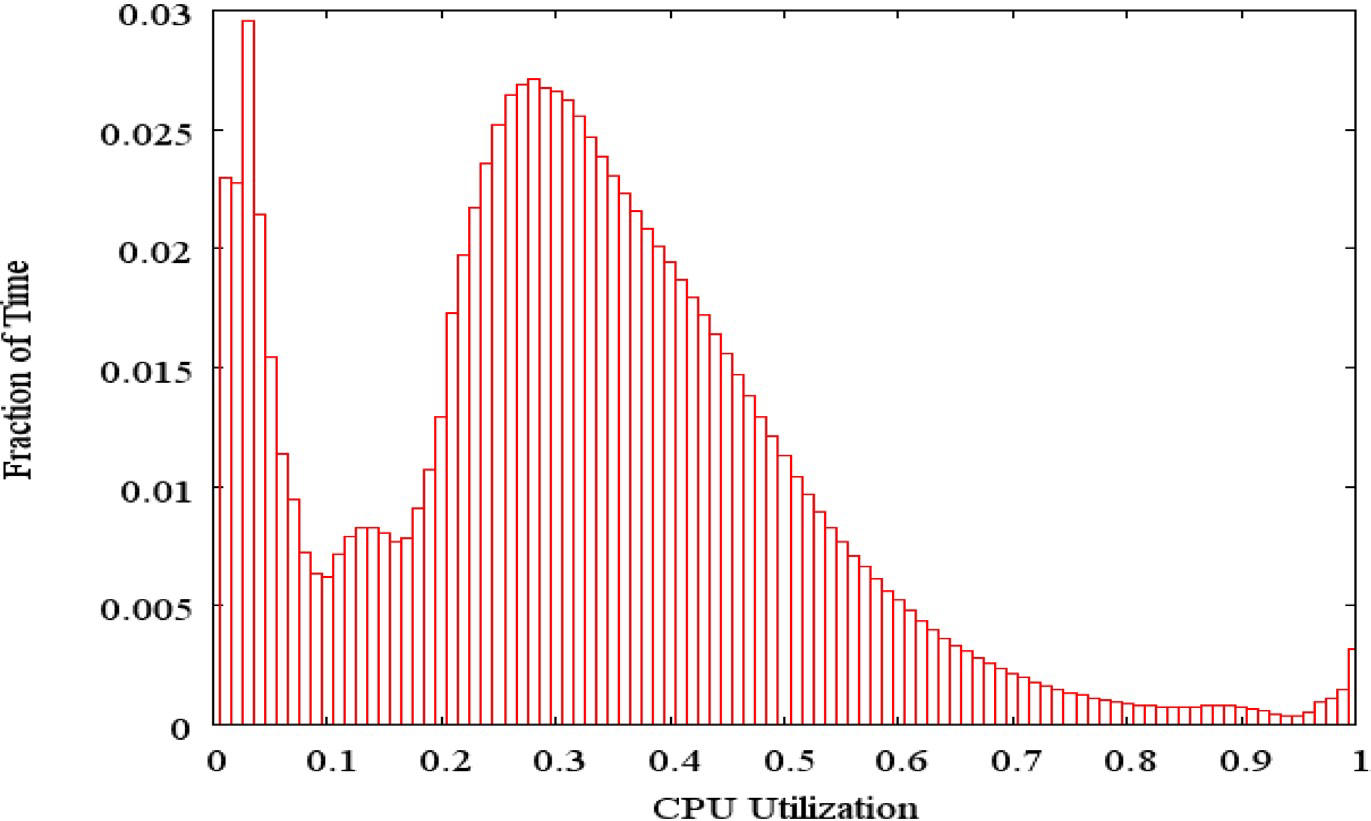
\includegraphics[height=3.5cm]{intro/google-util-2006}
  \caption[Google数据中心CPU利用率分布(2006年)]
    {Google在2006年数据中心(5000台服务器)6个月的CPU利用率分布}
  \label{fig:google-util-2006}
\end{minipage}
\end{figure}

尽管在线数据中心资源利用率只有30\%,但Google已经观察到严峻的长尾延迟现象---最慢的
1\%~10\%请求处理时间远大于所有请求的平均响应时间。
如图6所示,Google某后台服务延迟响应时间平均仅为5~6ms,但是却有相当一部分请求响应时间
超过了100ms[49]。而长尾延迟现象在数据中心环境下会被更进一步放大,因为一个用户请求需要
几百上千台服务器共同完成,只要有一台服务器的处理速度受到干扰,就会导致整个请求的处理
时间增加。Google的Jeff Dean在2012年Berkeley的报告[11]中就指出了长尾现象的严重性,假设
一台机器处理请求的平均响应时间为1ms,有1\%的请求为长尾处理时间会大于1s 
(99th-Percentile)。如果一个请求需要由100个这样的节点一起处理,那么就会出现63\%的请求
响应时间大于1s(如图7所示)。

造成在线应用数据中心资源利用率低和长尾延迟现象的核心原因是现有数据中心技术无法在多
应用混合运行时消除应用间干扰,以实现不同应用之间的性能隔离。
Google的Jeff Dean与Luiz Barroso在2013年2月的《Communication of the ACM》上撰文
“The Tail at Scale”[10]分析确认导致长尾延迟的首要原因就是资源共享,
包括体系结构层次的CPU核、Cache、访存带宽、网络带宽等,而干扰不仅来自应用,
还会来自系统软件层次的后台守护作业、监控作业、共享文件系统等。
Google在分布式架构和软件层次采用了多种缓解长尾延迟的技术,
包括操作系统容器隔离技术[12]、应用优先级管理[13]、备份请求[11]、同步后台管理进程[11]等,
取得了一定的效果,但却无法消除硬件体系结构层次上的应用之间的干扰,
导致仍然会出现图6这样的长尾延迟。

因此,现有数据中心处于“无管理的资源共享”状态,这
导致出现资源利用率与应用服务质量之间的矛盾:
一方面通过多个应用同时在数据中心部署实现资源共享能有效提高资源利用率,
但另一方面多个应用共享资源又会出现相互干扰严重影响应用的服务质量。
因此,目前企业不得不采用预留额外资源以保障延迟敏感的在线应用服务质量,
这导致很低的数据中心利用率。
而且随着多核技术的发展,单个服务器内的资源越来越多,
其上混合部署的应用数目也在不断增加,更会加剧这种矛盾。


\section{本文的研究动机}

现有数据中心技术面临资源利用率与应用服务质量的矛盾,其根本原因是大量数据中心共享资源
属于“无管理共享”状态。要实现高效通用数据中心目标,核心是从硬件上改变资源的“无
管理共享”现状以实现在体系结构上支持应用服务质量保障,在此基础上实现数据中心资源根据应
用动态管理以提高资源利用率。

回顾历史,当前数据中心面临的问题与1990年代的Internet具有相似之处。
当时流媒体、电子商务、电子邮件和FTP等大量网络应用的兴起,它们具有不同的QoS需求。
为了在IP网络中为这些应用提供端到端的服务质量保障,
互联网工程任务组(Internet Engineering Task Force, IETF)于1998年提出了区分化服务
(Differentiated Services)的概念。而如今,区分化服务已经成为应用最广泛的服务质量保障
机制之一。该技术的核心是在IP包头中定义长度为8-bit的区分化服务域,用以表示应用的
服务质量分类标识,因此路由器、交换机等网络设备便可以使用该信息对不同类别的数据包
进行区分处理,以达到区分化服务的目的。
软件定义网络(SDN)的出现,进一步促进了网络领域服务质量保障的发展,
其主要原理可以概括为:(1) 控制平面与数据平面分离;(2)集中控制的统一编程接口。

同时,计算机内部也可以被看做一个网络,如图\ref{fig:computer-as-a-network}所示,
CPU核、共享缓存、内存控制器、I/O设备等可以被看做是网络节点;除了处理请求以外,
这些“网络节点”与网络中的路由器/交换机具有相似的请求转发功能;
而它们之间也通过包进行通信,如:片内通信使用NoC包,片间通信的QPI/HT包,
以及I/O部分使用的PCI-E包。
将网络领域的区分化服务和软件定义网络的思想应用到计算机内部的网络,
用以解决数据中心当前面临的资源利用率与应用服务质量矛盾,是本文的主要研究思路与动机。

与在网络中部署SDN相比,在计算机体系结构“网络”中部署SDN会面临以下三个挑战:

首先,在整个网络栈中EndPoint是唯一的请求来源,因此SDN可以很容易的将标签机制实现在网络栈中;
与之相对的,在计算机体系结构中存在大量的硬件部件都能够发送请求,而这些请求类型又不尽相同,
因此在这样的环境下如何为请求打上标签是一个很大的挑战。

其次,在网络中所有的交换机都执行相同的存储/转发(store-and-forward)操作,但在计算机内部
不同的部件都有不同的功能,而不只是简单的存储/转发,如何为这些不同类型的部件(如末级缓存控制器、
内存控制器、I/O设备等)设计统一的控制面结构是另一个挑战。

最后,在网络交换机中已经包含了一个firmware固件用于访问和配置交换机的控制面,但计算机中却缺少
这样的firmware。现有的IPMI只被用来做有限的监控与管理功能,如对温度、风扇转速和电源控制。
因此,需要在计算机内部提供一种这样的部件实现与其它众多的控制面的通信与管理,并提供一个灵活的
编程接口对这些控制面进行操作。


%本项目总体研究目标是研究新型高效通用数据中心体系结构,能在保障应用服务质量
%的基础上将数据中心计算资源利用率提高到60\%以上。从技术挑战来看,计算机资源管理亟需新的
%具有以下特征的技术架构:
%(1)细粒度共享,有利于提高资源利用率;
%(2)性能隔离,有利于提高应用服务质量;
%(3)快速动态响应,有利于资源按需分配;
%(4)灵活协同配置,有利于协同多种资源配置以适应多种应用场景。


\section{论文的主要工作}

%本研究的目的是通过对真实环境、真实应用的访存行为特征进行更全面细致的分
%析,
%探索服务质量保障的体系结构支持,
%内存系统影响计算机整体性能的更深层次的原因,从而为体系结构、系统软件
%等的设计与优化提供一些建议。

%\begin{description}
% \item[First] \hfill \\
% The first item
% \item[Second] \hfill \\
% The second item
% \item[Third] \hfill \\
% The third etc \ldots
%\end{description}


本研究的目的是在体系结构层次解决数据中心所面临的资源利用率与服务质量相冲突的问题,
论文的主要工作围绕下述三个阶段开展:

\begin{itemize}
 \item 本研究在Xeon E5-v3平台上验证Cache容量划分功能对应用性能隔离带来的作用,
       并提出一种基于反馈模型的缓存自适应分配方法。
 \item 在体系结构内引入标签,实现应用区分,并在各个共享资源对其进行区分处理
 \item 提出一种资源管理可编程体系结构,实现可编程的硬件共享资源的细粒度管理
\end{itemize}


\section{论文的主要贡献}
In this paper, we propose Programmable Architecture for
Resourcing-on-Demand (PARD) that provides a new programming
interface to convey an application’s QoS requirements to the hardware.
PARD supports new functionalities such as fully hardwaresupported
virtualization without software hypervisors and differentiated
service (DiffServ) [60] in data center servers. For instance,
PARD can accurately isolate performance in shared data centers
to improve server utilization without degrading QoS for latencycritical
applications.



\section{论文的组织结构}

本文共分八章,第一章介绍移动计算带来的新计算模式对数据中心的挑战,然后讨论现有
数据中心技术的局限性,并针对现有体系结构提出了新的需求,最后介绍了论文的研究动机、
主要贡献和组织结构。

第二章介绍体系结构领域解决服务质量问题的现有研究,并对比以网络领域的相关内容,
讨论两者相互借鉴的可能性。

第三章对现有体系结构的服务质量支持进行评估,包括软件(cgroup, hyperviso)和硬件
两个层次。

第四章介绍资源管理可编程体系结构的概念与核心思路,并将其映射到现有体系结构,
讨论其可行性。同时应用资源管理可编程体系结构实现全硬件虚拟化,并讨论其关键技术。

第五章讨论模拟器实现,主要从功能设计角度对控制面设计,与资源管理可编程实现,
硬件支持、Trigger-Action机制,模拟的方式验证PARD的有效性。

第六章基于前两章的设计给出本文资源管理可编程体系结构的FPGA原型系统实现,
并对原型系统各部分功能的正确性、性能与开销进行了详细评测。

第七章在数据中心场景下,对本文资源管理可编程体系结构在分布式场景下应用进行讨论。

第八章总结全文并介绍未来可能的研究工作。


处理应用服务质量与资源利用率的问题,在互联网公司、芯片厂商还是学术界都在想办法解决
该问题:互联网公司方面,Baidu的Matrix项目、Google的Borg和Omega、Facebook的mesos系统
都尝试在软件架构层面解决该问题;Intel最新发布的Xeon E5-v3系列芯片,ARM芯片等都对QoS
提供了一定的支持;学术界在软硬件调度、划分方向也有大量工作。但这一问题并没有被解决,
本章首先介绍数据中心应用及其服务质量评价指标,并对现有工作进行总结,并分析其局限性。
同时参考网络领域在解决该问题的方案,

实现高效通用数据中心目标的前提在于保障应用服务质量。类似于系统安全需要所有环节安全
才能保障端到端(End-to-End)的安全,服务质量保障也需要应用全生命周期所有环节的支持。
在数据中心层面,这需要从服务器节点内部、服务器之间通信以及分布式架构多个层次协同工作。
近年来,学术界、工业界在这三个层次都不断努力。例如,近年来流行的Software Defined
Networking(SDN)技术\cite{SDN}目标就是解决数据中心网络通信的管理、共享与性能隔离问题。
Google在分布式架构上采用了超时发送备份请求同步后台管理进程等技术[11]来提高服务质量。
单节点内服务质量保障技术已成为短板。由于体系结构上不支持服务质量保障,而主流的软件
隔离技术能对资源容量隔离起到较好的效果,但无法保障性能隔离,无法保障服务质量。
总的来说,国内外在保障应用服务质量方面的研究包括单节点与分布式环境两个方面。
以下分别从这两个方面介绍相关工作。


应用混合的目标分为两方面:一是提高资源利用率,二是保障关键应用的服务质量。现有的运行时
管理方案[15]–[17]大都通过硬件性能计数器对关键应用的性能进行监控,并在性能发生下降时对非
关键应用进行各种处理,以减小由于资源竞争引起的性能问题。

造成资源利用率的核心问题在于计算机资源处于“无管理共享”状态,因此多个应用共享资源时会发
生竞争与干扰,最终导致关键应用性能不可预测。目前尚无很好的技术方案解决计算机资源“无管理
共享”的问题,以Google为代表的工业界采用将在线服务器与离线服务器分离的方法,通过降低在线
服务器的负载来保障在线应用的服务质量。

学术界在共享资源管理方面从2个维度、4个方面开展研究:软件调度、软件划分、硬件调度、硬件
划分。软件调度是通过操作系统/Hypervisor层次进行进程、线程或虚拟机级别的调度,一般调度粒
度较大,需要上下文切换,时间上也需要几毫秒到几十毫秒,不能满足在线应用的快时响应的需求;
软件划分技术能对Cache容量进行划分,但无法管理访存带宽这类资源,且软件划分技术配置调整开
销较大;硬件调度技术能支持访存请求级别的细粒度调度,但灵活性较多,不能根据不同应用按需管
理;硬件划分技术对Cache容量比较有效,但也无法对带宽等进行管理,而且同样面临灵活性差的问
题。面对诸多问题,斯坦福大学Christos Kozyrakis教授提出应该重新考虑整个计算机架构,从应用
特征、硬件隔离、操作系统、机群调度、高效资源管理硬件等多层次协同设计[18]。

\section{调度方法}
\label{sec:other}

实现高效通用数据中心目标的前提在于保障应用服务质量。类似于系统安全需要所有环节安全才能保障端到端(End-to-End)的安全,服务质量保障也需要应用全生命周期所有环节的支持。在数据中心层面,这需要从服务器节点内部、服务器之间通信以及分布式架构多个层次协同工作。近年来,学术界、工业界在这三个层次都不断努力。例如,近年来流行的Software Defined Networking(SDN)技术[15]目标就是解决数据中心网络通信的管理、共享与性能隔离问题。Google在分布式架构上采用了超时发送备份请求同步后台管理进程等技术[11]来提高服务质量。单节点内服务质量保障技术已成为短板。由于体系结构上不支持服务质量保障,而主流的软件隔离技术能对资源容量隔离起到较好的效果,但无法保障性能隔离,无法保障服务质量。

总的来说,国内外在保障应用服务质量方面的研究包括单节点与分布式环境两个方面。以下分别从这两个方面介绍相关工作。

1.2.1 单机保障服务质量研究

单机保障服务质量相关研究包括软件资源隔离技术、软硬件调度技术、硬件支持等。

软件隔离技术:针对数据中心里多个应用相互干扰的问题,一般采取虚拟化的手段在资源共享的条件下保障资源隔离,如虚拟机技术Xen[18]或Linux Container[17]。

传统虚拟机技术通过将多台虚拟机VM部署到物理机上,每台虚拟机运行一个应用或应用的一个组件,每个应用在自己的操作系统环境中独立运行,减少相互之间干扰。但这些隔离主要是资源的隔离,而无法实现性能隔离。例如为不同应用分配不同的访存带宽。而且使用虚拟机也会带来一定的性能损失[20],增加延迟,带来性能波动。

Linux Container[17]是一种轻量级虚拟化,通过在操作系统层面增添虚拟服务器功能,操作系统内核能够提供多个互相独立的用户态实例。每个用户态实例对于它自己的用户来说都像是一台独立的计算机,有自己独立的网络、文件系统、库函数和系统设置等。操作系统级虚拟化技术的优点是性能开销较小,不需要硬件的特别支持,而且能为用户态实例之间提供一定的隔离性,所以被广泛地应用在虚拟主机服务器环境中。然而,容器虚拟化技术的虚拟对象不是实际的物理资源(处理器、内存和外设),而是从用户角度出发而抽象的操作系统内部资源资,如CPU时间,内存,I/O带宽等,但如图1.5所示,Container技术对性能隔离效果并不理想。事实上,在性能隔离方面也有相关研究, Rice大学的Druschel等人[21]设计了Resource Container系统, 实现了单台物理机上多个应用间的性能隔离和CPU细粒度资源分配机制支持,然而局部隔离并不能保证全局隔离,Druschel 等人又设计了Cluster Container系统[22],以解决应用在集群范围内的隔离问题。但十几年前,单机核数目非常小,如今单节点已经有几十个核,同时运行的应用也增加了一个数量级,出现了很多新的挑战。

页着色(Page Coloring)[33]是一种以软件方式控制内存物理页映射到处理器缓存上的技术,映射到同一缓存块中的物理页对应同一颜色。基于页着色技术可以实现对共享二级缓存的划分(Partition)[36],能缓解应用在共享二级缓存上的干扰。Cho等人[34]使用Page Coloring技术来管理共享缓存。Tam等人[35]在Linux内核上实现了基于页面着色的缓存划分策略。而对于DRAM系统,也可以使用页着色技术对共享DRAM颗粒进行划分[37][39],例如,Liu等人[40]在Linux内核上实现了基于页着色的DRAM颗粒划分。北京大学李晓明教授团队也在这方面做了很多工作[41][42][43],研究利用页着色技术在虚拟环境下对共享Cache进行了划分。页着色技术能缓解一些粗粒度共享资源层次的干扰,但无法解决微体系结构的干扰,比如共享队列等,并且使用不灵活。总结而言,软件隔离技术能对资源容量隔离起到较好的效果,但无法保障性能隔离,无法保障服务质量。

软硬件调度:在多核微体系结构上,由于共享片上和片外资源的竞争会引起跨核应用之间的干扰。Jason Mars和Neil Vachharajani等人提出了竞争感知的轻量级运行时环境CAER[25],能在提高利用率的同时减少由竞争引起的跨核干扰问题。他还和Lingjia Tang等人在文章[24]还介绍了CiPE框架,可以直接用于测量和量化多核结构下应用的跨核干扰敏感度。Jason Mars等人还设计了Bubble-Up[23]机制,通过使用气泡(Bubble)来代表内存子系统的可变压力情况,能准确预测在内存子系统中竞争共享资源而导致的性能下降。Lingjia Tang等人在文章[29]提出了一种动静结合的编译方法ReQos,在确保高优先级应用的服务质量的同时让低优先级应用也可以自适应地执行。ReQoS包含一种由配置文件引导的编译技术,来识别低优先级应用中有争议的代码段。这些调度相关的工作,在具有大规模真实应用的Google“混布”数据中心里,使用该机制能在保证延迟敏感性应用的服务质量的同时,能显著提高50%~90%的资源利用率。但这些工作属于Ad-hoc类型,针对特定场景有效,并没有从根本上解决问题。

以CMU的Onur Mutlu为代表的一些学术界专家在提出了一系列调度算法[44][45][46]以缓解内存控制器的不公平问题,从而提高系统吞吐量以及服务质量。但这些算法是固化的,并不能针对某个应用进行调节,不具有灵活性。

体系结构支持:Ravi Iyer在文章[30]中提出了一种保障CMP体系结构上缓存Qos的管理框架,设计了CQos优先级分类、优先级分配和优先级执行。CQos优先级分类和优先级分配采用的是从用户到开发人员驱动的编译检测和基于流的方法;CQos优先级执行则包括(1)选择高速缓存分配、(2)动静态结合设置分区、(3)异构缓存区域。实验结果表明, CQoS在多线程或多核平台上能提高共享缓存的效率和系统性能。然而,文章[30]并没有详细描述保障CMP体系结构上缓存Qos的具体策略和软硬件支持。所以,Ravi Iyer等人又在文章[31]中实现了一种在CMP平台上保障Qos的内存体系结构,允运行时的动态资源再分配,能在减少低优先级应用性能下降的同时优化高优先级应用的性能。Andrew Herdrich等人[32]证明了用于功耗管理的基于速率(rate-based)的技术能适应于CMP结构上缓存/内存的Qos管理,其基本方法是当正在运行的低优先级任务由于资源争用而干扰了高优先级任务的性能时,就减缓核心的处理速率。通过评估时钟调制和频率缩放这两个速率限制机制,发现时钟调制更适用于缓存/内存Qos管理。

Ravi Iyer在体系结构支持服务质量方面做了一些有价值的工作,但主要集中在内存方面,并没有从整个系统角度去考虑。事实上,我们认为这个方向在未来会越来越重要,值得深入研究。
 
1.2.2 分布式环境保障服务质量

在分布式环境下,影响应用服务质量的因素主要是节点故障与干扰引起的长尾延迟,下面将从这两个方面介绍相关优化技术。

软硬件故障:Jean Dean等人设计MapReduce[26]的初衷是使用由成百上千机器组成的集群来处理超大规模的数据,所以,要求必须MapReduce能很好地处理机器故障。MapReduce采用了任务重新调度或重新执行任务(backup task)的方法来解决节点故障或短暂忙碌。比如,如果一个机器的硬盘出了问题,读取数据的速度从30M/s降低到1M/s, MapReduce框架中发送backup task机制来减少这一类长尾延迟。Backup task机制通常只会占用比正常操作多几个百分点的计算资源,但能显著改善因为故障出现的长尾延迟。不过,类似于TCP重传机制,backup task的有效性会随着负载的提高而削弱。


竞争共享资源引起的干扰:为了缓解干扰引起的长尾延迟现象,Dean等人[10]介绍了Google采用的缓解长尾延迟的技术,包括操作系统容器隔离技术[12]、应用优先级管理[13]、备份请求[11]、同步后台管理进程[11]等。R. Kapoor等人在文章[27]中提出了Chronos架构,以降低数据中心应用的长尾延迟。Chronos基于NIC上应用层数据包头字段的请求划分、应用实例负载均衡和NIC负载均衡模块的加载来消除关键通信路径上的共享资源,如内核和网络协议栈,以减少应用延迟以及相关干扰。

这些研究工作从分布式架构上一定程度上缓解了“划分/聚合”模式应用(如搜索、大数据分析等)的长尾延迟,但对“依赖/串行”模式(在线购物、社交等)应用并不显著。另一方面,随着单个服务器节点的核数目不断增加,甚至未来“片上数据中心”[47]出现,单节点内同时运行的应用也会增加,那么干扰将会越来越严重,仅仅依赖分布式架构以及软件方法将无法保障性能隔离,如何从硬件上支持服务质量保障技术将是一个值得关注与研究的方向。


\section{隔离方法}
\label{sec:multifig}

\section{软件定义网络SDN}
\label{sec:background:sdn}

The Need for a New Network Architecture % [REF] "Software-Defined Networking: The New Norm for Networks" (PDF). White paper. Open Networking Foundation. April 13, 2012. Retrieved August 22, 2013.
The explosion of mobile devices and content, server virtualization, and
advent of cloud services are among the trends driving the networking
industry to reexamine traditional network architectures. Many conventional
networks are hierarchical, built with tiers of Ethernet switches arranged in
a tree structure. This design made sense when client-server computing
was dominant, but such a static architecture is ill-suited to the dynamic
computing and storage needs of today’s enterprise data centers,
campuses, and carrier environments. Some of the key computing trends
driving the need for a new network paradigm include:


\section{本章小结}

从现有技术来看,单节点内服务质量保障技术的不足,导致节点内应用相互干扰严重,某种程
度上成为目前数据中心整体服务质量保障的短板,是成为长尾延迟现象的主要因素之一。同时
这也是一个非常具有挑战的问题,这需要跨层次协同设计。美国计算共同委员会(Computing 
Community Consortium)于2012年5月发布的计算机体系结构共同体白皮书《21世纪计算机体系
结构》中也将单节点内保障服务质量作为未来研究方向之一,其中认为[9]:“管理应用之间的相
互作用也带来了挑战。例如,这些应用如何表达服务质量(QoS)目标并且让底层的硬件、操作
系统以及虚拟层共同工作来保障它们。”


%
%
% %%% 其它部分
% \backmatter
% % 插图索引
% \listoffigures
% % 表格索引
% \listoftables
% % 公式索引
% \listofequations
%
%
% % 参考文献
% \bibliographystyle{ucasbib}
% \bibliography{ref/refs}
%
%
% % 致谢
% %%% Local Variables:
%%% mode: latex
%%% TeX-master: "../main"
%%% End:

\begin{ack}

转瞬在计算所读博的七年即将过去,这时才猛然发现,
和计算机相识已经16年了。
还记得初识时的CAI和LOGO,
还有那本似懂非懂的《数据结构:C语言描述》,
是我走上计算机道路的开始。
在这里要感谢那些给予我关怀、指导和帮助的人们。

首先要感谢我的导师孙凝晖老师,成为您的学生我的幸运。
您渊博的知识、严谨的治学态度和敏锐的思维,还有您对中国计算机事业的使命感,
是我今后学习的榜样。

还要感谢那些在重要的人生选择时给予我帮助的人:
感谢许强老师,是您将我从书本和实验带入到真正的项目,教会我需求分析、项目管理;
感谢董天正教授,是您带我进入到计算机系统结构领域;
感谢熊劲老师,您严谨的的治学态度,是我一直学习与坚持的榜样;
感谢李卓坚老师,是您手把手的教我认识机房与服务器,引领我进入系统管理的领域;
感谢马捷老师,您教会了我规范的重要。
特别要感谢包云岗老师,您是我的指路人,为我迷茫的博士路指明了方向,
也是在您的帮助下,我完成自己进入计算所时的梦想,造出了属于自己的计算机。

感谢计算所智能中心、高性能中心和先进计算机系统研究中心对我的培养。
感谢已经毕业的师兄们,
特别要感谢邢晶师兄、马灿师兄和李强师兄,是你们教会了我坚持与信念。
感谢与我共同奋斗的师弟师妹们:
感谢余子濠(濠神),我大PARD的重任就交给你了;
感谢黄博文、靳鑫,你们是我硬件入门的老师;
感谢展旭升、李宇鹏、徐天妮、姚治成、屈雨鹏、李文捷,和大家一起做科研是非常愉快的事情。
感谢张子刚,一起奋斗在博士的最后阶段,没有战友,一个人的战斗会非常的艰辛。

感谢徐志伟老师、冯晓兵老师、陈云霁老师、谢源老师、
孙广宇老师对我的学位论文提出了宝贵的修改意见。
感谢Donald E. Knuth以及Leslie Lamport,
他们开发的\TeX 和\LaTeX 使我可以专注于论文的写作。
还要感谢\ucasthesis 及其维护者xiaoyao9933,
它让我的论文写作轻松自在了许多,让我的论文格式规整漂亮了许多。

最后要感谢我的家人,感谢我的妈妈,
是您的关心与支持让我能够毫无顾虑的向着自己的理想奋斗,
您对我的爱是我一直前进的动力。

感谢我亲爱的妻子王一帆,一直默默的陪在我身边支持我、鼓励我,
是你的付出与理解,还有那些精心准备的爱心午餐,
让我能够专心科研、顺利毕业。

仅以此文,献给我的父亲。
\newline\newline

\rightline{2016年05月21日\qquad}
\rightline{于计算所\qquad\qquad}

\end{ack}

%
% % 附录
% \begin{appendix}
% %%% Local Variables: 
%%% mode: latex
%%% TeX-master: "../main"
%%% End: 

\chapter{外文资料原文}
\label{cha:engorg}
As one of the most widely used techniques in operations research, {\em
  mathematical programming} is defined as a means of maximizing a quantity known
as {\em objective function}, subject to a set of constraints represented by
equations and inequalities. Some known subtopics of mathematical programming are
linear programming, nonlinear programming, multiobjective programming, goal
programming, dynamic programming, and multilevel programming$^{[1]}$.

It is impossible to cover in a single chapter every concept of mathematical
programming. This chapter introduces only the basic concepts and techniques of
mathematical programming such that readers gain an understanding of them
throughout the book$^{[2,3]}$.


\section{Single-Objective Programming}
The general form of single-objective programming (SOP) is written
as follows,
\begin{equation}\tag*{(123)} % 如果附录中的公式不想让它出现在公式索引中,那就请
                             % 用 \tag*{xxxx}
\left\{\begin{array}{l}
\max \,\,f(x)\\[0.1 cm]
\mbox{subject to:} \\ [0.1 cm]
\qquad g_j(x)\le 0,\quad j=1,2,\cdots,p
\end{array}\right.
\end{equation}
which maximizes a real-valued function $f$ of
$x=(x_1,x_2,\cdots,x_n)$ subject to a set of constraints.

\newtheorem{mpdef}{Definition}[chapter]
\begin{mpdef}
In SOP, we call $x$ a decision vector, and
$x_1,x_2,\cdots,x_n$ decision variables. The function
$f$ is called the objective function. The set
\begin{equation}\tag*{(456)} % 这里同理,其它不再一一指定。
S=\left\{x\in\Re^n\bigm|g_j(x)\le 0,\,j=1,2,\cdots,p\right\}
\end{equation}
is called the feasible set. An element $x$ in $S$ is called a
feasible solution.
\end{mpdef}

\newtheorem{mpdefop}[mpdef]{Definition}
\begin{mpdefop}
A feasible solution $x^*$ is called the optimal
solution of SOP if and only if
\begin{equation}
f(x^*)\ge f(x)
\end{equation}
for any feasible solution $x$.
\end{mpdefop}

One of the outstanding contributions to mathematical programming was known as
the Kuhn-Tucker conditions\ref{eq:ktc}. In order to introduce them, let us give
some definitions. An inequality constraint $g_j(x)\le 0$ is said to be active at
a point $x^*$ if $g_j(x^*)=0$. A point $x^*$ satisfying $g_j(x^*)\le 0$ is said
to be regular if the gradient vectors $\nabla g_j(x)$ of all active constraints
are linearly independent.

Let $x^*$ be a regular point of the constraints of SOP and assume that all the
functions $f(x)$ and $g_j(x),j=1,2,\cdots,p$ are differentiable. If $x^*$ is a
local optimal solution, then there exist Lagrange multipliers
$\lambda_j,j=1,2,\cdots,p$ such that the following Kuhn-Tucker conditions hold,
\begin{equation}
\label{eq:ktc}
\left\{\begin{array}{l}
    \nabla f(x^*)-\sum\limits_{j=1}^p\lambda_j\nabla g_j(x^*)=0\\[0.3cm]
    \lambda_jg_j(x^*)=0,\quad j=1,2,\cdots,p\\[0.2cm]
    \lambda_j\ge 0,\quad j=1,2,\cdots,p.
\end{array}\right.
\end{equation}
If all the functions $f(x)$ and $g_j(x),j=1,2,\cdots,p$ are convex and
differentiable, and the point $x^*$ satisfies the Kuhn-Tucker conditions
(\ref{eq:ktc}), then it has been proved that the point $x^*$ is a global optimal
solution of SOP.

\subsection{Linear Programming} 
\label{sec:lp}

If the functions $f(x),g_j(x),j=1,2,\cdots,p$ are all linear, then SOP is called
a {\em linear programming}.

The feasible set of linear is always convex. A point $x$ is called an extreme
point of convex set $S$ if $x\in S$ and $x$ cannot be expressed as a convex
combination of two points in $S$. It has been shown that the optimal solution to
linear programming corresponds to an extreme point of its feasible set provided
that the feasible set $S$ is bounded. This fact is the basis of the {\em simplex
  algorithm} which was developed by Dantzig as a very efficient method for
solving linear programming.
\begin{table}[ht]
\centering
  \centering
  \caption*{Table~1\hskip1em This is an example for manually numbered table, which
    would not appear in the list of tables}
  \label{tab:badtabular2}
  \begin{tabular}[c]{|c|m{0.8in}|c|c|c|c|c|}\hline
    \multicolumn{2}{|c|}{Network Topology} & \# of nodes & 
    \multicolumn{3}{c|}{\# of clients} & Server \\\hline
    GT-ITM & Waxman Transit-Stub & 600 &
    \multirow{2}{2em}{2\%}& 
    \multirow{2}{2em}{10\%}& 
    \multirow{2}{2em}{50\%}& 
    \multirow{2}{1.2in}{Max. Connectivity}\\\cline{1-3}
    \multicolumn{2}{|c|}{Inet-2.1} & 6000 & & & &\\\hline
    \multirow{2}{1in}{Xue} & Rui  & Ni &\multicolumn{4}{c|}{\multirow{2}*{\ucasthesis}}\\\cline{2-3}
    & \multicolumn{2}{c|}{ABCDEF} &\multicolumn{4}{c|}{} \\\hline
\end{tabular}  
\end{table}

Roughly speaking, the simplex algorithm examines only the extreme points of the
feasible set, rather than all feasible points. At first, the simplex algorithm
selects an extreme point as the initial point. The successive extreme point is
selected so as to improve the objective function value. The procedure is
repeated until no improvement in objective function value can be made. The last
extreme point is the optimal solution.

\subsection{Nonlinear Programming}

If at least one of the functions $f(x),g_j(x),j=1,2,\cdots,p$ is nonlinear, then
SOP is called a {\em nonlinear programming}.

A large number of classical optimization methods have been developed to treat
special-structural nonlinear programming based on the mathematical theory
concerned with analyzing the structure of problems.
\begin{figure}[h]
  \centering
  
\includegraphics[clip]{thu-lib-logo}
  \caption*{Figure~1\hskip1em This is an example for manually numbered figure,
    which would not appear in the list of figures}
  \label{tab:badfigure2}    
\end{figure}

Now we consider a nonlinear programming which is confronted solely with
maximizing a real-valued function with domain $\Re^n$.  Whether derivatives are
available or not, the usual strategy is first to select a point in $\Re^n$ which
is thought to be the most likely place where the maximum exists. If there is no
information available on which to base such a selection, a point is chosen at
random. From this first point an attempt is made to construct a sequence of
points, each of which yields an improved objective function value over its
predecessor. The next point to be added to the sequence is chosen by analyzing
the behavior of the function at the previous points. This construction continues
until some termination criterion is met. Methods based upon this strategy are
called {\em ascent methods}, which can be classified as {\em direct methods},
{\em gradient methods}, and {\em Hessian methods} according to the information
about the behavior of objective function $f$. Direct methods require only that
the function can be evaluated at each point. Gradient methods require the
evaluation of first derivatives of $f$. Hessian methods require the evaluation
of second derivatives. In fact, there is no superior method for all
problems. The efficiency of a method is very much dependent upon the objective
function.

\subsection{Integer Programming}

{\em Integer programming} is a special mathematical programming in which all of
the variables are assumed to be only integer values. When there are not only
integer variables but also conventional continuous variables, we call it {\em
  mixed integer programming}. If all the variables are assumed either 0 or 1,
then the problem is termed a {\em zero-one programming}. Although integer
programming can be solved by an {\em exhaustive enumeration} theoretically, it
is impractical to solve realistically sized integer programming problems. The
most successful algorithm so far found to solve integer programming is called
the {\em branch-and-bound enumeration} developed by Balas (1965) and Dakin
(1965). The other technique to integer programming is the {\em cutting plane
  method} developed by Gomory (1959).

\hfill\textit{Uncertain Programming\/}\quad(\textsl{BaoDing Liu, 2006.2})

\section*{References}
\noindent{\itshape NOTE: these references are only for demonstration, they are
  not real citations in the original text.}

\begin{enumerate}[{$[$}1{$]$}]
\item Donald E. Knuth. The \TeX book. Addison-Wesley, 1984. ISBN: 0-201-13448-9
\item Paul W. Abrahams, Karl Berry and Kathryn A. Hargreaves. \TeX\ for the
  Impatient. Addison-Wesley, 1990. ISBN: 0-201-51375-7
\item David Salomon. The advanced \TeX book.  New York : Springer, 1995. ISBN:0-387-94556-3
\end{enumerate}

\chapter{外文资料的调研阅读报告或书面翻译}
\section{单目标规划}
北冥有鱼,其名为鲲。鲲之大,不知其几千里也。化而为鸟,其名为鹏。鹏之背,不知其几
千里也。怒而飞,其翼若垂天之云。是鸟也,海运则将徙于南冥。南冥者,天池也。 
\begin{equation}\tag*{(123)}
 p(y|\mathbf{x}) = \frac{p(\mathbf{x},y)}{p(\mathbf{x})}=
\frac{p(\mathbf{x}|y)p(y)}{p(\mathbf{x})}
\end{equation}

吾生也有涯,而知也无涯。以有涯随无涯,殆已!已而为知者,殆而已矣!为善无近名,为
恶无近刑,缘督以为经,可以保身,可以全生,可以养亲,可以尽年。

\subsection{线性规划}
庖丁为文惠君解牛,手之所触,肩之所倚,足之所履,膝之所倚,砉然响然,奏刀騞然,莫
不中音,合于桑林之舞,乃中经首之会。
\begin{table}[ht]
\centering
  \centering
  \caption*{表~1\hskip1em 这是手动编号但不出现在索引中的一个表格例子}
  \label{tab:badtabular3}
  \begin{tabular}[c]{|c|m{0.8in}|c|c|c|c|c|}\hline
    \multicolumn{2}{|c|}{Network Topology} & \# of nodes & 
    \multicolumn{3}{c|}{\# of clients} & Server \\\hline
    GT-ITM & Waxman Transit-Stub & 600 &
    \multirow{2}{2em}{2\%}& 
    \multirow{2}{2em}{10\%}& 
    \multirow{2}{2em}{50\%}& 
    \multirow{2}{1.2in}{Max. Connectivity}\\\cline{1-3}
    \multicolumn{2}{|c|}{Inet-2.1} & 6000 & & & &\\\hline
    \multirow{2}{1in}{Xue} & Rui  & Ni &\multicolumn{4}{c|}{\multirow{2}*{\ucasthesis}}\\\cline{2-3}
    & \multicolumn{2}{c|}{ABCDEF} &\multicolumn{4}{c|}{} \\\hline
\end{tabular}  
\end{table}

文惠君曰:“嘻,善哉!技盖至此乎?”庖丁释刀对曰:“臣之所好者道也,进乎技矣。始臣之
解牛之时,所见无非全牛者;三年之后,未尝见全牛也;方今之时,臣以神遇而不以目视,
官知止而神欲行。依乎天理,批大郤,导大窾,因其固然。技经肯綮之未尝,而况大坬乎!
良庖岁更刀,割也;族庖月更刀,折也;今臣之刀十九年矣,所解数千牛矣,而刀刃若新发
于硎。彼节者有间而刀刃者无厚,以无厚入有间,恢恢乎其于游刃必有余地矣。是以十九年
而刀刃若新发于硎。虽然,每至于族,吾见其难为,怵然为戒,视为止,行为迟,动刀甚微,
謋然已解,如土委地。提刀而立,为之而四顾,为之踌躇满志,善刀而藏之。”

文惠君曰:“善哉!吾闻庖丁之言,得养生焉。”


\subsection{非线性规划}
孔子与柳下季为友,柳下季之弟名曰盗跖。盗跖从卒九千人,横行天下,侵暴诸侯。穴室枢
户,驱人牛马,取人妇女。贪得忘亲,不顾父母兄弟,不祭先祖。所过之邑,大国守城,小
国入保,万民苦之。孔子谓柳下季曰:“夫为人父者,必能诏其子;为人兄者,必能教其弟。
若父不能诏其子,兄不能教其弟,则无贵父子兄弟之亲矣。今先生,世之才士也,弟为盗
跖,为天下害,而弗能教也,丘窃为先生羞之。丘请为先生往说之。”
\begin{figure}[h]
  \centering
  
\includegraphics{hello}
  \caption*{图~1\hskip1em 这是手动编号但不出现索引中的图片的例子}
  \label{tab:badfigure3}    
\end{figure}

柳下季曰:“先生言为人父者必能诏其子,为人兄者必能教其弟,若子不听父之诏,弟不受
兄之教,虽今先生之辩,将奈之何哉?且跖之为人也,心如涌泉,意如飘风,强足以距敌,
辩足以饰非。顺其心则喜,逆其心则怒,易辱人以言。先生必无往。”

孔子不听,颜回为驭,子贡为右,往见盗跖。

\subsection{整数规划}
盗跖乃方休卒徒大山之阳,脍人肝而餔之。孔子下车而前,见谒者曰:“鲁人孔丘,闻将军
高义,敬再拜谒者。”谒者入通。盗跖闻之大怒,目如明星,发上指冠,曰:“此夫鲁国之
巧伪人孔丘非邪?为我告之:尔作言造语,妄称文、武,冠枝木之冠,带死牛之胁,多辞缪
说,不耕而食,不织而衣,摇唇鼓舌,擅生是非,以迷天下之主,使天下学士不反其本,妄
作孝弟,而侥幸于封侯富贵者也。子之罪大极重,疾走归!不然,我将以子肝益昼餔之膳。”


\chapter{其它附录}
前面两个附录主要是给本科生做例子。其它附录的内容可以放到这里,当然如果你愿意,可
以把这部分也放到独立的文件中,然后将其 \verb|\input| 到主文件中。

% \end{appendix}
%
% % 个人简历
% \begin{resume}

\noindent
姓名:马久跃  性别:男  出生日期:1988.10.19  籍贯:辽宁\\

\noindent
2009.9 -- 现在       中国科学院计算技术所 计算机体系结构专业硕博研究生

\noindent
2005.9 -- 2009.7      东北师范大学软件学院 本科生\\

  \resumeitem{攻读博士学位期间发表的论文}
  \begin{enumerate}[leftmargin=1.5\parindent, nolistsep, label={[\arabic*]}]
    \item Jiuyue Ma, Xiufeng Sui, Ninghui Sun, Yupeng Li, Zihao Yu, Bowen Huang, Tianni Xu, Zhicheng Yao, Yu Chen, Haibin Wang, Lixin Zhang, Yungang Bao, Supporting Differentiated
    \item Jiuyue Ma, Xiufeng Sui, Yupeng Li, Zihao Yu, Bowen Huang, Yungang Bao, Supporting Differentiated Services in Datacenter Servers [C], OSDI'2014 Poster.
  \end{enumerate}

  \resumeitem{专利}
  \begin{enumerate}[leftmargin=1.5\parindent, nolistsep, label={[\arabic*]}]
    \item 马久跃,刘立坤,严得辰,李旭,基于设备能力的多终端数据同步方法和系统,申请号:201210208518.5,已授权
  \end{enumerate}

  \resumeitem{攻读博士学位期间参加的科研项目}
  \begin{enumerate}[leftmargin=1.5\parindent, nolistsep, label={[\arabic*]}]
    \item XX基金项目“共享存储机群系统的研究”(xxxxx),20xx年1月~20xx年12月
    \item 国家自然科学基金项目“共享存储机群系统中关键技术研究”(xxxxxxx),20xx年1月~20xx年12月
  \end{enumerate}

  \resumeitem{攻读博士学位期间的获奖情况}
  \begin{enumerate}[leftmargin=1.5\parindent, nolistsep, label={[\arabic*]}]
    \item 2011年被评为中国科学院``三好学生''
    \item 2012年获曙光博士奖学金
    \item 2015年获博士国家奖学金
  \end{enumerate}
\end{resume}

%
% \end{document}
% \end{example}
%
% \subsection{选项}
% \label{sec:option}
% 本模板提供了一些选项以方便使用:
% \begin{description}
% \item[master]
%   如果写硕士论文将此选项打开。
%   \begin{example}
% \documentclass[master]{ucasthesis}
%   \end{example}
%
% \item[doctor]
%   如果写博士论文将此选项打开。
%   \begin{example}
% \documentclass[doctor]{ucasthesis}
%   \end{example}
%
% \item[postdoctor]
%   如果写博士博士后出站报告将此选项打开。
%   \begin{example}
% \documentclass[postdoctor]{ucasthesis}
%   \end{example}
%
% \item[secret]
%   涉秘论文开关。配合另外两个命令 |\secretlevel| 和 |\secretyear| 分别用来指定保
%   密级别和时间。二者默认分别为\textbf{秘密}和当前年份。可以通过:
%   \cs{secretlevel}|{|绝密|}| 和 \cs{secretyear}|{|10|}| 年独立修改。
%   \begin{example}
% \documentclass[master, secret]{ucasthesis}
%   \end{example}
%
%
% \item[openany]
%   正规出版物的章节出现在奇数页,也就是右手边的页面,这就是 \texttt{openright},
%   也是 \ucasthesis 的默认选项。在这种情况下,如果前一章的最后一页也是奇数,那么
%   模板会自动生成一个纯粹的空白页,很多人不是很习惯这种方式,而且学校的格式似乎
%   更倾向于页面连续,那就是通常所说的 \texttt{openany}。{\fangsong 目前所有论文都是
%      openany。}这两个选项不用专门设置,\ucasthesis{} 会根据当前论文类型自动选
%   择。
%
%
% \item[arial]
%   使用真正的 arial 字体。此选项会装载 arial 字体宏包,如果此宏包不存在,就装
%   载Helvet。arialtoc 和 arialtitle 不受 arial 的影响。因为一般的 \TeX{} 发行都
%   没有 arial 字体,所以默认采用 Helvet,因为二者效果非常相似。如果你执着的要
%   用arial 字体,请参看:\href{http://www.mail-archive.com/ctan-ann@dante.de/msg00627.html}{Arial
%     字体}。
%
% \item[arialtoc]
%  目录项(章目录项除外)中的英文是否用 arial 字体。本选项和下一个 \textsl{arialtitle} 都不用用户
%  操心,模板都自动设置好了。
%
% \item[arialtitle]
%  章节标题中英文是否用 arial 字体(默认打开)。
% \end{description}
%
% \subsection{字体配置}
% \label{sec:font-config}
% 正确配置中文字体是使用模板的第一步。模板调用 ctex 宏包,提供如下字体使用方式:
% \begin{itemize}
%   \item 基于传统 CJK 包,使用 latex、pdflatex 编译;
%   \item 基于 xeCJK 包,使用 xelatex 编译。
% \end{itemize}
%
% 第一种方式的字体配置比较繁琐,建议使用 donated 制作的中文字体包(自
% 包含安装方法),请用户自行下载安装,此处不再赘述。本模板推荐使用第二
% 种方法,只要把所需字体放入系统字体文件夹(也可以指定自定义文件夹)即
% 可。
% 另外 Linux 系统缺少上述字体,这些用户可利用 fontname.def
% 文件配置所需字体。使用中易四种字体的配置如下:
% \begin{example}
% \ProvidesFile{fontname.def}
% \setCJKmainfont[BoldFont={SimHei},ItalicFont={KaiTi}]{SimSun}
% \setCJKsansfont{SimHei}
% \setCJKmonofont{FangSong}
% \setCJKfamilyfont{zhsong}{SimSun}
% \setCJKfamilyfont{zhhei}{SimHei}
% \setCJKfamilyfont{zhkai}{KaiTi}
% \setCJKfamilyfont{zhfs}{FangSong}
% \newcommand*{\songti}{\CJKfamily{zhsong}} % 宋体
% \newcommand*{\heiti}{\CJKfamily{zhhei}}   % 黑体
% \newcommand*{\kaishu}{\CJKfamily{zhkai}}  % 楷书
% \newcommand*{\fangsong}{\CJKfamily{zhfs}} % 仿宋
% \end{example}
%
% 对 Windows XP 来说如下,KaiTi 需要替换为 KaiTi\_GB2312,
% FangSong 需要替换为 FangSong\_GB2312。
%
% 宏包中包含了 ``zhfonts.py'' 脚本,为 Linux 用户提供一种交互式的方式
% 从系统中文字体中选择合适的六种字体,最终生成对应的 ``fontname.def''
% 文件。要使用它,只需在命令行输入该脚本的完整路径即可。
%
% 最后,用户可以通过命令
% \begin{shell}
% $ fs-list :lang=zh > zhfonts.txt
% \end{shell}
% 得到系统中现有的中文字体列表,并相应替换上述配置。
%
% \subsection{命令}
% \label{sec:command}
% 模板中的命令分为两类:一是格式控制,二是内容替换。格式控制如字体、字号、字距和
% 行距。内容替换如姓名、院系、专业、致谢等等。其中内容替换命令居多,而且主要集中
% 在封面上。首先来看格式控制命令。
%
% \subsubsection{基本控制命令}
% \label{sec:basiccom}
%
% \myentry{字体}
% \DescribeMacro{\songti}
% \DescribeMacro{\fangsong}
% \DescribeMacro{\heiti}
% \DescribeMacro{\kaishu}
% 等分别用来切换宋体、仿宋、黑体、楷体字体。
%
% \begin{example}
% {\songti 乾:元,亨,利贞}
% {\fangsong 初九,潜龙勿用}
% {\heiti 九二,见龙在田,利见大人}
% {\kaishu 九三,君子终日乾乾,夕惕若,厉,无咎}
% {\heiti 九五,飞龙在天,利见大人}
% {\songti 上九,亢龙有悔}
% \end{example}
%
% \myentry{字号}
% \DescribeMacro{\chuhao}
% 等命令定义一组字体大小,分别为:
%
% \begin{center}
% \begin{tabular}{lllll}
% \hline
% |\chuhao|&|\xiaochu|&|\yihao|&|\xiaoyi| &\\
% |\erhao|&|\xiaoer|&|\sanhao|&|\xiaosan|&\\
% |\sihao|& |\banxiaosi|&|\xiaosi|&|\dawu|&|\wuhao|\\
% |\xiaowu|&|\liuhao|&|\xiaoliu|&|\qihao|& |\bahao|\\\hline
% \end{tabular}
% \end{center}
%
% 使用方法为:\cs{command}\oarg{num},其中 |command| 为字号命令,|num| 为行距。比
% 如 |\xiaosi[1.5]| 表示选择小四字体,行距 1.5 倍。写作指南要求表格中的字体
% 是 \cs{dawu},模板已经设置好了。
%
% \begin{example}
% {\erhao 二号 \sanhao 三号 \sihao 四号  \qihao 七号}
% \end{example}
%
% \myentry{密级}
% \DescribeMacro{\secretlevel}
% \DescribeMacro{\secretyear}
% 定义秘密级别和年限:
%   \begin{example}
% \secretyear{5}
% \secretlevel{内部}
%   \end{example}
%
% \myentry{引用方式}
% \DescribeMacro{\onlinecite}

% 学校要求的参考文献引用有两种模式:(1)上标模式。比如``同样的工作有很
% 多$^{[1,2]}$\ldots''。(2)正文模式。比如``文[3] 中详细说明了\ldots''。其中上标
% 模式使用远比正文模式频繁,所以为了符合使用习惯,上标模式仍然用常规
% 的 |\cite{key}|,而 |\onlinecite{key}| 则用来生成正文模式。
%
% 关于参考文献模板推荐使用 \BibTeX{},关于中文参考文献需要额外增加一个 Entry: lang,将其设置为 \texttt{zh}
% 用来指示此参考文献为中文,以便 ucasbib.bst 处理。如:
% \begin{example}
% @INPROCEEDINGS{cnproceed,
%   author    = {王重阳 and 黄药师 and 欧阳峰 and 洪七公 and 段皇帝},
%   title     = {武林高手从入门到精通},
%   booktitle = {第~$N$~次华山论剑},
%   year      = 2006,
%   address   = {西安, 中国},
%   month     = sep,
%   lang      = "zh",
% }
%
% @ARTICLE{cnarticle,
%   AUTHOR  = "贾宝玉 and 林黛玉 and 薛宝钗 and 贾探春",
%   TITLE   = "论刘姥姥食量大如牛之现实意义",
%   JOURNAL = "红楼梦杂谈",
%   PAGES   = "260--266",
%   VOLUME  = "224",
%   YEAR    = "1800",
%   LANG    = "zh",
% }
% \end{example}
%
% \myentry{书脊}
% \DescribeMacro{\spine}
% 生成装订的书脊,为竖排格式,默认参数为论文中文题目。如果中文题目中没有英文字母,
% 那么直接调用此命令即可。否则,就要像例子里面那样做一些微调(参看模板自带
% 的 spine.tex)。下面是一个列子:
% \begin{example}
% \documentclass[master]{ucasthesis}
% \begin{document}
% \ctitle{论文中文题目}
% \cauthor{中文姓名}
% % |\spine| 命令需要上面两个变量
% \spine
%
% % 如果你的中文标题中有英文,那可以指定:
% \spine[中国科学院大学~\hspace{0.2em}\raisebox{2pt}{\LaTeX}%
% \hspace{-0.25em} 论文模板 \hspace{0.1em}\raisebox{2pt}%
% {v\version}\hspace{-0.25em}样例]
% \end{document}
% \end{example}
%
%
% \subsubsection{封面命令}
% \label{sec:titlepage}
% 下面是内容替换命令,其中以 |c| 开头的命令跟中文相关,|e| 开头则为对应的英文。
% 这部分的命令数目比较多,但实际上都相当简单,套用即可。
%
% 大多数命令的使用方法都是: \cs{command}\marg{arg},例外者将具体指出。这些命令都
% 在示例文档的 data/cover.tex 中。
%
% \myentry{论文标题}
% \DescribeMacro{\ctitle}
% \DescribeMacro{\etitle}
% \begin{example}
% \ctitle{论文中文题目}
% \etitle{Thesis English Title}
% \end{example}
%
% \myentry{作者姓名}
% \DescribeMacro{\cauthor}
% \DescribeMacro{\eauthor}
% \begin{example}
% \cauthor{中文姓名}
% \eauthor{Your name in PinYin}
% \end{example}
%
% \myentry{申请学位名称}
% \DescribeMacro{\cdegree}
% \DescribeMacro{\edegree}
% \begin{example}
% \cdegree{您要申请什么学位}
% \edegree{degree in English}
% \end{example}
%
% \myentry{院系名称}
% \DescribeMacro{\cdepartment}
% \DescribeMacro{\edepartment}
%
% \cs{cdepartment} 可以加一个可选参数,如:\cs{cdepartmentl}\oarg{精简}\marg{详
%   细},因为需要填写的空间有限,最好
% 给出一个详细和精简院系名称,如\textbf{计算机科学与技术}和\textbf{计算机}。
% \begin{example}
% \cdepartment[系名简称]{系名全称}
% \edepartment{Department}
% \end{example}
%
% \myentry{专业名称}
% \DescribeMacro{\cmajor}
% \DescribeMacro{\emajor}
% \begin{example}
% \cmajor{专业名称}
% \emajor{Major in English}
% \end{example}
%
% \DescribeMacro{\cfirstdiscipline}
% \DescribeMacro{\cseconddiscipline}
% \begin{example}
% \cfirstdiscipline{博士后一级学科}
% \cseconddiscipline{博士后二级学科}
% \end{example}
%
% \myentry{导师姓名}
% \DescribeMacro{\csupervisor}
% \DescribeMacro{\esupervisor}
% \begin{example}
% \csupervisor{导师~教授}
% \esupervisor{Supervisor}
% \end{example}
%
% \myentry{副导师姓名}
% \DescribeMacro{\cassosupervisor}
% \DescribeMacro{\eassosupervisor}
% \begin{example}
% \cassosupervisor{副导师~副教授}
% \eassosupervisor{Small Boss}
% \end{example}
%
% \myentry{联合导师}
% \DescribeMacro{\ccosupervisor}
% \DescribeMacro{\ecosupervisor}
% 硕士生联合指导教师,博士生联合导师。
% \begin{example}
% \ccosupervisor{联合导师~教授}
% \ecosupervisor{Tiny Boss}
% \end{example}
%
% \myentry{论文成文日期}
% \DescribeMacro{\cdate}
% \DescribeMacro{\edate}
% \DescribeMacro{\postdoctordate}
% 默认为当前时间,也可以自己指定。
% \begin{example}
% \cdate{中文日期}
% \edate{English Date}
% \postdoctordate{2009年7月——2011年7月} % 博士后研究起止日期
% \end{example}
%
% \myentry{博士后封面其它参数}
% \DescribeMacro{\catalognumber}
% \DescribeMacro{\udc}
% \DescribeMacro{\id}
% \begin{example}
% \catalognumber{分类号}
% \udc{udc}
% \id{编号}
% \end{example}
%
% \myentry{摘要}
% \DescribeEnv{cabstract}
% \DescribeEnv{eabstract}
% \begin{example}
% \begin{cabstract}
%  摘要请写在这里...
% \end{cabstract}
% \begin{eabstract}
%  here comes English abstract...
% \end{eabstract}
% \end{example}
%
% \myentry{关键词}
% \DescribeMacro{\ckeywords}
% \DescribeMacro{\ekeywords}
% 关键词用英文逗号分割写入相应的命令中,模板会解析各关键词并生成符合不同论文格式
% 要求的关键词格式。
% \begin{example}
% \ckeywords{关键词 1, 关键词 2}
% \ekeywords{keyword 1, key word 2}
% \end{example}
%
% \subsubsection{其它部分}
% \label{sec:otherparts}
% 论文其它主要部分命令:
%
% \myentry{符号对照表}
% \DescribeEnv{denotation}
% 主要符号表环境。简单定义的一个 list,跟 description 非常类似,使用方法参见示例
% 文件。带一个可选参数,用来指定符号列的宽度(默认为 2.5cm)。
% \begin{example}
% \begin{denotation}
%   \item[E] 能量
%   \item[m] 质量
%   \item[c] 光速
% \end{denotation}
% \end{example}
%
% 如果你觉得符号列的宽度不满意,那可以这样来调整:
% \begin{example}
% \begin{denotation}[1.5cm] % 设置为 1.5cm
%   \item[E] 能量
%   \item[m] 质量
%   \item[c] 光速
% \end{denotation}
% \end{example}
%
% \myentry{索引}
% 插图、表格和公式三个索引命令分别如下,将其插入到期望的位置即可(带星号的命令表
% 示对应的索引表不会出现在目录中):
%
% \begin{center}
% \begin{tabular}{ll}
% \hline
%   {\heiti 命令} & {\heiti 说明} \\\hline
% \cs{listoffigures} & 插图索引\\
% \cs{listoffigures*} & \\\hline
% \cs{listoftables} & 表格索引\\
% \cs{listoftables*} & \\\hline
% \cs{listofequations} & 公式索引\\
% \cs{listofequations*} & \\\hline
% \end{tabular}
% \end{center}
%
% \LaTeX{} 默认支持插图和表格索引,是通过 \cs{caption} 命令完成的,因此它们必须出
% 现在浮动环境中,否则不被计数。
%
% 有的同学不想让某个表格或者图片出现在索引里面,那么请使用命令 \cs{caption*},这
% 个命令不会给表格编号,也就是出来的只有标题文字而没有``表~xx'',``图~xx'',否则
% 索引里面序号不连续就显得不伦不类,这也是 \LaTeX{} 里星号命令默认的规则。
%
% 有这种需求的多是英文资料翻译部分,如果你觉得附录中英文原文中的表格和
% 图片显示成``表''和``图''很不协调的话,一个很好的办法还是用 \cs{caption*},参数
% 随便自己写,具体用法请参看示例文档。
%
% 如果你的确想让它编号,但又不想让它出现在索引中的话,那就自己改一改模板的代码吧,
% 我目前不打算给模板增加这种另类命令。
%
% 公式索引为本模板扩展,模板扩展了 \pkg{amsmath} 几个内部命令,使得公式编号样式和
% 自动索引功能非常方便。一般来说,你用到的所有数学环境编号都没问题了,这个可以参
% 看示例文档。如果你有个非常特殊的数学环境需要加入公式索引,那么请使
% 用 \cs{equcaption}\marg{编号}。此命令表示 equation caption,带一个参数,即显示
% 在索引中的编号。因为公式与图表不同,我们很少给一个公式附加一个标题,之所以起这
% 么个名字是因为图表就是通过 \cs{caption} 加入索引的,\cs{equcaption} 完全就是为
% 了生成公式列表,不产生什么标题。
%
% 使用方法如下。假如有一个非 equation 数学环境 mymath,只要在其中写一
% 句 \cs{equcaption} 就可以将它加入公式列表。
% \begin{example}
% \begin{mymath}
%   \label{eq:emc2}\equcaption{\ref{eq:emc2}}
%   E=mc^2
% \end{mymath}
% \end{example}
%
% 当然 mymath 正文中公式的编号需要你自己来做。
%
% 同图表一样,附录中的公式有时候也不希望它跟全文统一编号,而且不希望它出现在公式
% 索引中,目前的解决办法就是利用 \cs{tag*}\marg{公式编号} 来解决。用法很简单,此
% 处不再罗嗦,实例请参看示例文档附录 A 的前两个公式。
%
% \myentry{简历}
% \DescribeEnv{resume}\DescribeMacro{\resumeitem}
% 开启个人简历章节,包括发表文章列表等。其实就是一个 chapter。里面的每个子项目请用命令 |\resumeitem{sub title}|。
%
% 这里就不再列举例子了,请参看示例文档的 data/resume.tex。
%
% \myentry{附录}
% \DescribeEnv{appendix}
% 所有的附录都插到这里来。因为附录会更改默认的 chapter 属性,而后面的{\heiti 个人简
%   历}又需要恢复,所以实现为环境可以保证全局的属性不受影响。
% \begin{example}
% \begin{appendix}
%  %%% Local Variables: 
%%% mode: latex
%%% TeX-master: "../main"
%%% End: 

\chapter{外文资料原文}
\label{cha:engorg}
As one of the most widely used techniques in operations research, {\em
  mathematical programming} is defined as a means of maximizing a quantity known
as {\em objective function}, subject to a set of constraints represented by
equations and inequalities. Some known subtopics of mathematical programming are
linear programming, nonlinear programming, multiobjective programming, goal
programming, dynamic programming, and multilevel programming$^{[1]}$.

It is impossible to cover in a single chapter every concept of mathematical
programming. This chapter introduces only the basic concepts and techniques of
mathematical programming such that readers gain an understanding of them
throughout the book$^{[2,3]}$.


\section{Single-Objective Programming}
The general form of single-objective programming (SOP) is written
as follows,
\begin{equation}\tag*{(123)} % 如果附录中的公式不想让它出现在公式索引中,那就请
                             % 用 \tag*{xxxx}
\left\{\begin{array}{l}
\max \,\,f(x)\\[0.1 cm]
\mbox{subject to:} \\ [0.1 cm]
\qquad g_j(x)\le 0,\quad j=1,2,\cdots,p
\end{array}\right.
\end{equation}
which maximizes a real-valued function $f$ of
$x=(x_1,x_2,\cdots,x_n)$ subject to a set of constraints.

\newtheorem{mpdef}{Definition}[chapter]
\begin{mpdef}
In SOP, we call $x$ a decision vector, and
$x_1,x_2,\cdots,x_n$ decision variables. The function
$f$ is called the objective function. The set
\begin{equation}\tag*{(456)} % 这里同理,其它不再一一指定。
S=\left\{x\in\Re^n\bigm|g_j(x)\le 0,\,j=1,2,\cdots,p\right\}
\end{equation}
is called the feasible set. An element $x$ in $S$ is called a
feasible solution.
\end{mpdef}

\newtheorem{mpdefop}[mpdef]{Definition}
\begin{mpdefop}
A feasible solution $x^*$ is called the optimal
solution of SOP if and only if
\begin{equation}
f(x^*)\ge f(x)
\end{equation}
for any feasible solution $x$.
\end{mpdefop}

One of the outstanding contributions to mathematical programming was known as
the Kuhn-Tucker conditions\ref{eq:ktc}. In order to introduce them, let us give
some definitions. An inequality constraint $g_j(x)\le 0$ is said to be active at
a point $x^*$ if $g_j(x^*)=0$. A point $x^*$ satisfying $g_j(x^*)\le 0$ is said
to be regular if the gradient vectors $\nabla g_j(x)$ of all active constraints
are linearly independent.

Let $x^*$ be a regular point of the constraints of SOP and assume that all the
functions $f(x)$ and $g_j(x),j=1,2,\cdots,p$ are differentiable. If $x^*$ is a
local optimal solution, then there exist Lagrange multipliers
$\lambda_j,j=1,2,\cdots,p$ such that the following Kuhn-Tucker conditions hold,
\begin{equation}
\label{eq:ktc}
\left\{\begin{array}{l}
    \nabla f(x^*)-\sum\limits_{j=1}^p\lambda_j\nabla g_j(x^*)=0\\[0.3cm]
    \lambda_jg_j(x^*)=0,\quad j=1,2,\cdots,p\\[0.2cm]
    \lambda_j\ge 0,\quad j=1,2,\cdots,p.
\end{array}\right.
\end{equation}
If all the functions $f(x)$ and $g_j(x),j=1,2,\cdots,p$ are convex and
differentiable, and the point $x^*$ satisfies the Kuhn-Tucker conditions
(\ref{eq:ktc}), then it has been proved that the point $x^*$ is a global optimal
solution of SOP.

\subsection{Linear Programming} 
\label{sec:lp}

If the functions $f(x),g_j(x),j=1,2,\cdots,p$ are all linear, then SOP is called
a {\em linear programming}.

The feasible set of linear is always convex. A point $x$ is called an extreme
point of convex set $S$ if $x\in S$ and $x$ cannot be expressed as a convex
combination of two points in $S$. It has been shown that the optimal solution to
linear programming corresponds to an extreme point of its feasible set provided
that the feasible set $S$ is bounded. This fact is the basis of the {\em simplex
  algorithm} which was developed by Dantzig as a very efficient method for
solving linear programming.
\begin{table}[ht]
\centering
  \centering
  \caption*{Table~1\hskip1em This is an example for manually numbered table, which
    would not appear in the list of tables}
  \label{tab:badtabular2}
  \begin{tabular}[c]{|c|m{0.8in}|c|c|c|c|c|}\hline
    \multicolumn{2}{|c|}{Network Topology} & \# of nodes & 
    \multicolumn{3}{c|}{\# of clients} & Server \\\hline
    GT-ITM & Waxman Transit-Stub & 600 &
    \multirow{2}{2em}{2\%}& 
    \multirow{2}{2em}{10\%}& 
    \multirow{2}{2em}{50\%}& 
    \multirow{2}{1.2in}{Max. Connectivity}\\\cline{1-3}
    \multicolumn{2}{|c|}{Inet-2.1} & 6000 & & & &\\\hline
    \multirow{2}{1in}{Xue} & Rui  & Ni &\multicolumn{4}{c|}{\multirow{2}*{\ucasthesis}}\\\cline{2-3}
    & \multicolumn{2}{c|}{ABCDEF} &\multicolumn{4}{c|}{} \\\hline
\end{tabular}  
\end{table}

Roughly speaking, the simplex algorithm examines only the extreme points of the
feasible set, rather than all feasible points. At first, the simplex algorithm
selects an extreme point as the initial point. The successive extreme point is
selected so as to improve the objective function value. The procedure is
repeated until no improvement in objective function value can be made. The last
extreme point is the optimal solution.

\subsection{Nonlinear Programming}

If at least one of the functions $f(x),g_j(x),j=1,2,\cdots,p$ is nonlinear, then
SOP is called a {\em nonlinear programming}.

A large number of classical optimization methods have been developed to treat
special-structural nonlinear programming based on the mathematical theory
concerned with analyzing the structure of problems.
\begin{figure}[h]
  \centering
  
\includegraphics[clip]{thu-lib-logo}
  \caption*{Figure~1\hskip1em This is an example for manually numbered figure,
    which would not appear in the list of figures}
  \label{tab:badfigure2}    
\end{figure}

Now we consider a nonlinear programming which is confronted solely with
maximizing a real-valued function with domain $\Re^n$.  Whether derivatives are
available or not, the usual strategy is first to select a point in $\Re^n$ which
is thought to be the most likely place where the maximum exists. If there is no
information available on which to base such a selection, a point is chosen at
random. From this first point an attempt is made to construct a sequence of
points, each of which yields an improved objective function value over its
predecessor. The next point to be added to the sequence is chosen by analyzing
the behavior of the function at the previous points. This construction continues
until some termination criterion is met. Methods based upon this strategy are
called {\em ascent methods}, which can be classified as {\em direct methods},
{\em gradient methods}, and {\em Hessian methods} according to the information
about the behavior of objective function $f$. Direct methods require only that
the function can be evaluated at each point. Gradient methods require the
evaluation of first derivatives of $f$. Hessian methods require the evaluation
of second derivatives. In fact, there is no superior method for all
problems. The efficiency of a method is very much dependent upon the objective
function.

\subsection{Integer Programming}

{\em Integer programming} is a special mathematical programming in which all of
the variables are assumed to be only integer values. When there are not only
integer variables but also conventional continuous variables, we call it {\em
  mixed integer programming}. If all the variables are assumed either 0 or 1,
then the problem is termed a {\em zero-one programming}. Although integer
programming can be solved by an {\em exhaustive enumeration} theoretically, it
is impractical to solve realistically sized integer programming problems. The
most successful algorithm so far found to solve integer programming is called
the {\em branch-and-bound enumeration} developed by Balas (1965) and Dakin
(1965). The other technique to integer programming is the {\em cutting plane
  method} developed by Gomory (1959).

\hfill\textit{Uncertain Programming\/}\quad(\textsl{BaoDing Liu, 2006.2})

\section*{References}
\noindent{\itshape NOTE: these references are only for demonstration, they are
  not real citations in the original text.}

\begin{enumerate}[{$[$}1{$]$}]
\item Donald E. Knuth. The \TeX book. Addison-Wesley, 1984. ISBN: 0-201-13448-9
\item Paul W. Abrahams, Karl Berry and Kathryn A. Hargreaves. \TeX\ for the
  Impatient. Addison-Wesley, 1990. ISBN: 0-201-51375-7
\item David Salomon. The advanced \TeX book.  New York : Springer, 1995. ISBN:0-387-94556-3
\end{enumerate}

\chapter{外文资料的调研阅读报告或书面翻译}
\section{单目标规划}
北冥有鱼,其名为鲲。鲲之大,不知其几千里也。化而为鸟,其名为鹏。鹏之背,不知其几
千里也。怒而飞,其翼若垂天之云。是鸟也,海运则将徙于南冥。南冥者,天池也。 
\begin{equation}\tag*{(123)}
 p(y|\mathbf{x}) = \frac{p(\mathbf{x},y)}{p(\mathbf{x})}=
\frac{p(\mathbf{x}|y)p(y)}{p(\mathbf{x})}
\end{equation}

吾生也有涯,而知也无涯。以有涯随无涯,殆已!已而为知者,殆而已矣!为善无近名,为
恶无近刑,缘督以为经,可以保身,可以全生,可以养亲,可以尽年。

\subsection{线性规划}
庖丁为文惠君解牛,手之所触,肩之所倚,足之所履,膝之所倚,砉然响然,奏刀騞然,莫
不中音,合于桑林之舞,乃中经首之会。
\begin{table}[ht]
\centering
  \centering
  \caption*{表~1\hskip1em 这是手动编号但不出现在索引中的一个表格例子}
  \label{tab:badtabular3}
  \begin{tabular}[c]{|c|m{0.8in}|c|c|c|c|c|}\hline
    \multicolumn{2}{|c|}{Network Topology} & \# of nodes & 
    \multicolumn{3}{c|}{\# of clients} & Server \\\hline
    GT-ITM & Waxman Transit-Stub & 600 &
    \multirow{2}{2em}{2\%}& 
    \multirow{2}{2em}{10\%}& 
    \multirow{2}{2em}{50\%}& 
    \multirow{2}{1.2in}{Max. Connectivity}\\\cline{1-3}
    \multicolumn{2}{|c|}{Inet-2.1} & 6000 & & & &\\\hline
    \multirow{2}{1in}{Xue} & Rui  & Ni &\multicolumn{4}{c|}{\multirow{2}*{\ucasthesis}}\\\cline{2-3}
    & \multicolumn{2}{c|}{ABCDEF} &\multicolumn{4}{c|}{} \\\hline
\end{tabular}  
\end{table}

文惠君曰:“嘻,善哉!技盖至此乎?”庖丁释刀对曰:“臣之所好者道也,进乎技矣。始臣之
解牛之时,所见无非全牛者;三年之后,未尝见全牛也;方今之时,臣以神遇而不以目视,
官知止而神欲行。依乎天理,批大郤,导大窾,因其固然。技经肯綮之未尝,而况大坬乎!
良庖岁更刀,割也;族庖月更刀,折也;今臣之刀十九年矣,所解数千牛矣,而刀刃若新发
于硎。彼节者有间而刀刃者无厚,以无厚入有间,恢恢乎其于游刃必有余地矣。是以十九年
而刀刃若新发于硎。虽然,每至于族,吾见其难为,怵然为戒,视为止,行为迟,动刀甚微,
謋然已解,如土委地。提刀而立,为之而四顾,为之踌躇满志,善刀而藏之。”

文惠君曰:“善哉!吾闻庖丁之言,得养生焉。”


\subsection{非线性规划}
孔子与柳下季为友,柳下季之弟名曰盗跖。盗跖从卒九千人,横行天下,侵暴诸侯。穴室枢
户,驱人牛马,取人妇女。贪得忘亲,不顾父母兄弟,不祭先祖。所过之邑,大国守城,小
国入保,万民苦之。孔子谓柳下季曰:“夫为人父者,必能诏其子;为人兄者,必能教其弟。
若父不能诏其子,兄不能教其弟,则无贵父子兄弟之亲矣。今先生,世之才士也,弟为盗
跖,为天下害,而弗能教也,丘窃为先生羞之。丘请为先生往说之。”
\begin{figure}[h]
  \centering
  
\includegraphics{hello}
  \caption*{图~1\hskip1em 这是手动编号但不出现索引中的图片的例子}
  \label{tab:badfigure3}    
\end{figure}

柳下季曰:“先生言为人父者必能诏其子,为人兄者必能教其弟,若子不听父之诏,弟不受
兄之教,虽今先生之辩,将奈之何哉?且跖之为人也,心如涌泉,意如飘风,强足以距敌,
辩足以饰非。顺其心则喜,逆其心则怒,易辱人以言。先生必无往。”

孔子不听,颜回为驭,子贡为右,往见盗跖。

\subsection{整数规划}
盗跖乃方休卒徒大山之阳,脍人肝而餔之。孔子下车而前,见谒者曰:“鲁人孔丘,闻将军
高义,敬再拜谒者。”谒者入通。盗跖闻之大怒,目如明星,发上指冠,曰:“此夫鲁国之
巧伪人孔丘非邪?为我告之:尔作言造语,妄称文、武,冠枝木之冠,带死牛之胁,多辞缪
说,不耕而食,不织而衣,摇唇鼓舌,擅生是非,以迷天下之主,使天下学士不反其本,妄
作孝弟,而侥幸于封侯富贵者也。子之罪大极重,疾走归!不然,我将以子肝益昼餔之膳。”


\chapter{其它附录}
前面两个附录主要是给本科生做例子。其它附录的内容可以放到这里,当然如果你愿意,可
以把这部分也放到独立的文件中,然后将其 \verb|\input| 到主文件中。

%  \input{data/appendix02}
% \end{appendix}
% \end{example}
%
% \myentry{致谢声明}
% \DescribeEnv{ack}
% 把致谢做成一个环境更好一些,直接往里面写感谢的话就可以啦!下面是数学系一位同
% 学致谢里的话,拿过来做个广告,多希望每个人都能写这么一句啊!
% \begin{example}
% \begin{ack}
%   ……
%   还要特别感谢清华大学计算机系薛瑞尼同学在论文格式等方面给我的很多帮助!
%   顺便感谢下中科院计算所朝鲁同学对论文格式的修改!
% \end{ack}
% \end{example}
%
% \myentry{列表环境}
% \DescribeEnv{itemize}
% \DescribeEnv{enumerate}
% \DescribeEnv{description}
% 为了适合中文习惯,模板将这三个常用的列表环境用 \pkg{paralist} 对应的压缩环境替
% 换。一方面满足了多余空间的清楚,另一方面可以自己指定标签的样式和符号。细节请参
% 看 \pkg{paralist} 文档,此处不再赘述。
%
%
% \subsection{数学环境}
% \label{sec:math}
% \ucasthesis{} 定义了常用的数学环境:
%
% \begin{center}
% \begin{tabular}{*{7}{l}}\hline
%   axiom & theorem & definition & proposition & lemma & conjecture &\\
%   公理 & 定理 & 定义 & 命题 & 引理 & 猜想 &\\\hline
%   proof & corollary & example & exercise & assumption & remark & problem \\
%   证明 & 推论 & 例子& 练习 & 假设 & 注释 & 问题\\\hline
% \end{tabular}
% \end{center}
%
% 比如:
% \begin{example}
% \begin{definition}
% 道千乘之国,敬事而信,节用而爱人,使民以时。
% \end{definition}
% \end{example}
% 产生(自动编号):\\[5pt]
% \fbox{{\heiti 定义~1.1~~~} {道千乘之国,敬事而信,节用而爱人,使民以时。}}
%
% 列举出来的数学环境毕竟是有限的,如果想用{\heiti 胡说}这样的数学环境,那么很容易定义:
% \begin{example}
% \newtheorem{nonsense}{胡说}[chapter]
% \end{example}
%
% 然后这样使用:
% \begin{example}
% \begin{nonsense}
% 契丹武士要来中原夺武林秘笈。—— 慕容博
% \end{nonsense}
% \end{example}
% 产生(自动编号):\\[5pt]
% \fbox{{\heiti 胡说~1.1~~~} {契丹武士要来中原夺武林秘笈。\kern0.3ex\rule[0.8ex]{2em}{0.1ex}\kern0.3ex 慕容博}}
%
% \subsection{自定义以及其它}
% \label{sec:othercmd}
% 模板的配置文件 ucasthesis.cfg 中定义了很多固定词汇,一般无须修改。如果有特殊需求,
% 推荐在导言区使用 \cs{renewcommand}。当然,导言区里可以直接使用中文。
%
%
% \section{ThuThesis致谢}
% \label{sec:thanks}
% 感谢这些年来一直陪伴 ThuThesis 成长的新老同学,大家的需求是模板前
% 进的动力,大家的反馈是模板提高的机会。
% 
% 此版本加入了博士后出站报告的支持,本意为制作一个支持清华所有学位报告
% 的模板,孰料学校于近期对硕士、博士论文规范又有调整,未能及时更新,见
% 谅!
%
% 本人已于近期离开清华,虽不忍模板存此瑕疵,然精力有限,必不能如往日及
% 时升级,还望新的同学能参与或者接手,继续为大家服务。
% 
% \section{UCASThesis致谢}
% 感谢ThuThesis模板的作者,为国内学位论文模板提供了良好的实现基础。
%
% 感谢吴凯编写的GBT7714-2005N.bst,方便的解决了本模板文献格式问题。
% 
% 同时基于 ThuThesis 修改的版本 UCASThesis 离不开首批试用该模板的林健博士,
% 唐帝鑫, 杨阳师兄提出的宝贵修改意见。在此,我要特别感谢林健博士为此模板
% 精心的校对、修正所付出的辛勤汗水。没有林健博士对我的督促、帮助,
% 不会有该模板的诞生。
% 希望国科大的同学们继续完善该模板,欢迎fork, 但我更希望各分支版本能够
% 发起pull request造福更多同学。
%
% \StopEventually{\PrintChanges\PrintIndex}
% \clearpage
%
% \section{实现细节}
%
% \subsection{基本信息}
%    \begin{macrocode}
%<cls>\NeedsTeXFormat{LaTeX2e}[1999/12/01]
%<cls>\ProvidesClass{ucasthesis}
%<cfg>\ProvidesFile{ucasthesis.cfg}
%<cls|cfg>[2012/07/28 4.8dev University of Chinese Academy of Sciences Thesis Template]
%    \end{macrocode}
%
% \subsection{定义选项}
% \label{sec:defoption}
% TODO: 所有的选项用 \pkg{xkeyval} 来重构,现在的太罗唆了。
%
% 定义论文类型以及是否涉密
%    \begin{macrocode}
%<*cls>
\hyphenation{ucas-Thesis}
\def\ucasthesis{\textsc{ucasthesis}}
\def\version{4.8dev}
\newif\ifucas@master\ucas@masterfalse
\newif\ifucas@doctor\ucas@doctorfalse
\newif\ifucas@secret\ucas@secretfalse
\DeclareOption{master}{\ucas@mastertrue}
\DeclareOption{doctor}{\ucas@doctortrue}
\DeclareOption{secret}{\ucas@secrettrue}
%    \end{macrocode}
%
%
% 如果需要使用 arial 字体,请打开 [arial] 选项
%    \begin{macrocode}
\newif\ifucas@arial   %!
\DeclareOption{arial}{\ucas@arialtrue}
%    \end{macrocode}
%
% 目录中英文是否用 arial
%    \begin{macrocode}
\newif\ifucas@arialtoc
\DeclareOption{arialtoc}{\ucas@arialtoctrue}
%    \end{macrocode}
% 章节标题中的英文是否用 arial
%    \begin{macrocode}
\newif\ifucas@arialtitle
\DeclareOption{arialtitle}{\ucas@arialtitletrue}
%    \end{macrocode}
%
% noraggedbottom 选项
%    \begin{macrocode}
\newif\ifucas@raggedbottom\ucas@raggedbottomtrue
\DeclareOption{noraggedbottom}{\ucas@raggedbottomfalse}
%    \end{macrocode}
%
% 将选项传递给 ctexbook 类
%    \begin{macrocode}
\DeclareOption*{\PassOptionsToClass{\CurrentOption}{ctexbook}}
%    \end{macrocode}
%
% \cs{ExecuteOptions} 的参数之间用逗号分割,不能有空格。开始不知道,折腾了老半
% 天。
%    \begin{macrocode}
\ExecuteOptions{utf,arialtitle}%?
\ProcessOptions\relax
\RequirePackage{ifxetex}
 \ifxetex
  \LoadClass[cs4size,a4paper,openany,nocap,nofonts,UTF8]{ctexbook}
 \else
  \LoadClass[cs4size,a4paper,openany,nocap,winfonts,UTF8]{ctexbook}
\fi%    \end{macrocode}
%
% 用户至少要提供一个选项:指定论文类型。
%    \begin{macrocode}

\ifucas@master\relax\else
  \ifucas@doctor\relax\else
      \ClassError{ucasthesis}%
                   {You have to specify one of thesis options: master or doctor.}{}
  \fi
\fi

%    \end{macrocode}
%
% \subsection{装载宏包}
% \label{sec:loadpackage}
%
% 引用的宏包和相应的定义。
%    \begin{macrocode}
\RequirePackage{ifthen,calc}
%    \end{macrocode}
%
% \AmSTeX{} 宏包,用来排出更加漂亮的公式。
%    \begin{macrocode}
\RequirePackage{amsmath}
%    \end{macrocode}
%
% 用很爽的 \pkg{txfonts} 替换 \pkg{mathptmx} 宏包,同时用它自带的 typewriter 字
% 体替换 courier。必须出现在 \AmSTeX{} 之后。
%    \begin{macrocode}
\RequirePackage{txfonts}
%    \end{macrocode}
%
% 图形支持宏包。
%    \begin{macrocode}
\RequirePackage{graphicx}
%    \end{macrocode}
%
% 并排图形。\pkg{subfigure}、\pkg{subfig} 已经不再推荐,用新的 \pkg{subcaption}。
% 浮动图形和表格标题样式。\pkg{caption2} 已经不推荐使用,采用新的 \pkg{caption}。
%    \begin{macrocode}
\RequirePackage[labelformat=simple]{subcaption}
%    \end{macrocode}
%
% 为了兼容ctex 2.0+
%    \begin{macrocode}
\RequirePackage{indentfirst}
%    \end{macrocode}

% 更好的列表环境。
%    \begin{macrocode}
\RequirePackage[neverdecrease]{paralist}
\setdefaultleftmargin{3em}{2.2em}{1.87em}{1.7em}{1em}{1em}
%    \end{macrocode}
%
% raggedbottom,禁止Latex自动调整多余的页面底部空白,并保持脚注仍然在底部。
%    \begin{macrocode}
\ifucas@raggedbottom
  \RequirePackage[bottom,perpage]{footmisc}
  \raggedbottom
\else
  \RequirePackage[perpage]{footmisc}
\fi
%    \end{macrocode}
%
% 中文支持,我们使用 ctex 宏包。
%    \begin{macrocode}
\ifdefined \ctexset
\ctexset{autoindent=true}
\fi
\renewcommand{\baselinestretch}{1.0}
\RequirePackage{zhnumber}
\ifxetex
  \xeCJKsetup{AutoFakeBold=false,AutoFakeSlant=false,AllowBreakBetweenPuncts=true}
  \punctstyle{quanjiao}
  \normalspacedchars{-}
  
  \def\CJK@null{\kern\CJKnullspace\Unicode{48}{7}\kern\CJKnullspace}
  \defaultfontfeatures{Mapping=tex-text} % use TeX --
%    \end{macrocode}
% 默认采用中易的四款 (宋,黑,楷,仿宋) 免费字体。需要手工
% 修改 fontname.def 文件。缺少中文字体的 Linux 用户可以通过 fontname.def 文件定义字体。
%    \begin{macrocode}
  \ProvidesFile{fontname.def}
\setCJKmainfont[BoldFont={SimHei},ItalicFont={KaiTi}]{SimSun}
\setCJKsansfont{SimHei}
\setCJKmonofont{FangSong}
\setCJKfamilyfont{zhsong}{SimSun}
\setCJKfamilyfont{zhhei}{SimHei}
\setCJKfamilyfont{zhkai}{KaiTi}
\setCJKfamilyfont{zhfs}{FangSong}

\newcommand*{\songti}{\CJKfamily{zhsong}}
\newcommand*{\heiti}{\CJKfamily{zhhei}}
\newcommand*{\kaishu}{\CJKfamily{zhkai}}
\newcommand*{\fangsong}{\CJKfamily{zhfs}}


  \setmainfont{Times New Roman}
  \setsansfont{Arial}
  \setmonofont{Courier New}
\else
  \RequirePackage{CJKspace}
%    \end{macrocode}
% arial 字体需要单独安装,如果不使用 arial 字体,可以用 helvet 字体 |\textsf|
% 模拟,二者基本没有差别。
%    \begin{macrocode}
  \ifucas@arial
    \IfFileExists{arial.sty}%
                 {\RequirePackage{arial}}%
                 {\ClassWarning{ucasthesis}{no arial.sty availiable!}}
  \fi
\fi
%    \end{macrocode}
%
% 定理类环境宏包,其中 \pkg{amsmath} 选项用来兼容 \AmSTeX{} 的宏包
%    \begin{macrocode}
\RequirePackage[amsmath,thmmarks,hyperref]{ntheorem}
%    \end{macrocode}
%
% 表格控制
%    \begin{macrocode}
\RequirePackage{array}
\RequirePackage{longtable}
%    \end{macrocode}
%
% 使用三线表:\cs{toprule},\cs{midrule},\cs{bottomrule}。
%    \begin{macrocode}
\RequirePackage{booktabs}
%    \end{macrocode}
%
% 参考文献引用宏包。
%    \begin{macrocode}
\RequirePackage[numbers,sort&compress]{natbib}
%    \end{macrocode}
%
% 生成有书签的 pdf 及其开关,请结合 gbk2uni 避免书签乱码。
%    \begin{macrocode}
\RequirePackage{hyperref}
\ifxetex
  \hypersetup{%
    CJKbookmarks=true}
\else
  \hypersetup{%
    unicode=true,
    CJKbookmarks=false}
\fi

\RequirePackage{refcount}
\newcommand{\chapterref}[1]{%
  \@ifundefined{hyperref}{}{\hyperref[#1]%
  {\zhnumber{\getrefnumber{#1}}}}}

\RequirePackage{xcolor}
\definecolor{ucascitecolor}{rgb}{0.0, 0.50, 0.0}
\definecolor{ucaslinkcolor}{rgb}{0.75, 0.0, 0.0}
\definecolor{ucasurlcolor}{rgb}{0.0, 0.0, 0.75}
\hypersetup{%
  bookmarksnumbered=true,
  bookmarksopen=true,
  bookmarksopenlevel=1,
  breaklinks=true,
  colorlinks=true,
  citecolor=ucascitecolor,
  linkcolor=ucaslinkcolor,
  urlcolor=ucasurlcolor,
  plainpages=false,
  pdfpagelabels,
  pdfborder=0 0 0}
%    \end{macrocode}
%
% dvips 模式下网址断字有问题,请手工加载 breakurl 这个宏包解决之。
%
% 设置 url 样式,与上下文一致
%    \begin{macrocode}
\urlstyle{same}
%</cls>
%    \end{macrocode}
%
%
% \subsection{主文档格式}
% \label{sec:mainbody}
%
% \subsubsection{Three matters}
% 我们的单面和双面模式与常规的不太一样。
%    \begin{macrocode}
%<*cls>
\renewcommand\frontmatter{%
  \cleardoublepage
  \@mainmatterfalse
  \pagenumbering{Roman}
  \pagestyle{ucas@empty}}
\renewcommand\mainmatter{%
  \cleardoublepage
  \@mainmattertrue
  \pagenumbering{arabic}
  \pagestyle{ucas@headings}}
  %#\ifucas@bachelor\pagestyle{ucas@plain}\else\pagestyle{ucas@headings}\fi}
\renewcommand\backmatter{%
  \cleardoublepage
  \pagenumbering{roman}
  \pagestyle{ucas@plain}
  \@mainmattertrue}
%</cls>
%    \end{macrocode}
%
%
% \subsubsection{字体}
% \label{sec:font}
%
% 重定义字号命令
%
% Ref 1:
% \begin{verbatim}
% 参考科学出版社编写的《著译编辑手册》(1994年)
% 七号       5.25pt       1.845mm
% 六号       7.875pt      2.768mm
% 小五       9pt          3.163mm
% 五号      10.5pt        3.69mm
% 小四      12pt          4.2175mm
% 四号      13.75pt       4.83mm
% 三号      15.75pt       5.53mm
% 二号      21pt          7.38mm
% 一号      27.5pt        9.48mm
% 小初      36pt         12.65mm
% 初号      42pt         14.76mm
%
% 这里的 pt 对应的是 1/72.27 inch,也就是 TeX 中的标准 pt
% \end{verbatim}
%
% Ref 2:
% WORD 中的字号对应该关系如下:
% \begin{verbatim}
% 初号 = 42bp = 14.82mm = 42.1575pt
% 小初 = 36bp = 12.70mm = 36.135 pt
% 一号 = 26bp = 9.17mm = 26.0975pt
% 小一 = 24bp = 8.47mm = 24.09pt
% 二号 = 22bp = 7.76mm = 22.0825pt
% 小二 = 18bp = 6.35mm = 18.0675pt
% 三号 = 16bp = 5.64mm = 16.06pt
% 小三 = 15bp = 5.29mm = 15.05625pt
% 四号 = 14bp = 4.94mm = 14.0525pt
% 小四 = 12bp = 4.23mm = 12.045pt
% 五号 = 10.5bp = 3.70mm = 10.59375pt
% 小五 = 9bp = 3.18mm = 9.03375pt
% 六号 = 7.5bp = 2.56mm
% 小六 = 6.5bp = 2.29mm
% 七号 = 5.5bp = 1.94mm
% 八号 = 5bp = 1.76mm
%
% 1bp = 72.27/72 pt
% \end{verbatim}
%
% \begin{macro}{\ucas@define@fontsize}
% 根据习惯定义字号。用法:
%
% \cs{ucas@define@fontsize}\marg{字号名称}\marg{磅数}
%
% 避免了字号选择和行距的紧耦合。所有字号定义时为单倍行距,并提供选项指定行距倍数。
%    \begin{macrocode}
%<*cls>
\newlength\ucas@linespace
\newcommand{\ucas@choosefont}[2]{%
   \setlength{\ucas@linespace}{#2*\real{#1}}%
   \fontsize{#2}{\ucas@linespace}\selectfont}
\def\ucas@define@fontsize#1#2{%
  \expandafter\newcommand\csname #1\endcsname[1][\baselinestretch]{%
    \ucas@choosefont{##1}{#2}}}
%    \end{macrocode}
% \end{macro}
% \begin{macro}{\chuhao}
% \begin{macro}{\xiaochu}
% \begin{macro}{\yihao}
% \begin{macro}{\xiaoyi}
% \begin{macro}{\erhao}
% \begin{macro}{\xiaoer}
% \begin{macro}{\sanhao}
% \begin{macro}{\xiaosan}
% \begin{macro}{\sihao}
% \begin{macro}{\banxiaosi}
% \begin{macro}{\xiaosi}
% \begin{macro}{\dawu}
% \begin{macro}{\wuhao}
% \begin{macro}{\xiaowu}
% \begin{macro}{\liuhao}
% \begin{macro}{\xiaoliu}
% \begin{macro}{\qihao}
% \begin{macro}{\bahao}
%    \begin{macrocode}
\ucas@define@fontsize{chuhao}{42bp}
\ucas@define@fontsize{xiaochu}{36bp}
\ucas@define@fontsize{yihao}{26bp}
\ucas@define@fontsize{xiaoyi}{24bp}
\ucas@define@fontsize{erhao}{22bp}
\ucas@define@fontsize{xiaoer}{18bp}
\ucas@define@fontsize{sanhao}{16bp}
\ucas@define@fontsize{xiaosan}{15bp}
\ucas@define@fontsize{sihao}{14bp}
\ucas@define@fontsize{banxiaosi}{13bp}
\ucas@define@fontsize{xiaosi}{12bp}
\ucas@define@fontsize{dawu}{11bp}
\ucas@define@fontsize{wuhao}{10.5bp}
\ucas@define@fontsize{xiaowu}{9bp}
\ucas@define@fontsize{liuhao}{7.5bp}
\ucas@define@fontsize{xiaoliu}{6.5bp}
\ucas@define@fontsize{qihao}{5.5bp}
\ucas@define@fontsize{bahao}{5bp}
%    \end{macrocode}
% \end{macro}
% \end{macro}
% \end{macro}
% \end{macro}
% \end{macro}
% \end{macro}
% \end{macro}
% \end{macro}
% \end{macro}
% \end{macro}
% \end{macro}
% \end{macro}
% \end{macro}
% \end{macro}
% \end{macro}
% \end{macro}
% \end{macro}
% \end{macro}
%
% 正文小四号 (12pt) 字,行距为固定值 20 磅。
%    \begin{macrocode}
\renewcommand\normalsize{%
  \@setfontsize\normalsize{12bp}{20bp}
  \abovedisplayskip=10bp \@plus 2bp \@minus 2bp
  \abovedisplayshortskip=10bp \@plus 2bp \@minus 2bp
  \belowdisplayskip=\abovedisplayskip
  \belowdisplayshortskip=\abovedisplayshortskip}
%</cls>
%    \end{macrocode}
%
%
% \subsubsection{页面设置}
% \label{sec:layout}
% 本来这部分应该是最容易设置的,但根据格式规定出来的结果跟学校的 WORD 样例相差很
% 大,所以只能微调。
%    \begin{macrocode}
%<*cls>
\AtBeginDvi{\special{papersize=\the\paperwidth,\the\paperheight}}
\AtBeginDvi{\special{!%
      \@percentchar\@percentchar BeginPaperSize: a4
      ^^Ja4^^J\@percentchar\@percentchar EndPaperSize}}
\setlength{\textwidth}{\paperwidth}
\setlength{\textheight}{\paperheight}
\setlength\marginparwidth{0cm}
\setlength\marginparsep{0cm}
\addtolength{\textwidth}{-5cm}
\setlength{\topmargin}{1.75cm-1in}
\setlength{\oddsidemargin}{2.5cm-1in}
\setlength{\footskip}{0.6cm}
\setlength{\headsep}{0.5cm}
\addtolength{\textheight}{-5.25cm}

\setlength{\evensidemargin}{\oddsidemargin}
\setlength{\headheight}{20pt}
\setlength{\topskip}{0pt}
\setlength{\skip\footins}{15pt}
%</cls>
%    \end{macrocode}
%
% \subsubsection{页眉页脚}
% \label{sec:headerfooter}
% 新的一章从奇数页开始 (openright),所以必须保证它前面那页如果没有内容也必须
% 没有页眉页脚。(code stolen from \pkg{fancyhdr})
%    \begin{macrocode}
%<*cls>
\let\ucas@cleardoublepage\cleardoublepage
\newcommand{\ucas@clearemptydoublepage}{%
  \clearpage{\pagestyle{empty}\ucas@cleardoublepage}}
\let\cleardoublepage\ucas@clearemptydoublepage
%    \end{macrocode}
%
% 定义页眉和页脚。chapter 自动调用 thispagestyle{ucas@plain},所以要重新定义 ucas@plain。
% \begin{macro}{\ps@ucas@empty}
% \begin{macro}{\ps@ucas@plain}
% \begin{macro}{\ps@ucas@headings}
% 定义三种页眉页脚格式:
% \begin{itemize}
% \item \texttt{ucas@empty}:页眉页脚都没有
% \item \texttt{ucas@plain}:只显示页脚的页码
% \item \texttt{ucas@headings}:页眉页脚同时显示
% \end{itemize}
%    \begin{macrocode}
\def\ps@ucas@empty{%
  \let\@oddhead\@empty%
  \let\@evenhead\@empty%
  \let\@oddfoot\@empty%
  \let\@evenfoot\@empty}
\def\ps@ucas@foot{%
  \let\@oddhead\@empty%
  \let\@evenhead\@empty%
  \def\@oddfoot{\hfil\xiaowu\thepage\hfil}%
  \let\@evenfoot=\@oddfoot}
\def\ps@ucas@plain{%
  \def\@oddhead{\vbox to\headheight{%
    \hb@xt@\textwidth{\hfill\xiaowu\songti\ucas@ctitle:\leftmark\hfill}%
      \vskip2pt\hbox{\vrule width\textwidth height0.4pt depth0pt}}}
  \def\@oddfoot{\hfil\xiaowu\thepage\hfil}%
  \def\@evenhead{\vbox to\headheight{%
      \hb@xt@\textwidth{\xiaowu\songti%
       \hfill \ucas@ctitle:\leftmark \hfill}%
      \vskip2pt\hbox{\vrule width\textwidth height0.4pt depth0pt}}}
  \def\@oddfoot{\hfil\xiaowu\thepage\hfil}%
  \let\@evenfoot=\@oddfoot}
\def\ps@ucas@headings{%
  \def\@oddhead{\vbox to\headheight{%
    \hb@xt@\textwidth{\hfill\xiaowu\songti\leftmark\hfill}%
      \vskip2pt\hbox{\vrule width\textwidth height0.4pt depth0pt}}}
  \def\@evenhead{\vbox to\headheight{%
      \hb@xt@\textwidth{\xiaowu\songti%
       \hfill \headingtitle \hfill}%
      \vskip2pt\hbox{\vrule width\textwidth height0.4pt depth0pt}}}
  \def\@oddfoot{\hfil\xiaowu\thepage\hfil}
  \let\@evenfoot=\@oddfoot}

%    \end{macrocode}
% \end{macro}
% \end{macro}
% \end{macro}
%
% 其实可以直接写到 \cs{chapter} 的定义里面。
%    \begin{macrocode}
\renewcommand{\chaptermark}[1]{\@mkboth{\@chapapp\  ~~#1}{}}
%</cls>
%    \end{macrocode}
%
%
% \subsubsection{段落}
% \label{sec:paragraph}
%
% 段落之间的竖直距离
%    \begin{macrocode}
%<*cls>
\setlength{\parskip}{0pt \@plus2pt \@minus0pt}
%    \end{macrocode}
%
% 调整默认列表环境间的距离,以符合中文习惯。
% \begin{macro}{ucas@item@space}
%    \begin{macrocode}
\def\ucas@item@space{%
  \let\itemize\compactitem
  \let\enditemize\endcompactitem
  \let\enumerate\compactenum
  \let\endenumerate\endcompactenum
  \let\description\compactdesc
  \let\enddescription\endcompactdesc}
%</cls>
%    \end{macrocode}
% \end{macro}
%
%
% \subsubsection{脚注}
% \label{sec:footnote}
%
% 脚注字体:宋体小五,单倍行距。悬挂缩进 1.5 字符。标号在正文中是上标,在脚注中为
% 正体。默认情况下 \cs{@makefnmark} 显示为上标,同时为脚标和正文所用,所以如果要区
% 分,必须分别定义脚注的标号和正文的标号。
% \begin{macro}{\ucas@textcircled}
% 生成带圈的脚注数字。最多处理到 99,当然这个很容易扩展了。
%    \begin{macrocode}
%<*cls>
\def\ucas@textcircled#1{%
  \ifnum \value{#1} <10 \textcircled{\xiaoliu\arabic{#1}}
  \else\ifnum \value{#1} <100 \textcircled{\qihao\arabic{#1}}\fi
  \fi}
%    \end{macrocode}
% \end{macro}
%    \begin{macrocode}
\renewcommand{\thefootnote}{\ucas@textcircled{footnote}}
\renewcommand{\thempfootnote}{\ucas@textcircled{mpfootnote}}
\def\footnoterule{\vskip-3\p@\hrule\@width0.3\textwidth\@height0.4\p@\vskip2.6\p@}
\let\ucas@footnotesize\footnotesize
\renewcommand\footnotesize{\ucas@footnotesize\xiaowu[1.5]}
\def\@makefnmark{\textsuperscript{\hbox{\normalfont\@thefnmark}}}
\long\def\@makefntext#1{
  \bgroup
    \newbox\ucas@tempboxa
    \setbox\ucas@tempboxa\hbox{%
      \hb@xt@ 2em{\@thefnmark\hss}}
    \leftmargin\wd\ucas@tempboxa
    \rightmargin\z@
    \linewidth \columnwidth
    \advance \linewidth -\leftmargin
    \parshape \@ne \leftmargin \linewidth
    \footnotesize
    \@setpar{{\@@par}}%
    \leavevmode
    \llap{\box\ucas@tempboxa}%
    #1
  \par\egroup}
%</cls>
%    \end{macrocode}
%
%
% \subsubsection{数学相关}
% \label{sec:equation}
% 允许太长的公式断行、分页等。
%    \begin{macrocode}
%<*cls>
\allowdisplaybreaks[4]
\renewcommand\theequation{\ifnum \c@chapter>\z@ \thechapter-\fi\@arabic\c@equation}
%    \end{macrocode}
%
% 公式距前后文的距离由 4 个参数控制,参见 \cs{normalsize} 的定义。
%
% 公式改成 (1-1) 的形式。
% 同时为了让 \pkg{amsmath} 的 \cs{tag*} 命令得到正确的格式,我们必须修改这些代
% 码。\cs{make@df@tag} 是定义 \cs{tag*} 和 \cs{tag} 内部命令的。
% \cs{make@df@tag@@} 处理 \cs{tag*},我们就改它!
% \begin{verbatim}
% \def\make@df@tag{\@ifstar\make@df@tag@@\make@df@tag@@@}
% \def\make@df@tag@@#1{%
%   \gdef\df@tag{\maketag@@@{#1}\def\@currentlabel{#1}}}
% \end{verbatim}
%    \begin{macrocode}
\def\make@df@tag{\@ifstar\ucas@make@df@tag@@\make@df@tag@@@}
\def\ucas@make@df@tag@@#1{\gdef\df@tag{\ucas@maketag{#1}\def\@currentlabel{#1}}}
% redefinitation of tagform brokes eqref!
\renewcommand{\eqref}[1]{\textup{(\ref{#1})}}
\renewcommand\theequation{\ifnum \c@chapter>\z@ \thechapter-\fi\@arabic\c@equation}
%\ifucas@bachelor
%  \def\ucas@maketag#1{\maketag@@@{%
%    (\ignorespaces\text{\equationname\hskip0.5em}#1\unskip\@@italiccorr)}}
%  \def\tagform@#1{\maketag@@@{%
%    (\ignorespaces\text{\equationname\hskip0.5em}#1\unskip\@@italiccorr)\equcaption{#1}}}
%\else
\def\ucas@maketag#1{\maketag@@@{(\ignorespaces #1\unskip\@@italiccorr)}}
\def\tagform@#1{\maketag@@@{(\ignorespaces #1\unskip\@@italiccorr)\equcaption{#1}}}
%\fi
%    \end{macrocode}
% ^^A 使公式编号随着每开始新的一节而重新开始。
% ^^A \@addtoreset{eqation}{section}
%
% 解决证明环境中方块乱跑的问题。
%    \begin{macrocode}
\gdef\@endtrivlist#1{%  % from \endtrivlist
  \if@inlabel \indent\fi
  \if@newlist \@noitemerr\fi
  \ifhmode
    \ifdim\lastskip >\z@ #1\unskip \par
      \else #1\unskip \par \fi
  \fi
  \if@noparlist \else
    \ifdim\lastskip >\z@
       \@tempskipa\lastskip \vskip -\lastskip
      \advance\@tempskipa\parskip \advance\@tempskipa -\@outerparskip
      \vskip\@tempskipa
    \fi
    \@endparenv
  \fi #1}
%    \end{macrocode}
%
% 定理字样使用黑体,正文使用宋体,冒号隔开
%    \begin{macrocode}
\theorembodyfont{\kaishu }
\theoremheaderfont{\heiti }
%</cls>
%<*cfg>
%%\theoremsymbol{\ensuremath{\blacksquare}}
\theoremsymbol{\ensuremath{\square}}
\theoremstyle{plain}
%\theoremstyle{nonumberplain}
\newtheorem*{proof}{证明}
\theoremsymbol{}

\newtheorem{assumption}{假设}[chapter]
\newtheorem{definition}{定义}[chapter]
\newtheorem{proposition}{命题}[chapter]
\newtheorem{lemma}{引理}[chapter]
\newtheorem{theorem}{定理}[chapter]
\newtheorem{axiom}{公理}[chapter]
\newtheorem{corollary}{推论}[chapter]
\newtheorem{exercise}{练习}[chapter]
\newtheorem{example}{例}[chapter]
\newtheorem{remark}{注释}[chapter]
\newtheorem{problem}{问题}[chapter]
\newtheorem{conjecture}{猜想}[chapter]
%</cfg>
%    \end{macrocode}
%
% \subsubsection{浮动对象以及表格}
% \label{sec:float}
% 设置浮动对象和文字之间的距离
%    \begin{macrocode}
%<*cls>
\setlength{\floatsep}{12bp \@plus4pt \@minus1pt}
\setlength{\intextsep}{12bp \@plus4pt \@minus2pt}
\setlength{\textfloatsep}{12bp \@plus4pt \@minus2pt}
\setlength{\@fptop}{0bp \@plus1.0fil}
\setlength{\@fpsep}{12bp \@plus2.0fil}
\setlength{\@fpbot}{0bp \@plus1.0fil}
%    \end{macrocode}
%
% 下面这组命令使浮动对象的缺省值稍微宽松一点,从而防止幅度对象占据过多的文本页面,
% 也可以防止在很大空白的浮动页上放置很小的图形。
%    \begin{macrocode}
\renewcommand{\textfraction}{0.15}
\renewcommand{\topfraction}{0.85}
\renewcommand{\bottomfraction}{0.65}
\renewcommand{\floatpagefraction}{0.60}
%    \end{macrocode}
%
% 定制浮动图形和表格标题样式
% \begin{itemize}
%   \item 图表标题字体为 11pt, 这里写作大五号
%   \item 去掉图表号后面的冒号。图序与图名文字之间空一个汉字符宽度。
%   \item 图:caption 在下,段前空 6 磅,段后空 12 磅
%   \item 表:caption 在上,段前空 12 磅,段后空 6 磅
% \end{itemize}
%    \begin{macrocode}
\let\old@tabular\@tabular
\def\ucas@tabular{\dawu[1.5]\old@tabular}
\DeclareCaptionLabelFormat{ucas}{{\dawu[1.5]\songti #1~\rmfamily #2}}
\DeclareCaptionLabelSeparator{ucas}{\hspace{1em}}
\DeclareCaptionFont{ucas}{\dawu[1.5]}
\captionsetup{labelformat=ucas,labelsep=ucas,font=ucas}
\captionsetup[table]{position=top,belowskip={12bp-\intextsep},aboveskip=6bp}
\captionsetup[figure]{position=bottom,belowskip={12bp-\intextsep},aboveskip=6bp}
\captionsetup[sub]{font=ucas,skip=6bp}
\renewcommand{\thesubfigure}{(\alph{subfigure})}
\renewcommand{\thesubtable}{(\alph{subtable})}
% \renewcommand{\p@subfigure}{:}
%    \end{macrocode}
% 我们采用 \pkg{longtable} 来处理跨页的表格。同样我们需要设置其默认字体为五号。
%    \begin{macrocode}
\let\ucas@LT@array\LT@array
\def\LT@array{\dawu[1.5]\ucas@LT@array} % set default font size
%    \end{macrocode}
%
% \begin{macro}{\hlinewd}
% 简单的表格使用三线表推荐用 \cs{hlinewd}。如果表格比较复杂还是用 \pkg{booktabs} 的命
% 令好一些。
%    \begin{macrocode}
\def\hlinewd#1{%
  \noalign{\ifnum0=`}\fi\hrule \@height #1 \futurelet
    \reserved@a\@xhline}
%</cls>
%    \end{macrocode}
% \end{macro}
%
%
% \subsubsection{中文标题定义}
% \label{sec:theor}
%    \begin{macrocode}
%<*cfg>
\renewcommand\contentsname{目\hspace{1em}录}
\newcommand\scontentsname{目录}
\renewcommand\listfigurename{图目录}
\renewcommand\listtablename{表目录}
\newcommand\listequationname{公式索引}
\newcommand\equationname{公式}
\renewcommand\bibname{参考文献}
\renewcommand\indexname{索引}
\renewcommand\figurename{图}
\renewcommand\tablename{表}
\newcommand\CJKprepartname{第}
\newcommand\CJKpartname{部分}
\CTEXnumber{\ucas@thepart}{\@arabic\c@part}
\newcommand\CJKthepart{\ucas@thepart}
\newcommand\CJKprechaptername{第}
\newcommand\CJKchaptername{章}

\newcommand\CJKthechapter{\zhnumber{\@arabic\c@chapter}}
\renewcommand\chaptername{\CJKprechaptername\CJKthechapter\CJKchaptername}
\renewcommand\appendixname{附录}
\newcommand{\cabstractname}{摘\hspace{1em}要}
\newcommand{\csabstractname}{摘要}
\newcommand{\eabstractname}{Abstract}


\let\CJK@todaysave=\today
\def\CJK@todaysmall@short{\the\year 年 \the\month 月}
\def\CJK@todaysmall{\CJK@todaysmall@short \the\day 日}
\CTEXdigits{\ucas@CJK@year}{\the\year}
\CTEXnumber{\ucas@CJK@month}{\the\month}
\CTEXnumber{\ucas@CJK@day}{\the\day}
\def\CJK@todaybig@short{\ucas@CJK@year{}年\ucas@CJK@month{}月}
\def\CJK@todaybig{\CJK@todaybig@short{}\ucas@CJK@day{}日}
\def\CJK@today{\CJK@todaysmall}
\renewcommand\today{\CJK@today}
\newcommand\CJKtoday[1][1]{%
  \ifcase#1\def\CJK@today{\CJK@todaysave}
    \or\def\CJK@today{\CJK@todaysmall}
    \or\def\CJK@today{\CJK@todaybig}
  \fi}
%</cfg>
%    \end{macrocode}
%
%
% \subsubsection{章节标题}
% \label{sec:titleandtoc}
% 如果章节题目中的英文要使用 arial,那么就加上 \cs{sffamily}
%    \begin{macrocode}
%<*cls>
\ifucas@arialtitle
  \def\ucas@title@font{\sffamily}
\fi
%    \end{macrocode}
%
% \begin{macro}{\chapter}
% 章序号与章名之间空一个汉字符 黑体四号字,居中书写,单倍行距,段前空 24 磅,段
% 后空 18 磅。
%
%    \begin{macrocode}
\renewcommand\chapter{%
  \cleardoublepage%
  \thispagestyle{ucas@foot}%
  \global\@topnum\z@%
  \@afterindenttrue%
  \secdef\@chapter\@schapter}
\def\@chapter[#1]#2{%
  \ifnum \c@secnumdepth >\m@ne
   \if@mainmatter
     \refstepcounter{chapter}%
     \addcontentsline{toc}{chapter}{\protect\numberline{\@chapapp}#1}%TODO: shit
   \else
     \addcontentsline{toc}{chapter}{#1}%
   \fi
  \else
    \addcontentsline{toc}{chapter}{#1}%
  \fi
  \chaptermark{#1}%
  \@makechapterhead{#2}}
\def\@makechapterhead#1{%
  \vspace*{17bp}
  {\parindent \z@ \centering
    \csname ucas@title@font\endcsname\heiti\sihao[2.41]
    \ifnum \c@secnumdepth >\m@ne
      \@chapapp\hskip1em
    \fi
    #1\par\nobreak
    \vskip 16.5bp}}
\def\@schapter#1{%
  \@makeschapterhead{#1}
  \@afterheading}
\def\@makeschapterhead#1{%
  \vspace*{17bp}%
  {\parindent \z@ \centering
   \csname ucas@title@font\endcsname\heiti\sihao[2.41]
     \def\@tempa{#1}
     \def\@tempb{\eabstractname}
     \ifx\@tempa\@tempb\fi

   \interlinepenalty\@M
   #1\par\nobreak
    \vskip 16.5bp}}
%    \end{macrocode}
% \end{macro}
%
% \begin{macro}{\ucas@chapter*}
%
% \cs{ucas@chapter*}\oarg{tocline}\marg{title}\oarg{header}: tocline 是出现在目录
% 中的条目,如果为空则此 chapter 不出现在目录中,如果省略表示目录出现 title;
% title 是章标题;header 是页眉出现的标题,如果忽略则取 title。通过这个宏我才真
% 正体会到 \TeX{} macro 的力量!
%    \begin{macrocode}
\newcounter{ucas@bookmark}
\def\ucas@chapter*{%
  \@ifnextchar [ % ]
    {\ucas@@chapter}
    {\ucas@@chapter@}}
\def\ucas@@chapter@#1{\ucas@@chapter[#1]{#1}}
\def\ucas@@chapter[#1]#2{%
  \@ifnextchar [ % ]
    {\ucas@@@chapter[#1]{#2}}
    {\ucas@@@chapter[#1]{#2}[]}}
\def\ucas@@@chapter[#1]#2[#3]{%
  \cleardoublepage
  \phantomsection
  \def\@tmpa{#1}
  \def\@tmpb{#3}
  \ifx\@tmpa\@empty
    \ifx\@tmpb\@empty
      \addtocounter{ucas@bookmark}\@ne
      \pdfbookmark[0]{#2}{ucaschapter.\theucas@bookmark}
    \else
      \addtocounter{ucas@bookmark}\@ne
      \pdfbookmark[0]{#3}{ucaschapter.\theucas@bookmark}
    \fi
  \else
    \addcontentsline{toc}{chapter}{#1}
  \fi
  \chapter*{#2}
  \ifx\@tmpb\@empty
    \@mkboth{#2}{#2}
  \else
    \@mkboth{#3}{#3}
  \fi}
%    \end{macrocode}
% \end{macro}
% \begin{macro}{\section}
% 一级节标题,例如:2.1  实验装置与实验方法
% 节标题序号与标题名之间空一个汉字符(下同)。
% 采用黑体小四字居左书写,行距为1.75倍行距,段前空 8 磅,段后空 8 磅。
%
%    \begin{macrocode}
\renewcommand\section{\@startsection {section}{1}{\z@}%
                     {8bp\@plus 1ex \@minus .2ex}%
                     {8bp \@plus .2ex}%
                     {\csname ucas@title@font\endcsname\heiti\xiaosi[1.75]}}
%    \end{macrocode}
% \end{macro}
%
% \begin{macro}{\subsection}
% 二级节标题,例如:2.1.1 实验装置
%    \begin{macrocode}
\renewcommand\subsection{\@startsection{subsection}{2}{\z@}%
                        {4bp\@plus 1ex \@minus .2ex}%
                        {4bp \@plus .2ex}%
                        {\csname ucas@title@font\endcsname\heiti\xiaosi[1.75]}}
%    \end{macrocode}
% \end{macro}
%
% \begin{macro}{\subsubsection}
% 三级节标题,例如: 2.1.2.1 归纳法
% 采用黑体小四号(12pt)字居左书写,行距为1.75倍,段前空 4 磅,段后空 4 磅。
%    \begin{macrocode}
\renewcommand\subsubsection{\@startsection{subsubsection}{3}{\z@}%
                           {4bp\@plus 1ex \@minus .2ex}%
                           {4bp \@plus .2ex}%
                           {\csname ucas@title@font\endcsname\heiti\xiaosi[1.75]}}
%</cls>
%    \end{macrocode}
% \end{macro}
%
%
% \subsubsection{目录格式}
% \label{sec:toc}
% 最多涉及 4 层,即: x.x.x.x。\par
% chapter(0), section(1), subsection(2), subsubsection(3)
%    \begin{macrocode}
%<*cls>

\setcounter{secnumdepth}{3}
\setcounter{tocdepth}{2}

%    \end{macrocode}
%
% 每章标题行前空 6 磅,后空 0 磅。如果使用目录项中英文要使用 Arial,那么就加上 \cs{sffamily}。
% 章节名中英文用 Arial 字体,页码仍用 Times。
% \begin{macro}{\tableofcontents}
%   目录生成命令。
%    \begin{macrocode}
\renewcommand\tableofcontents{%
  \cleardoublepage
  \ucas@chapter*{\contentsname}[\scontentsname]
  \xiaosi[1.5]\@starttoc{toc}\normalsize}
\ifucas@arialtoc
  \def\ucas@toc@font{\sffamily}
\fi
\def\@pnumwidth{2em} % 这个参数没用了
\def\@tocrmarg{2em}
\def\@dotsep{1} % 目录点间的距离
\def\@dottedtocline#1#2#3#4#5{%
  \ifnum #1>\c@tocdepth \else
    \vskip \z@ \@plus.2\p@
    {\leftskip #2\relax \rightskip \@tocrmarg \parfillskip -\rightskip
    \parindent #2\relax\@afterindenttrue
    \interlinepenalty\@M
    \leavevmode
    \@tempdima #3\relax
    \advance\leftskip \@tempdima \null\nobreak\hskip -\leftskip
    {\csname ucas@toc@font\endcsname #4}\nobreak
    \leaders\hbox{$\m@th\mkern \@dotsep mu\hbox{.}\mkern \@dotsep mu$}\hfill
    \nobreak{\normalfont \normalcolor #5}%
    \par\penalty\@highpenalty}%
  \fi}
\renewcommand*\l@chapter[2]{%
  \ifnum \c@tocdepth >\m@ne
    \addpenalty{-\@highpenalty}%
    \vskip 8bp \@plus\p@
    \setlength\@tempdima{4em}%
    \begingroup
      \parindent \z@ \rightskip \@pnumwidth
      \parfillskip -\@pnumwidth
      \leavevmode
      \advance\leftskip\@tempdima
      \hskip -\leftskip
      {\csname ucas@toc@font\endcsname\heiti\xiaosi #1} % numberline is called here, and it uses \@tempdima
      \leaders\hbox{$\m@th\mkern \@dotsep mu\hbox{.}\mkern \@dotsep mu$}\hfill
      \nobreak{\normalcolor #2}\par
      \penalty\@highpenalty
    \endgroup
  \fi}
\renewcommand*\l@section{\vspace*{1ex}\@dottedtocline{1}{1.2em}{2.1em}}
\renewcommand*\l@subsection{\vspace*{1ex}\@dottedtocline{2}{2em}{3em}}
%%\renewcommand*\l@subsubsection{\vspace*{1ex}\@dottedtocline{3}{3.5em}{3.8em}}
%</cls>
%    \end{macrocode}
% \end{macro}
%
%
% \subsubsection{封面和封底}
% \label{sec:cover}
% \begin{macro}{\ucas@define@term}
% 方便的定义封面的一些替换命令。
%    \begin{macrocode}
%<*cls>
\def\ucas@define@term#1{
  \expandafter\gdef\csname #1\endcsname##1{%
    \expandafter\gdef\csname ucas@#1\endcsname{##1}}
  \csname #1\endcsname{}}
%    \end{macrocode}
% \end{macro}
%
% \begin{macro}{\catalognumber}
% \begin{macro}{\udc}
% \begin{macro}{\id}
% \begin{macro}{\secretlevel}
% \begin{macro}{\secretyear}
% \begin{macro}{\ctitle}
% \begin{macro}{\cdegree}
% \begin{macro}{\cdepartment}
% \begin{macro}{\caffil}
% \begin{macro}{\cmajor}
% \begin{macro}{\cfirstdiscipline}
% \begin{macro}{\cseconddiscipline}
% \begin{macro}{\csubject}
% \begin{macro}{\cauthor}
% \begin{macro}{\csupervisor}
% \begin{macro}{\cassosupervisor}
% \begin{macro}{\ccosupervisor}
% \begin{macro}{\cdate}
% \begin{macro}{\postdoctordate}
% \begin{macro}{\etitle}
% \begin{macro}{\edegree}
% \begin{macro}{\edepartment}
% \begin{macro}{\eaffil}
% \begin{macro}{\emajor}
% \begin{macro}{\esubject}
% \begin{macro}{\eauthor}
% \begin{macro}{\esupervisor}
% \begin{macro}{\eassosupervisor}
% \begin{macro}{\ecosupervisor}
% \begin{macro}{\edate}
%    \begin{macrocode}
\ucas@define@term{catalognumber}
\ucas@define@term{udc}
\ucas@define@term{id}
\ucas@define@term{secretcontent}
\ucas@define@term{ctitle}
\ucas@define@term{cdegree}
\newcommand\cdepartment[2][]{\def\ucas@cdepartment@short{#1}\def\ucas@cdepartment{#2}}
\def\caffil{\cdepartment} % todo: for compatibility
\def\ucas@cdepartment@short{}
\def\ucas@cdepartment{}
\ucas@define@term{cmajor}
\def\csubject{\cmajor} % todo: for compatibility
\ucas@define@term{cfirstdiscipline}
\ucas@define@term{cseconddiscipline}
\ucas@define@term{cauthor}
\ucas@define@term{csupervisor}
\ucas@define@term{csupervisorplace}
\ucas@define@term{cassosupervisor}
\ucas@define@term{ccosupervisor}

\ucas@define@term{cdate}
\ucas@define@term{etitle}
\ucas@define@term{edegree}
\ucas@define@term{edepartment}
\def\eaffil{\edepartment} % todo: for compability


\ucas@define@term{eauthor}
\ucas@define@term{emajor}
\ucas@define@term{esupervisor}
\ucas@define@term{edepartmnent}
\ucas@define@term{edate}
%    \end{macrocode}
% \end{macro}
% \end{macro}
% \end{macro}
% \end{macro}
% \end{macro}
% \end{macro}
% \end{macro}
% \end{macro}
% \end{macro}
% \end{macro}
% \end{macro}
% \end{macro}
% \end{macro}
% \end{macro}
% \end{macro}
% \end{macro}
% \end{macro}
% \end{macro}
% \end{macro}
% \end{macro}
% \end{macro}
% \end{macro}
% \end{macro}
% \end{macro}
% \end{macro}
% \end{macro}
% \end{macro}
% \end{macro}
% \end{macro}
% \end{macro}
%
% 封面、摘要、版权、致谢格式定义。
% \begin{environment}{cabstract}
% \begin{environment}{eabstract}
% 摘要最好以环境的形式出现(否则命令的形式会导致开始结束的括号距离太远,我不喜
% 欢),这就必须让环境能够自己保存内容留待以后使用。ctt 上找到两种方法:1)使用
%  \pkg{amsmath} 中的 \cs{collect@body},但是此宏没有定义为 long,不能直接用。
% 2)利用 \LaTeX{} 中环境和对应命令间的命名关系以及参数分隔符的特点非常巧妙地实
% 现了这个功能,其不足是不能嵌套环境。由于摘要部分经常会用到诸如 itemize 类似
% 的环境,所以我们不得不选择第一种负责的方法。以下是修改 \pkg{amsmath} 代码部分:
%    \begin{macrocode}
\long\@xp\def\@xp\collect@@body\@xp#\@xp1\@xp\end\@xp#\@xp2\@xp{%
  \collect@@body{#1}\end{#2}}
\long\@xp\def\@xp\push@begins\@xp#\@xp1\@xp\begin\@xp#\@xp2\@xp{%
  \push@begins{#1}\begin{#2}}
\long\@xp\def\@xp\addto@envbody\@xp#\@xp1\@xp{%
  \addto@envbody{#1}}
%    \end{macrocode}
%
% 使用 \cs{collect@body} 来构建摘要环境。
%    \begin{macrocode}
\newcommand{\ucas@@cabstract}[1]{\long\gdef\ucas@cabstract{#1}}
\newenvironment{cabstract}{\collect@body\ucas@@cabstract}{}
\newcommand{\ucas@@eabstract}[1]{\long\gdef\ucas@eabstract{#1}}
\newenvironment{eabstract}{\collect@body\ucas@@eabstract}{}
%    \end{macrocode}
% \end{environment}
% \end{environment}
%
% \begin{macro}{\ucas@parse@keywords}
%   不同论文格式关键词之间的分割不太相同,我们用 \cs{ckeywords} 和
%    \cs{ekeywords} 来收集关键词列表,然后用本命令来生成符合要求的格式。
%   \cs{expandafter} 都快把我整晕了。
%    \begin{macrocode}
\def\ucas@parse@keywords#1{
  \expandafter\gdef\csname ucas@#1\endcsname{} % todo: need or not?
  \expandafter\gdef\csname #1\endcsname##1{
    \@for\reserved@a:=##1\do{
      \expandafter\ifx\csname ucas@#1\endcsname\@empty\else
        \expandafter\g@addto@macro\csname ucas@#1\endcsname{\ignorespaces\csname ucas@#1@separator\endcsname}
      \fi
      \expandafter\expandafter\expandafter\g@addto@macro%
        \expandafter\csname ucas@#1\expandafter\endcsname\expandafter{\reserved@a}}}}
%    \end{macrocode}
% \end{macro}
% \begin{macro}{\ckeywords}
% \begin{macro}{\ekeywords}
% 利用 \cs{ucas@parse@keywords} 来定义,内部通过 \cs{ucas@ckeywords} 来引用。
%    \begin{macrocode}
\ucas@parse@keywords{ckeywords}
\ucas@parse@keywords{ekeywords}
%</cls>
%    \end{macrocode}
% \end{macro}
% \end{macro}
%
%    \begin{macrocode}
%<*cfg>
\def\ucas@ckeywords@separator{;}
\def\ucas@ekeywords@separator{;}
\def\ucas@catalog@number@title{分类号}
\def\ucas@id@title{编号}
\def\ucas@title@sep{:}
\def\ucas@secretcontent{秘密}
\def\ucas@schoolname{中国科学院大学}



\def\ucas@author@title{作者姓名}
\ifucas@doctor
  \def\ucas@apply{博士学位论文}
  \newcommand{\headingtitle}{中国科学院博士学位论文 ── \ucas@ctitle}
\else
  \def\ucas@apply{硕士学位论文}
  \newcommand{\headingtitle}{中国科学院硕士学位论文 ── \ucas@ctitle}
\fi


\def\ucas@department@title{研\hspace{\fill}究\hspace{\fill}所}
\def\ucas@major@title{学科专业}
\def\ucas@degree@title{学位类别}
\def\ucas@supervisor@title{指导教师}
\def\ucas@assosuper@title{副指导教师}

\def\ucas@cosuper@title{%
  \ifucas@doctor 联合导师\else \ifucas@master 联合指导教师\fi\fi}
\cdate{\CJK@todaybig@short}
\edate{\ifcase \month \or January\or February\or March\or April\or May%
       \or June\or July \or August\or September\or October\or November
       \or December\fi\unskip,\ \ \the\year}
\newcommand{\ucas@authtitle}{论文版权使用授权书}
\newcommand{\ucas@authorization}{%
本人授权中国科学院计算技术研究所可以保留并向国家有关部门或机构送交本论文的复印件和电子文档,
允许本论文被查阅和借阅,可以将本论文的全部或部分内容编入有关数据库进行检索,可以采用影印、缩
印或扫描等复制手段保存、汇编本论文。
}
\newcommand{\ucas@authorizationaddon}{%
(保密论文在解密后适用本授权书。)}
\newcommand{\ucas@authorsig}{作者签名:}
\newcommand{\ucas@teachersig}{导师签名:}
\newcommand{\ucas@frontdate}{日期:}
\newcommand{\ucas@ckeywords@title}{关键词:}
%</cfg>
%    \end{macrocode}
%
% \subsubsection{致谢以及声明}
% \label{sec:ackanddeclare}
%
%    \begin{macrocode}
%<*cfg>
\newcommand{\ucas@ackname}{致\hspace{1em}谢}
\newcommand{\ucas@sackname}{致谢}
\newcommand{\ucas@declarename}{声\hspace{3em}明}
\newcommand{\ucas@declaretext}{我声明本论文是我本人在导师指导下进行的研究工作及取得的研究
成果。尽我所知,除了文中特别加以标注和致谢的地方外,本论文中不包含其他人已经发表或撰写过的
研究成果。与我一同工作的同志对本研究所做的任何贡献均已在论文中作了明确的说明并表示了谢意。}
\newcommand{\ucas@signature}{作者签名:}
\newcommand{\ucas@backdate}{日期:}
%</cfg>
%    \end{macrocode}
%
% \begin{macro}{\ucas@first@titlepage}
% 论文封面第一页!
%
% 题名使用一号黑体字,一行写不下时可分两行写,并采用 1.25 倍行距。
% 申请学位的学科门类: 小二号宋体字。
% 中文封面页边距:
%  上- 6.0 厘米,下- 5.5 厘米,左- 4.0 厘米,右- 4.0 厘米,装订线 0 厘米;
%
%    \begin{macrocode}
%<*cls>
\newcommand\ucas@underline[2][6em]{\hskip1pt\underline{\hb@xt@ #1{\hss#2\hss}}\hskip3pt}
\newlength{\ucas@title@width}
\def\ucas@put@title#1{\makebox[\ucas@title@width][s]{#1}}
\def\ucas@first@titlepage{%
  \ucas@first@titlepage@other}
\newcommand*{\getcmlength}[1]{\strip@pt\dimexpr0.035146\dimexpr#1\relax\relax}
\newcommand{\ucas@first@titlepage@other}{
  \begin{center}
    \vspace*{0cm}
    \parbox[t][1cm][t]{\textwidth}{%
      \ifucas@secret\hspace{25em}{\sihao[1]\songti 密级:\underline{\makebox[6em]{\ucas@secretcontent}}}\fi}
      \begin{figure}[H]
        \centering
        
\includegraphics[width=128mm,height=21.7mm]{ucaslogo}
      \end{figure}
      \parbox[t][8cm][t]{\paperwidth-8cm}{
      \renewcommand{\baselinestretch}{1.3}
      \begin{center}    
      \yihao\heiti\ucas@apply
      \par\vskip 40bp
      \sanhao\heiti\ucas@ctitle
      \end{center}}
%    \end{macrocode}
%
% 作者及导师信息部分使用三号仿宋字
%    \begin{macrocode}


\parbox[t][9cm][t]{\textwidth}{{\sihao\songti
\begin{center}
\setlength{\ucas@title@width}{4em}
\setlength{\extrarowheight}{2.5ex}
\begin{tabular}{ll}

\ucas@author@title\ucas@title@sep     &\underline{\makebox[25em]{\ucas@cauthor}}\\

\ucas@supervisor@title\ucas@title@sep     &\underline{\makebox[25em]{\ucas@csupervisor}}\\

&\underline{\makebox[25em]{\ucas@csupervisorplace}}\\

\ucas@degree@title\ucas@title@sep     &\underline{\makebox[25em]{\ucas@cdegree}}\\

\ucas@major@title\ucas@title@sep     &\underline{\makebox[25em]{\ucas@cmajor}}\\

\ucas@put@title{\ucas@department@title}\ucas@title@sep     &\underline{\makebox[25em]{\ucas@cdepartment}}\\

\end{tabular}
\end{center}}}
%    \end{macrocode}
%
% 论文成文打印的日期,用三号宋体汉字,不用阿拉伯数字
%    \begin{macrocode}
  \begin{center}
    {\vskip 3ex\sihao \songti \ucas@cdate}
  \end{center}
\end{center}} % end of titlepage
%    \end{macrocode}
% \end{macro}
%
% \begin{macro}{\ucas@doctor@engcover}
% 研究生论文英文封面部分。
%    \begin{macrocode}
\newcommand{\ucas@engcover}{%
  \def\ucas@master@art{Master of Arts}
  \def\ucas@master@sci{Master of Science}
  \def\ucas@doctor@phi{Doctor of Philosophy}
  \newif\ifucas@professional
  \ucas@professionalfalse

  \begin{center}
    \vspace*{0.2cm}
    \parbox[t][3.2cm][t]{\paperwidth-7.2cm}{
      \renewcommand{\baselinestretch}{1.5}
      \begin{center}
        \sanhao\sffamily\ucas@etitle
      \end{center}}


    \parbox[t][8cm][t]{\paperwidth-7.2cm}{
    \vspace*{2cm}
      \renewcommand{\baselinestretch}{1.4}
      \begin{center}
        \sihao
        \rmfamily A \ifucas@master Thesis \else Dissertation \fi
        Submitted to\\
        \rmfamily \textbf{The University of Chinese Academy of Sciences}\\
        \rmfamily in partial fulfillment of the requirement\\
        \rmfamily for the degree of\\
        \rmfamily \textbf{\ucas@edegree}\\
        \rmfamily in \\
        \rmfamily \textbf{\ucas@emajor}
      \end{center}}

    \parbox[t][7cm][c]{\paperwidth-7.2cm}{
      \renewcommand{\baselinestretch}{1.4}
      \begin{center}
        \sihao\rmfamily by\\[3bp]
        \sanhao
        \rmfamily \textbf{\ucas@eauthor}\\
        \sihao
        \rmfamily \textbf{\ifucas@master Thesis \else Dissertation \fi Supervisor: Professor \ucas@esupervisor}
      \end{center}}

    \par\vspace{0.5cm}
    \parbox[t][2cm][b]{\paperwidth-7.2cm}{
    \renewcommand{\baselinestretch}{1.4}
    \begin{center}
      \sihao\rmfamily\ucas@edepartment\par
      \sihao\rmfamily\ucas@edate
    \end{center}}
  \end{center}}
%    \end{macrocode}
% \end{macro}
% \begin{macro}{\ucas@authorization@mk}
% 封面中论文授权部分。
%    \begin{macrocode}
\newcommand{\ucas@declare@mk}{%
\begin{center}\sanhao\heiti{\ucas@declarename}\end{center}
  \vskip40pt\sihao[2.03]\par
  \ucas@declaretext\par
  \vskip1.5cm
  \sihao
  \hspace{11em}\ucas@signature\hspace{6em}\ucas@backdate
}
\newcommand{\ucas@authorization@mk}{%
  \vspace*{0.72cm} % shit code!
  \begin{center}\sanhao\heiti{\ucas@authtitle}\end{center}
  \vskip40pt\sihao[2.03]\par
  \ucas@authorization\par
  \ucas@authorizationaddon\par
  \vskip1.5cm
  \sihao
  \ucas@authorsig\hspace{6em}\ucas@teachersig\hspace{6em}\ucas@frontdate
  }
%    \end{macrocode}
% \end{macro}
%
%
% \begin{macro}{\makecover}
%    \begin{macrocode}
\newcommand{\makecover}{
  \phantomsection
  \pdfbookmark[-1]{\ucas@ctitle}{ctitle}
  \normalsize%
  \begin{titlepage}
%    \end{macrocode}
%
% 论文封面第一页!
%    \begin{macrocode}
    \ucas@first@titlepage
%    \end{macrocode}
%
%
% 研究生论文需要增加英文封面
%    \begin{macrocode}
\cleardoublepage
\clearpage\ucas@engcover

%    \end{macrocode}
%
% 授权说明
%    \begin{macrocode}
      \cleardoublepage%
      \begin{list}{}{%
        \topsep\z@%
        \listparindent\parindent%
        \parsep\parskip%
        \setlength{\itemsep}{5cm}
        \setlength{\leftmargin}{0.9mm}%
        \setlength{\rightmargin}{0.9mm}}%
      \item[]\ucas@declare@mk
      \item[]\ucas@authorization@mk%
      \end{list}%
  \end{titlepage}
%    \end{macrocode}
%
%
% 中英文摘要
%    \begin{macrocode}
  \normalsize
  \ucas@makeabstract
  \let\@tabular\ucas@tabular}
%</cls>
%    \end{macrocode}
% \end{macro}
%
% \subsubsection{摘要格式}
% \label{sec:abstractformat}
%
% \begin{macro}{\ucas@makeabstract}
% 中文摘要部分的标题为\textbf{摘要},用黑体三号字。
%    \begin{macrocode}
%<*cls>
\newcommand{\ucas@makeabstract}{%
  \cleardoublepage
  \ucas@chapter*{\cabstractname}[\csabstractname] % no tocline
  \pagestyle{ucas@plain}
  \pagenumbering{Roman}
%    \end{macrocode}
%
% 摘要内容用小四号字书写,两端对齐,汉字用宋体,外文字用 Times New Roman 体,
% 标点符号一律用中文输入状态下的标点符号。
%    \begin{macrocode}
  \ucas@cabstract
%    \end{macrocode}
% 每个关键词之间空两个汉字符宽度, 且为悬挂缩进
%    \begin{macrocode}
  \vskip12bp
  \setbox0=\hbox{{\heiti\ucas@ckeywords@title}}
  \noindent\hangindent\wd0\hangafter1
    \box0\ucas@ckeywords
%    \end{macrocode}
%
% 英文摘要部分的标题为 \textbf{Abstract},用 Arial 体三号字。研究生的英文摘要要求
% 非常怪异:虽然正文前的封面部分为右开,但是英文摘要要跟中文摘要连
% 续。
%    \begin{macrocode}
  \cleardoublepage
  \ucas@chapter*[]{\ucas@etitle}[\eabstractname] % no tocline
%    \end{macrocode}
%
% 摘要内容用小四号 Times New Roman。
%    \begin{macrocode}
  \begin{center}
  \ucas@eauthor\hspace{1ex}(\ucas@emajor)\\
  Directed by \ucas@esupervisor\\
  \end{center}
  \hspace{2em}\ucas@eabstract
%    \end{macrocode}
%
% 每个关键词之间空四个英文字符宽度
%    \begin{macrocode}
  \vskip12bp
  \setbox0=\hbox{\textbf{Keywords:\enskip}}
  \noindent
    \box0\ucas@ekeywords}
%</cls>
%    \end{macrocode}
% \end{macro}
%
% \subsubsection{主要符号表}
% \label{sec:denotationfmt}
% \begin{environment}{denotation}
% 主要符号对照表
%    \begin{macrocode}
%<*cfg>
\newcommand{\ucas@denotation@name}{主要符号对照表}
%</cfg>
%<*cls>
\newenvironment{denotation}[1][2.5cm]{
  \ucas@chapter*[]{\ucas@denotation@name} % no tocline
  \noindent\begin{list}{}%
    {\vskip-30bp\xiaosi[1.6]
     \renewcommand\makelabel[1]{##1\hfil}
     \setlength{\labelwidth}{#1} % 标签盒子宽度
     \setlength{\labelsep}{0.5cm} % 标签与列表文本距离
     \setlength{\itemindent}{0cm} % 标签缩进量
     \setlength{\leftmargin}{\labelwidth+\labelsep} % 左边界
     \setlength{\rightmargin}{0cm}
     \setlength{\parsep}{0cm} % 段落间距
     \setlength{\itemsep}{0cm} % 标签间距
    \setlength{\listparindent}{0cm} % 段落缩进量
    \setlength{\topsep}{0pt} % 标签与上文的间距
   }}{\end{list}}
%</cls>
%    \end{macrocode}
% \end{environment}
%
%

% \begin{environment}{ack}
%    \begin{macrocode}
%<*cls>

\newenvironment{ack}{%
    \cleardoublepage
    \ucas@chapter*{\ucas@ackname}[\ucas@sackname]
  }

%</cls>
%    \end{macrocode}
% \end{environment}
%
% \subsubsection{索引部分}
% \label{sec:threeindex}
% \begin{macro}{\listoffigures}
% \begin{macro}{\listoffigures*}
% \begin{macro}{\listoftables}
% \begin{macro}{\listoftables*}
%    \begin{macrocode}
%<*cls>
\def\ucas@starttoc#1{% #1: float type, prepend type name in \listof*** entry.
  \let\oldnumberline\numberline
  \def\numberline##1{\oldnumberline{\csname #1name\endcsname \hskip.4em ##1}}
  \@starttoc{\csname ext@#1\endcsname}
  \let\numberline\oldnumberline}
\def\ucas@listof#1{% #1: float type
  \cleardoublepage
  \@ifstar
    {\ucas@chapter*[]{\csname list#1name\endcsname}\ucas@starttoc{#1}}
    {\ucas@chapter*{\csname list#1name\endcsname}\ucas@starttoc{#1}}}
\renewcommand\listoffigures{\ucas@listof{figure}}
\renewcommand*\l@figure{\vspace*{1ex}\@dottedtocline{1}{0em}{4em}}
\renewcommand\listoftables{\ucas@listof{table}}
\let\l@table\l@figure
%    \end{macrocode}
% \end{macro}
% \end{macro}
% \end{macro}
% \end{macro}
%
% \begin{macro}{\equcaption}
%   本命令只是为了生成公式列表,所以这个 caption 是假的。如果要编号最好用
%    equation 环境,如果是其它编号环境,请手动添加添加 \cs{equcaption}。
% 用法如下:
%
% \cs{equcaption}\marg{counter}
%
% \marg{counter} 指定出现在索引中的编号,一般取 \cs{theequation},如果你是用
%  \pkg{amsmath} 的 \cs{tag},那么默认是 \cs{tag} 的参数;除此之外可能需要你
% 手工指定。
%
%    \begin{macrocode}
\def\ext@equation{loe}
\def\equcaption#1{%
  \addcontentsline{\ext@equation}{equation}%
                  {\protect\numberline{#1}}}
%    \end{macrocode}
% \end{macro}
%
% \begin{macro}{\listofequations}
% \begin{macro}{\listofequations*}
% \LaTeX{}默认没有公式索引,此处定义自己的 \cs{listofequations}。
%    \begin{macrocode}
\newcommand\listofequations{\ucas@listof{equation}}
\let\l@equation\l@figure
%</cls>
%    \end{macrocode}
% \end{macro}
% \end{macro}
%
%
% \subsubsection{参考文献}
% \label{sec:ref}
%
% \begin{macro}{\onlinecite}
% 正文引用模式。依赖于 \pkg{natbib} 宏包,修改其中的命令。
%    \begin{macrocode}
%<*cls>
\bibpunct{[}{]}{,}{s}{}{,}
\renewcommand\NAT@citesuper[3]{\ifNAT@swa%
  \unskip\kern\p@\textsuperscript{\NAT@@open #1\NAT@@close}%
  \if*#3*\else\ (#3)\fi\else #1\fi\endgroup}
\DeclareRobustCommand\onlinecite{\@onlinecite}
\def\@onlinecite#1{\begingroup\let\@cite\NAT@citenum\citep{#1}\endgroup}
\renewcommand{\cite}[1]{{\onlinecite{#1}}}
%    \end{macrocode}
% \end{macro}
%
% 参考文献的正文部分用五号字。
% 行距采用固定值 16 磅,段前空 3 磅,段后空 0 磅。
%
% \begin{macro}{\ucasdot}
% 研究生参考文献条目最后可加点,图书文献一般不加。
%    \begin{macrocode}
\def\ucasdot{\unskip.}
%    \end{macrocode}
% \end{macro}
% \begin{macro}{ucasmasterbib}
% \begin{macro}{ucasphdbib}
%   研究生模板要求外文硕士论文参考文献显示``[Master Thesis]'',而博士模板
%   则于 2007 年冬要求显示为``[M]''。对应的外文博士论文参考文献分别显示为``[Phd
%   Thesis]''和``[D]''。
%   研究生写作指南(201109)要求:
%   中文硕士学位论文标注``[硕士学位论文]'',
%   中文博士学位论文标注``[博士学位论文]'',外文学位论文标注``[D]''。
%    \begin{macrocode}
\def\ucasmasterbib{[硕士学位论文]}
\def\ucasphdbib{[博士学位论文]}
%    \end{macrocode}
% \end{macro}
% \end{macro}
% \begin{environment}{thebibliography}
% 修改默认的 thebibliography 环境,增加一些调整代码。
%    \begin{macrocode}
\renewenvironment{thebibliography}[1]{%
   \ucas@chapter*{\bibname}%
   \wuhao[1.5]
   \list{\@biblabel{\@arabic\c@enumiv}}%
        {\renewcommand{\makelabel}[1]{##1\hfill}
         \settowidth\labelwidth{1.1cm}
         \setlength{\labelsep}{0.4em}
         \setlength{\itemindent}{0pt}
         \setlength{\leftmargin}{\labelwidth+\labelsep}
         \addtolength{\itemsep}{-0.7em}
         \usecounter{enumiv}%
         \let\p@enumiv\@empty
         \renewcommand\theenumiv{\@arabic\c@enumiv}}%
    \sloppy\frenchspacing
    \clubpenalty4000
    \@clubpenalty \clubpenalty
    \widowpenalty4000%
    \interlinepenalty4000%
    \sfcode`\.\@m}
   {\def\@noitemerr
     {\@latex@warning{Empty `thebibliography' environment}}%
    \endlist\frenchspacing}
%</cls>
%    \end{macrocode}
% \end{environment}
%
%
% \subsubsection{附录}
% \label{sec:appendix}
%
% \begin{environment}{appendix}
%    \begin{macrocode}
%<*cls>
\let\ucas@appendix\appendix
\renewenvironment{appendix}{%
  \ucas@appendix
  \gdef\@chapapp{\appendixname~\thechapter}
  %\renewcommand\theequation{\ifnum \c@chapter>\z@ \thechapter-\fi\@arabic\c@equation}
  }{}
%</cls>
%    \end{macrocode}
% \end{environment}
%
% \subsubsection{个人简历}
%
% 定义个人简历章节标题
% \begin{environment}{resume}
% 个人简历发表文章等。
%    \begin{macrocode}
%<*cls>
\newenvironment{resume}[1][\ucas@resume@title]{%
  \cleardoublepage
  \ucas@chapter*{#1}}{}
%</cls>
%    \end{macrocode}
% \end{environment}
%
% \begin{macro}{\resumeitem}
% 个人简历里面会出现的以发表文章,在投文章等。
%    \begin{macrocode}
%<*cfg>
\newcommand{\ucas@resume@title}{作者简介}

%</cfg>
%<*cls>
\newcommand{\resumeitem}[1]{\vspace{2.5em}{\noindent\xiaosi\heiti 【{#1}】 \par}}
%</cls>
%    \end{macrocode}
% \end{macro}
%
% \subsubsection{书脊}
% \label{sec:spine}
% \begin{macro}{\spine}
% 单独使用书脊命令会在新的一页产生竖排书脊。
%    \begin{macrocode}
%<*cls>
\newcommand{\spine}[1][\ucas@ctitle]{
  \newpage\thispagestyle{empty}\heiti\xiaosi
  \parbox[t][23cm][t]{1em}{#1\vfill\ucas@cauthor\vfill 中国科学院大学}}
%</cls>
%    \end{macrocode}
% \end{macro}
%
% \subsubsection{索引}
%
% 生成索引的一些命令,虽然我们暂时还用不到。
%    \begin{macrocode}
%<*cls>
\iffalse
\newcommand{\bs}{\symbol{'134}}%Print backslash
% \newcommand{\bs}{\ensuremath{\mathtt{\backslash}}}%Print backslash
% Index entry for a command (\cih for hidden command index
\newcommand{\cih}[1]{%
  \index{commands!#1@\texttt{\bs#1}}%
  \index{#1@\texttt{\hspace*{-1.2ex}\bs #1}}}
\newcommand{\ci}[1]{\cih{#1}\texttt{\bs#1}}
% Package
\newcommand{\pai}[1]{%
  \index{packages!#1@\textsf{#1}}%
  \index{#1@\textsf{#1}}%
  \textsf{#1}}
% Index entry for an environment
\newcommand{\ei}[1]{%
  \index{environments!\texttt{#1}}%
  \index{#1@\texttt{#1}}%
  \texttt{#1}}
% Indexentry for a word (Word inserted into the text)
\newcommand{\wi}[1]{\index{#1}#1}
\fi
%</cls>
%    \end{macrocode}
%
% \subsubsection{自定义命令和环境}
% \label{sec:userdefine}
%
%
% \subsubsection{其它}
% \label{sec:other}
%
% 在模板文档结束时即装入配置文件,这样用户就能在导言区进行相应的修改,否则
% 必须在 document 开始后才能,感觉不好。
%    \begin{macrocode}
%<*cls>
\AtEndOfClass{% \iffalse
%  Local Variables:
%  mode: doctex
%  TeX-master: t
%  End:
% \fi
%
% \iffalse meta-comment
%
% Copyright (C) 2005-2013 by Ruini Xue <xueruini@gmail.com>
% Copyright (C) 2013-2016 derived by Chaolu <wuchaolu@gmail.com>
% This file is part of the UCASThesis package project, which is
% originally derived from ThuThesis under LPPL.
%
% This file may be distributed and/or modified under the
% conditions of the LaTeX Project Public License, either version 1.3a
% of this license or (at your option) any later version.
% The latest version of this license is in:
%
% http://www.latex-project.org/lppl.txt
%
% and version 1.3a or later is part of all distributions of LaTeX
% version 2004/10/01 or later.
%
% $Id$
%
% \fi
%
% \CheckSum{0}
% \CharacterTable
%  {Upper-case    \A\B\C\D\E\F\G\H\I\J\K\L\M\N\O\P\Q\R\S\T\U\V\W\X\Y\Z
%   Lower-case    \a\b\c\d\e\f\g\h\i\j\k\l\m\n\o\p\q\r\s\t\u\v\w\x\y\z
%   Digits        \0\1\2\3\4\5\6\7\8\9
%   Exclamation   \!     Double quote  \"     Hash (number) \#
%   Dollar        \$     Percent       \%     Ampersand     \&
%   Acute accent  \'     Left paren    \(     Right paren   \)
%   Asterisk      \*     Plus          \+     Comma         \,
%   Minus         \-     Point         \.     Solidus       \/
%   Colon         \:     Semicolon     \;     Less than     \<
%   Equals        \=     Greater than  \>     Question mark \?
%   Commercial at \@     Left bracket  \[     Backslash     \\
%   Right bracket \]     Circumflex    \^     Underscore    \_
%   Grave accent  \`     Left brace    \{     Vertical bar  \|
%   Right brace   \}     Tilde         \~}
%
% \iffalse
%<*driver>
\ProvidesFile{ucasthesis.dtx}[2014/10/01 1.0 dev University of Chinese Academy of Sciences Thesis Template]
\documentclass[10pt]{ltxdoc}
\usepackage{dtx-style}
\EnableCrossrefs
\CodelineIndex
\RecordChanges
%\OnlyDescription
\begin{document}
  \DocInput{\jobname.dtx}
\end{document}
%</driver>
% \fi
%
% \GetFileInfo{\jobname.dtx}
% \MakeShortVerb{\|}
%
% \def\ucasthesis{\textsc{ucas}\-\textsc{Thesis}}
% \def\pkg#1{\texttt{#1}}
%
%
% \DoNotIndex{\begin,\end,\begingroup,\endgroup}
% \DoNotIndex{\ifx,\ifdim,\ifnum,\ifcase,\else,\or,\fi}
% \DoNotIndex{\let,\def,\xdef,\newcommand,\renewcommand}
% \DoNotIndex{\expandafter,\csname,\endcsname,\relax,\protect}
% \DoNotIndex{\Huge,\huge,\LARGE,\Large,\large,\normalsize}
% \DoNotIndex{\small,\footnotesize,\scriptsize,\tiny}
% \DoNotIndex{\normalfont,\bfseries,\slshape,\interlinepenalty}
% \DoNotIndex{\hfil,\par,\hskip,\vskip,\vspace,\quad}
% \DoNotIndex{\centering,\raggedright}
% \DoNotIndex{\c@secnumdepth,\@startsection,\@setfontsize}
% \DoNotIndex{\ ,\@plus,\@minus,\p@,\z@,\@m,\@M,\@ne,\m@ne}
% \DoNotIndex{\@@par,\DeclareOperation,\RequirePackage,\LoadClass}
% \DoNotIndex{\AtBeginDocument,\AtEndDocument}
%
% \IndexPrologue{\section*{索引}%
%    \addcontentsline{toc}{section}{索~~~~引}}
% \GlossaryPrologue{\section*{修改记录}%
%    \addcontentsline{toc}{section}{修改记录}}
%
% \renewcommand{\abstractname}{摘~~要}
% \renewcommand{\contentsname}{目~~录}
%
% \makeatletter
% \let\@fnsymbol\@arabic
% \makeatother
%
% \title{\ucasthesis:中国科学院大学学位论文模板\thanks{University of Chinese Academy of Sciences \LaTeX{} Thesis Template.}}
% \author{{\fangsong 作者:朝鲁\thanks{wuchaolu@gmail.com}}\\[5pt]{\fangsong 中国科学院计算技术研究所}\\[5pt] \texttt{wuchaolu@gmail.com}\\{\fangsong 原作者:薛瑞尼\thanks{LittleLeo@newsmth}}\\[5pt]{\fangsong 清华大学计算机系高性能所}\\[5pt] \texttt{xueruini@gmail.com}}
% \date{v\fileversion\ (\filedate)}
% \maketitle\thispagestyle{empty}
% \changes{v1.0 }{2014/09/20}{Rebase from ThuThesis v4.8。为防止后续开发工作混淆,在UCASThesis中清空了过往的changes
% ,如有需要查阅先前changelog的开发者,请参照ThuThesis的github log。本版本重新适应了中国科学院大学学位论文需求,并重新
% 定义版本号为v1.0。论文模板的一些针对清华大学学位论文文档格式的细致说明问题,由于我本人时间精力有限,目前并未进行较大
% 改动,请各位见谅。}
% \changes{v1.1 }{2016/01/05}{向上兼容支持Tex2015, CTEX2.0+,同时开始使用固定字体配置。}
%
% \begin{abstract}\noindent
%   此宏包旨在建立一个简单易用的中国科学院大学学位论文模板,包括硕士
%   论文、博士论文。
% \end{abstract}
%
% \vskip2cm
% \def\abstractname{免责声明}
% \begin{abstract}
% \noindent
% \begin{enumerate}
% \item 本模板是以薛瑞尼维护的清华大学学位论文模板(ThuThesis)为基础制作的衍生版,
%  本模板发布遵守 \LaTeX{} Project Public License,使用前请认真阅读协议内容。
% \item 本模板依据《中国科学院大学研究生学位论文撰写规定》、《国科大版论文模板》,
%  并参考中科院计算所提供的Word版学位论文示例的具体格式制作而成,
%  旨在供中国科学院大学毕业生撰写学位论文使用。
% \item 本模板仅为作者个人对官方文件的参考实现,不保证中国科学院大学或各个研究所负责格式
%  审查的老师不提意见。任何由于使用本模板而引起的论文格式审查问题均与本模板作者无关。
% \item 任何个人或组织以本模板为基础进行修改、扩展而生成的新的专用模板,请严格遵
%  守 \LaTeX{} Project Public License 协议。由于违反协议而引起的任何纠纷争端均与
%  本模板作者无关。
% \end{enumerate}
% \end{abstract}
%
%
% \clearpage
% \begin{multicols}{2}[
%   \section*{\contentsname}
%   \setlength{\columnseprule}{.4pt}
%   \setlength{\columnsep}{18pt}]
%   \tableofcontents
% \end{multicols}
%
% \clearpage
% \pagenumbering{arabic}
% \pagestyle{headings}
% \section{模板介绍}
% \ucasthesis\ (\textbf{UCAS} \textbf{Thesis}) 是为了帮助中国科学院大学毕业
% 生撰写学位论文而编写的 \LaTeX{} 论文模板。
%
% 本文档将尽量完整的介绍模板的使用方法,如有不清楚之处可以参考示例文档或者给邮件
% 列表(见后)写信,欢迎感兴趣的同学出力完善此使用手册。由于个人水平有限,虽然现
% 在的这个版本基本上满足了学校的要求,但难免还存在不足之处,欢迎大家积极反馈。
%
% {\color{blue}\fangsong 模板的作用在于减轻论文写作过程中格式调整的时间,其前提就是遵
%   守模板的用法,否则即使使用了 \ucasthesis{} 也难以保证输出的论文符合学校规范。}
%
%
% \section{安装}
% \label{sec:installation}
%
% \subsection{ThuThesis下载}
% ThuThesis 相关链接:
% \begin{itemize}
% \item 主页:
% \href{https://github.com/xueruini/thuthesis}{Github}\footnote{已经从
% \url{http://thuthesis.sourceforge.net}迁移至此。}
% \item 下载:\href{http://code.google.com/p/thuthesis/}{Google Code}
% \item 同时本模板也提交至
% \href{http://www.ctan.org/macros/latex/contrib/thuthesis}{CTAN}
% \end{itemize}
% 除此之外,不再维护任何镜像。
%
% ThuThesis 的开发版本同样可以在 Github 上获得:
% \begin{shell}
% $ git clone git://github.com/xueruini/thuthesis.git
% \end{shell}
% 
% \subsection{UCASThesis下载}
% UCASThesis 相关链接:
% \href{https://github.com/xiaoyao9933/ucasthesis}{Github}
% UCASThesis 的开发版本同样可以在 Github 上获得:
% \begin{shell}
% $ git clone git://github.com/xiaoyao9933/ucasthesis.git
% \end{shell}
% \subsection{模板的组成部分}
% 下表列出了 \ucasthesis{} 的主要文件及其功能介绍:
%
% \begin{center}
%   \begin{longtable}{l|p{10cm}}
% \hline
% {\heiti 文件(夹)} & {\heiti 功能描述}\\\hline\hline
% \endfirsthead
% \hline
% {\heiti 文件(夹)} & {\heiti 功能描述}\\\hline\hline
% \endhead
% \endfoot
% \endlastfoot
% ucasthesis.ins & 模板驱动文件 \\
% ucasthesis.dtx & 模板文档代码的混合文件\\
% ucasthesis.cls & 模板类文件\\
% ucasthesis.cfg & 模板配置文件\\
% ucasbib.bst & 参考文献样式文件\\\hline
% main.tex & 示例文档主文件\\
% spine.tex & 书脊示例文档\\
% ref/ & 示例文档参考文献目录\\
% data/ & 示例文档章节具体内容\\
% figures/ & 示例文档图片路径\\
% ucastils.sty & 为示例文档加载其它宏包\\\hline
% Makefile & self-explanation \\
% Readme & self-explanation\\
% \textbf{ucasthesis.pdf} & 用户手册(本文档)\\\hline
%   \end{longtable}
% \end{center}
%
% 需要说明几点:
% \begin{itemize}
% \item \emph{ucasthesis.cls} 和 \emph{ucasthesis.cfg} 可以
%   由 \emph{ucasthesis.ins} 和 \emph{ucasthesis.dtx} 生成,但为了降低新
%   手用户的使用难度,故将 cls和 cfg 一起发布。
% \item 使用前认真阅读文档:\emph{ucasthesis.pdf}.
% \end{itemize}
% 
% \subsection{准备工作}
% \label{sec:prepare}
% 本模板需要基于texlive 2014以上版本编译通过。\\
% 本模板用到以下宏包:
%
% \begin{center}
% \begin{minipage}{1.0\linewidth}\centering
% \begin{tabular}{*{6}{l}}\hline
%   ifxetex & xunicode & CJK\footnote{版本要求:$\geq$ v4.8.1} & xeCJK & \pkg{CJKpunct} & \pkg{ctex} \\
%   array & booktabs & longtable  &  amsmath & amssymb & ntheorem \\
%   indentfirst & paralist & txfonts & natbib & hyperref \\
%   graphicx & \pkg{subcaption} &
%   \pkg{caption}\footnote{版本要求:$\geq$2006/03/21 v3.0j} &
%   \pkg{ucasbib.bst} & &\\\hline
% \end{tabular}
% \end{minipage}
% \end{center}
%
% 这些包在常见的 \TeX{} 系统中都有,如果没有请到 \url{www.ctan.org} 下载。推
% 荐 \TeX\ Live。
%
%
% \subsection{开始安装}
% \label{sec:install}
%
% \subsubsection{生成模板}
% \label{sec:generate-cls}
% {\heiti 说明:默认的发行包中已经包含了所有文件,可以直接使用。如果对如何由 dtx 生
%   成模板文件以及模板文档不感兴趣,请跳过本小节。}
%
% 模板解压缩后生成文件夹 ucasthesis-VERSION\footnote{VERSION 为版本号。},其中包括:
% 模板源文件(ucasthesis.ins 和 ucasthesis.dtx),参考文献样式 ucasbib.bst,示例文档
% (main.tex,spine.tex,ucastils.sty\footnote{我把可能用到但不一定用到的包以及一
%   些命令定义都放在这里面,以免 ucasthesis.cls 过分臃
%   肿。},data/ 和 figures/ 和 ref/)。在使用之前需要先生成模板文件和配置文件
% (具体命令细节请参考 |Readme| 和 |Makefile|):
%
% \begin{shell}
% $ cd ucasthesis-VERSION
% # 生成 ucasthesis.cls 和 ucasthesis.cfg
% $ latex ucasthesis.ins
%
% # 下面的命令用来生成用户手册,可以不执行
% $ latex ucasthesis.dtx
% $ makeindex -s gind.ist -o ucasthesis.ind ucasthesis.idx
% $ makeindex -s gglo.ist -o ucasthesis.gls ucasthesis.glo
% $ latex ucasthesis.dtx
% $ latex ucasthesis.dtx  % 生成说明文档 ucasthesis.dvi
% \end{shell}
%
%
% \subsubsection{dvi$\rightarrow$ps$\rightarrow$pdf}
% \label{sec:dvipspdf}
% 很多用户对 \LaTeX{} 命令执行的次数不太清楚,一个基本的原则是多次运行 \LaTeX{}
% 命令直至不再出现警告。下面给出生成示例文档的详细过程(\# 开头的行为注释),首先
% 来看经典的 \texttt{dvi$\rightarrow$ps$\rightarrow$pdf} 方式:
% \begin{shell}
% # 1. 发现里面的引用关系,文件后缀 .tex 可以省略
% $ latex main
%
% # 2. 编译参考文件源文件,生成 bbl 文件
% $ bibtex main
%
% # 3. 下面解决引用
% $ latex main
% # 如果是 GBK 编码,此处运行:
% # $ gbk2uni main  # 防止书签乱码
% $ latex main   # 此时生成完整的 dvi 文件
%
% # 4. 生成 ps
% $ dvips main.dvi
%
% # 5. 生成 pdf
% $ ps2pdf main.ps
% \end{shell}
%
% 模板已经把纸型信息写入目标文件,这样执行 \texttt{dvips} 时就可以避免由于遗忘
%  \texttt{-ta4} 参数而导致输出不合格的文件(因为 \texttt{dvips} 默认使用
%  letter 纸型)。
%
% \subsubsection{dvipdfm(x)}
% \label{sec:dvipdfmx}
% 如果使用 dvipdfm(x),那么在生成完整的 dvi 文件之后(参见上面的例子),可以直接得到 pdf:
% \begin{shell}%
% $ dvipdfm  main.dvi
% # 或者
% $ dvipdfmx  main.dvi
% \end{shell}
%
% \subsubsection{pdflatex}
% \label{sec:pdflatex}
% 如果使用 PDF\LaTeX,按照第~\ref{sec:dvipspdf} 节的顺序执行到第 3 步即可,不再经
% 过中间转换。
%
% 需要注意的是 PDF\LaTeX\ 不能处理常见的 EPS 图形,需要先用 epstopdf 将其转化
% 成 PDF。不过 PDF\LaTeX\ 增加了对 png,jpg 等标量图形的支持,比较方便。
%
% \subsubsection{xelatex}
% \label{sec:xelatex}
% XeTeX 最大的优势就是不再需要繁琐的字体配置。\ucasthesis{} 通过 \pkg{xeCJK} 来控
% 制中文字体和标点压缩。模板里默认用的是中易的四款免费字体(宋,黑,楷,仿宋),
% 用户可以根据自己的实际情况方便的替换。
%
% Xe\LaTeX\ 的使用步骤同 PDF\LaTeX。
%
%
% \subsubsection{自动化过程}
% \label{sec:automation}
% 上面的例子只是给出一般情况下的使用方法,可以发现虽然命令很简单,但是每次都输入
% 的话还是非常罗嗦的,所以 \ucasthesis{} 还提供了一些自动处理的文件。
%
% 我们提供了一个简单的 \texttt{Makefile}:
% \begin{shell}
% $ make clean
% $ make cls       # 生成 ucasthesis.cls 和 ucasthesis.cfg
% $ make doc       # 生成说明文档 ucasthesis.pdf
% $ make thesis    # 生成示例文档 main.pdf
% $ make spine     # 生成书脊 spine.pdf
% \end{shell}
%
% \texttt{Makefile} 默认采用 Xe\LaTeX\ 编译,可以根据自己的
% 需要修改 \texttt{config.mk} 中的参数设置。
%
%
% \subsection{升级}
% \label{sec:updgrade}
% \ucasthesis{} 升级非常简单,下载最新的版本,
% 将 ucasthesis.ins,ucasthesis.dtx 和ucasbib.bst 拷贝至工作目录覆盖相应的文件,然后
% 运行:
% \begin{shell}
% $ latex ucasthesis.ins
% \end{shell}
%
% 生成新的类文件和配置文件即可。当然也可以直接拷贝 ucasthesis.cls, ucasthesis.cfg
% 和 ucasbib.bst,免去上面命令的执行。只要明白它的工作原理,这个不难操作。
%
%
% \section{使用说明}
% \label{sec:usage}
% 本手册假定用户已经能处理一般的 \LaTeX{} 文档,并对 \BibTeX{} 有一定了解。如果你
% 从来没有接触过 \TeX 和 \LaTeX,建议先学习相关的基础知识。磨刀不误砍柴工!
%
% \subsection{关于提问}
% \label{sec:howtoask}
% \begin{itemize}\addtolength{\itemsep}{-5pt}
% \item \url{http://groups.google.com/group/thuthesis}
% 或直接给\href{mailto:thuthesis@googlegroups.com}{邮件列表}写信。
% \item Google Groups mirror: \url{http://thuthesis.1048723.n5.nabble.com/}
% \item \href{http://www.newsmth.net/bbsdoc.php?board=TeX}{\TeX@newsmth}
% \end{itemize}
%
% \subsection{\ucasthesis{} 使用向导}
% \label{sec:userguide}
% 推荐新用户先看网上的《\ucasthesis{} 使用向导》幻灯片\footnote{有点老了,不过还是
%   很有帮助的。},那份讲稿比这份文档简练易懂。
%
% \subsection{\ucasthesis{} 示例文件}
% \label{sec:userguide1}
% 模板核心文件只有三个:ucasthesis.cls,ucasthesis.cfg 和 ucasbib.bst,但是如果没有
% 示例文档用户会发现很难下手。所以推荐新用户从模板自带的示例文档入手,里面包括了
% 论文写作用到的所有命令及其使用方法,只需要用自己的内容进行相应替换就可以。对于
% 不清楚的命令可以查阅本手册。下面的例子描述了模板中章节的组织形式,来自于示例文
% 档,具体内容可以参考模板附带的 main.tex 和 data/。
%
% \begin{example}
% 
% \documentclass[master,adobefonts]{ucasthesis}
% %\documentclass[doctor]{ucasthesis}
% %\documentclass[%
% %  master|doctor, % 必选选项
% %  secret, % 可选选项
% %  openany|openright, % 可选选项
% %  arialtoc,arialtitle % 可选选项
% %  ]{ucasthesis}
%
% % 所有其它可能用到的包都统一放到这里了,可以根据自己的实际添加或者删除。
% \usepackage{ucastils}
%
% % 可以在这里修改配置文件中的定义,导言区可以使用中文。
% % \def\myname{薛瑞尼}
%
% \begin{document}
%
% % 指定图片的搜索目录
% \graphicspath{{figures/}}
%
%
% %%% 封面部分
% \frontmatter
% 
%%% Local Variables:
%%% mode: latex
%%% TeX-master: t
%%% End:
\secretcontent{绝密}

\ctitle{面向数据中心服务质量的可编程体系结构}
\makeatletter
\makeatother
\cdegree{工学博士}
\cdepartment[计算所]{中国科学院计算技术研究所}
\cmajor{计算机科学与技术}  %写一级学科名称
\cauthor{马久跃}
\csupervisor{孙凝晖\hspace{1em}研究员}
\csupervisorplace{中国科学院计算技术研究所}

% 日期自动生成,如果你要自己写就改这个cdate
% \cdate{\CJKdigits{\the\year}年\CJKnumber{\the\month}月}

\etitle{Programmable Architecture for Quality-of-Service in Datacenters }
\edegree{Doctor of Philosophy}
\eauthor{Ma Jiuyue}
\edepartment{Institute of Computing Technology, Chinese Academy of Sciences}
\emajor{Computer Science and Technology}   %写一级学科名称
\esupervisor{Sun Ninghui}

% 这个日期也会自动生成,你要改么?
% \edate{December, 2005}

% 中英文摘要和关键字
\begin{cabstract}
  当前数据中心正面临着提高资源利用率与保障应用服务质量的挑战。
  负载融合是提高服务器利用率的主要方式,
  将不同用户的应用部署在同一台服务器,通过资源共享的方式能够提高资源利用率。
  但当前计算机中无管理的软硬件资源共享所产生的资源竞争,
  会给应用带来不可预测的性能波动。
  为了保障延迟敏感型在线应用的服务质量,数据中心系统会倾向于避免共享,
  使用独占或过量资源预留的方式降低由于共享对在线应用的影响,
  造成了数据中心6\%$\sim$12\%极低的资源利用率。

  硬件不能区分来自不同应用的请求,无法实现应用之间的性能隔离,
  使得共享资源的应用之间产生干扰,是数据中心问题的根源。
  因此,在应用数量众多、需求多样且不断变化的数据中心场景下,
  计算机体系结构需要重新设计,为应用提供区分化服务、良好的性能隔离,
  并具备灵活的资源管理编程接口,实现资源使用的强控制与按需分配,
  才能解决数据中心资源利用率与服务质量冲突的问题。

  本文围绕数据中心资源利用率与应用服务质量冲突的问题,
  在服务质量保障的体系结构支持方向上开展研究,主要的工作和贡献包括:

  1)提出``性能标签''概念,用于实现应用区分。
     基于进程的虚拟地址空间抽象无法满足数据中心多租户应用之间的隔离需求,
     一些硬件隔离技术如EPT、I/O MMU、SR-IOV试图扩展现有的体系结构,
     但它们本质上只在功能层面上实现了隔离,
     与性能相关的部件如共享末级缓存、内存控制器等由于缺少应用信息,
     依然处理于无序共享的状况,无法实现性能隔离。
     本文所提出的性能标签抽象,使用统一标签区分不同应用,
     通过在计算机系统内所有请求标识应用标签,让硬件能够实现应用识别与区分化处理,
     实现性能隔离。

  2)提出通用硬件资源管理方法与架构。
     通过统一的资源管理接口实现不同类型硬件上机制与策略的统一管理,
     使用软件编程的方式根据应用需求对硬件的机制与策略进行调整,
     包括基于``控制平面''的策略可编程和``数据平面'' 的机制可编程,
     以支持数据中心复杂多变的应用场景。

  3)提出本地资源带外管理的方式,实现资源管理与业务逻辑的分离。
     在集中式的资源管理模块中,利用Linux的sysfs机制将``控制平面''和
     ``数据平面''抽象为文件,为管理员提供基于文件的硬件资源编程接口。
     实现本地资源的灵活管理。
     同时提出了``\emph{trigger$\Rightarrow$action}''机制实现硬件资源的实时监控与反馈调节,
     以及不同资源之间的协同管理。

  4)构建资源管理可编程体系结构实验平台,包括基于gem5的模拟器与FPGA原型系统,
     其中模拟器已经在LGPL协议下开源。
     FPGA原型系统验证结果表明,通过性能标签与可编程硬件资源共享管理方法,
     PARD体系结构能够为计算机带来应用区分化服务、性能隔离与资源管理可编程特性,
     同时也不会在系统中引入过大的性能开销与资源开销。
     基于以上这些硬件机制与软件栈及适当的资源管理策略,
     PARD体系结构能够进行高效的资源管理,实现数据中心资源利用率与应用服务质量的平衡。
\end{cabstract}

\ckeywords{数据中心, 体系结构, 服务质量, 可编程}

\begin{eabstract}
  Contemporary data centers confront with challenges in
  managing the trade-offs between resource utilization and
  applications’ quality of services (QoS). 
  Co-locate multiple workloads into a single server can
  achieve high utilization.
  But the unmanaged contention for shared hardware resources,
  as well as shared software resources,
  may cause unpredictable performance variability.
  To guarantee QoS of latency-critical online services,
  data center operators or developers tend to avoid sharing by
  either dedicating resources or exaggerating reservations
  for online services in shared environments,
  which result in lower utilization, only 6\% to 12\%.

  Unable to distinguish different applications and achieve performance isolation,
  resource contention in existing computer architecture is the root cause of
  the data center problem.
  Due to the large amount of applications of diverse demands in data center,
  the computer architecture needs redesign to resolve the problem
  by supporting differentiated services, better performance isolation,
  flexible programming interfaces, strong control, and resource on demand.
  
  Focuses on the trade-off between resource utilization and applications'
  quality of services, this dissertation studies the architecture for quality of service
  in data centers. The main works and contributions include:

  (1) A ``Performance Label'' abstraction is proposed
      for applications distinguish purpose.
      %As the emergence of virtualization and cloud computing technologies,
      The virtual address space abstraction introduced by multi-process
      can not support isolation of multi-tenant.
      Recently, some hardware mechanisms, such as EPT, I/O MMU and SR-IOV,
      are proposed to enhance the existing architecture for better isolation.
      Essentially, these mechanisms only achieve functional isolation,
      which means the performance related resources,
      such as shared last level cache, memory controller, are still unmanaged.
      Contention caused by unmanaged sharing makes performance isolation unpractical.
      By tagging all the requests in computer with a uniformed performance label,
      the shared hardware-resources can support differentiated service
      according to the tagged label,
      which brings the benefit of performance isolation.

  (2) An unified resource management method and architecture is proposed,
      which makes ``control plane'' and ``data plane'' abstractions for
      shared hardware resources.
      It manages all shared hardware resources in a programmable manner through
      control plane based strategy programmable and
      mechanism programmable realized by data plane.
      The programmable characteristic makes it more adapted to the complex
      data center scenario.

  (3) An out-of-band resource management architecture is proposed,
      which separate resource management from business.
      In the per-node centralized resource management module, 
      the ``control planes'' and ``data planes'' are abstract as files
      through sysfs mechanisms provided by the linux-based firmware.
      Data center operator can achieve flexible resource management through 
      this file-based interface.
      A ``\emph{trigger$\Rightarrow$action}'' mechanisms is also provided to implement
      real-time resource monitoring and adjustment, and joint management of different
      hardware resources.

  (4) A prototype of the proposed architecture PARD is proposed,
      including an open-sourced gem5-based simulator and a FPGA prototype.
      The results from FPGA prototype shows that, the PARD architecture brings
      the features of differentiated service, performance isolation,
      and programmable resource management with only little resource overheads.
      With these features, PARD can realize efficient resource management and
      achieve balance of the resources utilization and
      applications' quality of service in data center.



\end{eabstract}

\ekeywords{datacenter, architecture, QoS, programmable}


% \makecover
%
% % 目录
% \tableofcontents
%
% % 符号对照表
% \begin{denotation}

\item[HPC] 高性能计算 (High Performance Computing)
\item[cluster] 集群
\item[Itanium] 安腾
\item[SMP] 对称多处理
\item[API] 应用程序编程接口
\item[PI]	聚酰亚胺
\item[MPI]	聚酰亚胺模型化合物,N-苯基邻苯酰亚胺
\item[PBI]	聚苯并咪唑
\item[MPBI]	聚苯并咪唑模型化合物,N-苯基苯并咪唑
\item[PY]	聚吡咙
\item[PMDA-BDA]	均苯四酸二酐与联苯四胺合成的聚吡咙薄膜
\item[$\Delta G$]  	活化自由能~(Activation Free Energy)
\item [$\chi$] 传输系数~(Transmission Coefficient)
\item[$E$] 能量
\item[$m$] 质量
\item[$c$] 光速
\item[$P$] 概率
\item[$T$] 时间
\item[$v$] 速度
\item[劝  学] 君子曰:学不可以已。青,取之于蓝,而青于蓝;冰,水为之,而寒于水。
  木直中绳。(车柔)以为轮,其曲中规。虽有槁暴,不复挺者,(车柔)使之然也。故木
  受绳则直, 金就砺则利,君子博学而日参省乎己,则知明而行无过矣。吾尝终日而思
  矣,  不如须臾之所学也;吾尝(足齐)而望矣,不如登高之博见也。登高而招,臂非加
  长也,  而见者远;  顺风而呼,  声非加疾也,而闻者彰。假舆马者,非利足也,而致
  千里;假舟楫者,非能水也,而绝江河,  君子生非异也,善假于物也。积土成山,风雨
  兴焉;积水成渊,蛟龙生焉;积善成德,而神明自得,圣心备焉。故不积跬步,无以至千
  里;不积小流,无以成江海。骐骥一跃,不能十步;驽马十驾,功在不舍。锲而舍之,朽
  木不折;  锲而不舍,金石可镂。蚓无爪牙之利,筋骨之强,上食埃土,下饮黄泉,用心
  一也。蟹六跪而二螯,非蛇鳝之穴无可寄托者,用心躁也。—— 荀况
\end{denotation}

%
%
% %%% 正文部分
% \mainmatter
% 
%%% Local Variables:
%%% mode: latex
%%% TeX-master: t
%%% End:

\chapter{引言}
\label{chap:intro}

互联网与云计算的发展,越来越多的应用从本地迁移到云端,并涌现出大量新兴的互联网应用,
承载这些应用的数据中心成为了如同电力系统一样的社会基础设施。
与此同时,现代数据中心正在面临着权衡资源利用率与应用服务质量的挑战:
从应用开发者角度,服务质量是第一位的,因为它直接关系到用户体验与其收益,
由于互联网应用负载的波动性,开发人员通常会为自己的应用过量分配资源以满足峰值时的负载需求,
这造成了非常低的服务器利用率,通常只有6\%-12\%;
而对于数据中心运维人员,资源利用率直接反映其运维成本,虽然将不同应用混合部署到同一台服务器,
充分利用空闲时段的服务器资源可以有效提高数据中心利用率,
但多应用混合部署引入的软硬件资源共享会造成应用间无管理的资源竞争,
使得应用性能出现不可预测的波动,进而影响应用的服务质量。
由上可知,如何权衡数据中心资源利用率与应用服务质量是当前数据中心亟待解决的重要问题。

可以从三个角度解决这一问题:
其一是通过上层软件机制实现干扰容忍,在应用层保障服务质量,
如Google提出的Hedged Requests和Tied Requests方案\cite{dean_tail_2013},
通过向多个副本发送请求,并选择最快返回的结果以达到干扰容忍的目的;
R. Kapoor等人在文章\cite{Kapoor:2012:Chronos}中提出了Chronos架构,
以降低数据中心应用的长尾延迟;
另外一些工作\cite{timecard:2013, d2p:2014}尝试记录单个请求延迟在每个环节处理时间,
然后在分布式处理框架中传播,基于这些传播的信息来进行请求的处理与调度。
其二是在作业调度层次,通过profile的方式预测应用混合后的干扰情况,
将相互之间干扰较小的应用部署到同一台服务器\cite{mars_bubble-up:_2011, kambadur_measuring_2012}。
其三是提供一个良好的隔离环境,降低由资源竞争所产生的应用间干扰,
可以在各个层次实现隔离,
如数据中心作业调度层\cite{Hindman:2011:Mesos, Schwarzkopf_omega_2013, borg:2015}、
操作系统\cite{cgroup, lin_gaining_2008, tam_managing_2007, liu_software_2012, Liu:2014:ISCA}、
虚拟化层\cite{Xu:2013:Bobtail:, Xu:2013:SMALL}、
硬件\cite{kasture_ubik:_2014, sanchez_vantage:_2011, sanchez_zcache:_2010, qureshi_utility-based_2006, muralidhara_reducing_2011}等。


其中前两种方案在实施时需要对目标应用具有非常深入的理解:
方案一需要对应用架构与实现细节进行修改,以达到应用层干扰容忍的目的;
方案二虽然无需对应用进行修改,但需要对应用的资源占用以及不同应用之间的干扰状况进行分析,
才能得到最优的调度方案。
当应用数量不多且有条件进行以上所述的分析或修改,通过精细的应用架构设计与调度机制,
可以有效的解决前文所提到的资源利用率与服务质量相冲突的问题。
但在现实数据中心特别是云计算数据中心内,以上假设并不成立。

首先,数据中心内通常会运行大量的应用,
如Google的数据\cite{Reiss_googletrace_2012}表明其数据中心在两个月内累计运行超过2,000,000个应用,
无论是改造这些应用或是对应用之间的干扰行为进行分析都是不可行的。
即使只对部分关键的应用进行改造使其适应干扰环境,
云计算环境下的``吵闹的邻居(Noisy Neighbors)''也会使这些努力的结效果大打折扣。

其次,调度方案无法解决短时运行的干扰应用对其他正常应用带来的影响,特别是随着DevOps的兴起,
由于开发调试与线上部署是不断迭代进行的,调试过程中所引入的短时干扰应用数量大大增加,
Google的数据\cite{Reiss_googletrace_2012}发现大量的小于6分钟的应用都是来自于这些调试应用。
当调度器发现干扰并准备采取调度措施时干扰应用可能已经结束,同时新的干扰应用又开始运行,并带来新的干扰。

对于第三种隔离方案,
单纯软件层次的隔离只能做到较粗粒度的资源管理,实现的效果有限;
同时应用的不同特征造成资源竞争点是分布在整个软件栈中,
因此只能根据实际场景做针对性的优化;
再次,在如此复杂的软件栈中找到真正的资源竞争点需要大量的时间与精力,
这同样不能满足云计算的场景下应用多样与快速部署的需求。
除了软件栈上的共享,混合部署的应用在硬件层次上也存在大量的共享,
如共享末级缓存、内存控制器、I/O等,
上文所提到的这些研究专注于如何在这些共享硬件上提供隔离功能,
但这些研究大都只关注于一种类型的资源,而且是针对特定的场景,
因此缺少灵活的软件编程接口,不能适用于通用的计算场景。

综上可知,
现有的三种方案都不能很好的解决当前云计算数据中心中遇到的资源利用率与服务质量矛盾的问题,
该问题的本质是为应用提供区分化服务,
而如何解决目前计算机系统的软硬件资源的无管理共享状态是实现区分化服务的关键。
现有研究在一定程度上能够解决软件层次的共享管理问题,
但无管理的硬件共享使得该问题并没有被完全解决。
造成这一现状的原因是目前的计算机体系结构在设计时并没有考虑到多应用共享场景,
其指令集抽象不足以将上层应用需求传递到下层硬件,
在不能区分应用需求的前提下很难做到区分化服务。
软件层次已有很多方案可以用于区分不同应用,如操作系统级的进程PID或cgroup,
或更细粒度的应用级标签\cite{timecard:2013,d2p:2014, mesnier_differentiated_2011, thereska_ioflow:_2013}。
硬件层次也需要一种应用需求传递机制,
正如``21st Century Computer Architecture''白皮书中所提出的:

\begin{quotation} 
\emph{\textbf{Better Interfaces for High-Level Information.}
Current ISAs fail to provide an efficient means of capturing software-intent or conveying critical high-level information to the hardware.
For example, they have no way of specifying when a program requires energy efficiency, robust security, or a desired Quality of Service (QoS) level.
Instead, current hardware must try to glean some of this information on its own ......
\textbf{New, higher-level interfaces are needed to encapsulate and convey programmer and compiler knowledge to the hardware,}
resulting in major efficiency gains and valuable new functionality.}\cite{21st_architecture}
\end{quotation}

因此,我们需要为数据中心计算机设计一种新的体系结构,
使其能够从硬件上改变资源的``无管理共享''现状以,
从体系结构上支持应用服务质量保障,
在此基础上实现数据中心资源根据应用动态管理以提高资源利用率。

\begin{figure}[H]
  \centering
  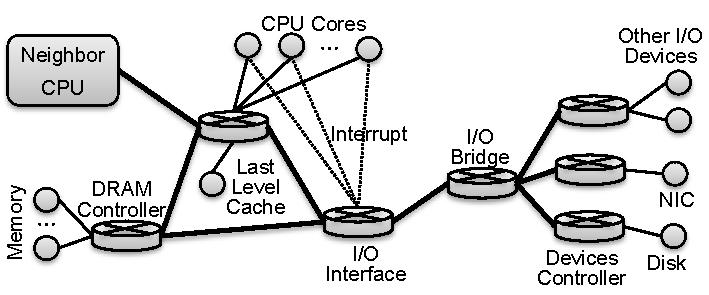
\includegraphics[height=4cm]{intro/computer-as-a-network.pdf}
  \caption[计算机内部本质是一个网络]{
    计算机内部部件之间以数据包(packet)进行通信,比如
    处理器核之间使用基于包的片上网络、
    处理器之间采用基于包的互连协议(如QPI和HT)、
    I/O设备与内存之间则通过PCI-E包进行通信。
    因此,计算机本身即可视为一个网络。}
  \label{fig:computer-as-a-network}
\end{figure}

基于以上需求,
本文提出了一种新体系结构:资源按需管理可编程的体系结构PARD\cite{pard:2015},
使数据中心服务器能够支持区分化服务,通过细粒度的硬件资源管理以及灵活的编程接口,
实现在保障关键应用服务质量的前提下提高服务器资源利用率。
PARD体系结构的核心是基于一个重要的观察:\textbf{计算机内部本质上是一个网络}。
如图\ref{fig:computer-as-a-network}所示,
CPU核、共享缓存、内存控制器、I/O设备等可以被看做是网络节点,它们之间通过包进行通信;
除了处理请求以外,这些``网络节点''与网络中的路由器/交换机具有相似的请求转发功能。
在网络领域,如何实现端到端的服务质量保障已有大量的研究,并已形成标准。
如IETF(Internet Engineering Task Force, 互联网工程任务组)于1998年提出了区分化服务
(Differentiated Services)\cite{DiffServ}的概念,
如今区分化服务已经成为应用最广泛的服务质量保障机制之一;
软件定义网络(SDN)\cite{SDN}的出现,进一步促进了网络领域服务质量保障的发展,其提出的
(1)控制平面与数据平面分离,和(2)集中控制的统一编程接口,
为网络管理带来了极大的灵活性。
本文希望能够将网络领域的区分化服务和软件定义网络的思想应用到计算机内部的网络,
用以解决数据中心当前面临的资源利用率与应用服务质量矛盾。

然而相比在计算机网络,
在体系结构这一``内部网络''中实现区分化服务与软件定义网络的功能需要面临一些额外的挑战:

首先,网络栈是整个网络中产生数据包的唯一位置,因此可以很容易的在其中增加标签机制,
实现网络流的区分。
而在计算机中有大量不同类型的硬件部件都能够向``内部网络''发送请求,
而且这些请求的类型各不相同,
如何为这些来自于不同硬件部件、类型各异的请求增加应用标签是需要解决的第一个挑战。

其次,与网络中交换机或路由器这些只进行存储转发的网络设备不同,
计算机内各个硬件部件通常包含更为复杂的功能,
如:处理器末级缓存需要为请求除完成将请求转发到下层内存控制器外,
还需要决定哪些请求数据缓存在本地,以及替换哪些数据到内存控制器;
内存控制器需要进行复杂的地址映射实现将物理地址映射到DRAM芯片,
同时还需要实现调度策略以提高访存性能;其他一些I/O设备具有更为复杂的功能。
因此如何为这些不同类型的硬件部分提供一个统一的控制平面实现对硬件资源的管理是第二个挑战。

最后,在交换机或路由器中已经为管理员提供了访问和配置其控制平面的固件接口,
而在当前的计算机中并没有类似的的固件接口。
服务器中普遍配置的IPMI/BMC\cite{ipmi}提供了诸如温度监控、电源控制、
BIOS访问等有限的监控与管理功能,利用该模块
如何实现硬件控制平面的管理,以及如何为用户(管理员)提供灵活的访问与编程接口是面临的第三个挑战。

为了解决以上三个挑战,PARD体系结构的核心设计理念可以归结为以下四点:
\textbf{1)标签机制},
通过在请求源(如处理器核或具有DMA功能的I/O设备)增加标签寄存器,使用其记录当前正在使用该部件的应用标签,
发出请求时附带该标签,并随着请求在整个计算机内部传播,实现应用区分;
\textbf{2)可编程控制平面},
为共享硬件资源的控制器增加控制平面,控制平面可根据请求标签查询规则进行区分处理,该规则可通过软件实现可编程;
\textbf{3)节点内统一资源管理},
节点内所有的控制平面通过控制平面网络连接到资源管理模块,提供对控制平面的编程接口,实现所有共享资源的统一管理;
\textbf{4)Trigger$\Rightarrow$Action编程方法},
一种基于动作触发的资源管理策略,实现资源实时监控和调整。

本文后续章节将讨论如何在现有体系结构上扩展以实现标签机制;
通用控制平面的设计以及可编程机制的实现,
并包括末级缓存控制器和内存控制器中控制平面的具体设计;
基于以上两种机制实现无Hypervisor的全硬件支持虚拟化系统,
以及如何实现资源按需分配的区分化服务,并使用模拟器对其效果进行验证。
最后在基于FPGA的原型系统中验证PARD体系结构的效果,
并讨论了原型系统实现过程中的经验与教训。


\section{本文的主要贡献}

本文的论点是:
在应用数量众多、需求多样且不断变化的数据中心场景下,计算机体系结构需要重新设计,
为应用提供区分化服务、良好的性能隔离,并具备灵活的资源管理编程接口,
实现资源使用的强控制与按需分配,
才能解决数据中心资源利用率与服务质量冲突的问题。

本文的主要贡献包括:

% 可在多个层次(虚拟机、进程、线程、API、...)区分应用,实现了NoHyper功能
第一,提出``标签化地址空间(Labeled Address Space)''概念。
正如多进程技术的出现引入了虚拟地址空间抽象,
随着虚拟化、云计算与多租户使用模式的出现,
现有的虚拟地址空间抽象无法满足多租户之间的隔离需求,
一些硬件隔离技术如EPT、I/O MMU、SR-IOV等试图在现有的体系结构下支持隔离需求,
其本质则是在虚拟地址空间外增加一层额外的地址空间,但这些技术只是在功能层面上实现了隔离,
而与性能相关的部件如共享末级缓存、内存控制器等在现有体系结构下并没有实现隔离。
本文提出的标签化地址空间抽象,使用统一标签区分不同应用,
并为计算机系统内所有请求标识应用标签,硬件不再需要通过猜测的方式区分应用,
而是通过标签机制打破目前体系结构中软硬件之间的语言鸿沟,
使得共享的硬件资源能够区分来自不同应用的请求并进行区分处理。
%可在不同层次实现应用区分,如虚拟机、进程、线程或使用API标识的数据/代码段,
%以实现不同粒度的区分化服务。
%以虚拟机粒度为例,通过标签机制以及共享硬件资源内部基于标签的划分机制,
%可将一台计算机划分为多台独立的逻辑域(Logical Domain),
%在每个逻辑域内独立运行操作系统,实现NoHyper\cite{keller_nohype:_2010}的功能。

% 表+Trigger/Action <=> 处理器方案
第二,提出硬件资源共享管理方法,为硬件资源共享提供配置、监控、反馈功能,
实现毫秒(ms)级的性能反馈。
%本文两个重要观点是:资源监控与管理结合,共享资源本地与全局协同管理结合。
实时的监控与反馈是实现细粒度资源管理的重要前提,软件监控方案无法满足实时性的需求,
在硬件上直接实现监控与反馈,提出使用通用的``控制平面''实现硬件资源的配置与监控。
在具体实现上,通过基于表的控制平面实现通用的硬件资源管理接口,
使用基于处理器的数据平面实现硬件请求的灵活控制,
为计算机系统实现硬件资源可管理提供支持。

第三,提出节点内硬件共享资源的协同管理。
控制平面构成了计算机系统内硬件资源管理的基本单元,由于硬件资源之间具有关联性,
需要进行全局统筹管理。
本文通过使用控制面网络将节点内所有的控制平面连接到集中式的资源管理模块,
对硬件共享资源进行协同管理。

以上三点贡献已在PARD的模拟器及FPGA原型系统中实现。
模拟器原型是基于gem5\cite{binkert_gem5_2011}实现的全系统时钟精确模拟器,
增加或修改了大约24,118行C++/Python代码,该模拟器以在LGPL协议下开源
\footnote{PARD-gem5模拟器开源地址https://github.com/fsg-ict/PARD-gem5}。
FPGA原型系统基于MicroBlaze系统在Xilinx VC709开发板实现并完成验证,
系统运行在133MHz频率,包含4个处理器核。
两个原型系统可以作为后续相关研究的参考平台。


\section{论文的组织}

\begin{figure}[htb]
  \centering
  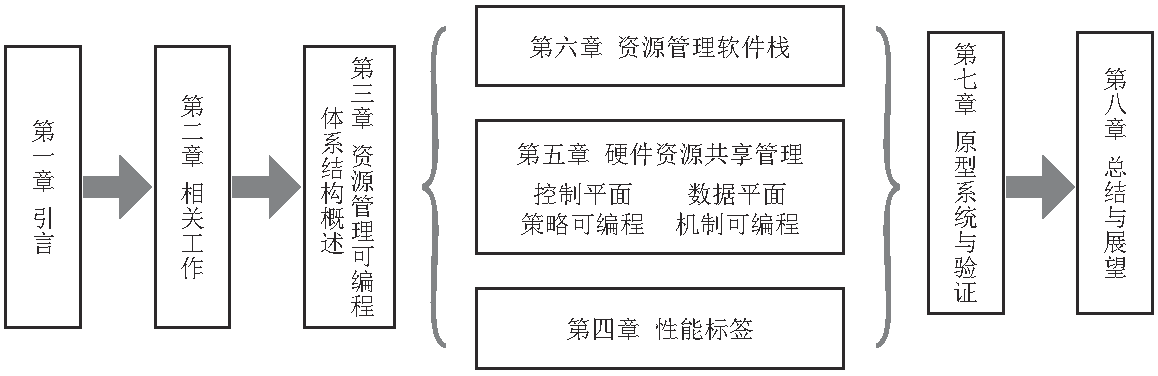
\includegraphics[width=\textwidth]{intro/thesis-structure}
  \caption{本文内容与组织结构}
  \label{fig:thesis-structure}
\end{figure}

本文共分八章,组织结构如图\ref{fig:thesis-structure}所示。

第二章介绍数据中心面临的资源利用率与服务质量冲突问题的挑战,
然后讨论现有数据中心技术的局限性,
并介绍解决该问题的现有研究。

第三章介绍PARD体系结构与关键特性,
并讨论如何利用PARD所提供的特性解决应用服务质量与资源利用率相冲突的问题。

第四章介绍PARD体系结构的基础标签化地址空间,
讨论在现有体系结构下实现标签化地址空间需要解决的关键问题,
并在模拟器上通过标签化地址空间改造,实现无软件支持的全硬件虚拟化功能。

第五章讨论硬件共享资源的管理方法,包括硬件资源的控制平面/数据平面抽象,
同时以共享末级缓存和内存控制器为例,讨论控制平面与数据平面的设计,
并通过模拟的方式验证该方案的有效性。

第六章介绍资源管理模块与资源协同管理相关的内容,包含节点内资源统一管理,
以及如何将PARD集成到现有的数据中心管理系统中(以Mesos\cite{Hindman:2011:Mesos}为例)。

第七章基于前四章的设计给出本文资源管理可编程体系结构的FPGA原型系统实现,
并对原型系统各部分功能的正确性、性能与开销进行评测。

第八章总结全文并介绍未来可能的研究工作。


% 
%%% Local Variables: 
%%% mode: latex
%%% TeX-master: t
%%% End: 

\chapter{相关研究}
\label{chap:related}

互联网应用如电子邮件、搜索、网络购物、社交网络、在线视频、网络地图等, 已经成为人们
生活的一部分。这些应用往往要为上亿用户服务,意味着互联网应用已变成如电力一样的社会
公共服务,而支撑拥有海量用户互联网应用的数据中心也成为如同发电厂一样的社会核心基础
设施。

长尾延迟(Tail Latency)问题在数据中心中受到越来越多的关注,造成长尾延迟的原因有很
多,其中最为重要的原因就是资源共享带来的干扰。
由于没有行之有效的方案对干扰进行控制,目前典型的数据中心都使用隔离的方式来减小干扰,
这一方案虽然有效缓解了长尾延迟,但它也带来了资源利用率过低的问题,
现有商用数据中心的资源利用率普遍只有10\%-30\%左右,造成极大的浪费。
如何解决服务质量与资源利用率的问题是当前业界面临的重大挑战。

本章内容安排如下:首先介绍新计算模式对数据中心的挑战,然后讨论现有数据中心技术的局
限性,即服务质量与资源利率冲突的原因,进而提出一种面向数据中心应用服务质量保障的
体系结构,最后将阐述本文的研究动机,介绍本文的主要贡献和组织结构。

%服务质量(QoS)与资源利用率是数据中心运营时需要考虑的两个重要指标,前者严重影响用户
%体验,而后者直接与数据中心的运营成本相关。然而现有的计算机体系结构并没有为服务质量
%保障提供足够的支持,造成这两个指标在现实状况下存在冲突。为了保障用户体验,在实际系
%统部署时,会更多的考虑服务质量这一指标,造成数据中心的资源利用率严重低下,普遍只有
%10\%-30\%左右。基于这一现状,本文主要讨论如何设计一种高效的数据中心体系结构,使得
%数据中心在保障应用服务质量基础上,达到较高的资源利用率。
%

\section{新计算模式对数据中心的挑战}

\subsection*{计算模式1:以云计算为基础的移动计算}

随着移动设备(平板电脑、智能手机)计算能力不断增强、成本不断降低以及无线通信技术的
快速发展,移动计算时代已经来临。如表\ref{tab:ganter-sales}所示,
Gartner调研数据显示平板电脑和手机(包含智能手机和普通手机)销量不断增加,
与此同时PC销量则不断下降。
而IDC预测到2015年智能手机销量将超过14亿部,占所有个人计算设备(包括PC、平板电脑和智能手机等)69\%的销量份额。

% Gartner关于电脑与移动设备销量的统计 
\begin{table}[htb]
  \centering
  \begin{minipage}[t]{0.9\linewidth}
  \caption[全球个人计算设备市场销量统计]{全球个人计算设备市场销量统计(单位:千部)}
  \label{tab:ganter-sales}
    \begin{tabular*}{\linewidth}{lrrrrr}
      \toprule[1.5pt]
      {\heiti 设备类型} & {\heiti 2012年} & {\heiti 2013年} & {\heiti 2014年} & {\heiti 2015年} & {\heiti 2016年} \\
      \midrule[1pt]
      PC(台式机、笔记本) &   341,273 &   296,131 &   279,000 &   259,000 &   248,000 \\ 
      超级本               &     9,787 &    21,517 &    39,000 &    62,000 &    85,000 \\ 
      平板电脑             &   120,203 &   206,807 &   216,000 &   233,000 &   259,000 \\ 
      手机                 & 1,746,177 & 1,806,964 & 1,838,000 & 1,906,000 & 1,969,000 \\ 
      其它移动设备         &       --- &     2,981 &     6,000 &     9,000 &    11,000 \\
      %总计                 & 2,217,440 & 2,334,400 & 2,378,000 & 2,470,000 & 2,572,000 \\
      \bottomrule[1.5pt]
    \end{tabular*}\\[2pt]
    \footnotesize
    数据来源:Gartner,2012年(http://www.gartner.com/newsroom/id/2610015),
    2013年(http://www.gartner.com-\\/newsroom/id/2791017),
    2014-2016年(http://www.gartner.com/newsroom/id/2954317)
  \end{minipage}
\end{table}

移动计算的快速发展带来新的计算模式:移动设备通过无线通信与运行在云计算平台的各类应
用服务进行交互。据可靠消息,目前一些主要的互联网公司(如Facebook和Baidu等)均表示,
来自移动设备的请求已占到40\%以上,并且仍在快速增长,很快将超过PC。随着4G时代的到来,
这种移动计算模式将成为未来的主流。

快速增长的移动计算需求对云计算平台的核心——数据中心带来了严峻的挑战。这种交互式计算
模式,快速的服务响应时间是衡量服务质量(Quality-of-Service,QoS)的关键指标,是让用
户满意、留住用户的关键。有研究表明,如果服务响应时间增加,公司收入就会减少。
例如,2009年微软在Bing搜索引擎上也开展实验,发现当服务响应时间增加到2000ms时,
每个用户带给企业的收益更是下降了4.3\%。由于该实验对公司产生了负面影响,最终不得不被
终止[8]。Amazon也发现其主页加载时间每增加100ms就会导致销售额下降1\% 。而Google更是
发现当搜索结果返回时间从0.4s增加到0.9s时,广告收入下降了20\%。

\begin{figure}
\begin{minipage}{0.48\textwidth}
  \centering
  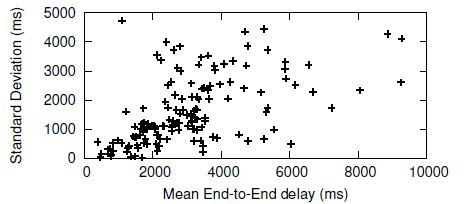
\includegraphics[height=5cm]{intro/end2end-delay}
  \caption[北美移动应用用户感知时延分布]{北美移动应用用户感知时延分布:平均延迟超过2秒且具有很大的波动性}
  \label{fig:end2end-delay}
\end{minipage}\hfill
\begin{minipage}{0.48\textwidth}
  \centering
  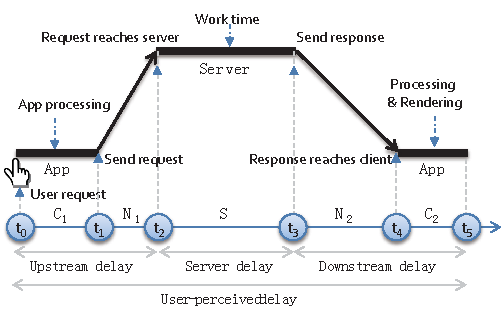
\includegraphics[height=5cm]{intro/interact-apps}
  \caption[一个典型的交互式请求的5个阶段]{一个典型的交互式请求的5个阶段:C1->N1->S->N2->C2 \cite{timecard2013}}
  \label{fig:interact-apps}
\end{minipage}
\end{figure}

移动计算的响应时间仍然存在很大的提升空间。
如图\ref{fig:end2end-delay}所示,微软公司实验数据表明在北美网络环境下,
交互式移动设备的平均时延超过2秒,而且存在较大的波动性。
图\ref{fig:interact-apps}显示典型移动交互式应用的用户请求时延分为5个阶段,
最近研究\cite{timecard2013}表明其中数据中心服务器的处理时延S约为1.2秒,占60\%。
随着4G网络的来临,数据中心将面临更大规模用户数据的处理请求。
因此,如何快速处理和及时响应移动计算请求将成为数据中心设计的核心目标之一。


\subsection*{计算模式2:面向大数据处理的实时计算}

大数据时代的到来使大数据处理架构受到越来越多的关注。2013年底中国计算机学会(CCF)
大数据专家委员会发布的《2014年大数据发展趋势十大预测》 报告中,来自学术界、产业界、
海外、跨界特邀和政府的122位专家们普遍认为,Hadoop/MapReduce框架一统天下的模式将被
打破,而实时流计算、分布式内存计算、图计算框架等将并存。

\begin{figure}[H]
  \centering
  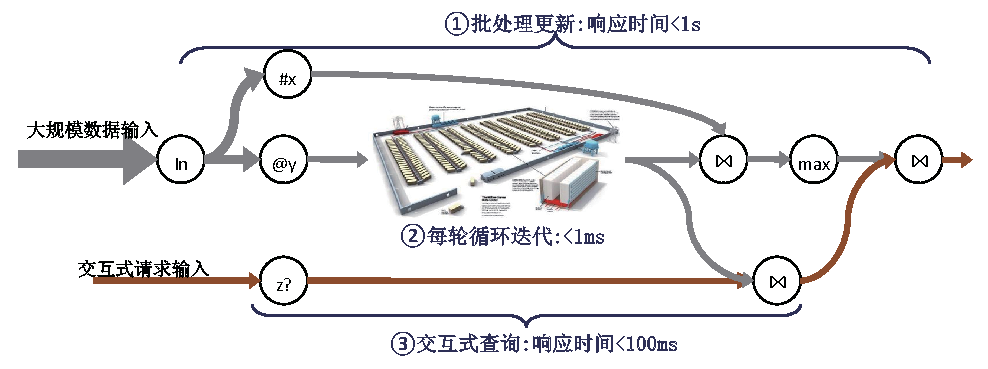
\includegraphics[height=6cm]{intro/batch-apps}
  \caption{典型的3类大数据处理需求以及相应的响应时间要求}
  \label{fig:batch-apps}
\end{figure}


大数据处理对数据中心和处理架构提出新的挑战,图\ref{fig:batch-apps}显示了典型的
大数据处理需求:首先需要支持数据的批处理更新模式(<1s);
其次数据处理会分解为多次迭代计算(<1ms);
再次还要支持实时计算模式,处理多用户的交互式查询请求(<100ms);
而这些处理所需要的数据
存放在同一个数据中心。搜索引擎是一个典型的例子,既需要对大规模网页进行内容处理,
迭代计算页面的pagerank,还需要处理大量用户的关键字查询请求。

尽管大数据处理希望能将各种处理集成在一个处理架构上,然后部署在一个数据中心。但如果
实时计算与企业营收相关,比如搜索引擎、在线购物等在线服务应用,那么正如微软Bing实验
所示,这些面向在线服务应用的实时计算的服务质量就非常关键(以下用“在线应用”
代表“实时计算”)。为了保障在线应用的服务质量,主流互联网企业一般将在线应用与大规模
批处理作业分别部署到不同的数据中心,以减少批处理作业对在线应用的干扰。但由于用户查
询请求数量具有显著的随时间变化的波动性,这种分离作业、单独部署的模式会导致在线应用
数据中心的资源平均利用率很低。如图4所示,Google的两类数据中心CPU利用率相差达2.5倍,
在线应用数据中心资源利用率仍有很大提升空间。


%% 典型的数据中心一般有5~10万台服务器组成,建设与运行维护成本往往高达几十亿人民
%% 币。然而出于保障应用服务质量的原因,现有数据中心只能维持较低的资源利用率,导致大量
%% 资源浪费。因此,本项目总体研究目标为如何设计高效通用数据中心体系结构:“通用”表
%% 示数据中心可同时运行各种不同类型应用;“高效”表示数据中心能在保障延迟敏感应用的服
%% 务质量基础上,达到较高的资源利用率(CPU利用率>60\%)。
%% 
%% 典型的数据中心一般有5~10万台中低端服务器组成,这些服务器通过内部网络互连,一起协同
%% 运行互联网应用为海量用户服务。因为这类数据中心规模很大,往往部署在大型仓库级别的机
%% 房,从应用角度来看就如同一台计算机,因此也被称为
%% “仓库级计算机(Warehouse-Scale Computer)“ \cite{WSC}。
%% 国内外著名的互联网公司往往拥有多个数据中心,服务器数量达到数十万甚
%% 至上百万台。例如,谷歌(Google)的数据中心服务器数量已经超过百万台为全球用户提供
%% 搜索、邮件、地图等服务[2];亚马逊(Amazon)仅EC2就部署了约50万台服务器提供云计算服
%% 务[3];据可靠消息,国内腾讯公司也拥有约30万服务器为用户提供各种互联网服务。
%% 
%% 尽管目前互联网企业的数据中心已经颇具规模,但一个趋势是未来数据中心还将持续发展。一
%% 方面互联网用户数量仍在不断增长,目前全球已有24亿网络用户,但很多机构预测未来全球还
%% 将新增30亿网民融入到互联网[4],这会对数据中心的数量和规模都提出更多需求。另一方面快
%% 速发展的移动终端已超越个人计算机(PC),成为终端计算设备的主流。由于移动设备性能相对
%% 较低、存储容量较小,将计算与存储转移到数据中心的需求也变得越来越强烈。因此数据中心作
%% 为基础设施也会日益重要。


\section{现有数据中心技术的局限性}

通过上述分析可知,移动计算与实时计算均对快速响应用户请求提出了强烈的需求。而当前数
据中心为了保障用户请求的服务质量,不得不通过采用牺牲资源利用率、保留过量资源的方式。
Google的数据中心技术一直处于领先地位,我们以Google为例分析数据中心资源利用率现状。
图\ref{fig:google-util-2006}显示了2006年Google数据中心平均CPU利用率为30\%左右。
但到2013年,虽然Google将数据中心分为了两类,并且批处理数据中心已经能达到75\%的CPU利用率,
但在线应用数据中心仍停留在30\%。
我们对国内企业调研发现,几大主流互联网企业在线应用数据中心CPU利用率一般都低于20\%,
有的甚至低于10\%,仍然存在很大的提升空间。

% Google数据中心利用率 
\begin{figure}
\begin{minipage}{0.57\textwidth}
  \centering
  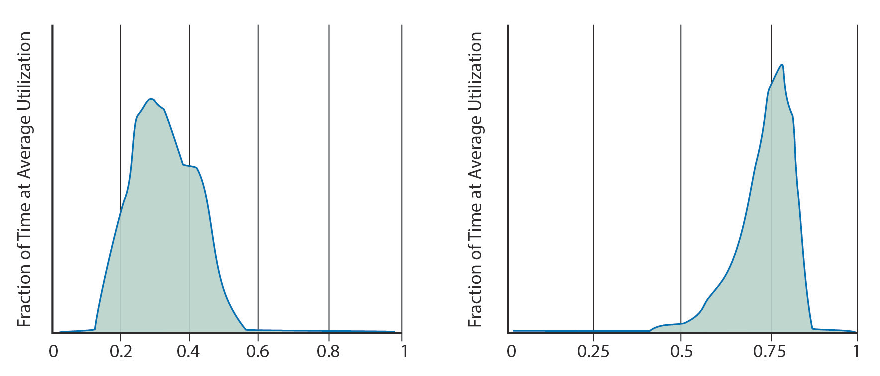
\includegraphics[height=4cm]{intro/google-util-2013}
  \caption[Google数据中心CPU利用率分布(2013年)]
    {Google数据显示2013年1至3月在线应用数据中心CPU利用率平均只有30\%(左图),
     而批处理作业数据中心则能达到75\%的利用率(两个数据中心均为2万台服务器)}
  \label{fig:google-util-2013}
\end{minipage}\hfill
\begin{minipage}{0.39\textwidth}
  \centering
  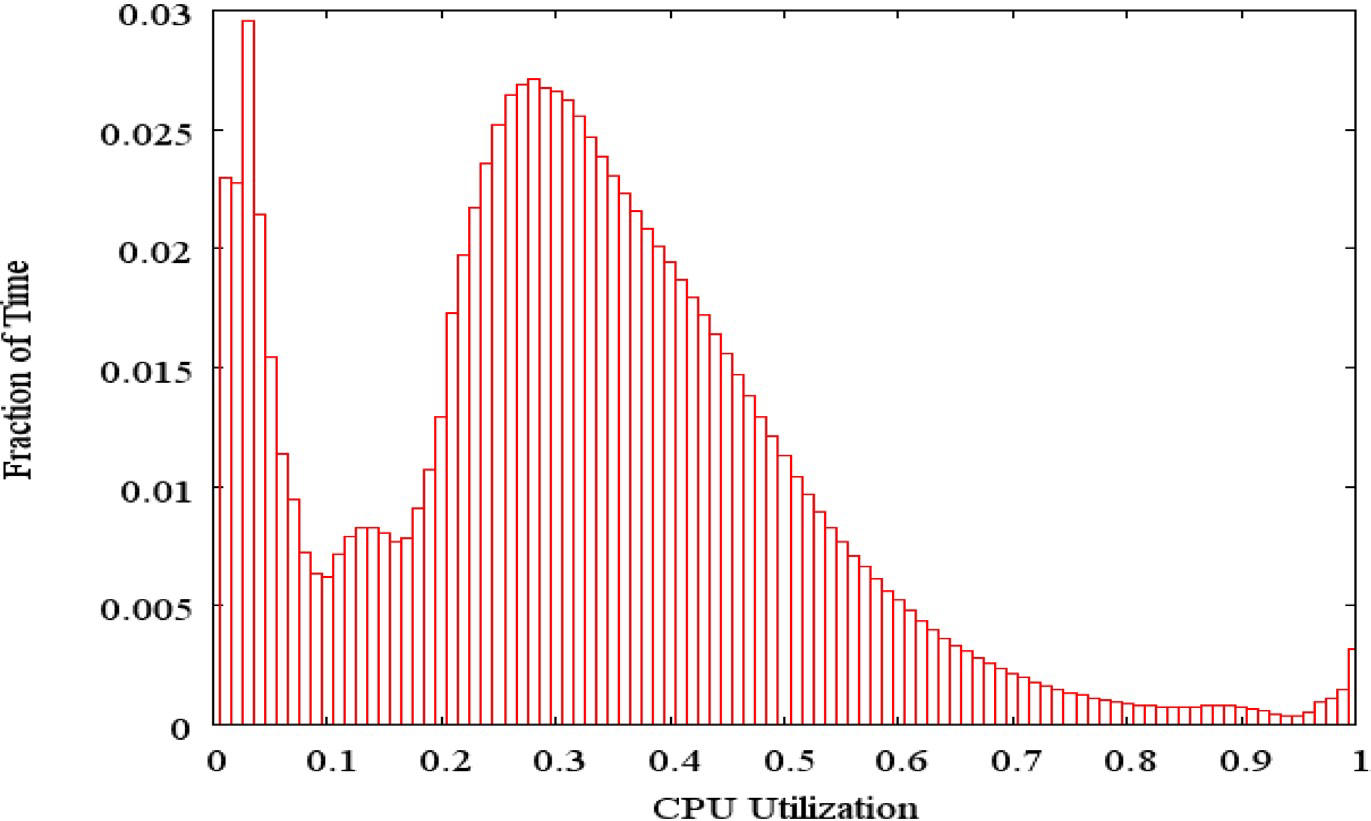
\includegraphics[height=3.5cm]{intro/google-util-2006}
  \caption[Google数据中心CPU利用率分布(2006年)]
    {Google在2006年数据中心(5000台服务器)6个月的CPU利用率分布}
  \label{fig:google-util-2006}
\end{minipage}
\end{figure}

尽管在线数据中心资源利用率只有30\%,但Google已经观察到严峻的长尾延迟现象---最慢的
1\%~10\%请求处理时间远大于所有请求的平均响应时间。
如图6所示,Google某后台服务延迟响应时间平均仅为5~6ms,但是却有相当一部分请求响应时间
超过了100ms[49]。而长尾延迟现象在数据中心环境下会被更进一步放大,因为一个用户请求需要
几百上千台服务器共同完成,只要有一台服务器的处理速度受到干扰,就会导致整个请求的处理
时间增加。Google的Jeff Dean在2012年Berkeley的报告[11]中就指出了长尾现象的严重性,假设
一台机器处理请求的平均响应时间为1ms,有1\%的请求为长尾处理时间会大于1s 
(99th-Percentile)。如果一个请求需要由100个这样的节点一起处理,那么就会出现63\%的请求
响应时间大于1s(如图7所示)。

造成在线应用数据中心资源利用率低和长尾延迟现象的核心原因是现有数据中心技术无法在多
应用混合运行时消除应用间干扰,以实现不同应用之间的性能隔离。
Google的Jeff Dean与Luiz Barroso在2013年2月的《Communication of the ACM》上撰文
“The Tail at Scale”[10]分析确认导致长尾延迟的首要原因就是资源共享,
包括体系结构层次的CPU核、Cache、访存带宽、网络带宽等,而干扰不仅来自应用,
还会来自系统软件层次的后台守护作业、监控作业、共享文件系统等。
Google在分布式架构和软件层次采用了多种缓解长尾延迟的技术,
包括操作系统容器隔离技术[12]、应用优先级管理[13]、备份请求[11]、同步后台管理进程[11]等,
取得了一定的效果,但却无法消除硬件体系结构层次上的应用之间的干扰,
导致仍然会出现图6这样的长尾延迟。

因此,现有数据中心处于“无管理的资源共享”状态,这
导致出现资源利用率与应用服务质量之间的矛盾:
一方面通过多个应用同时在数据中心部署实现资源共享能有效提高资源利用率,
但另一方面多个应用共享资源又会出现相互干扰严重影响应用的服务质量。
因此,目前企业不得不采用预留额外资源以保障延迟敏感的在线应用服务质量,
这导致很低的数据中心利用率。
而且随着多核技术的发展,单个服务器内的资源越来越多,
其上混合部署的应用数目也在不断增加,更会加剧这种矛盾。


\section{本文的研究动机}

现有数据中心技术面临资源利用率与应用服务质量的矛盾,其根本原因是大量数据中心共享资源
属于“无管理共享”状态。要实现高效通用数据中心目标,核心是从硬件上改变资源的“无
管理共享”现状以实现在体系结构上支持应用服务质量保障,在此基础上实现数据中心资源根据应
用动态管理以提高资源利用率。

回顾历史,当前数据中心面临的问题与1990年代的Internet具有相似之处。
当时流媒体、电子商务、电子邮件和FTP等大量网络应用的兴起,它们具有不同的QoS需求。
为了在IP网络中为这些应用提供端到端的服务质量保障,
互联网工程任务组(Internet Engineering Task Force, IETF)于1998年提出了区分化服务
(Differentiated Services)的概念。而如今,区分化服务已经成为应用最广泛的服务质量保障
机制之一。该技术的核心是在IP包头中定义长度为8-bit的区分化服务域,用以表示应用的
服务质量分类标识,因此路由器、交换机等网络设备便可以使用该信息对不同类别的数据包
进行区分处理,以达到区分化服务的目的。
软件定义网络(SDN)的出现,进一步促进了网络领域服务质量保障的发展,
其主要原理可以概括为:(1) 控制平面与数据平面分离;(2)集中控制的统一编程接口。

同时,计算机内部也可以被看做一个网络,如图\ref{fig:computer-as-a-network}所示,
CPU核、共享缓存、内存控制器、I/O设备等可以被看做是网络节点;除了处理请求以外,
这些“网络节点”与网络中的路由器/交换机具有相似的请求转发功能;
而它们之间也通过包进行通信,如:片内通信使用NoC包,片间通信的QPI/HT包,
以及I/O部分使用的PCI-E包。
将网络领域的区分化服务和软件定义网络的思想应用到计算机内部的网络,
用以解决数据中心当前面临的资源利用率与应用服务质量矛盾,是本文的主要研究思路与动机。

与在网络中部署SDN相比,在计算机体系结构“网络”中部署SDN会面临以下三个挑战:

首先,在整个网络栈中EndPoint是唯一的请求来源,因此SDN可以很容易的将标签机制实现在网络栈中;
与之相对的,在计算机体系结构中存在大量的硬件部件都能够发送请求,而这些请求类型又不尽相同,
因此在这样的环境下如何为请求打上标签是一个很大的挑战。

其次,在网络中所有的交换机都执行相同的存储/转发(store-and-forward)操作,但在计算机内部
不同的部件都有不同的功能,而不只是简单的存储/转发,如何为这些不同类型的部件(如末级缓存控制器、
内存控制器、I/O设备等)设计统一的控制面结构是另一个挑战。

最后,在网络交换机中已经包含了一个firmware固件用于访问和配置交换机的控制面,但计算机中却缺少
这样的firmware。现有的IPMI只被用来做有限的监控与管理功能,如对温度、风扇转速和电源控制。
因此,需要在计算机内部提供一种这样的部件实现与其它众多的控制面的通信与管理,并提供一个灵活的
编程接口对这些控制面进行操作。


%本项目总体研究目标是研究新型高效通用数据中心体系结构,能在保障应用服务质量
%的基础上将数据中心计算资源利用率提高到60\%以上。从技术挑战来看,计算机资源管理亟需新的
%具有以下特征的技术架构:
%(1)细粒度共享,有利于提高资源利用率;
%(2)性能隔离,有利于提高应用服务质量;
%(3)快速动态响应,有利于资源按需分配;
%(4)灵活协同配置,有利于协同多种资源配置以适应多种应用场景。


\section{论文的主要工作}

%本研究的目的是通过对真实环境、真实应用的访存行为特征进行更全面细致的分
%析,
%探索服务质量保障的体系结构支持,
%内存系统影响计算机整体性能的更深层次的原因,从而为体系结构、系统软件
%等的设计与优化提供一些建议。

%\begin{description}
% \item[First] \hfill \\
% The first item
% \item[Second] \hfill \\
% The second item
% \item[Third] \hfill \\
% The third etc \ldots
%\end{description}


本研究的目的是在体系结构层次解决数据中心所面临的资源利用率与服务质量相冲突的问题,
论文的主要工作围绕下述三个阶段开展:

\begin{itemize}
 \item 本研究在Xeon E5-v3平台上验证Cache容量划分功能对应用性能隔离带来的作用,
       并提出一种基于反馈模型的缓存自适应分配方法。
 \item 在体系结构内引入标签,实现应用区分,并在各个共享资源对其进行区分处理
 \item 提出一种资源管理可编程体系结构,实现可编程的硬件共享资源的细粒度管理
\end{itemize}


\section{论文的主要贡献}
In this paper, we propose Programmable Architecture for
Resourcing-on-Demand (PARD) that provides a new programming
interface to convey an application’s QoS requirements to the hardware.
PARD supports new functionalities such as fully hardwaresupported
virtualization without software hypervisors and differentiated
service (DiffServ) [60] in data center servers. For instance,
PARD can accurately isolate performance in shared data centers
to improve server utilization without degrading QoS for latencycritical
applications.



\section{论文的组织结构}

本文共分八章,第一章介绍移动计算带来的新计算模式对数据中心的挑战,然后讨论现有
数据中心技术的局限性,并针对现有体系结构提出了新的需求,最后介绍了论文的研究动机、
主要贡献和组织结构。

第二章介绍体系结构领域解决服务质量问题的现有研究,并对比以网络领域的相关内容,
讨论两者相互借鉴的可能性。

第三章对现有体系结构的服务质量支持进行评估,包括软件(cgroup, hyperviso)和硬件
两个层次。

第四章介绍资源管理可编程体系结构的概念与核心思路,并将其映射到现有体系结构,
讨论其可行性。同时应用资源管理可编程体系结构实现全硬件虚拟化,并讨论其关键技术。

第五章讨论模拟器实现,主要从功能设计角度对控制面设计,与资源管理可编程实现,
硬件支持、Trigger-Action机制,模拟的方式验证PARD的有效性。

第六章基于前两章的设计给出本文资源管理可编程体系结构的FPGA原型系统实现,
并对原型系统各部分功能的正确性、性能与开销进行了详细评测。

第七章在数据中心场景下,对本文资源管理可编程体系结构在分布式场景下应用进行讨论。

第八章总结全文并介绍未来可能的研究工作。


处理应用服务质量与资源利用率的问题,在互联网公司、芯片厂商还是学术界都在想办法解决
该问题:互联网公司方面,Baidu的Matrix项目、Google的Borg和Omega、Facebook的mesos系统
都尝试在软件架构层面解决该问题;Intel最新发布的Xeon E5-v3系列芯片,ARM芯片等都对QoS
提供了一定的支持;学术界在软硬件调度、划分方向也有大量工作。但这一问题并没有被解决,
本章首先介绍数据中心应用及其服务质量评价指标,并对现有工作进行总结,并分析其局限性。
同时参考网络领域在解决该问题的方案,

实现高效通用数据中心目标的前提在于保障应用服务质量。类似于系统安全需要所有环节安全
才能保障端到端(End-to-End)的安全,服务质量保障也需要应用全生命周期所有环节的支持。
在数据中心层面,这需要从服务器节点内部、服务器之间通信以及分布式架构多个层次协同工作。
近年来,学术界、工业界在这三个层次都不断努力。例如,近年来流行的Software Defined
Networking(SDN)技术\cite{SDN}目标就是解决数据中心网络通信的管理、共享与性能隔离问题。
Google在分布式架构上采用了超时发送备份请求同步后台管理进程等技术[11]来提高服务质量。
单节点内服务质量保障技术已成为短板。由于体系结构上不支持服务质量保障,而主流的软件
隔离技术能对资源容量隔离起到较好的效果,但无法保障性能隔离,无法保障服务质量。
总的来说,国内外在保障应用服务质量方面的研究包括单节点与分布式环境两个方面。
以下分别从这两个方面介绍相关工作。


应用混合的目标分为两方面:一是提高资源利用率,二是保障关键应用的服务质量。现有的运行时
管理方案[15]–[17]大都通过硬件性能计数器对关键应用的性能进行监控,并在性能发生下降时对非
关键应用进行各种处理,以减小由于资源竞争引起的性能问题。

造成资源利用率的核心问题在于计算机资源处于“无管理共享”状态,因此多个应用共享资源时会发
生竞争与干扰,最终导致关键应用性能不可预测。目前尚无很好的技术方案解决计算机资源“无管理
共享”的问题,以Google为代表的工业界采用将在线服务器与离线服务器分离的方法,通过降低在线
服务器的负载来保障在线应用的服务质量。

学术界在共享资源管理方面从2个维度、4个方面开展研究:软件调度、软件划分、硬件调度、硬件
划分。软件调度是通过操作系统/Hypervisor层次进行进程、线程或虚拟机级别的调度,一般调度粒
度较大,需要上下文切换,时间上也需要几毫秒到几十毫秒,不能满足在线应用的快时响应的需求;
软件划分技术能对Cache容量进行划分,但无法管理访存带宽这类资源,且软件划分技术配置调整开
销较大;硬件调度技术能支持访存请求级别的细粒度调度,但灵活性较多,不能根据不同应用按需管
理;硬件划分技术对Cache容量比较有效,但也无法对带宽等进行管理,而且同样面临灵活性差的问
题。面对诸多问题,斯坦福大学Christos Kozyrakis教授提出应该重新考虑整个计算机架构,从应用
特征、硬件隔离、操作系统、机群调度、高效资源管理硬件等多层次协同设计[18]。

\section{调度方法}
\label{sec:other}

实现高效通用数据中心目标的前提在于保障应用服务质量。类似于系统安全需要所有环节安全才能保障端到端(End-to-End)的安全,服务质量保障也需要应用全生命周期所有环节的支持。在数据中心层面,这需要从服务器节点内部、服务器之间通信以及分布式架构多个层次协同工作。近年来,学术界、工业界在这三个层次都不断努力。例如,近年来流行的Software Defined Networking(SDN)技术[15]目标就是解决数据中心网络通信的管理、共享与性能隔离问题。Google在分布式架构上采用了超时发送备份请求同步后台管理进程等技术[11]来提高服务质量。单节点内服务质量保障技术已成为短板。由于体系结构上不支持服务质量保障,而主流的软件隔离技术能对资源容量隔离起到较好的效果,但无法保障性能隔离,无法保障服务质量。

总的来说,国内外在保障应用服务质量方面的研究包括单节点与分布式环境两个方面。以下分别从这两个方面介绍相关工作。

1.2.1 单机保障服务质量研究

单机保障服务质量相关研究包括软件资源隔离技术、软硬件调度技术、硬件支持等。

软件隔离技术:针对数据中心里多个应用相互干扰的问题,一般采取虚拟化的手段在资源共享的条件下保障资源隔离,如虚拟机技术Xen[18]或Linux Container[17]。

传统虚拟机技术通过将多台虚拟机VM部署到物理机上,每台虚拟机运行一个应用或应用的一个组件,每个应用在自己的操作系统环境中独立运行,减少相互之间干扰。但这些隔离主要是资源的隔离,而无法实现性能隔离。例如为不同应用分配不同的访存带宽。而且使用虚拟机也会带来一定的性能损失[20],增加延迟,带来性能波动。

Linux Container[17]是一种轻量级虚拟化,通过在操作系统层面增添虚拟服务器功能,操作系统内核能够提供多个互相独立的用户态实例。每个用户态实例对于它自己的用户来说都像是一台独立的计算机,有自己独立的网络、文件系统、库函数和系统设置等。操作系统级虚拟化技术的优点是性能开销较小,不需要硬件的特别支持,而且能为用户态实例之间提供一定的隔离性,所以被广泛地应用在虚拟主机服务器环境中。然而,容器虚拟化技术的虚拟对象不是实际的物理资源(处理器、内存和外设),而是从用户角度出发而抽象的操作系统内部资源资,如CPU时间,内存,I/O带宽等,但如图1.5所示,Container技术对性能隔离效果并不理想。事实上,在性能隔离方面也有相关研究, Rice大学的Druschel等人[21]设计了Resource Container系统, 实现了单台物理机上多个应用间的性能隔离和CPU细粒度资源分配机制支持,然而局部隔离并不能保证全局隔离,Druschel 等人又设计了Cluster Container系统[22],以解决应用在集群范围内的隔离问题。但十几年前,单机核数目非常小,如今单节点已经有几十个核,同时运行的应用也增加了一个数量级,出现了很多新的挑战。

页着色(Page Coloring)[33]是一种以软件方式控制内存物理页映射到处理器缓存上的技术,映射到同一缓存块中的物理页对应同一颜色。基于页着色技术可以实现对共享二级缓存的划分(Partition)[36],能缓解应用在共享二级缓存上的干扰。Cho等人[34]使用Page Coloring技术来管理共享缓存。Tam等人[35]在Linux内核上实现了基于页面着色的缓存划分策略。而对于DRAM系统,也可以使用页着色技术对共享DRAM颗粒进行划分[37][39],例如,Liu等人[40]在Linux内核上实现了基于页着色的DRAM颗粒划分。北京大学李晓明教授团队也在这方面做了很多工作[41][42][43],研究利用页着色技术在虚拟环境下对共享Cache进行了划分。页着色技术能缓解一些粗粒度共享资源层次的干扰,但无法解决微体系结构的干扰,比如共享队列等,并且使用不灵活。总结而言,软件隔离技术能对资源容量隔离起到较好的效果,但无法保障性能隔离,无法保障服务质量。

软硬件调度:在多核微体系结构上,由于共享片上和片外资源的竞争会引起跨核应用之间的干扰。Jason Mars和Neil Vachharajani等人提出了竞争感知的轻量级运行时环境CAER[25],能在提高利用率的同时减少由竞争引起的跨核干扰问题。他还和Lingjia Tang等人在文章[24]还介绍了CiPE框架,可以直接用于测量和量化多核结构下应用的跨核干扰敏感度。Jason Mars等人还设计了Bubble-Up[23]机制,通过使用气泡(Bubble)来代表内存子系统的可变压力情况,能准确预测在内存子系统中竞争共享资源而导致的性能下降。Lingjia Tang等人在文章[29]提出了一种动静结合的编译方法ReQos,在确保高优先级应用的服务质量的同时让低优先级应用也可以自适应地执行。ReQoS包含一种由配置文件引导的编译技术,来识别低优先级应用中有争议的代码段。这些调度相关的工作,在具有大规模真实应用的Google“混布”数据中心里,使用该机制能在保证延迟敏感性应用的服务质量的同时,能显著提高50%~90%的资源利用率。但这些工作属于Ad-hoc类型,针对特定场景有效,并没有从根本上解决问题。

以CMU的Onur Mutlu为代表的一些学术界专家在提出了一系列调度算法[44][45][46]以缓解内存控制器的不公平问题,从而提高系统吞吐量以及服务质量。但这些算法是固化的,并不能针对某个应用进行调节,不具有灵活性。

体系结构支持:Ravi Iyer在文章[30]中提出了一种保障CMP体系结构上缓存Qos的管理框架,设计了CQos优先级分类、优先级分配和优先级执行。CQos优先级分类和优先级分配采用的是从用户到开发人员驱动的编译检测和基于流的方法;CQos优先级执行则包括(1)选择高速缓存分配、(2)动静态结合设置分区、(3)异构缓存区域。实验结果表明, CQoS在多线程或多核平台上能提高共享缓存的效率和系统性能。然而,文章[30]并没有详细描述保障CMP体系结构上缓存Qos的具体策略和软硬件支持。所以,Ravi Iyer等人又在文章[31]中实现了一种在CMP平台上保障Qos的内存体系结构,允运行时的动态资源再分配,能在减少低优先级应用性能下降的同时优化高优先级应用的性能。Andrew Herdrich等人[32]证明了用于功耗管理的基于速率(rate-based)的技术能适应于CMP结构上缓存/内存的Qos管理,其基本方法是当正在运行的低优先级任务由于资源争用而干扰了高优先级任务的性能时,就减缓核心的处理速率。通过评估时钟调制和频率缩放这两个速率限制机制,发现时钟调制更适用于缓存/内存Qos管理。

Ravi Iyer在体系结构支持服务质量方面做了一些有价值的工作,但主要集中在内存方面,并没有从整个系统角度去考虑。事实上,我们认为这个方向在未来会越来越重要,值得深入研究。
 
1.2.2 分布式环境保障服务质量

在分布式环境下,影响应用服务质量的因素主要是节点故障与干扰引起的长尾延迟,下面将从这两个方面介绍相关优化技术。

软硬件故障:Jean Dean等人设计MapReduce[26]的初衷是使用由成百上千机器组成的集群来处理超大规模的数据,所以,要求必须MapReduce能很好地处理机器故障。MapReduce采用了任务重新调度或重新执行任务(backup task)的方法来解决节点故障或短暂忙碌。比如,如果一个机器的硬盘出了问题,读取数据的速度从30M/s降低到1M/s, MapReduce框架中发送backup task机制来减少这一类长尾延迟。Backup task机制通常只会占用比正常操作多几个百分点的计算资源,但能显著改善因为故障出现的长尾延迟。不过,类似于TCP重传机制,backup task的有效性会随着负载的提高而削弱。


竞争共享资源引起的干扰:为了缓解干扰引起的长尾延迟现象,Dean等人[10]介绍了Google采用的缓解长尾延迟的技术,包括操作系统容器隔离技术[12]、应用优先级管理[13]、备份请求[11]、同步后台管理进程[11]等。R. Kapoor等人在文章[27]中提出了Chronos架构,以降低数据中心应用的长尾延迟。Chronos基于NIC上应用层数据包头字段的请求划分、应用实例负载均衡和NIC负载均衡模块的加载来消除关键通信路径上的共享资源,如内核和网络协议栈,以减少应用延迟以及相关干扰。

这些研究工作从分布式架构上一定程度上缓解了“划分/聚合”模式应用(如搜索、大数据分析等)的长尾延迟,但对“依赖/串行”模式(在线购物、社交等)应用并不显著。另一方面,随着单个服务器节点的核数目不断增加,甚至未来“片上数据中心”[47]出现,单节点内同时运行的应用也会增加,那么干扰将会越来越严重,仅仅依赖分布式架构以及软件方法将无法保障性能隔离,如何从硬件上支持服务质量保障技术将是一个值得关注与研究的方向。


\section{隔离方法}
\label{sec:multifig}

\section{软件定义网络SDN}
\label{sec:background:sdn}

The Need for a New Network Architecture % [REF] "Software-Defined Networking: The New Norm for Networks" (PDF). White paper. Open Networking Foundation. April 13, 2012. Retrieved August 22, 2013.
The explosion of mobile devices and content, server virtualization, and
advent of cloud services are among the trends driving the networking
industry to reexamine traditional network architectures. Many conventional
networks are hierarchical, built with tiers of Ethernet switches arranged in
a tree structure. This design made sense when client-server computing
was dominant, but such a static architecture is ill-suited to the dynamic
computing and storage needs of today’s enterprise data centers,
campuses, and carrier environments. Some of the key computing trends
driving the need for a new network paradigm include:


\section{本章小结}

从现有技术来看,单节点内服务质量保障技术的不足,导致节点内应用相互干扰严重,某种程
度上成为目前数据中心整体服务质量保障的短板,是成为长尾延迟现象的主要因素之一。同时
这也是一个非常具有挑战的问题,这需要跨层次协同设计。美国计算共同委员会(Computing 
Community Consortium)于2012年5月发布的计算机体系结构共同体白皮书《21世纪计算机体系
结构》中也将单节点内保障服务质量作为未来研究方向之一,其中认为[9]:“管理应用之间的相
互作用也带来了挑战。例如,这些应用如何表达服务质量(QoS)目标并且让底层的硬件、操作
系统以及虚拟层共同工作来保障它们。”


%
%
% %%% 其它部分
% \backmatter
% % 插图索引
% \listoffigures
% % 表格索引
% \listoftables
% % 公式索引
% \listofequations
%
%
% % 参考文献
% \bibliographystyle{ucasbib}
% \bibliography{ref/refs}
%
%
% % 致谢
% %%% Local Variables:
%%% mode: latex
%%% TeX-master: "../main"
%%% End:

\begin{ack}

转瞬在计算所读博的七年即将过去,这时才猛然发现,
和计算机相识已经16年了。
还记得初识时的CAI和LOGO,
还有那本似懂非懂的《数据结构:C语言描述》,
是我走上计算机道路的开始。
在这里要感谢那些给予我关怀、指导和帮助的人们。

首先要感谢我的导师孙凝晖老师,成为您的学生我的幸运。
您渊博的知识、严谨的治学态度和敏锐的思维,还有您对中国计算机事业的使命感,
是我今后学习的榜样。

还要感谢那些在重要的人生选择时给予我帮助的人:
感谢许强老师,是您将我从书本和实验带入到真正的项目,教会我需求分析、项目管理;
感谢董天正教授,是您带我进入到计算机系统结构领域;
感谢熊劲老师,您严谨的的治学态度,是我一直学习与坚持的榜样;
感谢李卓坚老师,是您手把手的教我认识机房与服务器,引领我进入系统管理的领域;
感谢马捷老师,您教会了我规范的重要。
特别要感谢包云岗老师,您是我的指路人,为我迷茫的博士路指明了方向,
也是在您的帮助下,我完成自己进入计算所时的梦想,造出了属于自己的计算机。

感谢计算所智能中心、高性能中心和先进计算机系统研究中心对我的培养。
感谢已经毕业的师兄们,
特别要感谢邢晶师兄、马灿师兄和李强师兄,是你们教会了我坚持与信念。
感谢与我共同奋斗的师弟师妹们:
感谢余子濠(濠神),我大PARD的重任就交给你了;
感谢黄博文、靳鑫,你们是我硬件入门的老师;
感谢展旭升、李宇鹏、徐天妮、姚治成、屈雨鹏、李文捷,和大家一起做科研是非常愉快的事情。
感谢张子刚,一起奋斗在博士的最后阶段,没有战友,一个人的战斗会非常的艰辛。

感谢徐志伟老师、冯晓兵老师、陈云霁老师、谢源老师、
孙广宇老师对我的学位论文提出了宝贵的修改意见。
感谢Donald E. Knuth以及Leslie Lamport,
他们开发的\TeX 和\LaTeX 使我可以专注于论文的写作。
还要感谢\ucasthesis 及其维护者xiaoyao9933,
它让我的论文写作轻松自在了许多,让我的论文格式规整漂亮了许多。

最后要感谢我的家人,感谢我的妈妈,
是您的关心与支持让我能够毫无顾虑的向着自己的理想奋斗,
您对我的爱是我一直前进的动力。

感谢我亲爱的妻子王一帆,一直默默的陪在我身边支持我、鼓励我,
是你的付出与理解,还有那些精心准备的爱心午餐,
让我能够专心科研、顺利毕业。

仅以此文,献给我的父亲。
\newline\newline

\rightline{2016年05月21日\qquad}
\rightline{于计算所\qquad\qquad}

\end{ack}

%
% % 附录
% \begin{appendix}
% %%% Local Variables: 
%%% mode: latex
%%% TeX-master: "../main"
%%% End: 

\chapter{外文资料原文}
\label{cha:engorg}
As one of the most widely used techniques in operations research, {\em
  mathematical programming} is defined as a means of maximizing a quantity known
as {\em objective function}, subject to a set of constraints represented by
equations and inequalities. Some known subtopics of mathematical programming are
linear programming, nonlinear programming, multiobjective programming, goal
programming, dynamic programming, and multilevel programming$^{[1]}$.

It is impossible to cover in a single chapter every concept of mathematical
programming. This chapter introduces only the basic concepts and techniques of
mathematical programming such that readers gain an understanding of them
throughout the book$^{[2,3]}$.


\section{Single-Objective Programming}
The general form of single-objective programming (SOP) is written
as follows,
\begin{equation}\tag*{(123)} % 如果附录中的公式不想让它出现在公式索引中,那就请
                             % 用 \tag*{xxxx}
\left\{\begin{array}{l}
\max \,\,f(x)\\[0.1 cm]
\mbox{subject to:} \\ [0.1 cm]
\qquad g_j(x)\le 0,\quad j=1,2,\cdots,p
\end{array}\right.
\end{equation}
which maximizes a real-valued function $f$ of
$x=(x_1,x_2,\cdots,x_n)$ subject to a set of constraints.

\newtheorem{mpdef}{Definition}[chapter]
\begin{mpdef}
In SOP, we call $x$ a decision vector, and
$x_1,x_2,\cdots,x_n$ decision variables. The function
$f$ is called the objective function. The set
\begin{equation}\tag*{(456)} % 这里同理,其它不再一一指定。
S=\left\{x\in\Re^n\bigm|g_j(x)\le 0,\,j=1,2,\cdots,p\right\}
\end{equation}
is called the feasible set. An element $x$ in $S$ is called a
feasible solution.
\end{mpdef}

\newtheorem{mpdefop}[mpdef]{Definition}
\begin{mpdefop}
A feasible solution $x^*$ is called the optimal
solution of SOP if and only if
\begin{equation}
f(x^*)\ge f(x)
\end{equation}
for any feasible solution $x$.
\end{mpdefop}

One of the outstanding contributions to mathematical programming was known as
the Kuhn-Tucker conditions\ref{eq:ktc}. In order to introduce them, let us give
some definitions. An inequality constraint $g_j(x)\le 0$ is said to be active at
a point $x^*$ if $g_j(x^*)=0$. A point $x^*$ satisfying $g_j(x^*)\le 0$ is said
to be regular if the gradient vectors $\nabla g_j(x)$ of all active constraints
are linearly independent.

Let $x^*$ be a regular point of the constraints of SOP and assume that all the
functions $f(x)$ and $g_j(x),j=1,2,\cdots,p$ are differentiable. If $x^*$ is a
local optimal solution, then there exist Lagrange multipliers
$\lambda_j,j=1,2,\cdots,p$ such that the following Kuhn-Tucker conditions hold,
\begin{equation}
\label{eq:ktc}
\left\{\begin{array}{l}
    \nabla f(x^*)-\sum\limits_{j=1}^p\lambda_j\nabla g_j(x^*)=0\\[0.3cm]
    \lambda_jg_j(x^*)=0,\quad j=1,2,\cdots,p\\[0.2cm]
    \lambda_j\ge 0,\quad j=1,2,\cdots,p.
\end{array}\right.
\end{equation}
If all the functions $f(x)$ and $g_j(x),j=1,2,\cdots,p$ are convex and
differentiable, and the point $x^*$ satisfies the Kuhn-Tucker conditions
(\ref{eq:ktc}), then it has been proved that the point $x^*$ is a global optimal
solution of SOP.

\subsection{Linear Programming} 
\label{sec:lp}

If the functions $f(x),g_j(x),j=1,2,\cdots,p$ are all linear, then SOP is called
a {\em linear programming}.

The feasible set of linear is always convex. A point $x$ is called an extreme
point of convex set $S$ if $x\in S$ and $x$ cannot be expressed as a convex
combination of two points in $S$. It has been shown that the optimal solution to
linear programming corresponds to an extreme point of its feasible set provided
that the feasible set $S$ is bounded. This fact is the basis of the {\em simplex
  algorithm} which was developed by Dantzig as a very efficient method for
solving linear programming.
\begin{table}[ht]
\centering
  \centering
  \caption*{Table~1\hskip1em This is an example for manually numbered table, which
    would not appear in the list of tables}
  \label{tab:badtabular2}
  \begin{tabular}[c]{|c|m{0.8in}|c|c|c|c|c|}\hline
    \multicolumn{2}{|c|}{Network Topology} & \# of nodes & 
    \multicolumn{3}{c|}{\# of clients} & Server \\\hline
    GT-ITM & Waxman Transit-Stub & 600 &
    \multirow{2}{2em}{2\%}& 
    \multirow{2}{2em}{10\%}& 
    \multirow{2}{2em}{50\%}& 
    \multirow{2}{1.2in}{Max. Connectivity}\\\cline{1-3}
    \multicolumn{2}{|c|}{Inet-2.1} & 6000 & & & &\\\hline
    \multirow{2}{1in}{Xue} & Rui  & Ni &\multicolumn{4}{c|}{\multirow{2}*{\ucasthesis}}\\\cline{2-3}
    & \multicolumn{2}{c|}{ABCDEF} &\multicolumn{4}{c|}{} \\\hline
\end{tabular}  
\end{table}

Roughly speaking, the simplex algorithm examines only the extreme points of the
feasible set, rather than all feasible points. At first, the simplex algorithm
selects an extreme point as the initial point. The successive extreme point is
selected so as to improve the objective function value. The procedure is
repeated until no improvement in objective function value can be made. The last
extreme point is the optimal solution.

\subsection{Nonlinear Programming}

If at least one of the functions $f(x),g_j(x),j=1,2,\cdots,p$ is nonlinear, then
SOP is called a {\em nonlinear programming}.

A large number of classical optimization methods have been developed to treat
special-structural nonlinear programming based on the mathematical theory
concerned with analyzing the structure of problems.
\begin{figure}[h]
  \centering
  
\includegraphics[clip]{thu-lib-logo}
  \caption*{Figure~1\hskip1em This is an example for manually numbered figure,
    which would not appear in the list of figures}
  \label{tab:badfigure2}    
\end{figure}

Now we consider a nonlinear programming which is confronted solely with
maximizing a real-valued function with domain $\Re^n$.  Whether derivatives are
available or not, the usual strategy is first to select a point in $\Re^n$ which
is thought to be the most likely place where the maximum exists. If there is no
information available on which to base such a selection, a point is chosen at
random. From this first point an attempt is made to construct a sequence of
points, each of which yields an improved objective function value over its
predecessor. The next point to be added to the sequence is chosen by analyzing
the behavior of the function at the previous points. This construction continues
until some termination criterion is met. Methods based upon this strategy are
called {\em ascent methods}, which can be classified as {\em direct methods},
{\em gradient methods}, and {\em Hessian methods} according to the information
about the behavior of objective function $f$. Direct methods require only that
the function can be evaluated at each point. Gradient methods require the
evaluation of first derivatives of $f$. Hessian methods require the evaluation
of second derivatives. In fact, there is no superior method for all
problems. The efficiency of a method is very much dependent upon the objective
function.

\subsection{Integer Programming}

{\em Integer programming} is a special mathematical programming in which all of
the variables are assumed to be only integer values. When there are not only
integer variables but also conventional continuous variables, we call it {\em
  mixed integer programming}. If all the variables are assumed either 0 or 1,
then the problem is termed a {\em zero-one programming}. Although integer
programming can be solved by an {\em exhaustive enumeration} theoretically, it
is impractical to solve realistically sized integer programming problems. The
most successful algorithm so far found to solve integer programming is called
the {\em branch-and-bound enumeration} developed by Balas (1965) and Dakin
(1965). The other technique to integer programming is the {\em cutting plane
  method} developed by Gomory (1959).

\hfill\textit{Uncertain Programming\/}\quad(\textsl{BaoDing Liu, 2006.2})

\section*{References}
\noindent{\itshape NOTE: these references are only for demonstration, they are
  not real citations in the original text.}

\begin{enumerate}[{$[$}1{$]$}]
\item Donald E. Knuth. The \TeX book. Addison-Wesley, 1984. ISBN: 0-201-13448-9
\item Paul W. Abrahams, Karl Berry and Kathryn A. Hargreaves. \TeX\ for the
  Impatient. Addison-Wesley, 1990. ISBN: 0-201-51375-7
\item David Salomon. The advanced \TeX book.  New York : Springer, 1995. ISBN:0-387-94556-3
\end{enumerate}

\chapter{外文资料的调研阅读报告或书面翻译}
\section{单目标规划}
北冥有鱼,其名为鲲。鲲之大,不知其几千里也。化而为鸟,其名为鹏。鹏之背,不知其几
千里也。怒而飞,其翼若垂天之云。是鸟也,海运则将徙于南冥。南冥者,天池也。 
\begin{equation}\tag*{(123)}
 p(y|\mathbf{x}) = \frac{p(\mathbf{x},y)}{p(\mathbf{x})}=
\frac{p(\mathbf{x}|y)p(y)}{p(\mathbf{x})}
\end{equation}

吾生也有涯,而知也无涯。以有涯随无涯,殆已!已而为知者,殆而已矣!为善无近名,为
恶无近刑,缘督以为经,可以保身,可以全生,可以养亲,可以尽年。

\subsection{线性规划}
庖丁为文惠君解牛,手之所触,肩之所倚,足之所履,膝之所倚,砉然响然,奏刀騞然,莫
不中音,合于桑林之舞,乃中经首之会。
\begin{table}[ht]
\centering
  \centering
  \caption*{表~1\hskip1em 这是手动编号但不出现在索引中的一个表格例子}
  \label{tab:badtabular3}
  \begin{tabular}[c]{|c|m{0.8in}|c|c|c|c|c|}\hline
    \multicolumn{2}{|c|}{Network Topology} & \# of nodes & 
    \multicolumn{3}{c|}{\# of clients} & Server \\\hline
    GT-ITM & Waxman Transit-Stub & 600 &
    \multirow{2}{2em}{2\%}& 
    \multirow{2}{2em}{10\%}& 
    \multirow{2}{2em}{50\%}& 
    \multirow{2}{1.2in}{Max. Connectivity}\\\cline{1-3}
    \multicolumn{2}{|c|}{Inet-2.1} & 6000 & & & &\\\hline
    \multirow{2}{1in}{Xue} & Rui  & Ni &\multicolumn{4}{c|}{\multirow{2}*{\ucasthesis}}\\\cline{2-3}
    & \multicolumn{2}{c|}{ABCDEF} &\multicolumn{4}{c|}{} \\\hline
\end{tabular}  
\end{table}

文惠君曰:“嘻,善哉!技盖至此乎?”庖丁释刀对曰:“臣之所好者道也,进乎技矣。始臣之
解牛之时,所见无非全牛者;三年之后,未尝见全牛也;方今之时,臣以神遇而不以目视,
官知止而神欲行。依乎天理,批大郤,导大窾,因其固然。技经肯綮之未尝,而况大坬乎!
良庖岁更刀,割也;族庖月更刀,折也;今臣之刀十九年矣,所解数千牛矣,而刀刃若新发
于硎。彼节者有间而刀刃者无厚,以无厚入有间,恢恢乎其于游刃必有余地矣。是以十九年
而刀刃若新发于硎。虽然,每至于族,吾见其难为,怵然为戒,视为止,行为迟,动刀甚微,
謋然已解,如土委地。提刀而立,为之而四顾,为之踌躇满志,善刀而藏之。”

文惠君曰:“善哉!吾闻庖丁之言,得养生焉。”


\subsection{非线性规划}
孔子与柳下季为友,柳下季之弟名曰盗跖。盗跖从卒九千人,横行天下,侵暴诸侯。穴室枢
户,驱人牛马,取人妇女。贪得忘亲,不顾父母兄弟,不祭先祖。所过之邑,大国守城,小
国入保,万民苦之。孔子谓柳下季曰:“夫为人父者,必能诏其子;为人兄者,必能教其弟。
若父不能诏其子,兄不能教其弟,则无贵父子兄弟之亲矣。今先生,世之才士也,弟为盗
跖,为天下害,而弗能教也,丘窃为先生羞之。丘请为先生往说之。”
\begin{figure}[h]
  \centering
  
\includegraphics{hello}
  \caption*{图~1\hskip1em 这是手动编号但不出现索引中的图片的例子}
  \label{tab:badfigure3}    
\end{figure}

柳下季曰:“先生言为人父者必能诏其子,为人兄者必能教其弟,若子不听父之诏,弟不受
兄之教,虽今先生之辩,将奈之何哉?且跖之为人也,心如涌泉,意如飘风,强足以距敌,
辩足以饰非。顺其心则喜,逆其心则怒,易辱人以言。先生必无往。”

孔子不听,颜回为驭,子贡为右,往见盗跖。

\subsection{整数规划}
盗跖乃方休卒徒大山之阳,脍人肝而餔之。孔子下车而前,见谒者曰:“鲁人孔丘,闻将军
高义,敬再拜谒者。”谒者入通。盗跖闻之大怒,目如明星,发上指冠,曰:“此夫鲁国之
巧伪人孔丘非邪?为我告之:尔作言造语,妄称文、武,冠枝木之冠,带死牛之胁,多辞缪
说,不耕而食,不织而衣,摇唇鼓舌,擅生是非,以迷天下之主,使天下学士不反其本,妄
作孝弟,而侥幸于封侯富贵者也。子之罪大极重,疾走归!不然,我将以子肝益昼餔之膳。”


\chapter{其它附录}
前面两个附录主要是给本科生做例子。其它附录的内容可以放到这里,当然如果你愿意,可
以把这部分也放到独立的文件中,然后将其 \verb|\input| 到主文件中。

% \end{appendix}
%
% % 个人简历
% \begin{resume}

\noindent
姓名:马久跃  性别:男  出生日期:1988.10.19  籍贯:辽宁\\

\noindent
2009.9 -- 现在       中国科学院计算技术所 计算机体系结构专业硕博研究生

\noindent
2005.9 -- 2009.7      东北师范大学软件学院 本科生\\

  \resumeitem{攻读博士学位期间发表的论文}
  \begin{enumerate}[leftmargin=1.5\parindent, nolistsep, label={[\arabic*]}]
    \item Jiuyue Ma, Xiufeng Sui, Ninghui Sun, Yupeng Li, Zihao Yu, Bowen Huang, Tianni Xu, Zhicheng Yao, Yu Chen, Haibin Wang, Lixin Zhang, Yungang Bao, Supporting Differentiated
    \item Jiuyue Ma, Xiufeng Sui, Yupeng Li, Zihao Yu, Bowen Huang, Yungang Bao, Supporting Differentiated Services in Datacenter Servers [C], OSDI'2014 Poster.
  \end{enumerate}

  \resumeitem{专利}
  \begin{enumerate}[leftmargin=1.5\parindent, nolistsep, label={[\arabic*]}]
    \item 马久跃,刘立坤,严得辰,李旭,基于设备能力的多终端数据同步方法和系统,申请号:201210208518.5,已授权
  \end{enumerate}

  \resumeitem{攻读博士学位期间参加的科研项目}
  \begin{enumerate}[leftmargin=1.5\parindent, nolistsep, label={[\arabic*]}]
    \item XX基金项目“共享存储机群系统的研究”(xxxxx),20xx年1月~20xx年12月
    \item 国家自然科学基金项目“共享存储机群系统中关键技术研究”(xxxxxxx),20xx年1月~20xx年12月
  \end{enumerate}

  \resumeitem{攻读博士学位期间的获奖情况}
  \begin{enumerate}[leftmargin=1.5\parindent, nolistsep, label={[\arabic*]}]
    \item 2011年被评为中国科学院``三好学生''
    \item 2012年获曙光博士奖学金
    \item 2015年获博士国家奖学金
  \end{enumerate}
\end{resume}

%
% \end{document}
% \end{example}
%
% \subsection{选项}
% \label{sec:option}
% 本模板提供了一些选项以方便使用:
% \begin{description}
% \item[master]
%   如果写硕士论文将此选项打开。
%   \begin{example}
% \documentclass[master]{ucasthesis}
%   \end{example}
%
% \item[doctor]
%   如果写博士论文将此选项打开。
%   \begin{example}
% \documentclass[doctor]{ucasthesis}
%   \end{example}
%
% \item[postdoctor]
%   如果写博士博士后出站报告将此选项打开。
%   \begin{example}
% \documentclass[postdoctor]{ucasthesis}
%   \end{example}
%
% \item[secret]
%   涉秘论文开关。配合另外两个命令 |\secretlevel| 和 |\secretyear| 分别用来指定保
%   密级别和时间。二者默认分别为\textbf{秘密}和当前年份。可以通过:
%   \cs{secretlevel}|{|绝密|}| 和 \cs{secretyear}|{|10|}| 年独立修改。
%   \begin{example}
% \documentclass[master, secret]{ucasthesis}
%   \end{example}
%
%
% \item[openany]
%   正规出版物的章节出现在奇数页,也就是右手边的页面,这就是 \texttt{openright},
%   也是 \ucasthesis 的默认选项。在这种情况下,如果前一章的最后一页也是奇数,那么
%   模板会自动生成一个纯粹的空白页,很多人不是很习惯这种方式,而且学校的格式似乎
%   更倾向于页面连续,那就是通常所说的 \texttt{openany}。{\fangsong 目前所有论文都是
%      openany。}这两个选项不用专门设置,\ucasthesis{} 会根据当前论文类型自动选
%   择。
%
%
% \item[arial]
%   使用真正的 arial 字体。此选项会装载 arial 字体宏包,如果此宏包不存在,就装
%   载Helvet。arialtoc 和 arialtitle 不受 arial 的影响。因为一般的 \TeX{} 发行都
%   没有 arial 字体,所以默认采用 Helvet,因为二者效果非常相似。如果你执着的要
%   用arial 字体,请参看:\href{http://www.mail-archive.com/ctan-ann@dante.de/msg00627.html}{Arial
%     字体}。
%
% \item[arialtoc]
%  目录项(章目录项除外)中的英文是否用 arial 字体。本选项和下一个 \textsl{arialtitle} 都不用用户
%  操心,模板都自动设置好了。
%
% \item[arialtitle]
%  章节标题中英文是否用 arial 字体(默认打开)。
% \end{description}
%
% \subsection{字体配置}
% \label{sec:font-config}
% 正确配置中文字体是使用模板的第一步。模板调用 ctex 宏包,提供如下字体使用方式:
% \begin{itemize}
%   \item 基于传统 CJK 包,使用 latex、pdflatex 编译;
%   \item 基于 xeCJK 包,使用 xelatex 编译。
% \end{itemize}
%
% 第一种方式的字体配置比较繁琐,建议使用 donated 制作的中文字体包(自
% 包含安装方法),请用户自行下载安装,此处不再赘述。本模板推荐使用第二
% 种方法,只要把所需字体放入系统字体文件夹(也可以指定自定义文件夹)即
% 可。
% 另外 Linux 系统缺少上述字体,这些用户可利用 fontname.def
% 文件配置所需字体。使用中易四种字体的配置如下:
% \begin{example}
% \ProvidesFile{fontname.def}
% \setCJKmainfont[BoldFont={SimHei},ItalicFont={KaiTi}]{SimSun}
% \setCJKsansfont{SimHei}
% \setCJKmonofont{FangSong}
% \setCJKfamilyfont{zhsong}{SimSun}
% \setCJKfamilyfont{zhhei}{SimHei}
% \setCJKfamilyfont{zhkai}{KaiTi}
% \setCJKfamilyfont{zhfs}{FangSong}
% \newcommand*{\songti}{\CJKfamily{zhsong}} % 宋体
% \newcommand*{\heiti}{\CJKfamily{zhhei}}   % 黑体
% \newcommand*{\kaishu}{\CJKfamily{zhkai}}  % 楷书
% \newcommand*{\fangsong}{\CJKfamily{zhfs}} % 仿宋
% \end{example}
%
% 对 Windows XP 来说如下,KaiTi 需要替换为 KaiTi\_GB2312,
% FangSong 需要替换为 FangSong\_GB2312。
%
% 宏包中包含了 ``zhfonts.py'' 脚本,为 Linux 用户提供一种交互式的方式
% 从系统中文字体中选择合适的六种字体,最终生成对应的 ``fontname.def''
% 文件。要使用它,只需在命令行输入该脚本的完整路径即可。
%
% 最后,用户可以通过命令
% \begin{shell}
% $ fs-list :lang=zh > zhfonts.txt
% \end{shell}
% 得到系统中现有的中文字体列表,并相应替换上述配置。
%
% \subsection{命令}
% \label{sec:command}
% 模板中的命令分为两类:一是格式控制,二是内容替换。格式控制如字体、字号、字距和
% 行距。内容替换如姓名、院系、专业、致谢等等。其中内容替换命令居多,而且主要集中
% 在封面上。首先来看格式控制命令。
%
% \subsubsection{基本控制命令}
% \label{sec:basiccom}
%
% \myentry{字体}
% \DescribeMacro{\songti}
% \DescribeMacro{\fangsong}
% \DescribeMacro{\heiti}
% \DescribeMacro{\kaishu}
% 等分别用来切换宋体、仿宋、黑体、楷体字体。
%
% \begin{example}
% {\songti 乾:元,亨,利贞}
% {\fangsong 初九,潜龙勿用}
% {\heiti 九二,见龙在田,利见大人}
% {\kaishu 九三,君子终日乾乾,夕惕若,厉,无咎}
% {\heiti 九五,飞龙在天,利见大人}
% {\songti 上九,亢龙有悔}
% \end{example}
%
% \myentry{字号}
% \DescribeMacro{\chuhao}
% 等命令定义一组字体大小,分别为:
%
% \begin{center}
% \begin{tabular}{lllll}
% \hline
% |\chuhao|&|\xiaochu|&|\yihao|&|\xiaoyi| &\\
% |\erhao|&|\xiaoer|&|\sanhao|&|\xiaosan|&\\
% |\sihao|& |\banxiaosi|&|\xiaosi|&|\dawu|&|\wuhao|\\
% |\xiaowu|&|\liuhao|&|\xiaoliu|&|\qihao|& |\bahao|\\\hline
% \end{tabular}
% \end{center}
%
% 使用方法为:\cs{command}\oarg{num},其中 |command| 为字号命令,|num| 为行距。比
% 如 |\xiaosi[1.5]| 表示选择小四字体,行距 1.5 倍。写作指南要求表格中的字体
% 是 \cs{dawu},模板已经设置好了。
%
% \begin{example}
% {\erhao 二号 \sanhao 三号 \sihao 四号  \qihao 七号}
% \end{example}
%
% \myentry{密级}
% \DescribeMacro{\secretlevel}
% \DescribeMacro{\secretyear}
% 定义秘密级别和年限:
%   \begin{example}
% \secretyear{5}
% \secretlevel{内部}
%   \end{example}
%
% \myentry{引用方式}
% \DescribeMacro{\onlinecite}

% 学校要求的参考文献引用有两种模式:(1)上标模式。比如``同样的工作有很
% 多$^{[1,2]}$\ldots''。(2)正文模式。比如``文[3] 中详细说明了\ldots''。其中上标
% 模式使用远比正文模式频繁,所以为了符合使用习惯,上标模式仍然用常规
% 的 |\cite{key}|,而 |\onlinecite{key}| 则用来生成正文模式。
%
% 关于参考文献模板推荐使用 \BibTeX{},关于中文参考文献需要额外增加一个 Entry: lang,将其设置为 \texttt{zh}
% 用来指示此参考文献为中文,以便 ucasbib.bst 处理。如:
% \begin{example}
% @INPROCEEDINGS{cnproceed,
%   author    = {王重阳 and 黄药师 and 欧阳峰 and 洪七公 and 段皇帝},
%   title     = {武林高手从入门到精通},
%   booktitle = {第~$N$~次华山论剑},
%   year      = 2006,
%   address   = {西安, 中国},
%   month     = sep,
%   lang      = "zh",
% }
%
% @ARTICLE{cnarticle,
%   AUTHOR  = "贾宝玉 and 林黛玉 and 薛宝钗 and 贾探春",
%   TITLE   = "论刘姥姥食量大如牛之现实意义",
%   JOURNAL = "红楼梦杂谈",
%   PAGES   = "260--266",
%   VOLUME  = "224",
%   YEAR    = "1800",
%   LANG    = "zh",
% }
% \end{example}
%
% \myentry{书脊}
% \DescribeMacro{\spine}
% 生成装订的书脊,为竖排格式,默认参数为论文中文题目。如果中文题目中没有英文字母,
% 那么直接调用此命令即可。否则,就要像例子里面那样做一些微调(参看模板自带
% 的 spine.tex)。下面是一个列子:
% \begin{example}
% \documentclass[master]{ucasthesis}
% \begin{document}
% \ctitle{论文中文题目}
% \cauthor{中文姓名}
% % |\spine| 命令需要上面两个变量
% \spine
%
% % 如果你的中文标题中有英文,那可以指定:
% \spine[中国科学院大学~\hspace{0.2em}\raisebox{2pt}{\LaTeX}%
% \hspace{-0.25em} 论文模板 \hspace{0.1em}\raisebox{2pt}%
% {v\version}\hspace{-0.25em}样例]
% \end{document}
% \end{example}
%
%
% \subsubsection{封面命令}
% \label{sec:titlepage}
% 下面是内容替换命令,其中以 |c| 开头的命令跟中文相关,|e| 开头则为对应的英文。
% 这部分的命令数目比较多,但实际上都相当简单,套用即可。
%
% 大多数命令的使用方法都是: \cs{command}\marg{arg},例外者将具体指出。这些命令都
% 在示例文档的 data/cover.tex 中。
%
% \myentry{论文标题}
% \DescribeMacro{\ctitle}
% \DescribeMacro{\etitle}
% \begin{example}
% \ctitle{论文中文题目}
% \etitle{Thesis English Title}
% \end{example}
%
% \myentry{作者姓名}
% \DescribeMacro{\cauthor}
% \DescribeMacro{\eauthor}
% \begin{example}
% \cauthor{中文姓名}
% \eauthor{Your name in PinYin}
% \end{example}
%
% \myentry{申请学位名称}
% \DescribeMacro{\cdegree}
% \DescribeMacro{\edegree}
% \begin{example}
% \cdegree{您要申请什么学位}
% \edegree{degree in English}
% \end{example}
%
% \myentry{院系名称}
% \DescribeMacro{\cdepartment}
% \DescribeMacro{\edepartment}
%
% \cs{cdepartment} 可以加一个可选参数,如:\cs{cdepartmentl}\oarg{精简}\marg{详
%   细},因为需要填写的空间有限,最好
% 给出一个详细和精简院系名称,如\textbf{计算机科学与技术}和\textbf{计算机}。
% \begin{example}
% \cdepartment[系名简称]{系名全称}
% \edepartment{Department}
% \end{example}
%
% \myentry{专业名称}
% \DescribeMacro{\cmajor}
% \DescribeMacro{\emajor}
% \begin{example}
% \cmajor{专业名称}
% \emajor{Major in English}
% \end{example}
%
% \DescribeMacro{\cfirstdiscipline}
% \DescribeMacro{\cseconddiscipline}
% \begin{example}
% \cfirstdiscipline{博士后一级学科}
% \cseconddiscipline{博士后二级学科}
% \end{example}
%
% \myentry{导师姓名}
% \DescribeMacro{\csupervisor}
% \DescribeMacro{\esupervisor}
% \begin{example}
% \csupervisor{导师~教授}
% \esupervisor{Supervisor}
% \end{example}
%
% \myentry{副导师姓名}
% \DescribeMacro{\cassosupervisor}
% \DescribeMacro{\eassosupervisor}
% \begin{example}
% \cassosupervisor{副导师~副教授}
% \eassosupervisor{Small Boss}
% \end{example}
%
% \myentry{联合导师}
% \DescribeMacro{\ccosupervisor}
% \DescribeMacro{\ecosupervisor}
% 硕士生联合指导教师,博士生联合导师。
% \begin{example}
% \ccosupervisor{联合导师~教授}
% \ecosupervisor{Tiny Boss}
% \end{example}
%
% \myentry{论文成文日期}
% \DescribeMacro{\cdate}
% \DescribeMacro{\edate}
% \DescribeMacro{\postdoctordate}
% 默认为当前时间,也可以自己指定。
% \begin{example}
% \cdate{中文日期}
% \edate{English Date}
% \postdoctordate{2009年7月——2011年7月} % 博士后研究起止日期
% \end{example}
%
% \myentry{博士后封面其它参数}
% \DescribeMacro{\catalognumber}
% \DescribeMacro{\udc}
% \DescribeMacro{\id}
% \begin{example}
% \catalognumber{分类号}
% \udc{udc}
% \id{编号}
% \end{example}
%
% \myentry{摘要}
% \DescribeEnv{cabstract}
% \DescribeEnv{eabstract}
% \begin{example}
% \begin{cabstract}
%  摘要请写在这里...
% \end{cabstract}
% \begin{eabstract}
%  here comes English abstract...
% \end{eabstract}
% \end{example}
%
% \myentry{关键词}
% \DescribeMacro{\ckeywords}
% \DescribeMacro{\ekeywords}
% 关键词用英文逗号分割写入相应的命令中,模板会解析各关键词并生成符合不同论文格式
% 要求的关键词格式。
% \begin{example}
% \ckeywords{关键词 1, 关键词 2}
% \ekeywords{keyword 1, key word 2}
% \end{example}
%
% \subsubsection{其它部分}
% \label{sec:otherparts}
% 论文其它主要部分命令:
%
% \myentry{符号对照表}
% \DescribeEnv{denotation}
% 主要符号表环境。简单定义的一个 list,跟 description 非常类似,使用方法参见示例
% 文件。带一个可选参数,用来指定符号列的宽度(默认为 2.5cm)。
% \begin{example}
% \begin{denotation}
%   \item[E] 能量
%   \item[m] 质量
%   \item[c] 光速
% \end{denotation}
% \end{example}
%
% 如果你觉得符号列的宽度不满意,那可以这样来调整:
% \begin{example}
% \begin{denotation}[1.5cm] % 设置为 1.5cm
%   \item[E] 能量
%   \item[m] 质量
%   \item[c] 光速
% \end{denotation}
% \end{example}
%
% \myentry{索引}
% 插图、表格和公式三个索引命令分别如下,将其插入到期望的位置即可(带星号的命令表
% 示对应的索引表不会出现在目录中):
%
% \begin{center}
% \begin{tabular}{ll}
% \hline
%   {\heiti 命令} & {\heiti 说明} \\\hline
% \cs{listoffigures} & 插图索引\\
% \cs{listoffigures*} & \\\hline
% \cs{listoftables} & 表格索引\\
% \cs{listoftables*} & \\\hline
% \cs{listofequations} & 公式索引\\
% \cs{listofequations*} & \\\hline
% \end{tabular}
% \end{center}
%
% \LaTeX{} 默认支持插图和表格索引,是通过 \cs{caption} 命令完成的,因此它们必须出
% 现在浮动环境中,否则不被计数。
%
% 有的同学不想让某个表格或者图片出现在索引里面,那么请使用命令 \cs{caption*},这
% 个命令不会给表格编号,也就是出来的只有标题文字而没有``表~xx'',``图~xx'',否则
% 索引里面序号不连续就显得不伦不类,这也是 \LaTeX{} 里星号命令默认的规则。
%
% 有这种需求的多是英文资料翻译部分,如果你觉得附录中英文原文中的表格和
% 图片显示成``表''和``图''很不协调的话,一个很好的办法还是用 \cs{caption*},参数
% 随便自己写,具体用法请参看示例文档。
%
% 如果你的确想让它编号,但又不想让它出现在索引中的话,那就自己改一改模板的代码吧,
% 我目前不打算给模板增加这种另类命令。
%
% 公式索引为本模板扩展,模板扩展了 \pkg{amsmath} 几个内部命令,使得公式编号样式和
% 自动索引功能非常方便。一般来说,你用到的所有数学环境编号都没问题了,这个可以参
% 看示例文档。如果你有个非常特殊的数学环境需要加入公式索引,那么请使
% 用 \cs{equcaption}\marg{编号}。此命令表示 equation caption,带一个参数,即显示
% 在索引中的编号。因为公式与图表不同,我们很少给一个公式附加一个标题,之所以起这
% 么个名字是因为图表就是通过 \cs{caption} 加入索引的,\cs{equcaption} 完全就是为
% 了生成公式列表,不产生什么标题。
%
% 使用方法如下。假如有一个非 equation 数学环境 mymath,只要在其中写一
% 句 \cs{equcaption} 就可以将它加入公式列表。
% \begin{example}
% \begin{mymath}
%   \label{eq:emc2}\equcaption{\ref{eq:emc2}}
%   E=mc^2
% \end{mymath}
% \end{example}
%
% 当然 mymath 正文中公式的编号需要你自己来做。
%
% 同图表一样,附录中的公式有时候也不希望它跟全文统一编号,而且不希望它出现在公式
% 索引中,目前的解决办法就是利用 \cs{tag*}\marg{公式编号} 来解决。用法很简单,此
% 处不再罗嗦,实例请参看示例文档附录 A 的前两个公式。
%
% \myentry{简历}
% \DescribeEnv{resume}\DescribeMacro{\resumeitem}
% 开启个人简历章节,包括发表文章列表等。其实就是一个 chapter。里面的每个子项目请用命令 |\resumeitem{sub title}|。
%
% 这里就不再列举例子了,请参看示例文档的 data/resume.tex。
%
% \myentry{附录}
% \DescribeEnv{appendix}
% 所有的附录都插到这里来。因为附录会更改默认的 chapter 属性,而后面的{\heiti 个人简
%   历}又需要恢复,所以实现为环境可以保证全局的属性不受影响。
% \begin{example}
% \begin{appendix}
%  %%% Local Variables: 
%%% mode: latex
%%% TeX-master: "../main"
%%% End: 

\chapter{外文资料原文}
\label{cha:engorg}
As one of the most widely used techniques in operations research, {\em
  mathematical programming} is defined as a means of maximizing a quantity known
as {\em objective function}, subject to a set of constraints represented by
equations and inequalities. Some known subtopics of mathematical programming are
linear programming, nonlinear programming, multiobjective programming, goal
programming, dynamic programming, and multilevel programming$^{[1]}$.

It is impossible to cover in a single chapter every concept of mathematical
programming. This chapter introduces only the basic concepts and techniques of
mathematical programming such that readers gain an understanding of them
throughout the book$^{[2,3]}$.


\section{Single-Objective Programming}
The general form of single-objective programming (SOP) is written
as follows,
\begin{equation}\tag*{(123)} % 如果附录中的公式不想让它出现在公式索引中,那就请
                             % 用 \tag*{xxxx}
\left\{\begin{array}{l}
\max \,\,f(x)\\[0.1 cm]
\mbox{subject to:} \\ [0.1 cm]
\qquad g_j(x)\le 0,\quad j=1,2,\cdots,p
\end{array}\right.
\end{equation}
which maximizes a real-valued function $f$ of
$x=(x_1,x_2,\cdots,x_n)$ subject to a set of constraints.

\newtheorem{mpdef}{Definition}[chapter]
\begin{mpdef}
In SOP, we call $x$ a decision vector, and
$x_1,x_2,\cdots,x_n$ decision variables. The function
$f$ is called the objective function. The set
\begin{equation}\tag*{(456)} % 这里同理,其它不再一一指定。
S=\left\{x\in\Re^n\bigm|g_j(x)\le 0,\,j=1,2,\cdots,p\right\}
\end{equation}
is called the feasible set. An element $x$ in $S$ is called a
feasible solution.
\end{mpdef}

\newtheorem{mpdefop}[mpdef]{Definition}
\begin{mpdefop}
A feasible solution $x^*$ is called the optimal
solution of SOP if and only if
\begin{equation}
f(x^*)\ge f(x)
\end{equation}
for any feasible solution $x$.
\end{mpdefop}

One of the outstanding contributions to mathematical programming was known as
the Kuhn-Tucker conditions\ref{eq:ktc}. In order to introduce them, let us give
some definitions. An inequality constraint $g_j(x)\le 0$ is said to be active at
a point $x^*$ if $g_j(x^*)=0$. A point $x^*$ satisfying $g_j(x^*)\le 0$ is said
to be regular if the gradient vectors $\nabla g_j(x)$ of all active constraints
are linearly independent.

Let $x^*$ be a regular point of the constraints of SOP and assume that all the
functions $f(x)$ and $g_j(x),j=1,2,\cdots,p$ are differentiable. If $x^*$ is a
local optimal solution, then there exist Lagrange multipliers
$\lambda_j,j=1,2,\cdots,p$ such that the following Kuhn-Tucker conditions hold,
\begin{equation}
\label{eq:ktc}
\left\{\begin{array}{l}
    \nabla f(x^*)-\sum\limits_{j=1}^p\lambda_j\nabla g_j(x^*)=0\\[0.3cm]
    \lambda_jg_j(x^*)=0,\quad j=1,2,\cdots,p\\[0.2cm]
    \lambda_j\ge 0,\quad j=1,2,\cdots,p.
\end{array}\right.
\end{equation}
If all the functions $f(x)$ and $g_j(x),j=1,2,\cdots,p$ are convex and
differentiable, and the point $x^*$ satisfies the Kuhn-Tucker conditions
(\ref{eq:ktc}), then it has been proved that the point $x^*$ is a global optimal
solution of SOP.

\subsection{Linear Programming} 
\label{sec:lp}

If the functions $f(x),g_j(x),j=1,2,\cdots,p$ are all linear, then SOP is called
a {\em linear programming}.

The feasible set of linear is always convex. A point $x$ is called an extreme
point of convex set $S$ if $x\in S$ and $x$ cannot be expressed as a convex
combination of two points in $S$. It has been shown that the optimal solution to
linear programming corresponds to an extreme point of its feasible set provided
that the feasible set $S$ is bounded. This fact is the basis of the {\em simplex
  algorithm} which was developed by Dantzig as a very efficient method for
solving linear programming.
\begin{table}[ht]
\centering
  \centering
  \caption*{Table~1\hskip1em This is an example for manually numbered table, which
    would not appear in the list of tables}
  \label{tab:badtabular2}
  \begin{tabular}[c]{|c|m{0.8in}|c|c|c|c|c|}\hline
    \multicolumn{2}{|c|}{Network Topology} & \# of nodes & 
    \multicolumn{3}{c|}{\# of clients} & Server \\\hline
    GT-ITM & Waxman Transit-Stub & 600 &
    \multirow{2}{2em}{2\%}& 
    \multirow{2}{2em}{10\%}& 
    \multirow{2}{2em}{50\%}& 
    \multirow{2}{1.2in}{Max. Connectivity}\\\cline{1-3}
    \multicolumn{2}{|c|}{Inet-2.1} & 6000 & & & &\\\hline
    \multirow{2}{1in}{Xue} & Rui  & Ni &\multicolumn{4}{c|}{\multirow{2}*{\ucasthesis}}\\\cline{2-3}
    & \multicolumn{2}{c|}{ABCDEF} &\multicolumn{4}{c|}{} \\\hline
\end{tabular}  
\end{table}

Roughly speaking, the simplex algorithm examines only the extreme points of the
feasible set, rather than all feasible points. At first, the simplex algorithm
selects an extreme point as the initial point. The successive extreme point is
selected so as to improve the objective function value. The procedure is
repeated until no improvement in objective function value can be made. The last
extreme point is the optimal solution.

\subsection{Nonlinear Programming}

If at least one of the functions $f(x),g_j(x),j=1,2,\cdots,p$ is nonlinear, then
SOP is called a {\em nonlinear programming}.

A large number of classical optimization methods have been developed to treat
special-structural nonlinear programming based on the mathematical theory
concerned with analyzing the structure of problems.
\begin{figure}[h]
  \centering
  
\includegraphics[clip]{thu-lib-logo}
  \caption*{Figure~1\hskip1em This is an example for manually numbered figure,
    which would not appear in the list of figures}
  \label{tab:badfigure2}    
\end{figure}

Now we consider a nonlinear programming which is confronted solely with
maximizing a real-valued function with domain $\Re^n$.  Whether derivatives are
available or not, the usual strategy is first to select a point in $\Re^n$ which
is thought to be the most likely place where the maximum exists. If there is no
information available on which to base such a selection, a point is chosen at
random. From this first point an attempt is made to construct a sequence of
points, each of which yields an improved objective function value over its
predecessor. The next point to be added to the sequence is chosen by analyzing
the behavior of the function at the previous points. This construction continues
until some termination criterion is met. Methods based upon this strategy are
called {\em ascent methods}, which can be classified as {\em direct methods},
{\em gradient methods}, and {\em Hessian methods} according to the information
about the behavior of objective function $f$. Direct methods require only that
the function can be evaluated at each point. Gradient methods require the
evaluation of first derivatives of $f$. Hessian methods require the evaluation
of second derivatives. In fact, there is no superior method for all
problems. The efficiency of a method is very much dependent upon the objective
function.

\subsection{Integer Programming}

{\em Integer programming} is a special mathematical programming in which all of
the variables are assumed to be only integer values. When there are not only
integer variables but also conventional continuous variables, we call it {\em
  mixed integer programming}. If all the variables are assumed either 0 or 1,
then the problem is termed a {\em zero-one programming}. Although integer
programming can be solved by an {\em exhaustive enumeration} theoretically, it
is impractical to solve realistically sized integer programming problems. The
most successful algorithm so far found to solve integer programming is called
the {\em branch-and-bound enumeration} developed by Balas (1965) and Dakin
(1965). The other technique to integer programming is the {\em cutting plane
  method} developed by Gomory (1959).

\hfill\textit{Uncertain Programming\/}\quad(\textsl{BaoDing Liu, 2006.2})

\section*{References}
\noindent{\itshape NOTE: these references are only for demonstration, they are
  not real citations in the original text.}

\begin{enumerate}[{$[$}1{$]$}]
\item Donald E. Knuth. The \TeX book. Addison-Wesley, 1984. ISBN: 0-201-13448-9
\item Paul W. Abrahams, Karl Berry and Kathryn A. Hargreaves. \TeX\ for the
  Impatient. Addison-Wesley, 1990. ISBN: 0-201-51375-7
\item David Salomon. The advanced \TeX book.  New York : Springer, 1995. ISBN:0-387-94556-3
\end{enumerate}

\chapter{外文资料的调研阅读报告或书面翻译}
\section{单目标规划}
北冥有鱼,其名为鲲。鲲之大,不知其几千里也。化而为鸟,其名为鹏。鹏之背,不知其几
千里也。怒而飞,其翼若垂天之云。是鸟也,海运则将徙于南冥。南冥者,天池也。 
\begin{equation}\tag*{(123)}
 p(y|\mathbf{x}) = \frac{p(\mathbf{x},y)}{p(\mathbf{x})}=
\frac{p(\mathbf{x}|y)p(y)}{p(\mathbf{x})}
\end{equation}

吾生也有涯,而知也无涯。以有涯随无涯,殆已!已而为知者,殆而已矣!为善无近名,为
恶无近刑,缘督以为经,可以保身,可以全生,可以养亲,可以尽年。

\subsection{线性规划}
庖丁为文惠君解牛,手之所触,肩之所倚,足之所履,膝之所倚,砉然响然,奏刀騞然,莫
不中音,合于桑林之舞,乃中经首之会。
\begin{table}[ht]
\centering
  \centering
  \caption*{表~1\hskip1em 这是手动编号但不出现在索引中的一个表格例子}
  \label{tab:badtabular3}
  \begin{tabular}[c]{|c|m{0.8in}|c|c|c|c|c|}\hline
    \multicolumn{2}{|c|}{Network Topology} & \# of nodes & 
    \multicolumn{3}{c|}{\# of clients} & Server \\\hline
    GT-ITM & Waxman Transit-Stub & 600 &
    \multirow{2}{2em}{2\%}& 
    \multirow{2}{2em}{10\%}& 
    \multirow{2}{2em}{50\%}& 
    \multirow{2}{1.2in}{Max. Connectivity}\\\cline{1-3}
    \multicolumn{2}{|c|}{Inet-2.1} & 6000 & & & &\\\hline
    \multirow{2}{1in}{Xue} & Rui  & Ni &\multicolumn{4}{c|}{\multirow{2}*{\ucasthesis}}\\\cline{2-3}
    & \multicolumn{2}{c|}{ABCDEF} &\multicolumn{4}{c|}{} \\\hline
\end{tabular}  
\end{table}

文惠君曰:“嘻,善哉!技盖至此乎?”庖丁释刀对曰:“臣之所好者道也,进乎技矣。始臣之
解牛之时,所见无非全牛者;三年之后,未尝见全牛也;方今之时,臣以神遇而不以目视,
官知止而神欲行。依乎天理,批大郤,导大窾,因其固然。技经肯綮之未尝,而况大坬乎!
良庖岁更刀,割也;族庖月更刀,折也;今臣之刀十九年矣,所解数千牛矣,而刀刃若新发
于硎。彼节者有间而刀刃者无厚,以无厚入有间,恢恢乎其于游刃必有余地矣。是以十九年
而刀刃若新发于硎。虽然,每至于族,吾见其难为,怵然为戒,视为止,行为迟,动刀甚微,
謋然已解,如土委地。提刀而立,为之而四顾,为之踌躇满志,善刀而藏之。”

文惠君曰:“善哉!吾闻庖丁之言,得养生焉。”


\subsection{非线性规划}
孔子与柳下季为友,柳下季之弟名曰盗跖。盗跖从卒九千人,横行天下,侵暴诸侯。穴室枢
户,驱人牛马,取人妇女。贪得忘亲,不顾父母兄弟,不祭先祖。所过之邑,大国守城,小
国入保,万民苦之。孔子谓柳下季曰:“夫为人父者,必能诏其子;为人兄者,必能教其弟。
若父不能诏其子,兄不能教其弟,则无贵父子兄弟之亲矣。今先生,世之才士也,弟为盗
跖,为天下害,而弗能教也,丘窃为先生羞之。丘请为先生往说之。”
\begin{figure}[h]
  \centering
  
\includegraphics{hello}
  \caption*{图~1\hskip1em 这是手动编号但不出现索引中的图片的例子}
  \label{tab:badfigure3}    
\end{figure}

柳下季曰:“先生言为人父者必能诏其子,为人兄者必能教其弟,若子不听父之诏,弟不受
兄之教,虽今先生之辩,将奈之何哉?且跖之为人也,心如涌泉,意如飘风,强足以距敌,
辩足以饰非。顺其心则喜,逆其心则怒,易辱人以言。先生必无往。”

孔子不听,颜回为驭,子贡为右,往见盗跖。

\subsection{整数规划}
盗跖乃方休卒徒大山之阳,脍人肝而餔之。孔子下车而前,见谒者曰:“鲁人孔丘,闻将军
高义,敬再拜谒者。”谒者入通。盗跖闻之大怒,目如明星,发上指冠,曰:“此夫鲁国之
巧伪人孔丘非邪?为我告之:尔作言造语,妄称文、武,冠枝木之冠,带死牛之胁,多辞缪
说,不耕而食,不织而衣,摇唇鼓舌,擅生是非,以迷天下之主,使天下学士不反其本,妄
作孝弟,而侥幸于封侯富贵者也。子之罪大极重,疾走归!不然,我将以子肝益昼餔之膳。”


\chapter{其它附录}
前面两个附录主要是给本科生做例子。其它附录的内容可以放到这里,当然如果你愿意,可
以把这部分也放到独立的文件中,然后将其 \verb|\input| 到主文件中。

%  \input{data/appendix02}
% \end{appendix}
% \end{example}
%
% \myentry{致谢声明}
% \DescribeEnv{ack}
% 把致谢做成一个环境更好一些,直接往里面写感谢的话就可以啦!下面是数学系一位同
% 学致谢里的话,拿过来做个广告,多希望每个人都能写这么一句啊!
% \begin{example}
% \begin{ack}
%   ……
%   还要特别感谢清华大学计算机系薛瑞尼同学在论文格式等方面给我的很多帮助!
%   顺便感谢下中科院计算所朝鲁同学对论文格式的修改!
% \end{ack}
% \end{example}
%
% \myentry{列表环境}
% \DescribeEnv{itemize}
% \DescribeEnv{enumerate}
% \DescribeEnv{description}
% 为了适合中文习惯,模板将这三个常用的列表环境用 \pkg{paralist} 对应的压缩环境替
% 换。一方面满足了多余空间的清楚,另一方面可以自己指定标签的样式和符号。细节请参
% 看 \pkg{paralist} 文档,此处不再赘述。
%
%
% \subsection{数学环境}
% \label{sec:math}
% \ucasthesis{} 定义了常用的数学环境:
%
% \begin{center}
% \begin{tabular}{*{7}{l}}\hline
%   axiom & theorem & definition & proposition & lemma & conjecture &\\
%   公理 & 定理 & 定义 & 命题 & 引理 & 猜想 &\\\hline
%   proof & corollary & example & exercise & assumption & remark & problem \\
%   证明 & 推论 & 例子& 练习 & 假设 & 注释 & 问题\\\hline
% \end{tabular}
% \end{center}
%
% 比如:
% \begin{example}
% \begin{definition}
% 道千乘之国,敬事而信,节用而爱人,使民以时。
% \end{definition}
% \end{example}
% 产生(自动编号):\\[5pt]
% \fbox{{\heiti 定义~1.1~~~} {道千乘之国,敬事而信,节用而爱人,使民以时。}}
%
% 列举出来的数学环境毕竟是有限的,如果想用{\heiti 胡说}这样的数学环境,那么很容易定义:
% \begin{example}
% \newtheorem{nonsense}{胡说}[chapter]
% \end{example}
%
% 然后这样使用:
% \begin{example}
% \begin{nonsense}
% 契丹武士要来中原夺武林秘笈。—— 慕容博
% \end{nonsense}
% \end{example}
% 产生(自动编号):\\[5pt]
% \fbox{{\heiti 胡说~1.1~~~} {契丹武士要来中原夺武林秘笈。\kern0.3ex\rule[0.8ex]{2em}{0.1ex}\kern0.3ex 慕容博}}
%
% \subsection{自定义以及其它}
% \label{sec:othercmd}
% 模板的配置文件 ucasthesis.cfg 中定义了很多固定词汇,一般无须修改。如果有特殊需求,
% 推荐在导言区使用 \cs{renewcommand}。当然,导言区里可以直接使用中文。
%
%
% \section{ThuThesis致谢}
% \label{sec:thanks}
% 感谢这些年来一直陪伴 ThuThesis 成长的新老同学,大家的需求是模板前
% 进的动力,大家的反馈是模板提高的机会。
% 
% 此版本加入了博士后出站报告的支持,本意为制作一个支持清华所有学位报告
% 的模板,孰料学校于近期对硕士、博士论文规范又有调整,未能及时更新,见
% 谅!
%
% 本人已于近期离开清华,虽不忍模板存此瑕疵,然精力有限,必不能如往日及
% 时升级,还望新的同学能参与或者接手,继续为大家服务。
% 
% \section{UCASThesis致谢}
% 感谢ThuThesis模板的作者,为国内学位论文模板提供了良好的实现基础。
%
% 感谢吴凯编写的GBT7714-2005N.bst,方便的解决了本模板文献格式问题。
% 
% 同时基于 ThuThesis 修改的版本 UCASThesis 离不开首批试用该模板的林健博士,
% 唐帝鑫, 杨阳师兄提出的宝贵修改意见。在此,我要特别感谢林健博士为此模板
% 精心的校对、修正所付出的辛勤汗水。没有林健博士对我的督促、帮助,
% 不会有该模板的诞生。
% 希望国科大的同学们继续完善该模板,欢迎fork, 但我更希望各分支版本能够
% 发起pull request造福更多同学。
%
% \StopEventually{\PrintChanges\PrintIndex}
% \clearpage
%
% \section{实现细节}
%
% \subsection{基本信息}
%    \begin{macrocode}
%<cls>\NeedsTeXFormat{LaTeX2e}[1999/12/01]
%<cls>\ProvidesClass{ucasthesis}
%<cfg>\ProvidesFile{ucasthesis.cfg}
%<cls|cfg>[2012/07/28 4.8dev University of Chinese Academy of Sciences Thesis Template]
%    \end{macrocode}
%
% \subsection{定义选项}
% \label{sec:defoption}
% TODO: 所有的选项用 \pkg{xkeyval} 来重构,现在的太罗唆了。
%
% 定义论文类型以及是否涉密
%    \begin{macrocode}
%<*cls>
\hyphenation{ucas-Thesis}
\def\ucasthesis{\textsc{ucasthesis}}
\def\version{4.8dev}
\newif\ifucas@master\ucas@masterfalse
\newif\ifucas@doctor\ucas@doctorfalse
\newif\ifucas@secret\ucas@secretfalse
\DeclareOption{master}{\ucas@mastertrue}
\DeclareOption{doctor}{\ucas@doctortrue}
\DeclareOption{secret}{\ucas@secrettrue}
%    \end{macrocode}
%
%
% 如果需要使用 arial 字体,请打开 [arial] 选项
%    \begin{macrocode}
\newif\ifucas@arial   %!
\DeclareOption{arial}{\ucas@arialtrue}
%    \end{macrocode}
%
% 目录中英文是否用 arial
%    \begin{macrocode}
\newif\ifucas@arialtoc
\DeclareOption{arialtoc}{\ucas@arialtoctrue}
%    \end{macrocode}
% 章节标题中的英文是否用 arial
%    \begin{macrocode}
\newif\ifucas@arialtitle
\DeclareOption{arialtitle}{\ucas@arialtitletrue}
%    \end{macrocode}
%
% noraggedbottom 选项
%    \begin{macrocode}
\newif\ifucas@raggedbottom\ucas@raggedbottomtrue
\DeclareOption{noraggedbottom}{\ucas@raggedbottomfalse}
%    \end{macrocode}
%
% 将选项传递给 ctexbook 类
%    \begin{macrocode}
\DeclareOption*{\PassOptionsToClass{\CurrentOption}{ctexbook}}
%    \end{macrocode}
%
% \cs{ExecuteOptions} 的参数之间用逗号分割,不能有空格。开始不知道,折腾了老半
% 天。
%    \begin{macrocode}
\ExecuteOptions{utf,arialtitle}%?
\ProcessOptions\relax
\RequirePackage{ifxetex}
 \ifxetex
  \LoadClass[cs4size,a4paper,openany,nocap,nofonts,UTF8]{ctexbook}
 \else
  \LoadClass[cs4size,a4paper,openany,nocap,winfonts,UTF8]{ctexbook}
\fi%    \end{macrocode}
%
% 用户至少要提供一个选项:指定论文类型。
%    \begin{macrocode}

\ifucas@master\relax\else
  \ifucas@doctor\relax\else
      \ClassError{ucasthesis}%
                   {You have to specify one of thesis options: master or doctor.}{}
  \fi
\fi

%    \end{macrocode}
%
% \subsection{装载宏包}
% \label{sec:loadpackage}
%
% 引用的宏包和相应的定义。
%    \begin{macrocode}
\RequirePackage{ifthen,calc}
%    \end{macrocode}
%
% \AmSTeX{} 宏包,用来排出更加漂亮的公式。
%    \begin{macrocode}
\RequirePackage{amsmath}
%    \end{macrocode}
%
% 用很爽的 \pkg{txfonts} 替换 \pkg{mathptmx} 宏包,同时用它自带的 typewriter 字
% 体替换 courier。必须出现在 \AmSTeX{} 之后。
%    \begin{macrocode}
\RequirePackage{txfonts}
%    \end{macrocode}
%
% 图形支持宏包。
%    \begin{macrocode}
\RequirePackage{graphicx}
%    \end{macrocode}
%
% 并排图形。\pkg{subfigure}、\pkg{subfig} 已经不再推荐,用新的 \pkg{subcaption}。
% 浮动图形和表格标题样式。\pkg{caption2} 已经不推荐使用,采用新的 \pkg{caption}。
%    \begin{macrocode}
\RequirePackage[labelformat=simple]{subcaption}
%    \end{macrocode}
%
% 为了兼容ctex 2.0+
%    \begin{macrocode}
\RequirePackage{indentfirst}
%    \end{macrocode}

% 更好的列表环境。
%    \begin{macrocode}
\RequirePackage[neverdecrease]{paralist}
\setdefaultleftmargin{3em}{2.2em}{1.87em}{1.7em}{1em}{1em}
%    \end{macrocode}
%
% raggedbottom,禁止Latex自动调整多余的页面底部空白,并保持脚注仍然在底部。
%    \begin{macrocode}
\ifucas@raggedbottom
  \RequirePackage[bottom,perpage]{footmisc}
  \raggedbottom
\else
  \RequirePackage[perpage]{footmisc}
\fi
%    \end{macrocode}
%
% 中文支持,我们使用 ctex 宏包。
%    \begin{macrocode}
\ifdefined \ctexset
\ctexset{autoindent=true}
\fi
\renewcommand{\baselinestretch}{1.0}
\RequirePackage{zhnumber}
\ifxetex
  \xeCJKsetup{AutoFakeBold=false,AutoFakeSlant=false,AllowBreakBetweenPuncts=true}
  \punctstyle{quanjiao}
  \normalspacedchars{-}
  
  \def\CJK@null{\kern\CJKnullspace\Unicode{48}{7}\kern\CJKnullspace}
  \defaultfontfeatures{Mapping=tex-text} % use TeX --
%    \end{macrocode}
% 默认采用中易的四款 (宋,黑,楷,仿宋) 免费字体。需要手工
% 修改 fontname.def 文件。缺少中文字体的 Linux 用户可以通过 fontname.def 文件定义字体。
%    \begin{macrocode}
  \ProvidesFile{fontname.def}
\setCJKmainfont[BoldFont={SimHei},ItalicFont={KaiTi}]{SimSun}
\setCJKsansfont{SimHei}
\setCJKmonofont{FangSong}
\setCJKfamilyfont{zhsong}{SimSun}
\setCJKfamilyfont{zhhei}{SimHei}
\setCJKfamilyfont{zhkai}{KaiTi}
\setCJKfamilyfont{zhfs}{FangSong}

\newcommand*{\songti}{\CJKfamily{zhsong}}
\newcommand*{\heiti}{\CJKfamily{zhhei}}
\newcommand*{\kaishu}{\CJKfamily{zhkai}}
\newcommand*{\fangsong}{\CJKfamily{zhfs}}


  \setmainfont{Times New Roman}
  \setsansfont{Arial}
  \setmonofont{Courier New}
\else
  \RequirePackage{CJKspace}
%    \end{macrocode}
% arial 字体需要单独安装,如果不使用 arial 字体,可以用 helvet 字体 |\textsf|
% 模拟,二者基本没有差别。
%    \begin{macrocode}
  \ifucas@arial
    \IfFileExists{arial.sty}%
                 {\RequirePackage{arial}}%
                 {\ClassWarning{ucasthesis}{no arial.sty availiable!}}
  \fi
\fi
%    \end{macrocode}
%
% 定理类环境宏包,其中 \pkg{amsmath} 选项用来兼容 \AmSTeX{} 的宏包
%    \begin{macrocode}
\RequirePackage[amsmath,thmmarks,hyperref]{ntheorem}
%    \end{macrocode}
%
% 表格控制
%    \begin{macrocode}
\RequirePackage{array}
\RequirePackage{longtable}
%    \end{macrocode}
%
% 使用三线表:\cs{toprule},\cs{midrule},\cs{bottomrule}。
%    \begin{macrocode}
\RequirePackage{booktabs}
%    \end{macrocode}
%
% 参考文献引用宏包。
%    \begin{macrocode}
\RequirePackage[numbers,sort&compress]{natbib}
%    \end{macrocode}
%
% 生成有书签的 pdf 及其开关,请结合 gbk2uni 避免书签乱码。
%    \begin{macrocode}
\RequirePackage{hyperref}
\ifxetex
  \hypersetup{%
    CJKbookmarks=true}
\else
  \hypersetup{%
    unicode=true,
    CJKbookmarks=false}
\fi

\RequirePackage{refcount}
\newcommand{\chapterref}[1]{%
  \@ifundefined{hyperref}{}{\hyperref[#1]%
  {\zhnumber{\getrefnumber{#1}}}}}

\RequirePackage{xcolor}
\definecolor{ucascitecolor}{rgb}{0.0, 0.50, 0.0}
\definecolor{ucaslinkcolor}{rgb}{0.75, 0.0, 0.0}
\definecolor{ucasurlcolor}{rgb}{0.0, 0.0, 0.75}
\hypersetup{%
  bookmarksnumbered=true,
  bookmarksopen=true,
  bookmarksopenlevel=1,
  breaklinks=true,
  colorlinks=true,
  citecolor=ucascitecolor,
  linkcolor=ucaslinkcolor,
  urlcolor=ucasurlcolor,
  plainpages=false,
  pdfpagelabels,
  pdfborder=0 0 0}
%    \end{macrocode}
%
% dvips 模式下网址断字有问题,请手工加载 breakurl 这个宏包解决之。
%
% 设置 url 样式,与上下文一致
%    \begin{macrocode}
\urlstyle{same}
%</cls>
%    \end{macrocode}
%
%
% \subsection{主文档格式}
% \label{sec:mainbody}
%
% \subsubsection{Three matters}
% 我们的单面和双面模式与常规的不太一样。
%    \begin{macrocode}
%<*cls>
\renewcommand\frontmatter{%
  \cleardoublepage
  \@mainmatterfalse
  \pagenumbering{Roman}
  \pagestyle{ucas@empty}}
\renewcommand\mainmatter{%
  \cleardoublepage
  \@mainmattertrue
  \pagenumbering{arabic}
  \pagestyle{ucas@headings}}
  %#\ifucas@bachelor\pagestyle{ucas@plain}\else\pagestyle{ucas@headings}\fi}
\renewcommand\backmatter{%
  \cleardoublepage
  \pagenumbering{roman}
  \pagestyle{ucas@plain}
  \@mainmattertrue}
%</cls>
%    \end{macrocode}
%
%
% \subsubsection{字体}
% \label{sec:font}
%
% 重定义字号命令
%
% Ref 1:
% \begin{verbatim}
% 参考科学出版社编写的《著译编辑手册》(1994年)
% 七号       5.25pt       1.845mm
% 六号       7.875pt      2.768mm
% 小五       9pt          3.163mm
% 五号      10.5pt        3.69mm
% 小四      12pt          4.2175mm
% 四号      13.75pt       4.83mm
% 三号      15.75pt       5.53mm
% 二号      21pt          7.38mm
% 一号      27.5pt        9.48mm
% 小初      36pt         12.65mm
% 初号      42pt         14.76mm
%
% 这里的 pt 对应的是 1/72.27 inch,也就是 TeX 中的标准 pt
% \end{verbatim}
%
% Ref 2:
% WORD 中的字号对应该关系如下:
% \begin{verbatim}
% 初号 = 42bp = 14.82mm = 42.1575pt
% 小初 = 36bp = 12.70mm = 36.135 pt
% 一号 = 26bp = 9.17mm = 26.0975pt
% 小一 = 24bp = 8.47mm = 24.09pt
% 二号 = 22bp = 7.76mm = 22.0825pt
% 小二 = 18bp = 6.35mm = 18.0675pt
% 三号 = 16bp = 5.64mm = 16.06pt
% 小三 = 15bp = 5.29mm = 15.05625pt
% 四号 = 14bp = 4.94mm = 14.0525pt
% 小四 = 12bp = 4.23mm = 12.045pt
% 五号 = 10.5bp = 3.70mm = 10.59375pt
% 小五 = 9bp = 3.18mm = 9.03375pt
% 六号 = 7.5bp = 2.56mm
% 小六 = 6.5bp = 2.29mm
% 七号 = 5.5bp = 1.94mm
% 八号 = 5bp = 1.76mm
%
% 1bp = 72.27/72 pt
% \end{verbatim}
%
% \begin{macro}{\ucas@define@fontsize}
% 根据习惯定义字号。用法:
%
% \cs{ucas@define@fontsize}\marg{字号名称}\marg{磅数}
%
% 避免了字号选择和行距的紧耦合。所有字号定义时为单倍行距,并提供选项指定行距倍数。
%    \begin{macrocode}
%<*cls>
\newlength\ucas@linespace
\newcommand{\ucas@choosefont}[2]{%
   \setlength{\ucas@linespace}{#2*\real{#1}}%
   \fontsize{#2}{\ucas@linespace}\selectfont}
\def\ucas@define@fontsize#1#2{%
  \expandafter\newcommand\csname #1\endcsname[1][\baselinestretch]{%
    \ucas@choosefont{##1}{#2}}}
%    \end{macrocode}
% \end{macro}
% \begin{macro}{\chuhao}
% \begin{macro}{\xiaochu}
% \begin{macro}{\yihao}
% \begin{macro}{\xiaoyi}
% \begin{macro}{\erhao}
% \begin{macro}{\xiaoer}
% \begin{macro}{\sanhao}
% \begin{macro}{\xiaosan}
% \begin{macro}{\sihao}
% \begin{macro}{\banxiaosi}
% \begin{macro}{\xiaosi}
% \begin{macro}{\dawu}
% \begin{macro}{\wuhao}
% \begin{macro}{\xiaowu}
% \begin{macro}{\liuhao}
% \begin{macro}{\xiaoliu}
% \begin{macro}{\qihao}
% \begin{macro}{\bahao}
%    \begin{macrocode}
\ucas@define@fontsize{chuhao}{42bp}
\ucas@define@fontsize{xiaochu}{36bp}
\ucas@define@fontsize{yihao}{26bp}
\ucas@define@fontsize{xiaoyi}{24bp}
\ucas@define@fontsize{erhao}{22bp}
\ucas@define@fontsize{xiaoer}{18bp}
\ucas@define@fontsize{sanhao}{16bp}
\ucas@define@fontsize{xiaosan}{15bp}
\ucas@define@fontsize{sihao}{14bp}
\ucas@define@fontsize{banxiaosi}{13bp}
\ucas@define@fontsize{xiaosi}{12bp}
\ucas@define@fontsize{dawu}{11bp}
\ucas@define@fontsize{wuhao}{10.5bp}
\ucas@define@fontsize{xiaowu}{9bp}
\ucas@define@fontsize{liuhao}{7.5bp}
\ucas@define@fontsize{xiaoliu}{6.5bp}
\ucas@define@fontsize{qihao}{5.5bp}
\ucas@define@fontsize{bahao}{5bp}
%    \end{macrocode}
% \end{macro}
% \end{macro}
% \end{macro}
% \end{macro}
% \end{macro}
% \end{macro}
% \end{macro}
% \end{macro}
% \end{macro}
% \end{macro}
% \end{macro}
% \end{macro}
% \end{macro}
% \end{macro}
% \end{macro}
% \end{macro}
% \end{macro}
% \end{macro}
%
% 正文小四号 (12pt) 字,行距为固定值 20 磅。
%    \begin{macrocode}
\renewcommand\normalsize{%
  \@setfontsize\normalsize{12bp}{20bp}
  \abovedisplayskip=10bp \@plus 2bp \@minus 2bp
  \abovedisplayshortskip=10bp \@plus 2bp \@minus 2bp
  \belowdisplayskip=\abovedisplayskip
  \belowdisplayshortskip=\abovedisplayshortskip}
%</cls>
%    \end{macrocode}
%
%
% \subsubsection{页面设置}
% \label{sec:layout}
% 本来这部分应该是最容易设置的,但根据格式规定出来的结果跟学校的 WORD 样例相差很
% 大,所以只能微调。
%    \begin{macrocode}
%<*cls>
\AtBeginDvi{\special{papersize=\the\paperwidth,\the\paperheight}}
\AtBeginDvi{\special{!%
      \@percentchar\@percentchar BeginPaperSize: a4
      ^^Ja4^^J\@percentchar\@percentchar EndPaperSize}}
\setlength{\textwidth}{\paperwidth}
\setlength{\textheight}{\paperheight}
\setlength\marginparwidth{0cm}
\setlength\marginparsep{0cm}
\addtolength{\textwidth}{-5cm}
\setlength{\topmargin}{1.75cm-1in}
\setlength{\oddsidemargin}{2.5cm-1in}
\setlength{\footskip}{0.6cm}
\setlength{\headsep}{0.5cm}
\addtolength{\textheight}{-5.25cm}

\setlength{\evensidemargin}{\oddsidemargin}
\setlength{\headheight}{20pt}
\setlength{\topskip}{0pt}
\setlength{\skip\footins}{15pt}
%</cls>
%    \end{macrocode}
%
% \subsubsection{页眉页脚}
% \label{sec:headerfooter}
% 新的一章从奇数页开始 (openright),所以必须保证它前面那页如果没有内容也必须
% 没有页眉页脚。(code stolen from \pkg{fancyhdr})
%    \begin{macrocode}
%<*cls>
\let\ucas@cleardoublepage\cleardoublepage
\newcommand{\ucas@clearemptydoublepage}{%
  \clearpage{\pagestyle{empty}\ucas@cleardoublepage}}
\let\cleardoublepage\ucas@clearemptydoublepage
%    \end{macrocode}
%
% 定义页眉和页脚。chapter 自动调用 thispagestyle{ucas@plain},所以要重新定义 ucas@plain。
% \begin{macro}{\ps@ucas@empty}
% \begin{macro}{\ps@ucas@plain}
% \begin{macro}{\ps@ucas@headings}
% 定义三种页眉页脚格式:
% \begin{itemize}
% \item \texttt{ucas@empty}:页眉页脚都没有
% \item \texttt{ucas@plain}:只显示页脚的页码
% \item \texttt{ucas@headings}:页眉页脚同时显示
% \end{itemize}
%    \begin{macrocode}
\def\ps@ucas@empty{%
  \let\@oddhead\@empty%
  \let\@evenhead\@empty%
  \let\@oddfoot\@empty%
  \let\@evenfoot\@empty}
\def\ps@ucas@foot{%
  \let\@oddhead\@empty%
  \let\@evenhead\@empty%
  \def\@oddfoot{\hfil\xiaowu\thepage\hfil}%
  \let\@evenfoot=\@oddfoot}
\def\ps@ucas@plain{%
  \def\@oddhead{\vbox to\headheight{%
    \hb@xt@\textwidth{\hfill\xiaowu\songti\ucas@ctitle:\leftmark\hfill}%
      \vskip2pt\hbox{\vrule width\textwidth height0.4pt depth0pt}}}
  \def\@oddfoot{\hfil\xiaowu\thepage\hfil}%
  \def\@evenhead{\vbox to\headheight{%
      \hb@xt@\textwidth{\xiaowu\songti%
       \hfill \ucas@ctitle:\leftmark \hfill}%
      \vskip2pt\hbox{\vrule width\textwidth height0.4pt depth0pt}}}
  \def\@oddfoot{\hfil\xiaowu\thepage\hfil}%
  \let\@evenfoot=\@oddfoot}
\def\ps@ucas@headings{%
  \def\@oddhead{\vbox to\headheight{%
    \hb@xt@\textwidth{\hfill\xiaowu\songti\leftmark\hfill}%
      \vskip2pt\hbox{\vrule width\textwidth height0.4pt depth0pt}}}
  \def\@evenhead{\vbox to\headheight{%
      \hb@xt@\textwidth{\xiaowu\songti%
       \hfill \headingtitle \hfill}%
      \vskip2pt\hbox{\vrule width\textwidth height0.4pt depth0pt}}}
  \def\@oddfoot{\hfil\xiaowu\thepage\hfil}
  \let\@evenfoot=\@oddfoot}

%    \end{macrocode}
% \end{macro}
% \end{macro}
% \end{macro}
%
% 其实可以直接写到 \cs{chapter} 的定义里面。
%    \begin{macrocode}
\renewcommand{\chaptermark}[1]{\@mkboth{\@chapapp\  ~~#1}{}}
%</cls>
%    \end{macrocode}
%
%
% \subsubsection{段落}
% \label{sec:paragraph}
%
% 段落之间的竖直距离
%    \begin{macrocode}
%<*cls>
\setlength{\parskip}{0pt \@plus2pt \@minus0pt}
%    \end{macrocode}
%
% 调整默认列表环境间的距离,以符合中文习惯。
% \begin{macro}{ucas@item@space}
%    \begin{macrocode}
\def\ucas@item@space{%
  \let\itemize\compactitem
  \let\enditemize\endcompactitem
  \let\enumerate\compactenum
  \let\endenumerate\endcompactenum
  \let\description\compactdesc
  \let\enddescription\endcompactdesc}
%</cls>
%    \end{macrocode}
% \end{macro}
%
%
% \subsubsection{脚注}
% \label{sec:footnote}
%
% 脚注字体:宋体小五,单倍行距。悬挂缩进 1.5 字符。标号在正文中是上标,在脚注中为
% 正体。默认情况下 \cs{@makefnmark} 显示为上标,同时为脚标和正文所用,所以如果要区
% 分,必须分别定义脚注的标号和正文的标号。
% \begin{macro}{\ucas@textcircled}
% 生成带圈的脚注数字。最多处理到 99,当然这个很容易扩展了。
%    \begin{macrocode}
%<*cls>
\def\ucas@textcircled#1{%
  \ifnum \value{#1} <10 \textcircled{\xiaoliu\arabic{#1}}
  \else\ifnum \value{#1} <100 \textcircled{\qihao\arabic{#1}}\fi
  \fi}
%    \end{macrocode}
% \end{macro}
%    \begin{macrocode}
\renewcommand{\thefootnote}{\ucas@textcircled{footnote}}
\renewcommand{\thempfootnote}{\ucas@textcircled{mpfootnote}}
\def\footnoterule{\vskip-3\p@\hrule\@width0.3\textwidth\@height0.4\p@\vskip2.6\p@}
\let\ucas@footnotesize\footnotesize
\renewcommand\footnotesize{\ucas@footnotesize\xiaowu[1.5]}
\def\@makefnmark{\textsuperscript{\hbox{\normalfont\@thefnmark}}}
\long\def\@makefntext#1{
  \bgroup
    \newbox\ucas@tempboxa
    \setbox\ucas@tempboxa\hbox{%
      \hb@xt@ 2em{\@thefnmark\hss}}
    \leftmargin\wd\ucas@tempboxa
    \rightmargin\z@
    \linewidth \columnwidth
    \advance \linewidth -\leftmargin
    \parshape \@ne \leftmargin \linewidth
    \footnotesize
    \@setpar{{\@@par}}%
    \leavevmode
    \llap{\box\ucas@tempboxa}%
    #1
  \par\egroup}
%</cls>
%    \end{macrocode}
%
%
% \subsubsection{数学相关}
% \label{sec:equation}
% 允许太长的公式断行、分页等。
%    \begin{macrocode}
%<*cls>
\allowdisplaybreaks[4]
\renewcommand\theequation{\ifnum \c@chapter>\z@ \thechapter-\fi\@arabic\c@equation}
%    \end{macrocode}
%
% 公式距前后文的距离由 4 个参数控制,参见 \cs{normalsize} 的定义。
%
% 公式改成 (1-1) 的形式。
% 同时为了让 \pkg{amsmath} 的 \cs{tag*} 命令得到正确的格式,我们必须修改这些代
% 码。\cs{make@df@tag} 是定义 \cs{tag*} 和 \cs{tag} 内部命令的。
% \cs{make@df@tag@@} 处理 \cs{tag*},我们就改它!
% \begin{verbatim}
% \def\make@df@tag{\@ifstar\make@df@tag@@\make@df@tag@@@}
% \def\make@df@tag@@#1{%
%   \gdef\df@tag{\maketag@@@{#1}\def\@currentlabel{#1}}}
% \end{verbatim}
%    \begin{macrocode}
\def\make@df@tag{\@ifstar\ucas@make@df@tag@@\make@df@tag@@@}
\def\ucas@make@df@tag@@#1{\gdef\df@tag{\ucas@maketag{#1}\def\@currentlabel{#1}}}
% redefinitation of tagform brokes eqref!
\renewcommand{\eqref}[1]{\textup{(\ref{#1})}}
\renewcommand\theequation{\ifnum \c@chapter>\z@ \thechapter-\fi\@arabic\c@equation}
%\ifucas@bachelor
%  \def\ucas@maketag#1{\maketag@@@{%
%    (\ignorespaces\text{\equationname\hskip0.5em}#1\unskip\@@italiccorr)}}
%  \def\tagform@#1{\maketag@@@{%
%    (\ignorespaces\text{\equationname\hskip0.5em}#1\unskip\@@italiccorr)\equcaption{#1}}}
%\else
\def\ucas@maketag#1{\maketag@@@{(\ignorespaces #1\unskip\@@italiccorr)}}
\def\tagform@#1{\maketag@@@{(\ignorespaces #1\unskip\@@italiccorr)\equcaption{#1}}}
%\fi
%    \end{macrocode}
% ^^A 使公式编号随着每开始新的一节而重新开始。
% ^^A \@addtoreset{eqation}{section}
%
% 解决证明环境中方块乱跑的问题。
%    \begin{macrocode}
\gdef\@endtrivlist#1{%  % from \endtrivlist
  \if@inlabel \indent\fi
  \if@newlist \@noitemerr\fi
  \ifhmode
    \ifdim\lastskip >\z@ #1\unskip \par
      \else #1\unskip \par \fi
  \fi
  \if@noparlist \else
    \ifdim\lastskip >\z@
       \@tempskipa\lastskip \vskip -\lastskip
      \advance\@tempskipa\parskip \advance\@tempskipa -\@outerparskip
      \vskip\@tempskipa
    \fi
    \@endparenv
  \fi #1}
%    \end{macrocode}
%
% 定理字样使用黑体,正文使用宋体,冒号隔开
%    \begin{macrocode}
\theorembodyfont{\kaishu }
\theoremheaderfont{\heiti }
%</cls>
%<*cfg>
%%\theoremsymbol{\ensuremath{\blacksquare}}
\theoremsymbol{\ensuremath{\square}}
\theoremstyle{plain}
%\theoremstyle{nonumberplain}
\newtheorem*{proof}{证明}
\theoremsymbol{}

\newtheorem{assumption}{假设}[chapter]
\newtheorem{definition}{定义}[chapter]
\newtheorem{proposition}{命题}[chapter]
\newtheorem{lemma}{引理}[chapter]
\newtheorem{theorem}{定理}[chapter]
\newtheorem{axiom}{公理}[chapter]
\newtheorem{corollary}{推论}[chapter]
\newtheorem{exercise}{练习}[chapter]
\newtheorem{example}{例}[chapter]
\newtheorem{remark}{注释}[chapter]
\newtheorem{problem}{问题}[chapter]
\newtheorem{conjecture}{猜想}[chapter]
%</cfg>
%    \end{macrocode}
%
% \subsubsection{浮动对象以及表格}
% \label{sec:float}
% 设置浮动对象和文字之间的距离
%    \begin{macrocode}
%<*cls>
\setlength{\floatsep}{12bp \@plus4pt \@minus1pt}
\setlength{\intextsep}{12bp \@plus4pt \@minus2pt}
\setlength{\textfloatsep}{12bp \@plus4pt \@minus2pt}
\setlength{\@fptop}{0bp \@plus1.0fil}
\setlength{\@fpsep}{12bp \@plus2.0fil}
\setlength{\@fpbot}{0bp \@plus1.0fil}
%    \end{macrocode}
%
% 下面这组命令使浮动对象的缺省值稍微宽松一点,从而防止幅度对象占据过多的文本页面,
% 也可以防止在很大空白的浮动页上放置很小的图形。
%    \begin{macrocode}
\renewcommand{\textfraction}{0.15}
\renewcommand{\topfraction}{0.85}
\renewcommand{\bottomfraction}{0.65}
\renewcommand{\floatpagefraction}{0.60}
%    \end{macrocode}
%
% 定制浮动图形和表格标题样式
% \begin{itemize}
%   \item 图表标题字体为 11pt, 这里写作大五号
%   \item 去掉图表号后面的冒号。图序与图名文字之间空一个汉字符宽度。
%   \item 图:caption 在下,段前空 6 磅,段后空 12 磅
%   \item 表:caption 在上,段前空 12 磅,段后空 6 磅
% \end{itemize}
%    \begin{macrocode}
\let\old@tabular\@tabular
\def\ucas@tabular{\dawu[1.5]\old@tabular}
\DeclareCaptionLabelFormat{ucas}{{\dawu[1.5]\songti #1~\rmfamily #2}}
\DeclareCaptionLabelSeparator{ucas}{\hspace{1em}}
\DeclareCaptionFont{ucas}{\dawu[1.5]}
\captionsetup{labelformat=ucas,labelsep=ucas,font=ucas}
\captionsetup[table]{position=top,belowskip={12bp-\intextsep},aboveskip=6bp}
\captionsetup[figure]{position=bottom,belowskip={12bp-\intextsep},aboveskip=6bp}
\captionsetup[sub]{font=ucas,skip=6bp}
\renewcommand{\thesubfigure}{(\alph{subfigure})}
\renewcommand{\thesubtable}{(\alph{subtable})}
% \renewcommand{\p@subfigure}{:}
%    \end{macrocode}
% 我们采用 \pkg{longtable} 来处理跨页的表格。同样我们需要设置其默认字体为五号。
%    \begin{macrocode}
\let\ucas@LT@array\LT@array
\def\LT@array{\dawu[1.5]\ucas@LT@array} % set default font size
%    \end{macrocode}
%
% \begin{macro}{\hlinewd}
% 简单的表格使用三线表推荐用 \cs{hlinewd}。如果表格比较复杂还是用 \pkg{booktabs} 的命
% 令好一些。
%    \begin{macrocode}
\def\hlinewd#1{%
  \noalign{\ifnum0=`}\fi\hrule \@height #1 \futurelet
    \reserved@a\@xhline}
%</cls>
%    \end{macrocode}
% \end{macro}
%
%
% \subsubsection{中文标题定义}
% \label{sec:theor}
%    \begin{macrocode}
%<*cfg>
\renewcommand\contentsname{目\hspace{1em}录}
\newcommand\scontentsname{目录}
\renewcommand\listfigurename{图目录}
\renewcommand\listtablename{表目录}
\newcommand\listequationname{公式索引}
\newcommand\equationname{公式}
\renewcommand\bibname{参考文献}
\renewcommand\indexname{索引}
\renewcommand\figurename{图}
\renewcommand\tablename{表}
\newcommand\CJKprepartname{第}
\newcommand\CJKpartname{部分}
\CTEXnumber{\ucas@thepart}{\@arabic\c@part}
\newcommand\CJKthepart{\ucas@thepart}
\newcommand\CJKprechaptername{第}
\newcommand\CJKchaptername{章}

\newcommand\CJKthechapter{\zhnumber{\@arabic\c@chapter}}
\renewcommand\chaptername{\CJKprechaptername\CJKthechapter\CJKchaptername}
\renewcommand\appendixname{附录}
\newcommand{\cabstractname}{摘\hspace{1em}要}
\newcommand{\csabstractname}{摘要}
\newcommand{\eabstractname}{Abstract}


\let\CJK@todaysave=\today
\def\CJK@todaysmall@short{\the\year 年 \the\month 月}
\def\CJK@todaysmall{\CJK@todaysmall@short \the\day 日}
\CTEXdigits{\ucas@CJK@year}{\the\year}
\CTEXnumber{\ucas@CJK@month}{\the\month}
\CTEXnumber{\ucas@CJK@day}{\the\day}
\def\CJK@todaybig@short{\ucas@CJK@year{}年\ucas@CJK@month{}月}
\def\CJK@todaybig{\CJK@todaybig@short{}\ucas@CJK@day{}日}
\def\CJK@today{\CJK@todaysmall}
\renewcommand\today{\CJK@today}
\newcommand\CJKtoday[1][1]{%
  \ifcase#1\def\CJK@today{\CJK@todaysave}
    \or\def\CJK@today{\CJK@todaysmall}
    \or\def\CJK@today{\CJK@todaybig}
  \fi}
%</cfg>
%    \end{macrocode}
%
%
% \subsubsection{章节标题}
% \label{sec:titleandtoc}
% 如果章节题目中的英文要使用 arial,那么就加上 \cs{sffamily}
%    \begin{macrocode}
%<*cls>
\ifucas@arialtitle
  \def\ucas@title@font{\sffamily}
\fi
%    \end{macrocode}
%
% \begin{macro}{\chapter}
% 章序号与章名之间空一个汉字符 黑体四号字,居中书写,单倍行距,段前空 24 磅,段
% 后空 18 磅。
%
%    \begin{macrocode}
\renewcommand\chapter{%
  \cleardoublepage%
  \thispagestyle{ucas@foot}%
  \global\@topnum\z@%
  \@afterindenttrue%
  \secdef\@chapter\@schapter}
\def\@chapter[#1]#2{%
  \ifnum \c@secnumdepth >\m@ne
   \if@mainmatter
     \refstepcounter{chapter}%
     \addcontentsline{toc}{chapter}{\protect\numberline{\@chapapp}#1}%TODO: shit
   \else
     \addcontentsline{toc}{chapter}{#1}%
   \fi
  \else
    \addcontentsline{toc}{chapter}{#1}%
  \fi
  \chaptermark{#1}%
  \@makechapterhead{#2}}
\def\@makechapterhead#1{%
  \vspace*{17bp}
  {\parindent \z@ \centering
    \csname ucas@title@font\endcsname\heiti\sihao[2.41]
    \ifnum \c@secnumdepth >\m@ne
      \@chapapp\hskip1em
    \fi
    #1\par\nobreak
    \vskip 16.5bp}}
\def\@schapter#1{%
  \@makeschapterhead{#1}
  \@afterheading}
\def\@makeschapterhead#1{%
  \vspace*{17bp}%
  {\parindent \z@ \centering
   \csname ucas@title@font\endcsname\heiti\sihao[2.41]
     \def\@tempa{#1}
     \def\@tempb{\eabstractname}
     \ifx\@tempa\@tempb\fi

   \interlinepenalty\@M
   #1\par\nobreak
    \vskip 16.5bp}}
%    \end{macrocode}
% \end{macro}
%
% \begin{macro}{\ucas@chapter*}
%
% \cs{ucas@chapter*}\oarg{tocline}\marg{title}\oarg{header}: tocline 是出现在目录
% 中的条目,如果为空则此 chapter 不出现在目录中,如果省略表示目录出现 title;
% title 是章标题;header 是页眉出现的标题,如果忽略则取 title。通过这个宏我才真
% 正体会到 \TeX{} macro 的力量!
%    \begin{macrocode}
\newcounter{ucas@bookmark}
\def\ucas@chapter*{%
  \@ifnextchar [ % ]
    {\ucas@@chapter}
    {\ucas@@chapter@}}
\def\ucas@@chapter@#1{\ucas@@chapter[#1]{#1}}
\def\ucas@@chapter[#1]#2{%
  \@ifnextchar [ % ]
    {\ucas@@@chapter[#1]{#2}}
    {\ucas@@@chapter[#1]{#2}[]}}
\def\ucas@@@chapter[#1]#2[#3]{%
  \cleardoublepage
  \phantomsection
  \def\@tmpa{#1}
  \def\@tmpb{#3}
  \ifx\@tmpa\@empty
    \ifx\@tmpb\@empty
      \addtocounter{ucas@bookmark}\@ne
      \pdfbookmark[0]{#2}{ucaschapter.\theucas@bookmark}
    \else
      \addtocounter{ucas@bookmark}\@ne
      \pdfbookmark[0]{#3}{ucaschapter.\theucas@bookmark}
    \fi
  \else
    \addcontentsline{toc}{chapter}{#1}
  \fi
  \chapter*{#2}
  \ifx\@tmpb\@empty
    \@mkboth{#2}{#2}
  \else
    \@mkboth{#3}{#3}
  \fi}
%    \end{macrocode}
% \end{macro}
% \begin{macro}{\section}
% 一级节标题,例如:2.1  实验装置与实验方法
% 节标题序号与标题名之间空一个汉字符(下同)。
% 采用黑体小四字居左书写,行距为1.75倍行距,段前空 8 磅,段后空 8 磅。
%
%    \begin{macrocode}
\renewcommand\section{\@startsection {section}{1}{\z@}%
                     {8bp\@plus 1ex \@minus .2ex}%
                     {8bp \@plus .2ex}%
                     {\csname ucas@title@font\endcsname\heiti\xiaosi[1.75]}}
%    \end{macrocode}
% \end{macro}
%
% \begin{macro}{\subsection}
% 二级节标题,例如:2.1.1 实验装置
%    \begin{macrocode}
\renewcommand\subsection{\@startsection{subsection}{2}{\z@}%
                        {4bp\@plus 1ex \@minus .2ex}%
                        {4bp \@plus .2ex}%
                        {\csname ucas@title@font\endcsname\heiti\xiaosi[1.75]}}
%    \end{macrocode}
% \end{macro}
%
% \begin{macro}{\subsubsection}
% 三级节标题,例如: 2.1.2.1 归纳法
% 采用黑体小四号(12pt)字居左书写,行距为1.75倍,段前空 4 磅,段后空 4 磅。
%    \begin{macrocode}
\renewcommand\subsubsection{\@startsection{subsubsection}{3}{\z@}%
                           {4bp\@plus 1ex \@minus .2ex}%
                           {4bp \@plus .2ex}%
                           {\csname ucas@title@font\endcsname\heiti\xiaosi[1.75]}}
%</cls>
%    \end{macrocode}
% \end{macro}
%
%
% \subsubsection{目录格式}
% \label{sec:toc}
% 最多涉及 4 层,即: x.x.x.x。\par
% chapter(0), section(1), subsection(2), subsubsection(3)
%    \begin{macrocode}
%<*cls>

\setcounter{secnumdepth}{3}
\setcounter{tocdepth}{2}

%    \end{macrocode}
%
% 每章标题行前空 6 磅,后空 0 磅。如果使用目录项中英文要使用 Arial,那么就加上 \cs{sffamily}。
% 章节名中英文用 Arial 字体,页码仍用 Times。
% \begin{macro}{\tableofcontents}
%   目录生成命令。
%    \begin{macrocode}
\renewcommand\tableofcontents{%
  \cleardoublepage
  \ucas@chapter*{\contentsname}[\scontentsname]
  \xiaosi[1.5]\@starttoc{toc}\normalsize}
\ifucas@arialtoc
  \def\ucas@toc@font{\sffamily}
\fi
\def\@pnumwidth{2em} % 这个参数没用了
\def\@tocrmarg{2em}
\def\@dotsep{1} % 目录点间的距离
\def\@dottedtocline#1#2#3#4#5{%
  \ifnum #1>\c@tocdepth \else
    \vskip \z@ \@plus.2\p@
    {\leftskip #2\relax \rightskip \@tocrmarg \parfillskip -\rightskip
    \parindent #2\relax\@afterindenttrue
    \interlinepenalty\@M
    \leavevmode
    \@tempdima #3\relax
    \advance\leftskip \@tempdima \null\nobreak\hskip -\leftskip
    {\csname ucas@toc@font\endcsname #4}\nobreak
    \leaders\hbox{$\m@th\mkern \@dotsep mu\hbox{.}\mkern \@dotsep mu$}\hfill
    \nobreak{\normalfont \normalcolor #5}%
    \par\penalty\@highpenalty}%
  \fi}
\renewcommand*\l@chapter[2]{%
  \ifnum \c@tocdepth >\m@ne
    \addpenalty{-\@highpenalty}%
    \vskip 8bp \@plus\p@
    \setlength\@tempdima{4em}%
    \begingroup
      \parindent \z@ \rightskip \@pnumwidth
      \parfillskip -\@pnumwidth
      \leavevmode
      \advance\leftskip\@tempdima
      \hskip -\leftskip
      {\csname ucas@toc@font\endcsname\heiti\xiaosi #1} % numberline is called here, and it uses \@tempdima
      \leaders\hbox{$\m@th\mkern \@dotsep mu\hbox{.}\mkern \@dotsep mu$}\hfill
      \nobreak{\normalcolor #2}\par
      \penalty\@highpenalty
    \endgroup
  \fi}
\renewcommand*\l@section{\vspace*{1ex}\@dottedtocline{1}{1.2em}{2.1em}}
\renewcommand*\l@subsection{\vspace*{1ex}\@dottedtocline{2}{2em}{3em}}
%%\renewcommand*\l@subsubsection{\vspace*{1ex}\@dottedtocline{3}{3.5em}{3.8em}}
%</cls>
%    \end{macrocode}
% \end{macro}
%
%
% \subsubsection{封面和封底}
% \label{sec:cover}
% \begin{macro}{\ucas@define@term}
% 方便的定义封面的一些替换命令。
%    \begin{macrocode}
%<*cls>
\def\ucas@define@term#1{
  \expandafter\gdef\csname #1\endcsname##1{%
    \expandafter\gdef\csname ucas@#1\endcsname{##1}}
  \csname #1\endcsname{}}
%    \end{macrocode}
% \end{macro}
%
% \begin{macro}{\catalognumber}
% \begin{macro}{\udc}
% \begin{macro}{\id}
% \begin{macro}{\secretlevel}
% \begin{macro}{\secretyear}
% \begin{macro}{\ctitle}
% \begin{macro}{\cdegree}
% \begin{macro}{\cdepartment}
% \begin{macro}{\caffil}
% \begin{macro}{\cmajor}
% \begin{macro}{\cfirstdiscipline}
% \begin{macro}{\cseconddiscipline}
% \begin{macro}{\csubject}
% \begin{macro}{\cauthor}
% \begin{macro}{\csupervisor}
% \begin{macro}{\cassosupervisor}
% \begin{macro}{\ccosupervisor}
% \begin{macro}{\cdate}
% \begin{macro}{\postdoctordate}
% \begin{macro}{\etitle}
% \begin{macro}{\edegree}
% \begin{macro}{\edepartment}
% \begin{macro}{\eaffil}
% \begin{macro}{\emajor}
% \begin{macro}{\esubject}
% \begin{macro}{\eauthor}
% \begin{macro}{\esupervisor}
% \begin{macro}{\eassosupervisor}
% \begin{macro}{\ecosupervisor}
% \begin{macro}{\edate}
%    \begin{macrocode}
\ucas@define@term{catalognumber}
\ucas@define@term{udc}
\ucas@define@term{id}
\ucas@define@term{secretcontent}
\ucas@define@term{ctitle}
\ucas@define@term{cdegree}
\newcommand\cdepartment[2][]{\def\ucas@cdepartment@short{#1}\def\ucas@cdepartment{#2}}
\def\caffil{\cdepartment} % todo: for compatibility
\def\ucas@cdepartment@short{}
\def\ucas@cdepartment{}
\ucas@define@term{cmajor}
\def\csubject{\cmajor} % todo: for compatibility
\ucas@define@term{cfirstdiscipline}
\ucas@define@term{cseconddiscipline}
\ucas@define@term{cauthor}
\ucas@define@term{csupervisor}
\ucas@define@term{csupervisorplace}
\ucas@define@term{cassosupervisor}
\ucas@define@term{ccosupervisor}

\ucas@define@term{cdate}
\ucas@define@term{etitle}
\ucas@define@term{edegree}
\ucas@define@term{edepartment}
\def\eaffil{\edepartment} % todo: for compability


\ucas@define@term{eauthor}
\ucas@define@term{emajor}
\ucas@define@term{esupervisor}
\ucas@define@term{edepartmnent}
\ucas@define@term{edate}
%    \end{macrocode}
% \end{macro}
% \end{macro}
% \end{macro}
% \end{macro}
% \end{macro}
% \end{macro}
% \end{macro}
% \end{macro}
% \end{macro}
% \end{macro}
% \end{macro}
% \end{macro}
% \end{macro}
% \end{macro}
% \end{macro}
% \end{macro}
% \end{macro}
% \end{macro}
% \end{macro}
% \end{macro}
% \end{macro}
% \end{macro}
% \end{macro}
% \end{macro}
% \end{macro}
% \end{macro}
% \end{macro}
% \end{macro}
% \end{macro}
% \end{macro}
%
% 封面、摘要、版权、致谢格式定义。
% \begin{environment}{cabstract}
% \begin{environment}{eabstract}
% 摘要最好以环境的形式出现(否则命令的形式会导致开始结束的括号距离太远,我不喜
% 欢),这就必须让环境能够自己保存内容留待以后使用。ctt 上找到两种方法:1)使用
%  \pkg{amsmath} 中的 \cs{collect@body},但是此宏没有定义为 long,不能直接用。
% 2)利用 \LaTeX{} 中环境和对应命令间的命名关系以及参数分隔符的特点非常巧妙地实
% 现了这个功能,其不足是不能嵌套环境。由于摘要部分经常会用到诸如 itemize 类似
% 的环境,所以我们不得不选择第一种负责的方法。以下是修改 \pkg{amsmath} 代码部分:
%    \begin{macrocode}
\long\@xp\def\@xp\collect@@body\@xp#\@xp1\@xp\end\@xp#\@xp2\@xp{%
  \collect@@body{#1}\end{#2}}
\long\@xp\def\@xp\push@begins\@xp#\@xp1\@xp\begin\@xp#\@xp2\@xp{%
  \push@begins{#1}\begin{#2}}
\long\@xp\def\@xp\addto@envbody\@xp#\@xp1\@xp{%
  \addto@envbody{#1}}
%    \end{macrocode}
%
% 使用 \cs{collect@body} 来构建摘要环境。
%    \begin{macrocode}
\newcommand{\ucas@@cabstract}[1]{\long\gdef\ucas@cabstract{#1}}
\newenvironment{cabstract}{\collect@body\ucas@@cabstract}{}
\newcommand{\ucas@@eabstract}[1]{\long\gdef\ucas@eabstract{#1}}
\newenvironment{eabstract}{\collect@body\ucas@@eabstract}{}
%    \end{macrocode}
% \end{environment}
% \end{environment}
%
% \begin{macro}{\ucas@parse@keywords}
%   不同论文格式关键词之间的分割不太相同,我们用 \cs{ckeywords} 和
%    \cs{ekeywords} 来收集关键词列表,然后用本命令来生成符合要求的格式。
%   \cs{expandafter} 都快把我整晕了。
%    \begin{macrocode}
\def\ucas@parse@keywords#1{
  \expandafter\gdef\csname ucas@#1\endcsname{} % todo: need or not?
  \expandafter\gdef\csname #1\endcsname##1{
    \@for\reserved@a:=##1\do{
      \expandafter\ifx\csname ucas@#1\endcsname\@empty\else
        \expandafter\g@addto@macro\csname ucas@#1\endcsname{\ignorespaces\csname ucas@#1@separator\endcsname}
      \fi
      \expandafter\expandafter\expandafter\g@addto@macro%
        \expandafter\csname ucas@#1\expandafter\endcsname\expandafter{\reserved@a}}}}
%    \end{macrocode}
% \end{macro}
% \begin{macro}{\ckeywords}
% \begin{macro}{\ekeywords}
% 利用 \cs{ucas@parse@keywords} 来定义,内部通过 \cs{ucas@ckeywords} 来引用。
%    \begin{macrocode}
\ucas@parse@keywords{ckeywords}
\ucas@parse@keywords{ekeywords}
%</cls>
%    \end{macrocode}
% \end{macro}
% \end{macro}
%
%    \begin{macrocode}
%<*cfg>
\def\ucas@ckeywords@separator{;}
\def\ucas@ekeywords@separator{;}
\def\ucas@catalog@number@title{分类号}
\def\ucas@id@title{编号}
\def\ucas@title@sep{:}
\def\ucas@secretcontent{秘密}
\def\ucas@schoolname{中国科学院大学}



\def\ucas@author@title{作者姓名}
\ifucas@doctor
  \def\ucas@apply{博士学位论文}
  \newcommand{\headingtitle}{中国科学院博士学位论文 ── \ucas@ctitle}
\else
  \def\ucas@apply{硕士学位论文}
  \newcommand{\headingtitle}{中国科学院硕士学位论文 ── \ucas@ctitle}
\fi


\def\ucas@department@title{研\hspace{\fill}究\hspace{\fill}所}
\def\ucas@major@title{学科专业}
\def\ucas@degree@title{学位类别}
\def\ucas@supervisor@title{指导教师}
\def\ucas@assosuper@title{副指导教师}

\def\ucas@cosuper@title{%
  \ifucas@doctor 联合导师\else \ifucas@master 联合指导教师\fi\fi}
\cdate{\CJK@todaybig@short}
\edate{\ifcase \month \or January\or February\or March\or April\or May%
       \or June\or July \or August\or September\or October\or November
       \or December\fi\unskip,\ \ \the\year}
\newcommand{\ucas@authtitle}{论文版权使用授权书}
\newcommand{\ucas@authorization}{%
本人授权中国科学院计算技术研究所可以保留并向国家有关部门或机构送交本论文的复印件和电子文档,
允许本论文被查阅和借阅,可以将本论文的全部或部分内容编入有关数据库进行检索,可以采用影印、缩
印或扫描等复制手段保存、汇编本论文。
}
\newcommand{\ucas@authorizationaddon}{%
(保密论文在解密后适用本授权书)}
\newcommand{\ucas@authorsig}{作者签名:}
\newcommand{\ucas@teachersig}{导师签名:}
\newcommand{\ucas@frontdate}{日期:}
\newcommand{\ucas@ckeywords@title}{关键词:}
%</cfg>
%    \end{macrocode}
%
% \subsubsection{致谢以及声明}
% \label{sec:ackanddeclare}
%
%    \begin{macrocode}
%<*cfg>
\newcommand{\ucas@ackname}{致\hspace{1em}谢}
\newcommand{\ucas@sackname}{致谢}
\newcommand{\ucas@declarename}{声\hspace{3em}明}
\newcommand{\ucas@declaretext}{我声明本论文是我本人在导师指导下进行的研究工作及取得的研究
成果。尽我所知,除了文中特别加以标注和致谢的地方外,本论文中不包含其他人已经发表或撰写过的
研究成果。与我一同工作的同志对本研究所做的任何贡献均已在论文中作了明确的说明并表示了谢意。}
\newcommand{\ucas@signature}{作者签名:}
\newcommand{\ucas@backdate}{日期:}
%</cfg>
%    \end{macrocode}
%
% \begin{macro}{\ucas@first@titlepage}
% 论文封面第一页!
%
% 题名使用一号黑体字,一行写不下时可分两行写,并采用 1.25 倍行距。
% 申请学位的学科门类: 小二号宋体字。
% 中文封面页边距:
%  上- 6.0 厘米,下- 5.5 厘米,左- 4.0 厘米,右- 4.0 厘米,装订线 0 厘米;
%
%    \begin{macrocode}
%<*cls>
\newcommand\ucas@underline[2][6em]{\hskip1pt\underline{\hb@xt@ #1{\hss#2\hss}}\hskip3pt}
\newlength{\ucas@title@width}
\def\ucas@put@title#1{\makebox[\ucas@title@width][s]{#1}}
\def\ucas@first@titlepage{%
  \ucas@first@titlepage@other}
\newcommand*{\getcmlength}[1]{\strip@pt\dimexpr0.035146\dimexpr#1\relax\relax}
\newcommand{\ucas@first@titlepage@other}{
  \begin{center}
    \vspace*{0cm}
    \parbox[t][1cm][t]{\textwidth}{%
      \ifucas@secret\hspace{25em}{\sihao[1]\songti 密级:\underline{\makebox[6em]{\ucas@secretcontent}}}\fi}
      \begin{figure}[H]
        \centering
        
\includegraphics[width=128mm,height=21.7mm]{ucaslogo}
      \end{figure}
      \parbox[t][8cm][t]{\paperwidth-8cm}{
      \renewcommand{\baselinestretch}{1.3}
      \begin{center}    
      \yihao\heiti\ucas@apply
      \par\vskip 40bp
      \sanhao\heiti\ucas@ctitle
      \end{center}}
%    \end{macrocode}
%
% 作者及导师信息部分使用三号仿宋字
%    \begin{macrocode}


\parbox[t][9cm][t]{\textwidth}{{\sihao\songti
\begin{center}
\setlength{\ucas@title@width}{4em}
\setlength{\extrarowheight}{2.5ex}
\begin{tabular}{ll}

\ucas@author@title\ucas@title@sep     &\underline{\makebox[25em]{\ucas@cauthor}}\\

\ucas@supervisor@title\ucas@title@sep     &\underline{\makebox[25em]{\ucas@csupervisor}}\\

&\underline{\makebox[25em]{\ucas@csupervisorplace}}\\

\ucas@degree@title\ucas@title@sep     &\underline{\makebox[25em]{\ucas@cdegree}}\\

\ucas@major@title\ucas@title@sep     &\underline{\makebox[25em]{\ucas@cmajor}}\\

\ucas@put@title{\ucas@department@title}\ucas@title@sep     &\underline{\makebox[25em]{\ucas@cdepartment}}\\

\end{tabular}
\end{center}}}
%    \end{macrocode}
%
% 论文成文打印的日期,用三号宋体汉字,不用阿拉伯数字
%    \begin{macrocode}
  \begin{center}
    {\vskip 3ex\sihao \songti \ucas@cdate}
  \end{center}
\end{center}} % end of titlepage
%    \end{macrocode}
% \end{macro}
%
% \begin{macro}{\ucas@doctor@engcover}
% 研究生论文英文封面部分。
%    \begin{macrocode}
\newcommand{\ucas@engcover}{%
  \def\ucas@master@art{Master of Arts}
  \def\ucas@master@sci{Master of Science}
  \def\ucas@doctor@phi{Doctor of Philosophy}
  \newif\ifucas@professional
  \ucas@professionalfalse

  \begin{center}
    \vspace*{0.2cm}
    \parbox[t][3.2cm][t]{\paperwidth-7.2cm}{
      \renewcommand{\baselinestretch}{1.5}
      \begin{center}
        \sanhao\sffamily\ucas@etitle
      \end{center}}


    \parbox[t][8cm][t]{\paperwidth-7.2cm}{
    \vspace*{2cm}
      \renewcommand{\baselinestretch}{1.4}
      \begin{center}
        \sihao
        \rmfamily A \ifucas@master Thesis \else Dissertation \fi
        Submitted to\\
        \rmfamily \textbf{The University of Chinese Academy of Sciences}\\
        \rmfamily in Partial Fulfillment of the Requirement\\
        \rmfamily for the Degree of\\
        \rmfamily \textbf{\ucas@edegree}\\
        \rmfamily in \\
        \rmfamily \textbf{\ucas@emajor}
      \end{center}}

    \parbox[t][7cm][c]{\paperwidth-7.2cm}{
      \renewcommand{\baselinestretch}{1.4}
      \begin{center}
        \sihao\rmfamily by\\[3bp]
        \sanhao
        \rmfamily \textbf{\ucas@eauthor}\\
        \sihao
        \rmfamily \textbf{\ifucas@master Thesis \else Dissertation \fi Supervisor: Professor \ucas@esupervisor}
      \end{center}}

    \par\vspace{0.5cm}
    \parbox[t][2cm][b]{\paperwidth-7.2cm}{
    \renewcommand{\baselinestretch}{1.4}
    \begin{center}
      \sihao\rmfamily\ucas@edepartment\par
      \sihao\rmfamily\ucas@edate
    \end{center}}
  \end{center}}
%    \end{macrocode}
% \end{macro}
% \begin{macro}{\ucas@authorization@mk}
% 封面中论文授权部分。
%    \begin{macrocode}
\newcommand{\ucas@declare@mk}{%
\begin{center}\sanhao\heiti{\ucas@declarename}\end{center}
  \vskip40pt\sihao[2.03]\par
  \ucas@declaretext\par
  \vskip1.5cm
  \sihao
  \hspace{11em}\ucas@signature\hspace{6em}\ucas@backdate
}
\newcommand{\ucas@authorization@mk}{%
  \vspace*{0.72cm} % shit code!
  \begin{center}\sanhao\heiti{\ucas@authtitle}\end{center}
  \vskip40pt\sihao[2.03]\par
  \ucas@authorization\par
  \ucas@authorizationaddon\par
  \vskip1.5cm
  \sihao
  \ucas@authorsig\hspace{6em}\ucas@teachersig\hspace{6em}\ucas@frontdate
  }
%    \end{macrocode}
% \end{macro}
%
%
% \begin{macro}{\makecover}
%    \begin{macrocode}
\newcommand{\makecover}{
  \phantomsection
  \pdfbookmark[-1]{\ucas@ctitle}{ctitle}
  \normalsize%
  \begin{titlepage}
%    \end{macrocode}
%
% 论文封面第一页!
%    \begin{macrocode}
    \ucas@first@titlepage
%    \end{macrocode}
%
%
% 研究生论文需要增加英文封面
%    \begin{macrocode}
\cleardoublepage
\clearpage\ucas@engcover

%    \end{macrocode}
%
% 授权说明
%    \begin{macrocode}
      \cleardoublepage%
      \begin{list}{}{%
        \topsep\z@%
        \listparindent\parindent%
        \parsep\parskip%
        \setlength{\itemsep}{5cm}
        \setlength{\leftmargin}{0.9mm}%
        \setlength{\rightmargin}{0.9mm}}%
      \item[]\ucas@declare@mk
      \item[]\ucas@authorization@mk%
      \end{list}%
  \end{titlepage}
%    \end{macrocode}
%
%
% 中英文摘要
%    \begin{macrocode}
  \normalsize
  \ucas@makeabstract
  \let\@tabular\ucas@tabular}
%</cls>
%    \end{macrocode}
% \end{macro}
%
% \subsubsection{摘要格式}
% \label{sec:abstractformat}
%
% \begin{macro}{\ucas@makeabstract}
% 中文摘要部分的标题为\textbf{摘要},用黑体三号字。
%    \begin{macrocode}
%<*cls>
\newcommand{\ucas@makeabstract}{%
  \cleardoublepage
  \ucas@chapter*{\cabstractname}[\csabstractname] % no tocline
  \pagestyle{ucas@plain}
  \pagenumbering{Roman}
%    \end{macrocode}
%
% 摘要内容用小四号字书写,两端对齐,汉字用宋体,外文字用 Times New Roman 体,
% 标点符号一律用中文输入状态下的标点符号。
%    \begin{macrocode}
  \ucas@cabstract
%    \end{macrocode}
% 每个关键词之间空两个汉字符宽度, 且为悬挂缩进
%    \begin{macrocode}
  \vskip12bp
  \setbox0=\hbox{{\heiti\ucas@ckeywords@title}}
  \noindent\hangindent\wd0\hangafter1
    \box0\ucas@ckeywords
%    \end{macrocode}
%
% 英文摘要部分的标题为 \textbf{Abstract},用 Arial 体三号字。研究生的英文摘要要求
% 非常怪异:虽然正文前的封面部分为右开,但是英文摘要要跟中文摘要连
% 续。
%    \begin{macrocode}
  \cleardoublepage
  \ucas@chapter*[]{\ucas@etitle}[\eabstractname] % no tocline
%    \end{macrocode}
%
% 摘要内容用小四号 Times New Roman。
%    \begin{macrocode}
  \begin{center}
  \ucas@eauthor\hspace{1ex}(\ucas@emajor)\\
  Directed by \ucas@esupervisor\\
  \end{center}
  \hspace{2em}\ucas@eabstract
%    \end{macrocode}
%
% 每个关键词之间空四个英文字符宽度
%    \begin{macrocode}
  \vskip12bp
  \setbox0=\hbox{\textbf{Keywords:\enskip}}
  \noindent
    \box0\ucas@ekeywords}
%</cls>
%    \end{macrocode}
% \end{macro}
%
% \subsubsection{主要符号表}
% \label{sec:denotationfmt}
% \begin{environment}{denotation}
% 主要符号对照表
%    \begin{macrocode}
%<*cfg>
\newcommand{\ucas@denotation@name}{主要符号对照表}
%</cfg>
%<*cls>
\newenvironment{denotation}[1][2.5cm]{
  \ucas@chapter*[]{\ucas@denotation@name} % no tocline
  \noindent\begin{list}{}%
    {\vskip-30bp\xiaosi[1.6]
     \renewcommand\makelabel[1]{##1\hfil}
     \setlength{\labelwidth}{#1} % 标签盒子宽度
     \setlength{\labelsep}{0.5cm} % 标签与列表文本距离
     \setlength{\itemindent}{0cm} % 标签缩进量
     \setlength{\leftmargin}{\labelwidth+\labelsep} % 左边界
     \setlength{\rightmargin}{0cm}
     \setlength{\parsep}{0cm} % 段落间距
     \setlength{\itemsep}{0cm} % 标签间距
    \setlength{\listparindent}{0cm} % 段落缩进量
    \setlength{\topsep}{0pt} % 标签与上文的间距
   }}{\end{list}}
%</cls>
%    \end{macrocode}
% \end{environment}
%
%

% \begin{environment}{ack}
%    \begin{macrocode}
%<*cls>

\newenvironment{ack}{%
    \cleardoublepage
    \ucas@chapter*{\ucas@ackname}[\ucas@sackname]
  }

%</cls>
%    \end{macrocode}
% \end{environment}
%
% \subsubsection{索引部分}
% \label{sec:threeindex}
% \begin{macro}{\listoffigures}
% \begin{macro}{\listoffigures*}
% \begin{macro}{\listoftables}
% \begin{macro}{\listoftables*}
%    \begin{macrocode}
%<*cls>
\def\ucas@starttoc#1{% #1: float type, prepend type name in \listof*** entry.
  \let\oldnumberline\numberline
  \def\numberline##1{\oldnumberline{\csname #1name\endcsname \hskip.4em ##1}}
  \@starttoc{\csname ext@#1\endcsname}
  \let\numberline\oldnumberline}
\def\ucas@listof#1{% #1: float type
  \cleardoublepage
  \@ifstar
    {\ucas@chapter*[]{\csname list#1name\endcsname}\ucas@starttoc{#1}}
    {\ucas@chapter*{\csname list#1name\endcsname}\ucas@starttoc{#1}}}
\renewcommand\listoffigures{\ucas@listof{figure}}
\renewcommand*\l@figure{\vspace*{1ex}\@dottedtocline{1}{0em}{4em}}
\renewcommand\listoftables{\ucas@listof{table}}
\let\l@table\l@figure
%    \end{macrocode}
% \end{macro}
% \end{macro}
% \end{macro}
% \end{macro}
%
% \begin{macro}{\equcaption}
%   本命令只是为了生成公式列表,所以这个 caption 是假的。如果要编号最好用
%    equation 环境,如果是其它编号环境,请手动添加添加 \cs{equcaption}。
% 用法如下:
%
% \cs{equcaption}\marg{counter}
%
% \marg{counter} 指定出现在索引中的编号,一般取 \cs{theequation},如果你是用
%  \pkg{amsmath} 的 \cs{tag},那么默认是 \cs{tag} 的参数;除此之外可能需要你
% 手工指定。
%
%    \begin{macrocode}
\def\ext@equation{loe}
\def\equcaption#1{%
  \addcontentsline{\ext@equation}{equation}%
                  {\protect\numberline{#1}}}
%    \end{macrocode}
% \end{macro}
%
% \begin{macro}{\listofequations}
% \begin{macro}{\listofequations*}
% \LaTeX{}默认没有公式索引,此处定义自己的 \cs{listofequations}。
%    \begin{macrocode}
\newcommand\listofequations{\ucas@listof{equation}}
\let\l@equation\l@figure
%</cls>
%    \end{macrocode}
% \end{macro}
% \end{macro}
%
%
% \subsubsection{参考文献}
% \label{sec:ref}
%
% \begin{macro}{\onlinecite}
% 正文引用模式。依赖于 \pkg{natbib} 宏包,修改其中的命令。
%    \begin{macrocode}
%<*cls>
\bibpunct{[}{]}{,}{s}{}{,}
\renewcommand\NAT@citesuper[3]{\ifNAT@swa%
  \unskip\kern\p@\textsuperscript{\NAT@@open #1\NAT@@close}%
  \if*#3*\else\ (#3)\fi\else #1\fi\endgroup}
\DeclareRobustCommand\onlinecite{\@onlinecite}
\def\@onlinecite#1{\begingroup\let\@cite\NAT@citenum\citep{#1}\endgroup}
\renewcommand{\cite}[1]{{\onlinecite{#1}}}
%    \end{macrocode}
% \end{macro}
%
% 参考文献的正文部分用五号字。
% 行距采用固定值 16 磅,段前空 3 磅,段后空 0 磅。
%
% \begin{macro}{\ucasdot}
% 研究生参考文献条目最后可加点,图书文献一般不加。
%    \begin{macrocode}
\def\ucasdot{\unskip.}
%    \end{macrocode}
% \end{macro}
% \begin{macro}{ucasmasterbib}
% \begin{macro}{ucasphdbib}
%   研究生模板要求外文硕士论文参考文献显示``[Master Thesis]'',而博士模板
%   则于 2007 年冬要求显示为``[M]''。对应的外文博士论文参考文献分别显示为``[Phd
%   Thesis]''和``[D]''。
%   研究生写作指南(201109)要求:
%   中文硕士学位论文标注``[硕士学位论文]'',
%   中文博士学位论文标注``[博士学位论文]'',外文学位论文标注``[D]''。
%    \begin{macrocode}
\def\ucasmasterbib{[硕士学位论文]}
\def\ucasphdbib{[博士学位论文]}
%    \end{macrocode}
% \end{macro}
% \end{macro}
% \begin{environment}{thebibliography}
% 修改默认的 thebibliography 环境,增加一些调整代码。
%    \begin{macrocode}
\renewenvironment{thebibliography}[1]{%
   \ucas@chapter*{\bibname}%
   \wuhao[1.5]
   \list{\@biblabel{\@arabic\c@enumiv}}%
        {\renewcommand{\makelabel}[1]{##1\hfill}
         \settowidth\labelwidth{1.1cm}
         \setlength{\labelsep}{0.4em}
         \setlength{\itemindent}{0pt}
         \setlength{\leftmargin}{\labelwidth+\labelsep}
         \addtolength{\itemsep}{-0.7em}
         \usecounter{enumiv}%
         \let\p@enumiv\@empty
         \renewcommand\theenumiv{\@arabic\c@enumiv}}%
    \sloppy\frenchspacing
    \clubpenalty4000
    \@clubpenalty \clubpenalty
    \widowpenalty4000%
    \interlinepenalty4000%
    \sfcode`\.\@m}
   {\def\@noitemerr
     {\@latex@warning{Empty `thebibliography' environment}}%
    \endlist\frenchspacing}
%</cls>
%    \end{macrocode}
% \end{environment}
%
%
% \subsubsection{附录}
% \label{sec:appendix}
%
% \begin{environment}{appendix}
%    \begin{macrocode}
%<*cls>
\let\ucas@appendix\appendix
\renewenvironment{appendix}{%
  \ucas@appendix
  \gdef\@chapapp{\appendixname~\thechapter}
  %\renewcommand\theequation{\ifnum \c@chapter>\z@ \thechapter-\fi\@arabic\c@equation}
  }{}
%</cls>
%    \end{macrocode}
% \end{environment}
%
% \subsubsection{个人简历}
%
% 定义个人简历章节标题
% \begin{environment}{resume}
% 个人简历发表文章等。
%    \begin{macrocode}
%<*cls>
\newenvironment{resume}[1][\ucas@resume@title]{%
  \cleardoublepage
  \ucas@chapter*{#1}}{}
%</cls>
%    \end{macrocode}
% \end{environment}
%
% \begin{macro}{\resumeitem}
% 个人简历里面会出现的以发表文章,在投文章等。
%    \begin{macrocode}
%<*cfg>
\newcommand{\ucas@resume@title}{作者简介}

%</cfg>
%<*cls>
\newcommand{\resumeitem}[1]{\vspace{2.5em}{\noindent\xiaosi\heiti 【{#1}】 \par}}
%</cls>
%    \end{macrocode}
% \end{macro}
%
% \subsubsection{书脊}
% \label{sec:spine}
% \begin{macro}{\spine}
% 单独使用书脊命令会在新的一页产生竖排书脊。
%    \begin{macrocode}
%<*cls>
\newcommand{\spine}[1][\ucas@ctitle]{
  \newpage\thispagestyle{empty}\heiti\xiaosi
  \parbox[t][23cm][t]{1em}{#1\vfill\ucas@cauthor\vfill 中国科学院大学}}
%</cls>
%    \end{macrocode}
% \end{macro}
%
% \subsubsection{索引}
%
% 生成索引的一些命令,虽然我们暂时还用不到。
%    \begin{macrocode}
%<*cls>
\iffalse
\newcommand{\bs}{\symbol{'134}}%Print backslash
% \newcommand{\bs}{\ensuremath{\mathtt{\backslash}}}%Print backslash
% Index entry for a command (\cih for hidden command index
\newcommand{\cih}[1]{%
  \index{commands!#1@\texttt{\bs#1}}%
  \index{#1@\texttt{\hspace*{-1.2ex}\bs #1}}}
\newcommand{\ci}[1]{\cih{#1}\texttt{\bs#1}}
% Package
\newcommand{\pai}[1]{%
  \index{packages!#1@\textsf{#1}}%
  \index{#1@\textsf{#1}}%
  \textsf{#1}}
% Index entry for an environment
\newcommand{\ei}[1]{%
  \index{environments!\texttt{#1}}%
  \index{#1@\texttt{#1}}%
  \texttt{#1}}
% Indexentry for a word (Word inserted into the text)
\newcommand{\wi}[1]{\index{#1}#1}
\fi
%</cls>
%    \end{macrocode}
%
% \subsubsection{自定义命令和环境}
% \label{sec:userdefine}
%
%
% \subsubsection{其它}
% \label{sec:other}
%
% 在模板文档结束时即装入配置文件,这样用户就能在导言区进行相应的修改,否则
% 必须在 document 开始后才能,感觉不好。
%    \begin{macrocode}
%<*cls>
\AtEndOfClass{% \iffalse
%  Local Variables:
%  mode: doctex
%  TeX-master: t
%  End:
% \fi
%
% \iffalse meta-comment
%
% Copyright (C) 2005-2013 by Ruini Xue <xueruini@gmail.com>
% Copyright (C) 2013-2016 derived by Chaolu <wuchaolu@gmail.com>
% This file is part of the UCASThesis package project, which is
% originally derived from ThuThesis under LPPL.
%
% This file may be distributed and/or modified under the
% conditions of the LaTeX Project Public License, either version 1.3a
% of this license or (at your option) any later version.
% The latest version of this license is in:
%
% http://www.latex-project.org/lppl.txt
%
% and version 1.3a or later is part of all distributions of LaTeX
% version 2004/10/01 or later.
%
% $Id$
%
% \fi
%
% \CheckSum{0}
% \CharacterTable
%  {Upper-case    \A\B\C\D\E\F\G\H\I\J\K\L\M\N\O\P\Q\R\S\T\U\V\W\X\Y\Z
%   Lower-case    \a\b\c\d\e\f\g\h\i\j\k\l\m\n\o\p\q\r\s\t\u\v\w\x\y\z
%   Digits        \0\1\2\3\4\5\6\7\8\9
%   Exclamation   \!     Double quote  \"     Hash (number) \#
%   Dollar        \$     Percent       \%     Ampersand     \&
%   Acute accent  \'     Left paren    \(     Right paren   \)
%   Asterisk      \*     Plus          \+     Comma         \,
%   Minus         \-     Point         \.     Solidus       \/
%   Colon         \:     Semicolon     \;     Less than     \<
%   Equals        \=     Greater than  \>     Question mark \?
%   Commercial at \@     Left bracket  \[     Backslash     \\
%   Right bracket \]     Circumflex    \^     Underscore    \_
%   Grave accent  \`     Left brace    \{     Vertical bar  \|
%   Right brace   \}     Tilde         \~}
%
% \iffalse
%<*driver>
\ProvidesFile{ucasthesis.dtx}[2014/10/01 1.0 dev University of Chinese Academy of Sciences Thesis Template]
\documentclass[10pt]{ltxdoc}
\usepackage{dtx-style}
\EnableCrossrefs
\CodelineIndex
\RecordChanges
%\OnlyDescription
\begin{document}
  \DocInput{\jobname.dtx}
\end{document}
%</driver>
% \fi
%
% \GetFileInfo{\jobname.dtx}
% \MakeShortVerb{\|}
%
% \def\ucasthesis{\textsc{ucas}\-\textsc{Thesis}}
% \def\pkg#1{\texttt{#1}}
%
%
% \DoNotIndex{\begin,\end,\begingroup,\endgroup}
% \DoNotIndex{\ifx,\ifdim,\ifnum,\ifcase,\else,\or,\fi}
% \DoNotIndex{\let,\def,\xdef,\newcommand,\renewcommand}
% \DoNotIndex{\expandafter,\csname,\endcsname,\relax,\protect}
% \DoNotIndex{\Huge,\huge,\LARGE,\Large,\large,\normalsize}
% \DoNotIndex{\small,\footnotesize,\scriptsize,\tiny}
% \DoNotIndex{\normalfont,\bfseries,\slshape,\interlinepenalty}
% \DoNotIndex{\hfil,\par,\hskip,\vskip,\vspace,\quad}
% \DoNotIndex{\centering,\raggedright}
% \DoNotIndex{\c@secnumdepth,\@startsection,\@setfontsize}
% \DoNotIndex{\ ,\@plus,\@minus,\p@,\z@,\@m,\@M,\@ne,\m@ne}
% \DoNotIndex{\@@par,\DeclareOperation,\RequirePackage,\LoadClass}
% \DoNotIndex{\AtBeginDocument,\AtEndDocument}
%
% \IndexPrologue{\section*{索引}%
%    \addcontentsline{toc}{section}{索~~~~引}}
% \GlossaryPrologue{\section*{修改记录}%
%    \addcontentsline{toc}{section}{修改记录}}
%
% \renewcommand{\abstractname}{摘~~要}
% \renewcommand{\contentsname}{目~~录}
%
% \makeatletter
% \let\@fnsymbol\@arabic
% \makeatother
%
% \title{\ucasthesis:中国科学院大学学位论文模板\thanks{University of Chinese Academy of Sciences \LaTeX{} Thesis Template.}}
% \author{{\fangsong 作者:朝鲁\thanks{wuchaolu@gmail.com}}\\[5pt]{\fangsong 中国科学院计算技术研究所}\\[5pt] \texttt{wuchaolu@gmail.com}\\{\fangsong 原作者:薛瑞尼\thanks{LittleLeo@newsmth}}\\[5pt]{\fangsong 清华大学计算机系高性能所}\\[5pt] \texttt{xueruini@gmail.com}}
% \date{v\fileversion\ (\filedate)}
% \maketitle\thispagestyle{empty}
% \changes{v1.0 }{2014/09/20}{Rebase from ThuThesis v4.8。为防止后续开发工作混淆,在UCASThesis中清空了过往的changes
% ,如有需要查阅先前changelog的开发者,请参照ThuThesis的github log。本版本重新适应了中国科学院大学学位论文需求,并重新
% 定义版本号为v1.0。论文模板的一些针对清华大学学位论文文档格式的细致说明问题,由于我本人时间精力有限,目前并未进行较大
% 改动,请各位见谅。}
% \changes{v1.1 }{2016/01/05}{向上兼容支持Tex2015, CTEX2.0+,同时开始使用固定字体配置。}
%
% \begin{abstract}\noindent
%   此宏包旨在建立一个简单易用的中国科学院大学学位论文模板,包括硕士
%   论文、博士论文。
% \end{abstract}
%
% \vskip2cm
% \def\abstractname{免责声明}
% \begin{abstract}
% \noindent
% \begin{enumerate}
% \item 本模板是以薛瑞尼维护的清华大学学位论文模板(ThuThesis)为基础制作的衍生版,
%  本模板发布遵守 \LaTeX{} Project Public License,使用前请认真阅读协议内容。
% \item 本模板依据《中国科学院大学研究生学位论文撰写规定》、《国科大版论文模板》,
%  并参考中科院计算所提供的Word版学位论文示例的具体格式制作而成,
%  旨在供中国科学院大学毕业生撰写学位论文使用。
% \item 本模板仅为作者个人对官方文件的参考实现,不保证中国科学院大学或各个研究所负责格式
%  审查的老师不提意见。任何由于使用本模板而引起的论文格式审查问题均与本模板作者无关。
% \item 任何个人或组织以本模板为基础进行修改、扩展而生成的新的专用模板,请严格遵
%  守 \LaTeX{} Project Public License 协议。由于违反协议而引起的任何纠纷争端均与
%  本模板作者无关。
% \end{enumerate}
% \end{abstract}
%
%
% \clearpage
% \begin{multicols}{2}[
%   \section*{\contentsname}
%   \setlength{\columnseprule}{.4pt}
%   \setlength{\columnsep}{18pt}]
%   \tableofcontents
% \end{multicols}
%
% \clearpage
% \pagenumbering{arabic}
% \pagestyle{headings}
% \section{模板介绍}
% \ucasthesis\ (\textbf{UCAS} \textbf{Thesis}) 是为了帮助中国科学院大学毕业
% 生撰写学位论文而编写的 \LaTeX{} 论文模板。
%
% 本文档将尽量完整的介绍模板的使用方法,如有不清楚之处可以参考示例文档或者给邮件
% 列表(见后)写信,欢迎感兴趣的同学出力完善此使用手册。由于个人水平有限,虽然现
% 在的这个版本基本上满足了学校的要求,但难免还存在不足之处,欢迎大家积极反馈。
%
% {\color{blue}\fangsong 模板的作用在于减轻论文写作过程中格式调整的时间,其前提就是遵
%   守模板的用法,否则即使使用了 \ucasthesis{} 也难以保证输出的论文符合学校规范。}
%
%
% \section{安装}
% \label{sec:installation}
%
% \subsection{ThuThesis下载}
% ThuThesis 相关链接:
% \begin{itemize}
% \item 主页:
% \href{https://github.com/xueruini/thuthesis}{Github}\footnote{已经从
% \url{http://thuthesis.sourceforge.net}迁移至此。}
% \item 下载:\href{http://code.google.com/p/thuthesis/}{Google Code}
% \item 同时本模板也提交至
% \href{http://www.ctan.org/macros/latex/contrib/thuthesis}{CTAN}
% \end{itemize}
% 除此之外,不再维护任何镜像。
%
% ThuThesis 的开发版本同样可以在 Github 上获得:
% \begin{shell}
% $ git clone git://github.com/xueruini/thuthesis.git
% \end{shell}
% 
% \subsection{UCASThesis下载}
% UCASThesis 相关链接:
% \href{https://github.com/xiaoyao9933/ucasthesis}{Github}
% UCASThesis 的开发版本同样可以在 Github 上获得:
% \begin{shell}
% $ git clone git://github.com/xiaoyao9933/ucasthesis.git
% \end{shell}
% \subsection{模板的组成部分}
% 下表列出了 \ucasthesis{} 的主要文件及其功能介绍:
%
% \begin{center}
%   \begin{longtable}{l|p{10cm}}
% \hline
% {\heiti 文件(夹)} & {\heiti 功能描述}\\\hline\hline
% \endfirsthead
% \hline
% {\heiti 文件(夹)} & {\heiti 功能描述}\\\hline\hline
% \endhead
% \endfoot
% \endlastfoot
% ucasthesis.ins & 模板驱动文件 \\
% ucasthesis.dtx & 模板文档代码的混合文件\\
% ucasthesis.cls & 模板类文件\\
% ucasthesis.cfg & 模板配置文件\\
% ucasbib.bst & 参考文献样式文件\\\hline
% main.tex & 示例文档主文件\\
% spine.tex & 书脊示例文档\\
% ref/ & 示例文档参考文献目录\\
% data/ & 示例文档章节具体内容\\
% figures/ & 示例文档图片路径\\
% ucastils.sty & 为示例文档加载其它宏包\\\hline
% Makefile & self-explanation \\
% Readme & self-explanation\\
% \textbf{ucasthesis.pdf} & 用户手册(本文档)\\\hline
%   \end{longtable}
% \end{center}
%
% 需要说明几点:
% \begin{itemize}
% \item \emph{ucasthesis.cls} 和 \emph{ucasthesis.cfg} 可以
%   由 \emph{ucasthesis.ins} 和 \emph{ucasthesis.dtx} 生成,但为了降低新
%   手用户的使用难度,故将 cls和 cfg 一起发布。
% \item 使用前认真阅读文档:\emph{ucasthesis.pdf}.
% \end{itemize}
% 
% \subsection{准备工作}
% \label{sec:prepare}
% 本模板需要基于texlive 2014以上版本编译通过。\\
% 本模板用到以下宏包:
%
% \begin{center}
% \begin{minipage}{1.0\linewidth}\centering
% \begin{tabular}{*{6}{l}}\hline
%   ifxetex & xunicode & CJK\footnote{版本要求:$\geq$ v4.8.1} & xeCJK & \pkg{CJKpunct} & \pkg{ctex} \\
%   array & booktabs & longtable  &  amsmath & amssymb & ntheorem \\
%   indentfirst & paralist & txfonts & natbib & hyperref \\
%   graphicx & \pkg{subcaption} &
%   \pkg{caption}\footnote{版本要求:$\geq$2006/03/21 v3.0j} &
%   \pkg{ucasbib.bst} & &\\\hline
% \end{tabular}
% \end{minipage}
% \end{center}
%
% 这些包在常见的 \TeX{} 系统中都有,如果没有请到 \url{www.ctan.org} 下载。推
% 荐 \TeX\ Live。
%
%
% \subsection{开始安装}
% \label{sec:install}
%
% \subsubsection{生成模板}
% \label{sec:generate-cls}
% {\heiti 说明:默认的发行包中已经包含了所有文件,可以直接使用。如果对如何由 dtx 生
%   成模板文件以及模板文档不感兴趣,请跳过本小节。}
%
% 模板解压缩后生成文件夹 ucasthesis-VERSION\footnote{VERSION 为版本号。},其中包括:
% 模板源文件(ucasthesis.ins 和 ucasthesis.dtx),参考文献样式 ucasbib.bst,示例文档
% (main.tex,spine.tex,ucastils.sty\footnote{我把可能用到但不一定用到的包以及一
%   些命令定义都放在这里面,以免 ucasthesis.cls 过分臃
%   肿。},data/ 和 figures/ 和 ref/)。在使用之前需要先生成模板文件和配置文件
% (具体命令细节请参考 |Readme| 和 |Makefile|):
%
% \begin{shell}
% $ cd ucasthesis-VERSION
% # 生成 ucasthesis.cls 和 ucasthesis.cfg
% $ latex ucasthesis.ins
%
% # 下面的命令用来生成用户手册,可以不执行
% $ latex ucasthesis.dtx
% $ makeindex -s gind.ist -o ucasthesis.ind ucasthesis.idx
% $ makeindex -s gglo.ist -o ucasthesis.gls ucasthesis.glo
% $ latex ucasthesis.dtx
% $ latex ucasthesis.dtx  % 生成说明文档 ucasthesis.dvi
% \end{shell}
%
%
% \subsubsection{dvi$\rightarrow$ps$\rightarrow$pdf}
% \label{sec:dvipspdf}
% 很多用户对 \LaTeX{} 命令执行的次数不太清楚,一个基本的原则是多次运行 \LaTeX{}
% 命令直至不再出现警告。下面给出生成示例文档的详细过程(\# 开头的行为注释),首先
% 来看经典的 \texttt{dvi$\rightarrow$ps$\rightarrow$pdf} 方式:
% \begin{shell}
% # 1. 发现里面的引用关系,文件后缀 .tex 可以省略
% $ latex main
%
% # 2. 编译参考文件源文件,生成 bbl 文件
% $ bibtex main
%
% # 3. 下面解决引用
% $ latex main
% # 如果是 GBK 编码,此处运行:
% # $ gbk2uni main  # 防止书签乱码
% $ latex main   # 此时生成完整的 dvi 文件
%
% # 4. 生成 ps
% $ dvips main.dvi
%
% # 5. 生成 pdf
% $ ps2pdf main.ps
% \end{shell}
%
% 模板已经把纸型信息写入目标文件,这样执行 \texttt{dvips} 时就可以避免由于遗忘
%  \texttt{-ta4} 参数而导致输出不合格的文件(因为 \texttt{dvips} 默认使用
%  letter 纸型)。
%
% \subsubsection{dvipdfm(x)}
% \label{sec:dvipdfmx}
% 如果使用 dvipdfm(x),那么在生成完整的 dvi 文件之后(参见上面的例子),可以直接得到 pdf:
% \begin{shell}%
% $ dvipdfm  main.dvi
% # 或者
% $ dvipdfmx  main.dvi
% \end{shell}
%
% \subsubsection{pdflatex}
% \label{sec:pdflatex}
% 如果使用 PDF\LaTeX,按照第~\ref{sec:dvipspdf} 节的顺序执行到第 3 步即可,不再经
% 过中间转换。
%
% 需要注意的是 PDF\LaTeX\ 不能处理常见的 EPS 图形,需要先用 epstopdf 将其转化
% 成 PDF。不过 PDF\LaTeX\ 增加了对 png,jpg 等标量图形的支持,比较方便。
%
% \subsubsection{xelatex}
% \label{sec:xelatex}
% XeTeX 最大的优势就是不再需要繁琐的字体配置。\ucasthesis{} 通过 \pkg{xeCJK} 来控
% 制中文字体和标点压缩。模板里默认用的是中易的四款免费字体(宋,黑,楷,仿宋),
% 用户可以根据自己的实际情况方便的替换。
%
% Xe\LaTeX\ 的使用步骤同 PDF\LaTeX。
%
%
% \subsubsection{自动化过程}
% \label{sec:automation}
% 上面的例子只是给出一般情况下的使用方法,可以发现虽然命令很简单,但是每次都输入
% 的话还是非常罗嗦的,所以 \ucasthesis{} 还提供了一些自动处理的文件。
%
% 我们提供了一个简单的 \texttt{Makefile}:
% \begin{shell}
% $ make clean
% $ make cls       # 生成 ucasthesis.cls 和 ucasthesis.cfg
% $ make doc       # 生成说明文档 ucasthesis.pdf
% $ make thesis    # 生成示例文档 main.pdf
% $ make spine     # 生成书脊 spine.pdf
% \end{shell}
%
% \texttt{Makefile} 默认采用 Xe\LaTeX\ 编译,可以根据自己的
% 需要修改 \texttt{config.mk} 中的参数设置。
%
%
% \subsection{升级}
% \label{sec:updgrade}
% \ucasthesis{} 升级非常简单,下载最新的版本,
% 将 ucasthesis.ins,ucasthesis.dtx 和ucasbib.bst 拷贝至工作目录覆盖相应的文件,然后
% 运行:
% \begin{shell}
% $ latex ucasthesis.ins
% \end{shell}
%
% 生成新的类文件和配置文件即可。当然也可以直接拷贝 ucasthesis.cls, ucasthesis.cfg
% 和 ucasbib.bst,免去上面命令的执行。只要明白它的工作原理,这个不难操作。
%
%
% \section{使用说明}
% \label{sec:usage}
% 本手册假定用户已经能处理一般的 \LaTeX{} 文档,并对 \BibTeX{} 有一定了解。如果你
% 从来没有接触过 \TeX 和 \LaTeX,建议先学习相关的基础知识。磨刀不误砍柴工!
%
% \subsection{关于提问}
% \label{sec:howtoask}
% \begin{itemize}\addtolength{\itemsep}{-5pt}
% \item \url{http://groups.google.com/group/thuthesis}
% 或直接给\href{mailto:thuthesis@googlegroups.com}{邮件列表}写信。
% \item Google Groups mirror: \url{http://thuthesis.1048723.n5.nabble.com/}
% \item \href{http://www.newsmth.net/bbsdoc.php?board=TeX}{\TeX@newsmth}
% \end{itemize}
%
% \subsection{\ucasthesis{} 使用向导}
% \label{sec:userguide}
% 推荐新用户先看网上的《\ucasthesis{} 使用向导》幻灯片\footnote{有点老了,不过还是
%   很有帮助的。},那份讲稿比这份文档简练易懂。
%
% \subsection{\ucasthesis{} 示例文件}
% \label{sec:userguide1}
% 模板核心文件只有三个:ucasthesis.cls,ucasthesis.cfg 和 ucasbib.bst,但是如果没有
% 示例文档用户会发现很难下手。所以推荐新用户从模板自带的示例文档入手,里面包括了
% 论文写作用到的所有命令及其使用方法,只需要用自己的内容进行相应替换就可以。对于
% 不清楚的命令可以查阅本手册。下面的例子描述了模板中章节的组织形式,来自于示例文
% 档,具体内容可以参考模板附带的 main.tex 和 data/。
%
% \begin{example}
% 
% \documentclass[master,adobefonts]{ucasthesis}
% %\documentclass[doctor]{ucasthesis}
% %\documentclass[%
% %  master|doctor, % 必选选项
% %  secret, % 可选选项
% %  openany|openright, % 可选选项
% %  arialtoc,arialtitle % 可选选项
% %  ]{ucasthesis}
%
% % 所有其它可能用到的包都统一放到这里了,可以根据自己的实际添加或者删除。
% \usepackage{ucastils}
%
% % 可以在这里修改配置文件中的定义,导言区可以使用中文。
% % \def\myname{薛瑞尼}
%
% \begin{document}
%
% % 指定图片的搜索目录
% \graphicspath{{figures/}}
%
%
% %%% 封面部分
% \frontmatter
% 
%%% Local Variables:
%%% mode: latex
%%% TeX-master: t
%%% End:
\secretcontent{绝密}

\ctitle{面向数据中心服务质量的可编程体系结构}
\makeatletter
\makeatother
\cdegree{工学博士}
\cdepartment[计算所]{中国科学院计算技术研究所}
\cmajor{计算机科学与技术}  %写一级学科名称
\cauthor{马久跃}
\csupervisor{孙凝晖\hspace{1em}研究员}
\csupervisorplace{中国科学院计算技术研究所}

% 日期自动生成,如果你要自己写就改这个cdate
% \cdate{\CJKdigits{\the\year}年\CJKnumber{\the\month}月}

\etitle{Programmable Architecture for Quality-of-Service in Datacenters }
\edegree{Doctor of Philosophy}
\eauthor{Ma Jiuyue}
\edepartment{Institute of Computing Technology, Chinese Academy of Sciences}
\emajor{Computer Science and Technology}   %写一级学科名称
\esupervisor{Sun Ninghui}

% 这个日期也会自动生成,你要改么?
% \edate{December, 2005}

% 中英文摘要和关键字
\begin{cabstract}
  当前数据中心正面临着提高资源利用率与保障应用服务质量的挑战。
  负载融合是提高服务器利用率的主要方式,
  将不同用户的应用部署在同一台服务器,通过资源共享的方式能够提高资源利用率。
  但当前计算机中无管理的软硬件资源共享所产生的资源竞争,
  会给应用带来不可预测的性能波动。
  为了保障延迟敏感型在线应用的服务质量,数据中心系统会倾向于避免共享,
  使用独占或过量资源预留的方式降低由于共享对在线应用的影响,
  造成了数据中心6\%$\sim$12\%极低的资源利用率。

  硬件不能区分来自不同应用的请求,无法实现应用之间的性能隔离,
  使得共享资源的应用之间产生干扰,是数据中心问题的根源。
  因此,在应用数量众多、需求多样且不断变化的数据中心场景下,
  计算机体系结构需要重新设计,为应用提供区分化服务、良好的性能隔离,
  并具备灵活的资源管理编程接口,实现资源使用的强控制与按需分配,
  才能解决数据中心资源利用率与服务质量冲突的问题。

  本文围绕数据中心资源利用率与应用服务质量冲突的问题,
  在服务质量保障的体系结构支持方向上开展研究,主要的工作和贡献包括:

  1)提出``性能标签''概念,用于实现应用区分。
     基于进程的虚拟地址空间抽象无法满足数据中心多租户应用之间的隔离需求,
     一些硬件隔离技术如EPT、I/O MMU、SR-IOV试图扩展现有的体系结构,
     但它们本质上只在功能层面上实现了隔离,
     与性能相关的部件如共享末级缓存、内存控制器等由于缺少应用信息,
     依然处理于无序共享的状况,无法实现性能隔离。
     本文所提出的性能标签抽象,使用统一标签区分不同应用,
     通过在计算机系统内所有请求标识应用标签,让硬件能够实现应用识别与区分化处理,
     实现性能隔离。

  2)提出通用硬件资源管理方法与架构。
     通过统一的资源管理接口实现不同类型硬件上机制与策略的统一管理,
     使用软件编程的方式根据应用需求对硬件的机制与策略进行调整,
     包括基于``控制平面''的策略可编程和``数据平面'' 的机制可编程,
     以支持数据中心复杂多变的应用场景。

  3)提出本地资源带外管理的方式,实现资源管理与业务逻辑的分离。
     在集中式的资源管理模块中,利用Linux的sysfs机制将``控制平面''和
     ``数据平面''抽象为文件,为管理员提供基于文件的硬件资源编程接口。
     实现本地资源的灵活管理。
     同时提出了``\emph{trigger$\Rightarrow$action}''机制实现硬件资源的实时监控与反馈调节,
     以及不同资源之间的协同管理。

  4)构建资源管理可编程体系结构实验平台,包括基于gem5的模拟器与FPGA原型系统,
     其中模拟器已经在LGPL协议下开源。
     FPGA原型系统验证结果表明,通过性能标签与可编程硬件资源共享管理方法,
     PARD体系结构能够为计算机带来应用区分化服务、性能隔离与资源管理可编程特性,
     同时也不会在系统中引入过大的性能开销与资源开销。
     基于以上这些硬件机制与软件栈及适当的资源管理策略,
     PARD体系结构能够进行高效的资源管理,实现数据中心资源利用率与应用服务质量的平衡。
\end{cabstract}

\ckeywords{数据中心, 体系结构, 服务质量, 可编程}

\begin{eabstract}
  Contemporary data centers confront with challenges in
  managing the trade-offs between resource utilization and
  applications’ quality of services (QoS). 
  Co-locate multiple workloads into a single server can
  achieve high utilization.
  But the unmanaged contention for shared hardware resources,
  as well as shared software resources,
  may cause unpredictable performance variability.
  To guarantee QoS of latency-critical online services,
  data center operators or developers tend to avoid sharing by
  either dedicating resources or exaggerating reservations
  for online services in shared environments,
  which result in lower utilization, only 6\% to 12\%.

  Unable to distinguish different applications and achieve performance isolation,
  resource contention in existing computer architecture is the root cause of
  the data center problem.
  Due to the large amount of applications of diverse demands in data center,
  the computer architecture needs redesign to resolve the problem
  by supporting differentiated services, better performance isolation,
  flexible programming interfaces, strong control, and resource on demand.
  
  Focuses on the trade-off between resource utilization and applications'
  quality of services, this dissertation studies the architecture for quality of service
  in data centers. The main works and contributions include:

  (1) A ``Performance Label'' abstraction is proposed
      for applications distinguish purpose.
      %As the emergence of virtualization and cloud computing technologies,
      The virtual address space abstraction introduced by multi-process
      can not support isolation of multi-tenant.
      Recently, some hardware mechanisms, such as EPT, I/O MMU and SR-IOV,
      are proposed to enhance the existing architecture for better isolation.
      Essentially, these mechanisms only achieve functional isolation,
      which means the performance related resources,
      such as shared last level cache, memory controller, are still unmanaged.
      Contention caused by unmanaged sharing makes performance isolation unpractical.
      By tagging all the requests in computer with a uniformed performance label,
      the shared hardware-resources can support differentiated service
      according to the tagged label,
      which brings the benefit of performance isolation.

  (2) An unified resource management method and architecture is proposed,
      which makes ``control plane'' and ``data plane'' abstractions for
      shared hardware resources.
      It manages all shared hardware resources in a programmable manner through
      control plane based strategy programmable and
      mechanism programmable realized by data plane.
      The programmable characteristic makes it more adapted to the complex
      data center scenario.

  (3) An out-of-band resource management architecture is proposed,
      which separate resource management from business.
      In the per-node centralized resource management module, 
      the ``control planes'' and ``data planes'' are abstract as files
      through sysfs mechanisms provided by the linux-based firmware.
      Data center operator can achieve flexible resource management through 
      this file-based interface.
      A ``\emph{trigger$\Rightarrow$action}'' mechanisms is also provided to implement
      real-time resource monitoring and adjustment, and joint management of different
      hardware resources.

  (4) A prototype of the proposed architecture PARD is proposed,
      including an open-sourced gem5-based simulator and a FPGA prototype.
      The results from FPGA prototype shows that, the PARD architecture brings
      the features of differentiated service, performance isolation,
      and programmable resource management with only little resource overheads.
      With these features, PARD can realize efficient resource management and
      achieve balance of the resources utilization and
      applications' quality of service in data center.



\end{eabstract}

\ekeywords{datacenter, architecture, QoS, programmable}


% \makecover
%
% % 目录
% \tableofcontents
%
% % 符号对照表
% \begin{denotation}

\item[HPC] 高性能计算 (High Performance Computing)
\item[cluster] 集群
\item[Itanium] 安腾
\item[SMP] 对称多处理
\item[API] 应用程序编程接口
\item[PI]	聚酰亚胺
\item[MPI]	聚酰亚胺模型化合物,N-苯基邻苯酰亚胺
\item[PBI]	聚苯并咪唑
\item[MPBI]	聚苯并咪唑模型化合物,N-苯基苯并咪唑
\item[PY]	聚吡咙
\item[PMDA-BDA]	均苯四酸二酐与联苯四胺合成的聚吡咙薄膜
\item[$\Delta G$]  	活化自由能~(Activation Free Energy)
\item [$\chi$] 传输系数~(Transmission Coefficient)
\item[$E$] 能量
\item[$m$] 质量
\item[$c$] 光速
\item[$P$] 概率
\item[$T$] 时间
\item[$v$] 速度
\item[劝  学] 君子曰:学不可以已。青,取之于蓝,而青于蓝;冰,水为之,而寒于水。
  木直中绳。(车柔)以为轮,其曲中规。虽有槁暴,不复挺者,(车柔)使之然也。故木
  受绳则直, 金就砺则利,君子博学而日参省乎己,则知明而行无过矣。吾尝终日而思
  矣,  不如须臾之所学也;吾尝(足齐)而望矣,不如登高之博见也。登高而招,臂非加
  长也,  而见者远;  顺风而呼,  声非加疾也,而闻者彰。假舆马者,非利足也,而致
  千里;假舟楫者,非能水也,而绝江河,  君子生非异也,善假于物也。积土成山,风雨
  兴焉;积水成渊,蛟龙生焉;积善成德,而神明自得,圣心备焉。故不积跬步,无以至千
  里;不积小流,无以成江海。骐骥一跃,不能十步;驽马十驾,功在不舍。锲而舍之,朽
  木不折;  锲而不舍,金石可镂。蚓无爪牙之利,筋骨之强,上食埃土,下饮黄泉,用心
  一也。蟹六跪而二螯,非蛇鳝之穴无可寄托者,用心躁也。—— 荀况
\end{denotation}

%
%
% %%% 正文部分
% \mainmatter
% 
%%% Local Variables:
%%% mode: latex
%%% TeX-master: t
%%% End:

\chapter{引言}
\label{chap:intro}

互联网与云计算的发展,越来越多的应用从本地迁移到云端,并涌现出大量新兴的互联网应用,
承载这些应用的数据中心成为了如同电力系统一样的社会基础设施。
与此同时,现代数据中心正在面临着权衡资源利用率与应用服务质量的挑战:
从应用开发者角度,服务质量是第一位的,因为它直接关系到用户体验与其收益,
由于互联网应用负载的波动性,开发人员通常会为自己的应用过量分配资源以满足峰值时的负载需求,
这造成了非常低的服务器利用率,通常只有6\%-12\%;
而对于数据中心运维人员,资源利用率直接反映其运维成本,虽然将不同应用混合部署到同一台服务器,
充分利用空闲时段的服务器资源可以有效提高数据中心利用率,
但多应用混合部署引入的软硬件资源共享会造成应用间无管理的资源竞争,
使得应用性能出现不可预测的波动,进而影响应用的服务质量。
由上可知,如何权衡数据中心资源利用率与应用服务质量是当前数据中心亟待解决的重要问题。

可以从三个角度解决这一问题:
其一是通过上层软件机制实现干扰容忍,在应用层保障服务质量,
如Google提出的Hedged Requests和Tied Requests方案\cite{dean_tail_2013},
通过向多个副本发送请求,并选择最快返回的结果以达到干扰容忍的目的;
R. Kapoor等人在文章\cite{Kapoor:2012:Chronos}中提出了Chronos架构,
以降低数据中心应用的长尾延迟;
另外一些工作\cite{timecard:2013, d2p:2014}尝试记录单个请求延迟在每个环节处理时间,
然后在分布式处理框架中传播,基于这些传播的信息来进行请求的处理与调度。
其二是在作业调度层次,通过profile的方式预测应用混合后的干扰情况,
将相互之间干扰较小的应用部署到同一台服务器\cite{mars_bubble-up:_2011, kambadur_measuring_2012}。
其三是提供一个良好的隔离环境,降低由资源竞争所产生的应用间干扰,
可以在各个层次实现隔离,
如数据中心作业调度层\cite{Hindman:2011:Mesos, Schwarzkopf_omega_2013, borg:2015}、
操作系统\cite{cgroup, lin_gaining_2008, tam_managing_2007, liu_software_2012, Liu:2014:ISCA}、
虚拟化层\cite{Xu:2013:Bobtail:, Xu:2013:SMALL}、
硬件\cite{kasture_ubik:_2014, sanchez_vantage:_2011, sanchez_zcache:_2010, qureshi_utility-based_2006, muralidhara_reducing_2011}等。


其中前两种方案在实施时需要对目标应用具有非常深入的理解:
方案一需要对应用架构与实现细节进行修改,以达到应用层干扰容忍的目的;
方案二虽然无需对应用进行修改,但需要对应用的资源占用以及不同应用之间的干扰状况进行分析,
才能得到最优的调度方案。
当应用数量不多且有条件进行以上所述的分析或修改,通过精细的应用架构设计与调度机制,
可以有效的解决前文所提到的资源利用率与服务质量相冲突的问题。
但在现实数据中心特别是云计算数据中心内,以上假设并不成立。

首先,数据中心内通常会运行大量的应用,
如Google的数据\cite{Reiss_googletrace_2012}表明其数据中心在两个月内累计运行超过2,000,000个应用,
无论是改造这些应用或是对应用之间的干扰行为进行分析都是不可行的。
即使只对部分关键的应用进行改造使其适应干扰环境,
云计算环境下的``吵闹的邻居(Noisy Neighbors)''也会使这些努力的结效果大打折扣。

其次,调度方案无法解决短时运行的干扰应用对其他正常应用带来的影响,特别是随着DevOps的兴起,
由于开发调试与线上部署是不断迭代进行的,调试过程中所引入的短时干扰应用数量大大增加,
Google的数据\cite{Reiss_googletrace_2012}发现大量的小于6分钟的应用都是来自于这些调试应用。
当调度器发现干扰并准备采取调度措施时干扰应用可能已经结束,同时新的干扰应用又开始运行,并带来新的干扰。

对于第三种隔离方案,
单纯软件层次的隔离只能做到较粗粒度的资源管理,实现的效果有限;
同时应用的不同特征造成资源竞争点是分布在整个软件栈中,
因此只能根据实际场景做针对性的优化;
再次,在如此复杂的软件栈中找到真正的资源竞争点需要大量的时间与精力,
这同样不能满足云计算的场景下应用多样与快速部署的需求。
除了软件栈上的共享,混合部署的应用在硬件层次上也存在大量的共享,
如共享末级缓存、内存控制器、I/O等,
上文所提到的这些研究专注于如何在这些共享硬件上提供隔离功能,
但这些研究大都只关注于一种类型的资源,而且是针对特定的场景,
因此缺少灵活的软件编程接口,不能适用于通用的计算场景。

综上可知,
现有的三种方案都不能很好的解决当前云计算数据中心中遇到的资源利用率与服务质量矛盾的问题,
该问题的本质是为应用提供区分化服务,
而如何解决目前计算机系统的软硬件资源的无管理共享状态是实现区分化服务的关键。
现有研究在一定程度上能够解决软件层次的共享管理问题,
但无管理的硬件共享使得该问题并没有被完全解决。
造成这一现状的原因是目前的计算机体系结构在设计时并没有考虑到多应用共享场景,
其指令集抽象不足以将上层应用需求传递到下层硬件,
在不能区分应用需求的前提下很难做到区分化服务。
软件层次已有很多方案可以用于区分不同应用,如操作系统级的进程PID或cgroup,
或更细粒度的应用级标签\cite{timecard:2013,d2p:2014, mesnier_differentiated_2011, thereska_ioflow:_2013}。
硬件层次也需要一种应用需求传递机制,
正如``21st Century Computer Architecture''白皮书中所提出的:

\begin{quotation} 
\emph{\textbf{Better Interfaces for High-Level Information.}
Current ISAs fail to provide an efficient means of capturing software-intent or conveying critical high-level information to the hardware.
For example, they have no way of specifying when a program requires energy efficiency, robust security, or a desired Quality of Service (QoS) level.
Instead, current hardware must try to glean some of this information on its own ......
\textbf{New, higher-level interfaces are needed to encapsulate and convey programmer and compiler knowledge to the hardware,}
resulting in major efficiency gains and valuable new functionality.}\cite{21st_architecture}
\end{quotation}

因此,我们需要为数据中心计算机设计一种新的体系结构,
使其能够从硬件上改变资源的``无管理共享''现状以,
从体系结构上支持应用服务质量保障,
在此基础上实现数据中心资源根据应用动态管理以提高资源利用率。

\begin{figure}[H]
  \centering
  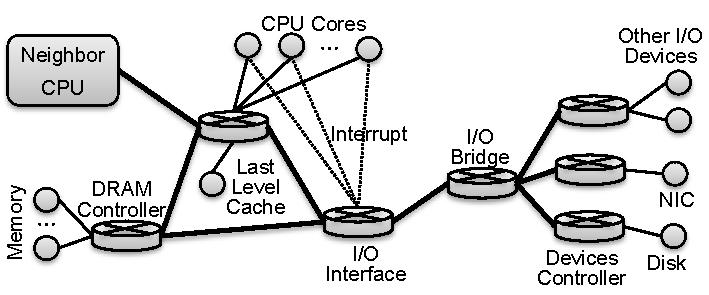
\includegraphics[height=4cm]{intro/computer-as-a-network.pdf}
  \caption[计算机内部本质是一个网络]{
    计算机内部部件之间以数据包(packet)进行通信,比如
    处理器核之间使用基于包的片上网络、
    处理器之间采用基于包的互连协议(如QPI和HT)、
    I/O设备与内存之间则通过PCI-E包进行通信。
    因此,计算机本身即可视为一个网络。}
  \label{fig:computer-as-a-network}
\end{figure}

基于以上需求,
本文提出了一种新体系结构:资源按需管理可编程的体系结构PARD\cite{pard:2015},
使数据中心服务器能够支持区分化服务,通过细粒度的硬件资源管理以及灵活的编程接口,
实现在保障关键应用服务质量的前提下提高服务器资源利用率。
PARD体系结构的核心是基于一个重要的观察:\textbf{计算机内部本质上是一个网络}。
如图\ref{fig:computer-as-a-network}所示,
CPU核、共享缓存、内存控制器、I/O设备等可以被看做是网络节点,它们之间通过包进行通信;
除了处理请求以外,这些``网络节点''与网络中的路由器/交换机具有相似的请求转发功能。
在网络领域,如何实现端到端的服务质量保障已有大量的研究,并已形成标准。
如IETF(Internet Engineering Task Force, 互联网工程任务组)于1998年提出了区分化服务
(Differentiated Services)\cite{DiffServ}的概念,
如今区分化服务已经成为应用最广泛的服务质量保障机制之一;
软件定义网络(SDN)\cite{SDN}的出现,进一步促进了网络领域服务质量保障的发展,其提出的
(1)控制平面与数据平面分离,和(2)集中控制的统一编程接口,
为网络管理带来了极大的灵活性。
本文希望能够将网络领域的区分化服务和软件定义网络的思想应用到计算机内部的网络,
用以解决数据中心当前面临的资源利用率与应用服务质量矛盾。

然而相比在计算机网络,
在体系结构这一``内部网络''中实现区分化服务与软件定义网络的功能需要面临一些额外的挑战:

首先,网络栈是整个网络中产生数据包的唯一位置,因此可以很容易的在其中增加标签机制,
实现网络流的区分。
而在计算机中有大量不同类型的硬件部件都能够向``内部网络''发送请求,
而且这些请求的类型各不相同,
如何为这些来自于不同硬件部件、类型各异的请求增加应用标签是需要解决的第一个挑战。

其次,与网络中交换机或路由器这些只进行存储转发的网络设备不同,
计算机内各个硬件部件通常包含更为复杂的功能,
如:处理器末级缓存需要为请求除完成将请求转发到下层内存控制器外,
还需要决定哪些请求数据缓存在本地,以及替换哪些数据到内存控制器;
内存控制器需要进行复杂的地址映射实现将物理地址映射到DRAM芯片,
同时还需要实现调度策略以提高访存性能;其他一些I/O设备具有更为复杂的功能。
因此如何为这些不同类型的硬件部分提供一个统一的控制平面实现对硬件资源的管理是第二个挑战。

最后,在交换机或路由器中已经为管理员提供了访问和配置其控制平面的固件接口,
而在当前的计算机中并没有类似的的固件接口。
服务器中普遍配置的IPMI/BMC\cite{ipmi}提供了诸如温度监控、电源控制、
BIOS访问等有限的监控与管理功能,利用该模块
如何实现硬件控制平面的管理,以及如何为用户(管理员)提供灵活的访问与编程接口是面临的第三个挑战。

为了解决以上三个挑战,PARD体系结构的核心设计理念可以归结为以下四点:
\textbf{1)标签机制},
通过在请求源(如处理器核或具有DMA功能的I/O设备)增加标签寄存器,使用其记录当前正在使用该部件的应用标签,
发出请求时附带该标签,并随着请求在整个计算机内部传播,实现应用区分;
\textbf{2)可编程控制平面},
为共享硬件资源的控制器增加控制平面,控制平面可根据请求标签查询规则进行区分处理,该规则可通过软件实现可编程;
\textbf{3)节点内统一资源管理},
节点内所有的控制平面通过控制平面网络连接到资源管理模块,提供对控制平面的编程接口,实现所有共享资源的统一管理;
\textbf{4)Trigger$\Rightarrow$Action编程方法},
一种基于动作触发的资源管理策略,实现资源实时监控和调整。

本文后续章节将讨论如何在现有体系结构上扩展以实现标签机制;
通用控制平面的设计以及可编程机制的实现,
并包括末级缓存控制器和内存控制器中控制平面的具体设计;
基于以上两种机制实现无Hypervisor的全硬件支持虚拟化系统,
以及如何实现资源按需分配的区分化服务,并使用模拟器对其效果进行验证。
最后在基于FPGA的原型系统中验证PARD体系结构的效果,
并讨论了原型系统实现过程中的经验与教训。


\section{本文的主要贡献}

本文的论点是:
在应用数量众多、需求多样且不断变化的数据中心场景下,计算机体系结构需要重新设计,
为应用提供区分化服务、良好的性能隔离,并具备灵活的资源管理编程接口,
实现资源使用的强控制与按需分配,
才能解决数据中心资源利用率与服务质量冲突的问题。

本文的主要贡献包括:

% 可在多个层次(虚拟机、进程、线程、API、...)区分应用,实现了NoHyper功能
第一,提出``标签化地址空间(Labeled Address Space)''概念。
正如多进程技术的出现引入了虚拟地址空间抽象,
随着虚拟化、云计算与多租户使用模式的出现,
现有的虚拟地址空间抽象无法满足多租户之间的隔离需求,
一些硬件隔离技术如EPT、I/O MMU、SR-IOV等试图在现有的体系结构下支持隔离需求,
其本质则是在虚拟地址空间外增加一层额外的地址空间,但这些技术只是在功能层面上实现了隔离,
而与性能相关的部件如共享末级缓存、内存控制器等在现有体系结构下并没有实现隔离。
本文提出的标签化地址空间抽象,使用统一标签区分不同应用,
并为计算机系统内所有请求标识应用标签,硬件不再需要通过猜测的方式区分应用,
而是通过标签机制打破目前体系结构中软硬件之间的语言鸿沟,
使得共享的硬件资源能够区分来自不同应用的请求并进行区分处理。
%可在不同层次实现应用区分,如虚拟机、进程、线程或使用API标识的数据/代码段,
%以实现不同粒度的区分化服务。
%以虚拟机粒度为例,通过标签机制以及共享硬件资源内部基于标签的划分机制,
%可将一台计算机划分为多台独立的逻辑域(Logical Domain),
%在每个逻辑域内独立运行操作系统,实现NoHyper\cite{keller_nohype:_2010}的功能。

% 表+Trigger/Action <=> 处理器方案
第二,提出硬件资源共享管理方法,为硬件资源共享提供配置、监控、反馈功能,
实现毫秒(ms)级的性能反馈。
%本文两个重要观点是:资源监控与管理结合,共享资源本地与全局协同管理结合。
实时的监控与反馈是实现细粒度资源管理的重要前提,软件监控方案无法满足实时性的需求,
在硬件上直接实现监控与反馈,提出使用通用的``控制平面''实现硬件资源的配置与监控。
在具体实现上,通过基于表的控制平面实现通用的硬件资源管理接口,
使用基于处理器的数据平面实现硬件请求的灵活控制,
为计算机系统实现硬件资源可管理提供支持。

第三,提出节点内硬件共享资源的协同管理。
控制平面构成了计算机系统内硬件资源管理的基本单元,由于硬件资源之间具有关联性,
需要进行全局统筹管理。
本文通过使用控制面网络将节点内所有的控制平面连接到集中式的资源管理模块,
对硬件共享资源进行协同管理。

以上三点贡献已在PARD的模拟器及FPGA原型系统中实现。
模拟器原型是基于gem5\cite{binkert_gem5_2011}实现的全系统时钟精确模拟器,
增加或修改了大约24,118行C++/Python代码,该模拟器以在LGPL协议下开源
\footnote{PARD-gem5模拟器开源地址https://github.com/fsg-ict/PARD-gem5}。
FPGA原型系统基于MicroBlaze系统在Xilinx VC709开发板实现并完成验证,
系统运行在133MHz频率,包含4个处理器核。
两个原型系统可以作为后续相关研究的参考平台。


\section{论文的组织}

\begin{figure}[htb]
  \centering
  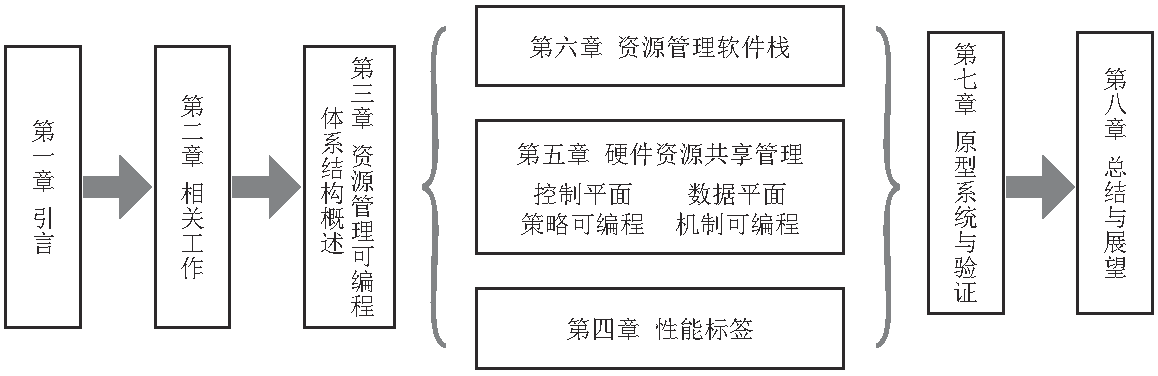
\includegraphics[width=\textwidth]{intro/thesis-structure}
  \caption{本文内容与组织结构}
  \label{fig:thesis-structure}
\end{figure}

本文共分八章,组织结构如图\ref{fig:thesis-structure}所示。

第二章介绍数据中心面临的资源利用率与服务质量冲突问题的挑战,
然后讨论现有数据中心技术的局限性,
并介绍解决该问题的现有研究。

第三章介绍PARD体系结构与关键特性,
并讨论如何利用PARD所提供的特性解决应用服务质量与资源利用率相冲突的问题。

第四章介绍PARD体系结构的基础标签化地址空间,
讨论在现有体系结构下实现标签化地址空间需要解决的关键问题,
并在模拟器上通过标签化地址空间改造,实现无软件支持的全硬件虚拟化功能。

第五章讨论硬件共享资源的管理方法,包括硬件资源的控制平面/数据平面抽象,
同时以共享末级缓存和内存控制器为例,讨论控制平面与数据平面的设计,
并通过模拟的方式验证该方案的有效性。

第六章介绍资源管理模块与资源协同管理相关的内容,包含节点内资源统一管理,
以及如何将PARD集成到现有的数据中心管理系统中(以Mesos\cite{Hindman:2011:Mesos}为例)。

第七章基于前四章的设计给出本文资源管理可编程体系结构的FPGA原型系统实现,
并对原型系统各部分功能的正确性、性能与开销进行评测。

第八章总结全文并介绍未来可能的研究工作。


% 
%%% Local Variables: 
%%% mode: latex
%%% TeX-master: t
%%% End: 

\chapter{相关研究}
\label{chap:related}

互联网应用如电子邮件、搜索、网络购物、社交网络、在线视频、网络地图等, 已经成为人们
生活的一部分。这些应用往往要为上亿用户服务,意味着互联网应用已变成如电力一样的社会
公共服务,而支撑拥有海量用户互联网应用的数据中心也成为如同发电厂一样的社会核心基础
设施。

长尾延迟(Tail Latency)问题在数据中心中受到越来越多的关注,造成长尾延迟的原因有很
多,其中最为重要的原因就是资源共享带来的干扰。
由于没有行之有效的方案对干扰进行控制,目前典型的数据中心都使用隔离的方式来减小干扰,
这一方案虽然有效缓解了长尾延迟,但它也带来了资源利用率过低的问题,
现有商用数据中心的资源利用率普遍只有10\%-30\%左右,造成极大的浪费。
如何解决服务质量与资源利用率的问题是当前业界面临的重大挑战。

本章内容安排如下:首先介绍新计算模式对数据中心的挑战,然后讨论现有数据中心技术的局
限性,即服务质量与资源利率冲突的原因,进而提出一种面向数据中心应用服务质量保障的
体系结构,最后将阐述本文的研究动机,介绍本文的主要贡献和组织结构。

%服务质量(QoS)与资源利用率是数据中心运营时需要考虑的两个重要指标,前者严重影响用户
%体验,而后者直接与数据中心的运营成本相关。然而现有的计算机体系结构并没有为服务质量
%保障提供足够的支持,造成这两个指标在现实状况下存在冲突。为了保障用户体验,在实际系
%统部署时,会更多的考虑服务质量这一指标,造成数据中心的资源利用率严重低下,普遍只有
%10\%-30\%左右。基于这一现状,本文主要讨论如何设计一种高效的数据中心体系结构,使得
%数据中心在保障应用服务质量基础上,达到较高的资源利用率。
%

\section{新计算模式对数据中心的挑战}

\subsection*{计算模式1:以云计算为基础的移动计算}

随着移动设备(平板电脑、智能手机)计算能力不断增强、成本不断降低以及无线通信技术的
快速发展,移动计算时代已经来临。如表\ref{tab:ganter-sales}所示,
Gartner调研数据显示平板电脑和手机(包含智能手机和普通手机)销量不断增加,
与此同时PC销量则不断下降。
而IDC预测到2015年智能手机销量将超过14亿部,占所有个人计算设备(包括PC、平板电脑和智能手机等)69\%的销量份额。

% Gartner关于电脑与移动设备销量的统计 
\begin{table}[htb]
  \centering
  \begin{minipage}[t]{0.9\linewidth}
  \caption[全球个人计算设备市场销量统计]{全球个人计算设备市场销量统计(单位:千部)}
  \label{tab:ganter-sales}
    \begin{tabular*}{\linewidth}{lrrrrr}
      \toprule[1.5pt]
      {\heiti 设备类型} & {\heiti 2012年} & {\heiti 2013年} & {\heiti 2014年} & {\heiti 2015年} & {\heiti 2016年} \\
      \midrule[1pt]
      PC(台式机、笔记本) &   341,273 &   296,131 &   279,000 &   259,000 &   248,000 \\ 
      超级本               &     9,787 &    21,517 &    39,000 &    62,000 &    85,000 \\ 
      平板电脑             &   120,203 &   206,807 &   216,000 &   233,000 &   259,000 \\ 
      手机                 & 1,746,177 & 1,806,964 & 1,838,000 & 1,906,000 & 1,969,000 \\ 
      其它移动设备         &       --- &     2,981 &     6,000 &     9,000 &    11,000 \\
      %总计                 & 2,217,440 & 2,334,400 & 2,378,000 & 2,470,000 & 2,572,000 \\
      \bottomrule[1.5pt]
    \end{tabular*}\\[2pt]
    \footnotesize
    数据来源:Gartner,2012年(http://www.gartner.com/newsroom/id/2610015),
    2013年(http://www.gartner.com-\\/newsroom/id/2791017),
    2014-2016年(http://www.gartner.com/newsroom/id/2954317)
  \end{minipage}
\end{table}

移动计算的快速发展带来新的计算模式:移动设备通过无线通信与运行在云计算平台的各类应
用服务进行交互。据可靠消息,目前一些主要的互联网公司(如Facebook和Baidu等)均表示,
来自移动设备的请求已占到40\%以上,并且仍在快速增长,很快将超过PC。随着4G时代的到来,
这种移动计算模式将成为未来的主流。

快速增长的移动计算需求对云计算平台的核心——数据中心带来了严峻的挑战。这种交互式计算
模式,快速的服务响应时间是衡量服务质量(Quality-of-Service,QoS)的关键指标,是让用
户满意、留住用户的关键。有研究表明,如果服务响应时间增加,公司收入就会减少。
例如,2009年微软在Bing搜索引擎上也开展实验,发现当服务响应时间增加到2000ms时,
每个用户带给企业的收益更是下降了4.3\%。由于该实验对公司产生了负面影响,最终不得不被
终止[8]。Amazon也发现其主页加载时间每增加100ms就会导致销售额下降1\% 。而Google更是
发现当搜索结果返回时间从0.4s增加到0.9s时,广告收入下降了20\%。

\begin{figure}
\begin{minipage}{0.48\textwidth}
  \centering
  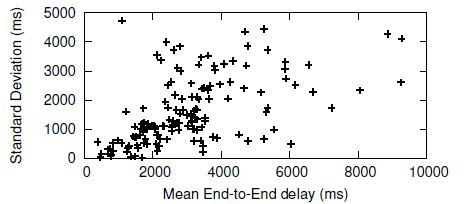
\includegraphics[height=5cm]{intro/end2end-delay}
  \caption[北美移动应用用户感知时延分布]{北美移动应用用户感知时延分布:平均延迟超过2秒且具有很大的波动性}
  \label{fig:end2end-delay}
\end{minipage}\hfill
\begin{minipage}{0.48\textwidth}
  \centering
  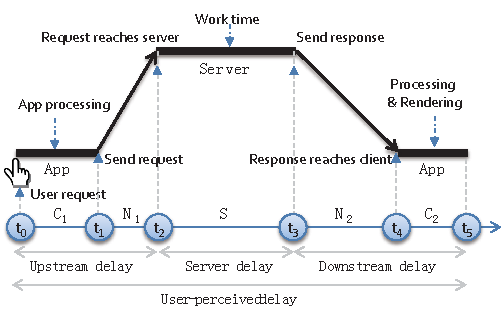
\includegraphics[height=5cm]{intro/interact-apps}
  \caption[一个典型的交互式请求的5个阶段]{一个典型的交互式请求的5个阶段:C1->N1->S->N2->C2 \cite{timecard2013}}
  \label{fig:interact-apps}
\end{minipage}
\end{figure}

移动计算的响应时间仍然存在很大的提升空间。
如图\ref{fig:end2end-delay}所示,微软公司实验数据表明在北美网络环境下,
交互式移动设备的平均时延超过2秒,而且存在较大的波动性。
图\ref{fig:interact-apps}显示典型移动交互式应用的用户请求时延分为5个阶段,
最近研究\cite{timecard2013}表明其中数据中心服务器的处理时延S约为1.2秒,占60\%。
随着4G网络的来临,数据中心将面临更大规模用户数据的处理请求。
因此,如何快速处理和及时响应移动计算请求将成为数据中心设计的核心目标之一。


\subsection*{计算模式2:面向大数据处理的实时计算}

大数据时代的到来使大数据处理架构受到越来越多的关注。2013年底中国计算机学会(CCF)
大数据专家委员会发布的《2014年大数据发展趋势十大预测》 报告中,来自学术界、产业界、
海外、跨界特邀和政府的122位专家们普遍认为,Hadoop/MapReduce框架一统天下的模式将被
打破,而实时流计算、分布式内存计算、图计算框架等将并存。

\begin{figure}[H]
  \centering
  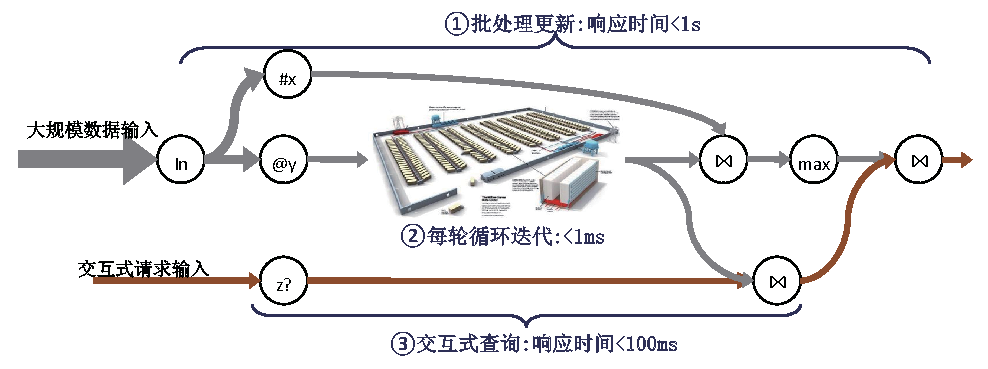
\includegraphics[height=6cm]{intro/batch-apps}
  \caption{典型的3类大数据处理需求以及相应的响应时间要求}
  \label{fig:batch-apps}
\end{figure}


大数据处理对数据中心和处理架构提出新的挑战,图\ref{fig:batch-apps}显示了典型的
大数据处理需求:首先需要支持数据的批处理更新模式(<1s);
其次数据处理会分解为多次迭代计算(<1ms);
再次还要支持实时计算模式,处理多用户的交互式查询请求(<100ms);
而这些处理所需要的数据
存放在同一个数据中心。搜索引擎是一个典型的例子,既需要对大规模网页进行内容处理,
迭代计算页面的pagerank,还需要处理大量用户的关键字查询请求。

尽管大数据处理希望能将各种处理集成在一个处理架构上,然后部署在一个数据中心。但如果
实时计算与企业营收相关,比如搜索引擎、在线购物等在线服务应用,那么正如微软Bing实验
所示,这些面向在线服务应用的实时计算的服务质量就非常关键(以下用“在线应用”
代表“实时计算”)。为了保障在线应用的服务质量,主流互联网企业一般将在线应用与大规模
批处理作业分别部署到不同的数据中心,以减少批处理作业对在线应用的干扰。但由于用户查
询请求数量具有显著的随时间变化的波动性,这种分离作业、单独部署的模式会导致在线应用
数据中心的资源平均利用率很低。如图4所示,Google的两类数据中心CPU利用率相差达2.5倍,
在线应用数据中心资源利用率仍有很大提升空间。


%% 典型的数据中心一般有5~10万台服务器组成,建设与运行维护成本往往高达几十亿人民
%% 币。然而出于保障应用服务质量的原因,现有数据中心只能维持较低的资源利用率,导致大量
%% 资源浪费。因此,本项目总体研究目标为如何设计高效通用数据中心体系结构:“通用”表
%% 示数据中心可同时运行各种不同类型应用;“高效”表示数据中心能在保障延迟敏感应用的服
%% 务质量基础上,达到较高的资源利用率(CPU利用率>60\%)。
%% 
%% 典型的数据中心一般有5~10万台中低端服务器组成,这些服务器通过内部网络互连,一起协同
%% 运行互联网应用为海量用户服务。因为这类数据中心规模很大,往往部署在大型仓库级别的机
%% 房,从应用角度来看就如同一台计算机,因此也被称为
%% “仓库级计算机(Warehouse-Scale Computer)“ \cite{WSC}。
%% 国内外著名的互联网公司往往拥有多个数据中心,服务器数量达到数十万甚
%% 至上百万台。例如,谷歌(Google)的数据中心服务器数量已经超过百万台为全球用户提供
%% 搜索、邮件、地图等服务[2];亚马逊(Amazon)仅EC2就部署了约50万台服务器提供云计算服
%% 务[3];据可靠消息,国内腾讯公司也拥有约30万服务器为用户提供各种互联网服务。
%% 
%% 尽管目前互联网企业的数据中心已经颇具规模,但一个趋势是未来数据中心还将持续发展。一
%% 方面互联网用户数量仍在不断增长,目前全球已有24亿网络用户,但很多机构预测未来全球还
%% 将新增30亿网民融入到互联网[4],这会对数据中心的数量和规模都提出更多需求。另一方面快
%% 速发展的移动终端已超越个人计算机(PC),成为终端计算设备的主流。由于移动设备性能相对
%% 较低、存储容量较小,将计算与存储转移到数据中心的需求也变得越来越强烈。因此数据中心作
%% 为基础设施也会日益重要。


\section{现有数据中心技术的局限性}

通过上述分析可知,移动计算与实时计算均对快速响应用户请求提出了强烈的需求。而当前数
据中心为了保障用户请求的服务质量,不得不通过采用牺牲资源利用率、保留过量资源的方式。
Google的数据中心技术一直处于领先地位,我们以Google为例分析数据中心资源利用率现状。
图\ref{fig:google-util-2006}显示了2006年Google数据中心平均CPU利用率为30\%左右。
但到2013年,虽然Google将数据中心分为了两类,并且批处理数据中心已经能达到75\%的CPU利用率,
但在线应用数据中心仍停留在30\%。
我们对国内企业调研发现,几大主流互联网企业在线应用数据中心CPU利用率一般都低于20\%,
有的甚至低于10\%,仍然存在很大的提升空间。

% Google数据中心利用率 
\begin{figure}
\begin{minipage}{0.57\textwidth}
  \centering
  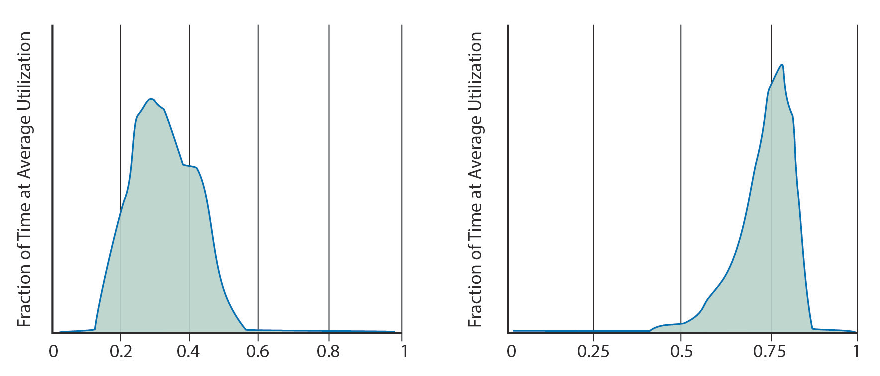
\includegraphics[height=4cm]{intro/google-util-2013}
  \caption[Google数据中心CPU利用率分布(2013年)]
    {Google数据显示2013年1至3月在线应用数据中心CPU利用率平均只有30\%(左图),
     而批处理作业数据中心则能达到75\%的利用率(两个数据中心均为2万台服务器)}
  \label{fig:google-util-2013}
\end{minipage}\hfill
\begin{minipage}{0.39\textwidth}
  \centering
  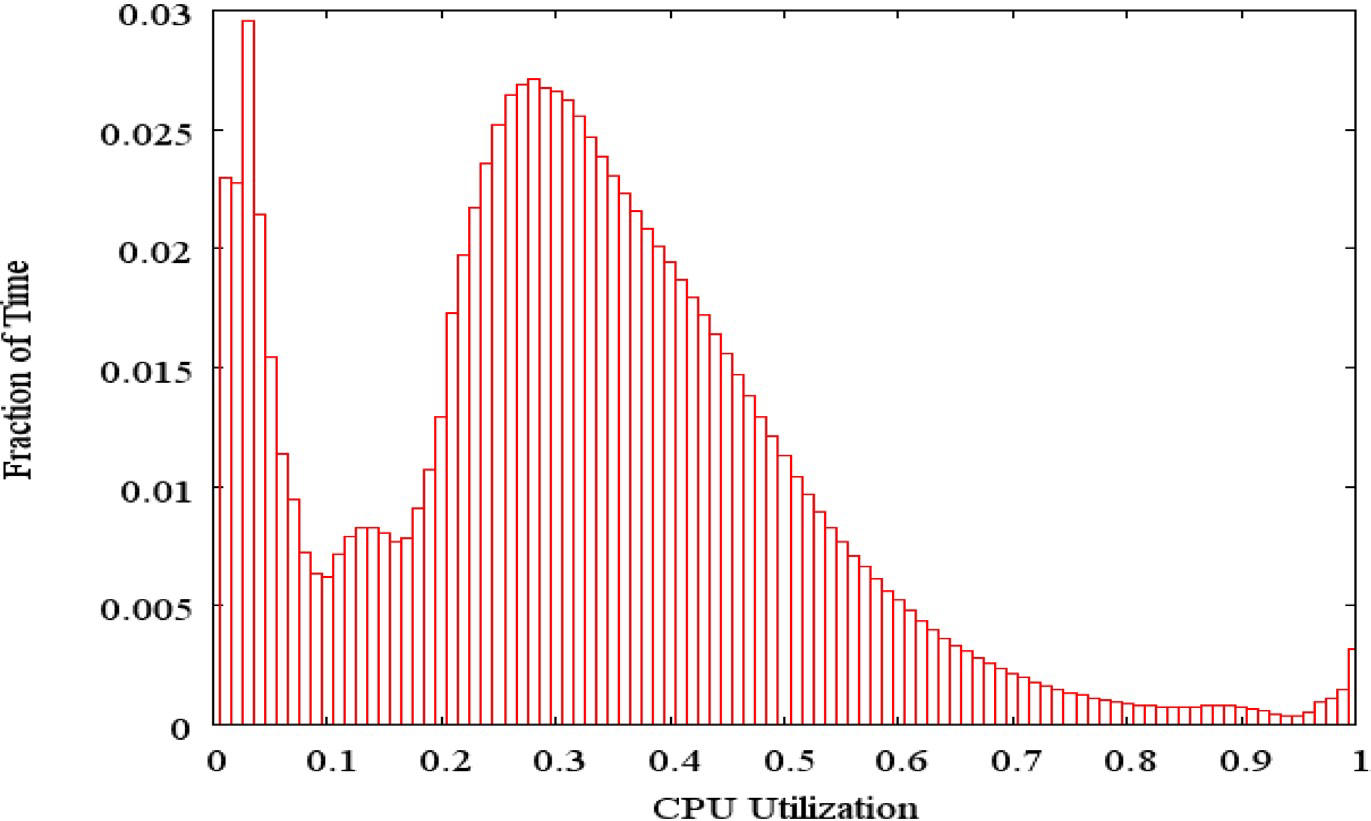
\includegraphics[height=3.5cm]{intro/google-util-2006}
  \caption[Google数据中心CPU利用率分布(2006年)]
    {Google在2006年数据中心(5000台服务器)6个月的CPU利用率分布}
  \label{fig:google-util-2006}
\end{minipage}
\end{figure}

尽管在线数据中心资源利用率只有30\%,但Google已经观察到严峻的长尾延迟现象---最慢的
1\%~10\%请求处理时间远大于所有请求的平均响应时间。
如图6所示,Google某后台服务延迟响应时间平均仅为5~6ms,但是却有相当一部分请求响应时间
超过了100ms[49]。而长尾延迟现象在数据中心环境下会被更进一步放大,因为一个用户请求需要
几百上千台服务器共同完成,只要有一台服务器的处理速度受到干扰,就会导致整个请求的处理
时间增加。Google的Jeff Dean在2012年Berkeley的报告[11]中就指出了长尾现象的严重性,假设
一台机器处理请求的平均响应时间为1ms,有1\%的请求为长尾处理时间会大于1s 
(99th-Percentile)。如果一个请求需要由100个这样的节点一起处理,那么就会出现63\%的请求
响应时间大于1s(如图7所示)。

造成在线应用数据中心资源利用率低和长尾延迟现象的核心原因是现有数据中心技术无法在多
应用混合运行时消除应用间干扰,以实现不同应用之间的性能隔离。
Google的Jeff Dean与Luiz Barroso在2013年2月的《Communication of the ACM》上撰文
“The Tail at Scale”[10]分析确认导致长尾延迟的首要原因就是资源共享,
包括体系结构层次的CPU核、Cache、访存带宽、网络带宽等,而干扰不仅来自应用,
还会来自系统软件层次的后台守护作业、监控作业、共享文件系统等。
Google在分布式架构和软件层次采用了多种缓解长尾延迟的技术,
包括操作系统容器隔离技术[12]、应用优先级管理[13]、备份请求[11]、同步后台管理进程[11]等,
取得了一定的效果,但却无法消除硬件体系结构层次上的应用之间的干扰,
导致仍然会出现图6这样的长尾延迟。

因此,现有数据中心处于“无管理的资源共享”状态,这
导致出现资源利用率与应用服务质量之间的矛盾:
一方面通过多个应用同时在数据中心部署实现资源共享能有效提高资源利用率,
但另一方面多个应用共享资源又会出现相互干扰严重影响应用的服务质量。
因此,目前企业不得不采用预留额外资源以保障延迟敏感的在线应用服务质量,
这导致很低的数据中心利用率。
而且随着多核技术的发展,单个服务器内的资源越来越多,
其上混合部署的应用数目也在不断增加,更会加剧这种矛盾。


\section{本文的研究动机}

现有数据中心技术面临资源利用率与应用服务质量的矛盾,其根本原因是大量数据中心共享资源
属于“无管理共享”状态。要实现高效通用数据中心目标,核心是从硬件上改变资源的“无
管理共享”现状以实现在体系结构上支持应用服务质量保障,在此基础上实现数据中心资源根据应
用动态管理以提高资源利用率。

回顾历史,当前数据中心面临的问题与1990年代的Internet具有相似之处。
当时流媒体、电子商务、电子邮件和FTP等大量网络应用的兴起,它们具有不同的QoS需求。
为了在IP网络中为这些应用提供端到端的服务质量保障,
互联网工程任务组(Internet Engineering Task Force, IETF)于1998年提出了区分化服务
(Differentiated Services)的概念。而如今,区分化服务已经成为应用最广泛的服务质量保障
机制之一。该技术的核心是在IP包头中定义长度为8-bit的区分化服务域,用以表示应用的
服务质量分类标识,因此路由器、交换机等网络设备便可以使用该信息对不同类别的数据包
进行区分处理,以达到区分化服务的目的。
软件定义网络(SDN)的出现,进一步促进了网络领域服务质量保障的发展,
其主要原理可以概括为:(1) 控制平面与数据平面分离;(2)集中控制的统一编程接口。

同时,计算机内部也可以被看做一个网络,如图\ref{fig:computer-as-a-network}所示,
CPU核、共享缓存、内存控制器、I/O设备等可以被看做是网络节点;除了处理请求以外,
这些“网络节点”与网络中的路由器/交换机具有相似的请求转发功能;
而它们之间也通过包进行通信,如:片内通信使用NoC包,片间通信的QPI/HT包,
以及I/O部分使用的PCI-E包。
将网络领域的区分化服务和软件定义网络的思想应用到计算机内部的网络,
用以解决数据中心当前面临的资源利用率与应用服务质量矛盾,是本文的主要研究思路与动机。

与在网络中部署SDN相比,在计算机体系结构“网络”中部署SDN会面临以下三个挑战:

首先,在整个网络栈中EndPoint是唯一的请求来源,因此SDN可以很容易的将标签机制实现在网络栈中;
与之相对的,在计算机体系结构中存在大量的硬件部件都能够发送请求,而这些请求类型又不尽相同,
因此在这样的环境下如何为请求打上标签是一个很大的挑战。

其次,在网络中所有的交换机都执行相同的存储/转发(store-and-forward)操作,但在计算机内部
不同的部件都有不同的功能,而不只是简单的存储/转发,如何为这些不同类型的部件(如末级缓存控制器、
内存控制器、I/O设备等)设计统一的控制面结构是另一个挑战。

最后,在网络交换机中已经包含了一个firmware固件用于访问和配置交换机的控制面,但计算机中却缺少
这样的firmware。现有的IPMI只被用来做有限的监控与管理功能,如对温度、风扇转速和电源控制。
因此,需要在计算机内部提供一种这样的部件实现与其它众多的控制面的通信与管理,并提供一个灵活的
编程接口对这些控制面进行操作。


%本项目总体研究目标是研究新型高效通用数据中心体系结构,能在保障应用服务质量
%的基础上将数据中心计算资源利用率提高到60\%以上。从技术挑战来看,计算机资源管理亟需新的
%具有以下特征的技术架构:
%(1)细粒度共享,有利于提高资源利用率;
%(2)性能隔离,有利于提高应用服务质量;
%(3)快速动态响应,有利于资源按需分配;
%(4)灵活协同配置,有利于协同多种资源配置以适应多种应用场景。


\section{论文的主要工作}

%本研究的目的是通过对真实环境、真实应用的访存行为特征进行更全面细致的分
%析,
%探索服务质量保障的体系结构支持,
%内存系统影响计算机整体性能的更深层次的原因,从而为体系结构、系统软件
%等的设计与优化提供一些建议。

%\begin{description}
% \item[First] \hfill \\
% The first item
% \item[Second] \hfill \\
% The second item
% \item[Third] \hfill \\
% The third etc \ldots
%\end{description}


本研究的目的是在体系结构层次解决数据中心所面临的资源利用率与服务质量相冲突的问题,
论文的主要工作围绕下述三个阶段开展:

\begin{itemize}
 \item 本研究在Xeon E5-v3平台上验证Cache容量划分功能对应用性能隔离带来的作用,
       并提出一种基于反馈模型的缓存自适应分配方法。
 \item 在体系结构内引入标签,实现应用区分,并在各个共享资源对其进行区分处理
 \item 提出一种资源管理可编程体系结构,实现可编程的硬件共享资源的细粒度管理
\end{itemize}


\section{论文的主要贡献}
In this paper, we propose Programmable Architecture for
Resourcing-on-Demand (PARD) that provides a new programming
interface to convey an application’s QoS requirements to the hardware.
PARD supports new functionalities such as fully hardwaresupported
virtualization without software hypervisors and differentiated
service (DiffServ) [60] in data center servers. For instance,
PARD can accurately isolate performance in shared data centers
to improve server utilization without degrading QoS for latencycritical
applications.



\section{论文的组织结构}

本文共分八章,第一章介绍移动计算带来的新计算模式对数据中心的挑战,然后讨论现有
数据中心技术的局限性,并针对现有体系结构提出了新的需求,最后介绍了论文的研究动机、
主要贡献和组织结构。

第二章介绍体系结构领域解决服务质量问题的现有研究,并对比以网络领域的相关内容,
讨论两者相互借鉴的可能性。

第三章对现有体系结构的服务质量支持进行评估,包括软件(cgroup, hyperviso)和硬件
两个层次。

第四章介绍资源管理可编程体系结构的概念与核心思路,并将其映射到现有体系结构,
讨论其可行性。同时应用资源管理可编程体系结构实现全硬件虚拟化,并讨论其关键技术。

第五章讨论模拟器实现,主要从功能设计角度对控制面设计,与资源管理可编程实现,
硬件支持、Trigger-Action机制,模拟的方式验证PARD的有效性。

第六章基于前两章的设计给出本文资源管理可编程体系结构的FPGA原型系统实现,
并对原型系统各部分功能的正确性、性能与开销进行了详细评测。

第七章在数据中心场景下,对本文资源管理可编程体系结构在分布式场景下应用进行讨论。

第八章总结全文并介绍未来可能的研究工作。


处理应用服务质量与资源利用率的问题,在互联网公司、芯片厂商还是学术界都在想办法解决
该问题:互联网公司方面,Baidu的Matrix项目、Google的Borg和Omega、Facebook的mesos系统
都尝试在软件架构层面解决该问题;Intel最新发布的Xeon E5-v3系列芯片,ARM芯片等都对QoS
提供了一定的支持;学术界在软硬件调度、划分方向也有大量工作。但这一问题并没有被解决,
本章首先介绍数据中心应用及其服务质量评价指标,并对现有工作进行总结,并分析其局限性。
同时参考网络领域在解决该问题的方案,

实现高效通用数据中心目标的前提在于保障应用服务质量。类似于系统安全需要所有环节安全
才能保障端到端(End-to-End)的安全,服务质量保障也需要应用全生命周期所有环节的支持。
在数据中心层面,这需要从服务器节点内部、服务器之间通信以及分布式架构多个层次协同工作。
近年来,学术界、工业界在这三个层次都不断努力。例如,近年来流行的Software Defined
Networking(SDN)技术\cite{SDN}目标就是解决数据中心网络通信的管理、共享与性能隔离问题。
Google在分布式架构上采用了超时发送备份请求同步后台管理进程等技术[11]来提高服务质量。
单节点内服务质量保障技术已成为短板。由于体系结构上不支持服务质量保障,而主流的软件
隔离技术能对资源容量隔离起到较好的效果,但无法保障性能隔离,无法保障服务质量。
总的来说,国内外在保障应用服务质量方面的研究包括单节点与分布式环境两个方面。
以下分别从这两个方面介绍相关工作。


应用混合的目标分为两方面:一是提高资源利用率,二是保障关键应用的服务质量。现有的运行时
管理方案[15]–[17]大都通过硬件性能计数器对关键应用的性能进行监控,并在性能发生下降时对非
关键应用进行各种处理,以减小由于资源竞争引起的性能问题。

造成资源利用率的核心问题在于计算机资源处于“无管理共享”状态,因此多个应用共享资源时会发
生竞争与干扰,最终导致关键应用性能不可预测。目前尚无很好的技术方案解决计算机资源“无管理
共享”的问题,以Google为代表的工业界采用将在线服务器与离线服务器分离的方法,通过降低在线
服务器的负载来保障在线应用的服务质量。

学术界在共享资源管理方面从2个维度、4个方面开展研究:软件调度、软件划分、硬件调度、硬件
划分。软件调度是通过操作系统/Hypervisor层次进行进程、线程或虚拟机级别的调度,一般调度粒
度较大,需要上下文切换,时间上也需要几毫秒到几十毫秒,不能满足在线应用的快时响应的需求;
软件划分技术能对Cache容量进行划分,但无法管理访存带宽这类资源,且软件划分技术配置调整开
销较大;硬件调度技术能支持访存请求级别的细粒度调度,但灵活性较多,不能根据不同应用按需管
理;硬件划分技术对Cache容量比较有效,但也无法对带宽等进行管理,而且同样面临灵活性差的问
题。面对诸多问题,斯坦福大学Christos Kozyrakis教授提出应该重新考虑整个计算机架构,从应用
特征、硬件隔离、操作系统、机群调度、高效资源管理硬件等多层次协同设计[18]。

\section{调度方法}
\label{sec:other}

实现高效通用数据中心目标的前提在于保障应用服务质量。类似于系统安全需要所有环节安全才能保障端到端(End-to-End)的安全,服务质量保障也需要应用全生命周期所有环节的支持。在数据中心层面,这需要从服务器节点内部、服务器之间通信以及分布式架构多个层次协同工作。近年来,学术界、工业界在这三个层次都不断努力。例如,近年来流行的Software Defined Networking(SDN)技术[15]目标就是解决数据中心网络通信的管理、共享与性能隔离问题。Google在分布式架构上采用了超时发送备份请求同步后台管理进程等技术[11]来提高服务质量。单节点内服务质量保障技术已成为短板。由于体系结构上不支持服务质量保障,而主流的软件隔离技术能对资源容量隔离起到较好的效果,但无法保障性能隔离,无法保障服务质量。

总的来说,国内外在保障应用服务质量方面的研究包括单节点与分布式环境两个方面。以下分别从这两个方面介绍相关工作。

1.2.1 单机保障服务质量研究

单机保障服务质量相关研究包括软件资源隔离技术、软硬件调度技术、硬件支持等。

软件隔离技术:针对数据中心里多个应用相互干扰的问题,一般采取虚拟化的手段在资源共享的条件下保障资源隔离,如虚拟机技术Xen[18]或Linux Container[17]。

传统虚拟机技术通过将多台虚拟机VM部署到物理机上,每台虚拟机运行一个应用或应用的一个组件,每个应用在自己的操作系统环境中独立运行,减少相互之间干扰。但这些隔离主要是资源的隔离,而无法实现性能隔离。例如为不同应用分配不同的访存带宽。而且使用虚拟机也会带来一定的性能损失[20],增加延迟,带来性能波动。

Linux Container[17]是一种轻量级虚拟化,通过在操作系统层面增添虚拟服务器功能,操作系统内核能够提供多个互相独立的用户态实例。每个用户态实例对于它自己的用户来说都像是一台独立的计算机,有自己独立的网络、文件系统、库函数和系统设置等。操作系统级虚拟化技术的优点是性能开销较小,不需要硬件的特别支持,而且能为用户态实例之间提供一定的隔离性,所以被广泛地应用在虚拟主机服务器环境中。然而,容器虚拟化技术的虚拟对象不是实际的物理资源(处理器、内存和外设),而是从用户角度出发而抽象的操作系统内部资源资,如CPU时间,内存,I/O带宽等,但如图1.5所示,Container技术对性能隔离效果并不理想。事实上,在性能隔离方面也有相关研究, Rice大学的Druschel等人[21]设计了Resource Container系统, 实现了单台物理机上多个应用间的性能隔离和CPU细粒度资源分配机制支持,然而局部隔离并不能保证全局隔离,Druschel 等人又设计了Cluster Container系统[22],以解决应用在集群范围内的隔离问题。但十几年前,单机核数目非常小,如今单节点已经有几十个核,同时运行的应用也增加了一个数量级,出现了很多新的挑战。

页着色(Page Coloring)[33]是一种以软件方式控制内存物理页映射到处理器缓存上的技术,映射到同一缓存块中的物理页对应同一颜色。基于页着色技术可以实现对共享二级缓存的划分(Partition)[36],能缓解应用在共享二级缓存上的干扰。Cho等人[34]使用Page Coloring技术来管理共享缓存。Tam等人[35]在Linux内核上实现了基于页面着色的缓存划分策略。而对于DRAM系统,也可以使用页着色技术对共享DRAM颗粒进行划分[37][39],例如,Liu等人[40]在Linux内核上实现了基于页着色的DRAM颗粒划分。北京大学李晓明教授团队也在这方面做了很多工作[41][42][43],研究利用页着色技术在虚拟环境下对共享Cache进行了划分。页着色技术能缓解一些粗粒度共享资源层次的干扰,但无法解决微体系结构的干扰,比如共享队列等,并且使用不灵活。总结而言,软件隔离技术能对资源容量隔离起到较好的效果,但无法保障性能隔离,无法保障服务质量。

软硬件调度:在多核微体系结构上,由于共享片上和片外资源的竞争会引起跨核应用之间的干扰。Jason Mars和Neil Vachharajani等人提出了竞争感知的轻量级运行时环境CAER[25],能在提高利用率的同时减少由竞争引起的跨核干扰问题。他还和Lingjia Tang等人在文章[24]还介绍了CiPE框架,可以直接用于测量和量化多核结构下应用的跨核干扰敏感度。Jason Mars等人还设计了Bubble-Up[23]机制,通过使用气泡(Bubble)来代表内存子系统的可变压力情况,能准确预测在内存子系统中竞争共享资源而导致的性能下降。Lingjia Tang等人在文章[29]提出了一种动静结合的编译方法ReQos,在确保高优先级应用的服务质量的同时让低优先级应用也可以自适应地执行。ReQoS包含一种由配置文件引导的编译技术,来识别低优先级应用中有争议的代码段。这些调度相关的工作,在具有大规模真实应用的Google“混布”数据中心里,使用该机制能在保证延迟敏感性应用的服务质量的同时,能显著提高50%~90%的资源利用率。但这些工作属于Ad-hoc类型,针对特定场景有效,并没有从根本上解决问题。

以CMU的Onur Mutlu为代表的一些学术界专家在提出了一系列调度算法[44][45][46]以缓解内存控制器的不公平问题,从而提高系统吞吐量以及服务质量。但这些算法是固化的,并不能针对某个应用进行调节,不具有灵活性。

体系结构支持:Ravi Iyer在文章[30]中提出了一种保障CMP体系结构上缓存Qos的管理框架,设计了CQos优先级分类、优先级分配和优先级执行。CQos优先级分类和优先级分配采用的是从用户到开发人员驱动的编译检测和基于流的方法;CQos优先级执行则包括(1)选择高速缓存分配、(2)动静态结合设置分区、(3)异构缓存区域。实验结果表明, CQoS在多线程或多核平台上能提高共享缓存的效率和系统性能。然而,文章[30]并没有详细描述保障CMP体系结构上缓存Qos的具体策略和软硬件支持。所以,Ravi Iyer等人又在文章[31]中实现了一种在CMP平台上保障Qos的内存体系结构,允运行时的动态资源再分配,能在减少低优先级应用性能下降的同时优化高优先级应用的性能。Andrew Herdrich等人[32]证明了用于功耗管理的基于速率(rate-based)的技术能适应于CMP结构上缓存/内存的Qos管理,其基本方法是当正在运行的低优先级任务由于资源争用而干扰了高优先级任务的性能时,就减缓核心的处理速率。通过评估时钟调制和频率缩放这两个速率限制机制,发现时钟调制更适用于缓存/内存Qos管理。

Ravi Iyer在体系结构支持服务质量方面做了一些有价值的工作,但主要集中在内存方面,并没有从整个系统角度去考虑。事实上,我们认为这个方向在未来会越来越重要,值得深入研究。
 
1.2.2 分布式环境保障服务质量

在分布式环境下,影响应用服务质量的因素主要是节点故障与干扰引起的长尾延迟,下面将从这两个方面介绍相关优化技术。

软硬件故障:Jean Dean等人设计MapReduce[26]的初衷是使用由成百上千机器组成的集群来处理超大规模的数据,所以,要求必须MapReduce能很好地处理机器故障。MapReduce采用了任务重新调度或重新执行任务(backup task)的方法来解决节点故障或短暂忙碌。比如,如果一个机器的硬盘出了问题,读取数据的速度从30M/s降低到1M/s, MapReduce框架中发送backup task机制来减少这一类长尾延迟。Backup task机制通常只会占用比正常操作多几个百分点的计算资源,但能显著改善因为故障出现的长尾延迟。不过,类似于TCP重传机制,backup task的有效性会随着负载的提高而削弱。


竞争共享资源引起的干扰:为了缓解干扰引起的长尾延迟现象,Dean等人[10]介绍了Google采用的缓解长尾延迟的技术,包括操作系统容器隔离技术[12]、应用优先级管理[13]、备份请求[11]、同步后台管理进程[11]等。R. Kapoor等人在文章[27]中提出了Chronos架构,以降低数据中心应用的长尾延迟。Chronos基于NIC上应用层数据包头字段的请求划分、应用实例负载均衡和NIC负载均衡模块的加载来消除关键通信路径上的共享资源,如内核和网络协议栈,以减少应用延迟以及相关干扰。

这些研究工作从分布式架构上一定程度上缓解了“划分/聚合”模式应用(如搜索、大数据分析等)的长尾延迟,但对“依赖/串行”模式(在线购物、社交等)应用并不显著。另一方面,随着单个服务器节点的核数目不断增加,甚至未来“片上数据中心”[47]出现,单节点内同时运行的应用也会增加,那么干扰将会越来越严重,仅仅依赖分布式架构以及软件方法将无法保障性能隔离,如何从硬件上支持服务质量保障技术将是一个值得关注与研究的方向。


\section{隔离方法}
\label{sec:multifig}

\section{软件定义网络SDN}
\label{sec:background:sdn}

The Need for a New Network Architecture % [REF] "Software-Defined Networking: The New Norm for Networks" (PDF). White paper. Open Networking Foundation. April 13, 2012. Retrieved August 22, 2013.
The explosion of mobile devices and content, server virtualization, and
advent of cloud services are among the trends driving the networking
industry to reexamine traditional network architectures. Many conventional
networks are hierarchical, built with tiers of Ethernet switches arranged in
a tree structure. This design made sense when client-server computing
was dominant, but such a static architecture is ill-suited to the dynamic
computing and storage needs of today’s enterprise data centers,
campuses, and carrier environments. Some of the key computing trends
driving the need for a new network paradigm include:


\section{本章小结}

从现有技术来看,单节点内服务质量保障技术的不足,导致节点内应用相互干扰严重,某种程
度上成为目前数据中心整体服务质量保障的短板,是成为长尾延迟现象的主要因素之一。同时
这也是一个非常具有挑战的问题,这需要跨层次协同设计。美国计算共同委员会(Computing 
Community Consortium)于2012年5月发布的计算机体系结构共同体白皮书《21世纪计算机体系
结构》中也将单节点内保障服务质量作为未来研究方向之一,其中认为[9]:“管理应用之间的相
互作用也带来了挑战。例如,这些应用如何表达服务质量(QoS)目标并且让底层的硬件、操作
系统以及虚拟层共同工作来保障它们。”


%
%
% %%% 其它部分
% \backmatter
% % 插图索引
% \listoffigures
% % 表格索引
% \listoftables
% % 公式索引
% \listofequations
%
%
% % 参考文献
% \bibliographystyle{ucasbib}
% \bibliography{ref/refs}
%
%
% % 致谢
% %%% Local Variables:
%%% mode: latex
%%% TeX-master: "../main"
%%% End:

\begin{ack}

转瞬在计算所读博的七年即将过去,这时才猛然发现,
和计算机相识已经16年了。
还记得初识时的CAI和LOGO,
还有那本似懂非懂的《数据结构:C语言描述》,
是我走上计算机道路的开始。
在这里要感谢那些给予我关怀、指导和帮助的人们。

首先要感谢我的导师孙凝晖老师,成为您的学生我的幸运。
您渊博的知识、严谨的治学态度和敏锐的思维,还有您对中国计算机事业的使命感,
是我今后学习的榜样。

还要感谢那些在重要的人生选择时给予我帮助的人:
感谢许强老师,是您将我从书本和实验带入到真正的项目,教会我需求分析、项目管理;
感谢董天正教授,是您带我进入到计算机系统结构领域;
感谢熊劲老师,您严谨的的治学态度,是我一直学习与坚持的榜样;
感谢李卓坚老师,是您手把手的教我认识机房与服务器,引领我进入系统管理的领域;
感谢马捷老师,您教会了我规范的重要。
特别要感谢包云岗老师,您是我的指路人,为我迷茫的博士路指明了方向,
也是在您的帮助下,我完成自己进入计算所时的梦想,造出了属于自己的计算机。

感谢计算所智能中心、高性能中心和先进计算机系统研究中心对我的培养。
感谢已经毕业的师兄们,
特别要感谢邢晶师兄、马灿师兄和李强师兄,是你们教会了我坚持与信念。
感谢与我共同奋斗的师弟师妹们:
感谢余子濠(濠神),我大PARD的重任就交给你了;
感谢黄博文、靳鑫,你们是我硬件入门的老师;
感谢展旭升、李宇鹏、徐天妮、姚治成、屈雨鹏、李文捷,和大家一起做科研是非常愉快的事情。
感谢张子刚,一起奋斗在博士的最后阶段,没有战友,一个人的战斗会非常的艰辛。

感谢徐志伟老师、冯晓兵老师、陈云霁老师、谢源老师、
孙广宇老师对我的学位论文提出了宝贵的修改意见。
感谢Donald E. Knuth以及Leslie Lamport,
他们开发的\TeX 和\LaTeX 使我可以专注于论文的写作。
还要感谢\ucasthesis 及其维护者xiaoyao9933,
它让我的论文写作轻松自在了许多,让我的论文格式规整漂亮了许多。

最后要感谢我的家人,感谢我的妈妈,
是您的关心与支持让我能够毫无顾虑的向着自己的理想奋斗,
您对我的爱是我一直前进的动力。

感谢我亲爱的妻子王一帆,一直默默的陪在我身边支持我、鼓励我,
是你的付出与理解,还有那些精心准备的爱心午餐,
让我能够专心科研、顺利毕业。

仅以此文,献给我的父亲。
\newline\newline

\rightline{2016年05月21日\qquad}
\rightline{于计算所\qquad\qquad}

\end{ack}

%
% % 附录
% \begin{appendix}
% %%% Local Variables: 
%%% mode: latex
%%% TeX-master: "../main"
%%% End: 

\chapter{外文资料原文}
\label{cha:engorg}
As one of the most widely used techniques in operations research, {\em
  mathematical programming} is defined as a means of maximizing a quantity known
as {\em objective function}, subject to a set of constraints represented by
equations and inequalities. Some known subtopics of mathematical programming are
linear programming, nonlinear programming, multiobjective programming, goal
programming, dynamic programming, and multilevel programming$^{[1]}$.

It is impossible to cover in a single chapter every concept of mathematical
programming. This chapter introduces only the basic concepts and techniques of
mathematical programming such that readers gain an understanding of them
throughout the book$^{[2,3]}$.


\section{Single-Objective Programming}
The general form of single-objective programming (SOP) is written
as follows,
\begin{equation}\tag*{(123)} % 如果附录中的公式不想让它出现在公式索引中,那就请
                             % 用 \tag*{xxxx}
\left\{\begin{array}{l}
\max \,\,f(x)\\[0.1 cm]
\mbox{subject to:} \\ [0.1 cm]
\qquad g_j(x)\le 0,\quad j=1,2,\cdots,p
\end{array}\right.
\end{equation}
which maximizes a real-valued function $f$ of
$x=(x_1,x_2,\cdots,x_n)$ subject to a set of constraints.

\newtheorem{mpdef}{Definition}[chapter]
\begin{mpdef}
In SOP, we call $x$ a decision vector, and
$x_1,x_2,\cdots,x_n$ decision variables. The function
$f$ is called the objective function. The set
\begin{equation}\tag*{(456)} % 这里同理,其它不再一一指定。
S=\left\{x\in\Re^n\bigm|g_j(x)\le 0,\,j=1,2,\cdots,p\right\}
\end{equation}
is called the feasible set. An element $x$ in $S$ is called a
feasible solution.
\end{mpdef}

\newtheorem{mpdefop}[mpdef]{Definition}
\begin{mpdefop}
A feasible solution $x^*$ is called the optimal
solution of SOP if and only if
\begin{equation}
f(x^*)\ge f(x)
\end{equation}
for any feasible solution $x$.
\end{mpdefop}

One of the outstanding contributions to mathematical programming was known as
the Kuhn-Tucker conditions\ref{eq:ktc}. In order to introduce them, let us give
some definitions. An inequality constraint $g_j(x)\le 0$ is said to be active at
a point $x^*$ if $g_j(x^*)=0$. A point $x^*$ satisfying $g_j(x^*)\le 0$ is said
to be regular if the gradient vectors $\nabla g_j(x)$ of all active constraints
are linearly independent.

Let $x^*$ be a regular point of the constraints of SOP and assume that all the
functions $f(x)$ and $g_j(x),j=1,2,\cdots,p$ are differentiable. If $x^*$ is a
local optimal solution, then there exist Lagrange multipliers
$\lambda_j,j=1,2,\cdots,p$ such that the following Kuhn-Tucker conditions hold,
\begin{equation}
\label{eq:ktc}
\left\{\begin{array}{l}
    \nabla f(x^*)-\sum\limits_{j=1}^p\lambda_j\nabla g_j(x^*)=0\\[0.3cm]
    \lambda_jg_j(x^*)=0,\quad j=1,2,\cdots,p\\[0.2cm]
    \lambda_j\ge 0,\quad j=1,2,\cdots,p.
\end{array}\right.
\end{equation}
If all the functions $f(x)$ and $g_j(x),j=1,2,\cdots,p$ are convex and
differentiable, and the point $x^*$ satisfies the Kuhn-Tucker conditions
(\ref{eq:ktc}), then it has been proved that the point $x^*$ is a global optimal
solution of SOP.

\subsection{Linear Programming} 
\label{sec:lp}

If the functions $f(x),g_j(x),j=1,2,\cdots,p$ are all linear, then SOP is called
a {\em linear programming}.

The feasible set of linear is always convex. A point $x$ is called an extreme
point of convex set $S$ if $x\in S$ and $x$ cannot be expressed as a convex
combination of two points in $S$. It has been shown that the optimal solution to
linear programming corresponds to an extreme point of its feasible set provided
that the feasible set $S$ is bounded. This fact is the basis of the {\em simplex
  algorithm} which was developed by Dantzig as a very efficient method for
solving linear programming.
\begin{table}[ht]
\centering
  \centering
  \caption*{Table~1\hskip1em This is an example for manually numbered table, which
    would not appear in the list of tables}
  \label{tab:badtabular2}
  \begin{tabular}[c]{|c|m{0.8in}|c|c|c|c|c|}\hline
    \multicolumn{2}{|c|}{Network Topology} & \# of nodes & 
    \multicolumn{3}{c|}{\# of clients} & Server \\\hline
    GT-ITM & Waxman Transit-Stub & 600 &
    \multirow{2}{2em}{2\%}& 
    \multirow{2}{2em}{10\%}& 
    \multirow{2}{2em}{50\%}& 
    \multirow{2}{1.2in}{Max. Connectivity}\\\cline{1-3}
    \multicolumn{2}{|c|}{Inet-2.1} & 6000 & & & &\\\hline
    \multirow{2}{1in}{Xue} & Rui  & Ni &\multicolumn{4}{c|}{\multirow{2}*{\ucasthesis}}\\\cline{2-3}
    & \multicolumn{2}{c|}{ABCDEF} &\multicolumn{4}{c|}{} \\\hline
\end{tabular}  
\end{table}

Roughly speaking, the simplex algorithm examines only the extreme points of the
feasible set, rather than all feasible points. At first, the simplex algorithm
selects an extreme point as the initial point. The successive extreme point is
selected so as to improve the objective function value. The procedure is
repeated until no improvement in objective function value can be made. The last
extreme point is the optimal solution.

\subsection{Nonlinear Programming}

If at least one of the functions $f(x),g_j(x),j=1,2,\cdots,p$ is nonlinear, then
SOP is called a {\em nonlinear programming}.

A large number of classical optimization methods have been developed to treat
special-structural nonlinear programming based on the mathematical theory
concerned with analyzing the structure of problems.
\begin{figure}[h]
  \centering
  
\includegraphics[clip]{thu-lib-logo}
  \caption*{Figure~1\hskip1em This is an example for manually numbered figure,
    which would not appear in the list of figures}
  \label{tab:badfigure2}    
\end{figure}

Now we consider a nonlinear programming which is confronted solely with
maximizing a real-valued function with domain $\Re^n$.  Whether derivatives are
available or not, the usual strategy is first to select a point in $\Re^n$ which
is thought to be the most likely place where the maximum exists. If there is no
information available on which to base such a selection, a point is chosen at
random. From this first point an attempt is made to construct a sequence of
points, each of which yields an improved objective function value over its
predecessor. The next point to be added to the sequence is chosen by analyzing
the behavior of the function at the previous points. This construction continues
until some termination criterion is met. Methods based upon this strategy are
called {\em ascent methods}, which can be classified as {\em direct methods},
{\em gradient methods}, and {\em Hessian methods} according to the information
about the behavior of objective function $f$. Direct methods require only that
the function can be evaluated at each point. Gradient methods require the
evaluation of first derivatives of $f$. Hessian methods require the evaluation
of second derivatives. In fact, there is no superior method for all
problems. The efficiency of a method is very much dependent upon the objective
function.

\subsection{Integer Programming}

{\em Integer programming} is a special mathematical programming in which all of
the variables are assumed to be only integer values. When there are not only
integer variables but also conventional continuous variables, we call it {\em
  mixed integer programming}. If all the variables are assumed either 0 or 1,
then the problem is termed a {\em zero-one programming}. Although integer
programming can be solved by an {\em exhaustive enumeration} theoretically, it
is impractical to solve realistically sized integer programming problems. The
most successful algorithm so far found to solve integer programming is called
the {\em branch-and-bound enumeration} developed by Balas (1965) and Dakin
(1965). The other technique to integer programming is the {\em cutting plane
  method} developed by Gomory (1959).

\hfill\textit{Uncertain Programming\/}\quad(\textsl{BaoDing Liu, 2006.2})

\section*{References}
\noindent{\itshape NOTE: these references are only for demonstration, they are
  not real citations in the original text.}

\begin{enumerate}[{$[$}1{$]$}]
\item Donald E. Knuth. The \TeX book. Addison-Wesley, 1984. ISBN: 0-201-13448-9
\item Paul W. Abrahams, Karl Berry and Kathryn A. Hargreaves. \TeX\ for the
  Impatient. Addison-Wesley, 1990. ISBN: 0-201-51375-7
\item David Salomon. The advanced \TeX book.  New York : Springer, 1995. ISBN:0-387-94556-3
\end{enumerate}

\chapter{外文资料的调研阅读报告或书面翻译}
\section{单目标规划}
北冥有鱼,其名为鲲。鲲之大,不知其几千里也。化而为鸟,其名为鹏。鹏之背,不知其几
千里也。怒而飞,其翼若垂天之云。是鸟也,海运则将徙于南冥。南冥者,天池也。 
\begin{equation}\tag*{(123)}
 p(y|\mathbf{x}) = \frac{p(\mathbf{x},y)}{p(\mathbf{x})}=
\frac{p(\mathbf{x}|y)p(y)}{p(\mathbf{x})}
\end{equation}

吾生也有涯,而知也无涯。以有涯随无涯,殆已!已而为知者,殆而已矣!为善无近名,为
恶无近刑,缘督以为经,可以保身,可以全生,可以养亲,可以尽年。

\subsection{线性规划}
庖丁为文惠君解牛,手之所触,肩之所倚,足之所履,膝之所倚,砉然响然,奏刀騞然,莫
不中音,合于桑林之舞,乃中经首之会。
\begin{table}[ht]
\centering
  \centering
  \caption*{表~1\hskip1em 这是手动编号但不出现在索引中的一个表格例子}
  \label{tab:badtabular3}
  \begin{tabular}[c]{|c|m{0.8in}|c|c|c|c|c|}\hline
    \multicolumn{2}{|c|}{Network Topology} & \# of nodes & 
    \multicolumn{3}{c|}{\# of clients} & Server \\\hline
    GT-ITM & Waxman Transit-Stub & 600 &
    \multirow{2}{2em}{2\%}& 
    \multirow{2}{2em}{10\%}& 
    \multirow{2}{2em}{50\%}& 
    \multirow{2}{1.2in}{Max. Connectivity}\\\cline{1-3}
    \multicolumn{2}{|c|}{Inet-2.1} & 6000 & & & &\\\hline
    \multirow{2}{1in}{Xue} & Rui  & Ni &\multicolumn{4}{c|}{\multirow{2}*{\ucasthesis}}\\\cline{2-3}
    & \multicolumn{2}{c|}{ABCDEF} &\multicolumn{4}{c|}{} \\\hline
\end{tabular}  
\end{table}

文惠君曰:“嘻,善哉!技盖至此乎?”庖丁释刀对曰:“臣之所好者道也,进乎技矣。始臣之
解牛之时,所见无非全牛者;三年之后,未尝见全牛也;方今之时,臣以神遇而不以目视,
官知止而神欲行。依乎天理,批大郤,导大窾,因其固然。技经肯綮之未尝,而况大坬乎!
良庖岁更刀,割也;族庖月更刀,折也;今臣之刀十九年矣,所解数千牛矣,而刀刃若新发
于硎。彼节者有间而刀刃者无厚,以无厚入有间,恢恢乎其于游刃必有余地矣。是以十九年
而刀刃若新发于硎。虽然,每至于族,吾见其难为,怵然为戒,视为止,行为迟,动刀甚微,
謋然已解,如土委地。提刀而立,为之而四顾,为之踌躇满志,善刀而藏之。”

文惠君曰:“善哉!吾闻庖丁之言,得养生焉。”


\subsection{非线性规划}
孔子与柳下季为友,柳下季之弟名曰盗跖。盗跖从卒九千人,横行天下,侵暴诸侯。穴室枢
户,驱人牛马,取人妇女。贪得忘亲,不顾父母兄弟,不祭先祖。所过之邑,大国守城,小
国入保,万民苦之。孔子谓柳下季曰:“夫为人父者,必能诏其子;为人兄者,必能教其弟。
若父不能诏其子,兄不能教其弟,则无贵父子兄弟之亲矣。今先生,世之才士也,弟为盗
跖,为天下害,而弗能教也,丘窃为先生羞之。丘请为先生往说之。”
\begin{figure}[h]
  \centering
  
\includegraphics{hello}
  \caption*{图~1\hskip1em 这是手动编号但不出现索引中的图片的例子}
  \label{tab:badfigure3}    
\end{figure}

柳下季曰:“先生言为人父者必能诏其子,为人兄者必能教其弟,若子不听父之诏,弟不受
兄之教,虽今先生之辩,将奈之何哉?且跖之为人也,心如涌泉,意如飘风,强足以距敌,
辩足以饰非。顺其心则喜,逆其心则怒,易辱人以言。先生必无往。”

孔子不听,颜回为驭,子贡为右,往见盗跖。

\subsection{整数规划}
盗跖乃方休卒徒大山之阳,脍人肝而餔之。孔子下车而前,见谒者曰:“鲁人孔丘,闻将军
高义,敬再拜谒者。”谒者入通。盗跖闻之大怒,目如明星,发上指冠,曰:“此夫鲁国之
巧伪人孔丘非邪?为我告之:尔作言造语,妄称文、武,冠枝木之冠,带死牛之胁,多辞缪
说,不耕而食,不织而衣,摇唇鼓舌,擅生是非,以迷天下之主,使天下学士不反其本,妄
作孝弟,而侥幸于封侯富贵者也。子之罪大极重,疾走归!不然,我将以子肝益昼餔之膳。”


\chapter{其它附录}
前面两个附录主要是给本科生做例子。其它附录的内容可以放到这里,当然如果你愿意,可
以把这部分也放到独立的文件中,然后将其 \verb|\input| 到主文件中。

% \end{appendix}
%
% % 个人简历
% \begin{resume}

\noindent
姓名:马久跃  性别:男  出生日期:1988.10.19  籍贯:辽宁\\

\noindent
2009.9 -- 现在       中国科学院计算技术所 计算机体系结构专业硕博研究生

\noindent
2005.9 -- 2009.7      东北师范大学软件学院 本科生\\

  \resumeitem{攻读博士学位期间发表的论文}
  \begin{enumerate}[leftmargin=1.5\parindent, nolistsep, label={[\arabic*]}]
    \item Jiuyue Ma, Xiufeng Sui, Ninghui Sun, Yupeng Li, Zihao Yu, Bowen Huang, Tianni Xu, Zhicheng Yao, Yu Chen, Haibin Wang, Lixin Zhang, Yungang Bao, Supporting Differentiated
    \item Jiuyue Ma, Xiufeng Sui, Yupeng Li, Zihao Yu, Bowen Huang, Yungang Bao, Supporting Differentiated Services in Datacenter Servers [C], OSDI'2014 Poster.
  \end{enumerate}

  \resumeitem{专利}
  \begin{enumerate}[leftmargin=1.5\parindent, nolistsep, label={[\arabic*]}]
    \item 马久跃,刘立坤,严得辰,李旭,基于设备能力的多终端数据同步方法和系统,申请号:201210208518.5,已授权
  \end{enumerate}

  \resumeitem{攻读博士学位期间参加的科研项目}
  \begin{enumerate}[leftmargin=1.5\parindent, nolistsep, label={[\arabic*]}]
    \item XX基金项目“共享存储机群系统的研究”(xxxxx),20xx年1月~20xx年12月
    \item 国家自然科学基金项目“共享存储机群系统中关键技术研究”(xxxxxxx),20xx年1月~20xx年12月
  \end{enumerate}

  \resumeitem{攻读博士学位期间的获奖情况}
  \begin{enumerate}[leftmargin=1.5\parindent, nolistsep, label={[\arabic*]}]
    \item 2011年被评为中国科学院``三好学生''
    \item 2012年获曙光博士奖学金
    \item 2015年获博士国家奖学金
  \end{enumerate}
\end{resume}

%
% \end{document}
% \end{example}
%
% \subsection{选项}
% \label{sec:option}
% 本模板提供了一些选项以方便使用:
% \begin{description}
% \item[master]
%   如果写硕士论文将此选项打开。
%   \begin{example}
% \documentclass[master]{ucasthesis}
%   \end{example}
%
% \item[doctor]
%   如果写博士论文将此选项打开。
%   \begin{example}
% \documentclass[doctor]{ucasthesis}
%   \end{example}
%
% \item[postdoctor]
%   如果写博士博士后出站报告将此选项打开。
%   \begin{example}
% \documentclass[postdoctor]{ucasthesis}
%   \end{example}
%
% \item[secret]
%   涉秘论文开关。配合另外两个命令 |\secretlevel| 和 |\secretyear| 分别用来指定保
%   密级别和时间。二者默认分别为\textbf{秘密}和当前年份。可以通过:
%   \cs{secretlevel}|{|绝密|}| 和 \cs{secretyear}|{|10|}| 年独立修改。
%   \begin{example}
% \documentclass[master, secret]{ucasthesis}
%   \end{example}
%
%
% \item[openany]
%   正规出版物的章节出现在奇数页,也就是右手边的页面,这就是 \texttt{openright},
%   也是 \ucasthesis 的默认选项。在这种情况下,如果前一章的最后一页也是奇数,那么
%   模板会自动生成一个纯粹的空白页,很多人不是很习惯这种方式,而且学校的格式似乎
%   更倾向于页面连续,那就是通常所说的 \texttt{openany}。{\fangsong 目前所有论文都是
%      openany。}这两个选项不用专门设置,\ucasthesis{} 会根据当前论文类型自动选
%   择。
%
%
% \item[arial]
%   使用真正的 arial 字体。此选项会装载 arial 字体宏包,如果此宏包不存在,就装
%   载Helvet。arialtoc 和 arialtitle 不受 arial 的影响。因为一般的 \TeX{} 发行都
%   没有 arial 字体,所以默认采用 Helvet,因为二者效果非常相似。如果你执着的要
%   用arial 字体,请参看:\href{http://www.mail-archive.com/ctan-ann@dante.de/msg00627.html}{Arial
%     字体}。
%
% \item[arialtoc]
%  目录项(章目录项除外)中的英文是否用 arial 字体。本选项和下一个 \textsl{arialtitle} 都不用用户
%  操心,模板都自动设置好了。
%
% \item[arialtitle]
%  章节标题中英文是否用 arial 字体(默认打开)。
% \end{description}
%
% \subsection{字体配置}
% \label{sec:font-config}
% 正确配置中文字体是使用模板的第一步。模板调用 ctex 宏包,提供如下字体使用方式:
% \begin{itemize}
%   \item 基于传统 CJK 包,使用 latex、pdflatex 编译;
%   \item 基于 xeCJK 包,使用 xelatex 编译。
% \end{itemize}
%
% 第一种方式的字体配置比较繁琐,建议使用 donated 制作的中文字体包(自
% 包含安装方法),请用户自行下载安装,此处不再赘述。本模板推荐使用第二
% 种方法,只要把所需字体放入系统字体文件夹(也可以指定自定义文件夹)即
% 可。
% 另外 Linux 系统缺少上述字体,这些用户可利用 fontname.def
% 文件配置所需字体。使用中易四种字体的配置如下:
% \begin{example}
% \ProvidesFile{fontname.def}
% \setCJKmainfont[BoldFont={SimHei},ItalicFont={KaiTi}]{SimSun}
% \setCJKsansfont{SimHei}
% \setCJKmonofont{FangSong}
% \setCJKfamilyfont{zhsong}{SimSun}
% \setCJKfamilyfont{zhhei}{SimHei}
% \setCJKfamilyfont{zhkai}{KaiTi}
% \setCJKfamilyfont{zhfs}{FangSong}
% \newcommand*{\songti}{\CJKfamily{zhsong}} % 宋体
% \newcommand*{\heiti}{\CJKfamily{zhhei}}   % 黑体
% \newcommand*{\kaishu}{\CJKfamily{zhkai}}  % 楷书
% \newcommand*{\fangsong}{\CJKfamily{zhfs}} % 仿宋
% \end{example}
%
% 对 Windows XP 来说如下,KaiTi 需要替换为 KaiTi\_GB2312,
% FangSong 需要替换为 FangSong\_GB2312。
%
% 宏包中包含了 ``zhfonts.py'' 脚本,为 Linux 用户提供一种交互式的方式
% 从系统中文字体中选择合适的六种字体,最终生成对应的 ``fontname.def''
% 文件。要使用它,只需在命令行输入该脚本的完整路径即可。
%
% 最后,用户可以通过命令
% \begin{shell}
% $ fs-list :lang=zh > zhfonts.txt
% \end{shell}
% 得到系统中现有的中文字体列表,并相应替换上述配置。
%
% \subsection{命令}
% \label{sec:command}
% 模板中的命令分为两类:一是格式控制,二是内容替换。格式控制如字体、字号、字距和
% 行距。内容替换如姓名、院系、专业、致谢等等。其中内容替换命令居多,而且主要集中
% 在封面上。首先来看格式控制命令。
%
% \subsubsection{基本控制命令}
% \label{sec:basiccom}
%
% \myentry{字体}
% \DescribeMacro{\songti}
% \DescribeMacro{\fangsong}
% \DescribeMacro{\heiti}
% \DescribeMacro{\kaishu}
% 等分别用来切换宋体、仿宋、黑体、楷体字体。
%
% \begin{example}
% {\songti 乾:元,亨,利贞}
% {\fangsong 初九,潜龙勿用}
% {\heiti 九二,见龙在田,利见大人}
% {\kaishu 九三,君子终日乾乾,夕惕若,厉,无咎}
% {\heiti 九五,飞龙在天,利见大人}
% {\songti 上九,亢龙有悔}
% \end{example}
%
% \myentry{字号}
% \DescribeMacro{\chuhao}
% 等命令定义一组字体大小,分别为:
%
% \begin{center}
% \begin{tabular}{lllll}
% \hline
% |\chuhao|&|\xiaochu|&|\yihao|&|\xiaoyi| &\\
% |\erhao|&|\xiaoer|&|\sanhao|&|\xiaosan|&\\
% |\sihao|& |\banxiaosi|&|\xiaosi|&|\dawu|&|\wuhao|\\
% |\xiaowu|&|\liuhao|&|\xiaoliu|&|\qihao|& |\bahao|\\\hline
% \end{tabular}
% \end{center}
%
% 使用方法为:\cs{command}\oarg{num},其中 |command| 为字号命令,|num| 为行距。比
% 如 |\xiaosi[1.5]| 表示选择小四字体,行距 1.5 倍。写作指南要求表格中的字体
% 是 \cs{dawu},模板已经设置好了。
%
% \begin{example}
% {\erhao 二号 \sanhao 三号 \sihao 四号  \qihao 七号}
% \end{example}
%
% \myentry{密级}
% \DescribeMacro{\secretlevel}
% \DescribeMacro{\secretyear}
% 定义秘密级别和年限:
%   \begin{example}
% \secretyear{5}
% \secretlevel{内部}
%   \end{example}
%
% \myentry{引用方式}
% \DescribeMacro{\onlinecite}

% 学校要求的参考文献引用有两种模式:(1)上标模式。比如``同样的工作有很
% 多$^{[1,2]}$\ldots''。(2)正文模式。比如``文[3] 中详细说明了\ldots''。其中上标
% 模式使用远比正文模式频繁,所以为了符合使用习惯,上标模式仍然用常规
% 的 |\cite{key}|,而 |\onlinecite{key}| 则用来生成正文模式。
%
% 关于参考文献模板推荐使用 \BibTeX{},关于中文参考文献需要额外增加一个 Entry: lang,将其设置为 \texttt{zh}
% 用来指示此参考文献为中文,以便 ucasbib.bst 处理。如:
% \begin{example}
% @INPROCEEDINGS{cnproceed,
%   author    = {王重阳 and 黄药师 and 欧阳峰 and 洪七公 and 段皇帝},
%   title     = {武林高手从入门到精通},
%   booktitle = {第~$N$~次华山论剑},
%   year      = 2006,
%   address   = {西安, 中国},
%   month     = sep,
%   lang      = "zh",
% }
%
% @ARTICLE{cnarticle,
%   AUTHOR  = "贾宝玉 and 林黛玉 and 薛宝钗 and 贾探春",
%   TITLE   = "论刘姥姥食量大如牛之现实意义",
%   JOURNAL = "红楼梦杂谈",
%   PAGES   = "260--266",
%   VOLUME  = "224",
%   YEAR    = "1800",
%   LANG    = "zh",
% }
% \end{example}
%
% \myentry{书脊}
% \DescribeMacro{\spine}
% 生成装订的书脊,为竖排格式,默认参数为论文中文题目。如果中文题目中没有英文字母,
% 那么直接调用此命令即可。否则,就要像例子里面那样做一些微调(参看模板自带
% 的 spine.tex)。下面是一个列子:
% \begin{example}
% \documentclass[master]{ucasthesis}
% \begin{document}
% \ctitle{论文中文题目}
% \cauthor{中文姓名}
% % |\spine| 命令需要上面两个变量
% \spine
%
% % 如果你的中文标题中有英文,那可以指定:
% \spine[中国科学院大学~\hspace{0.2em}\raisebox{2pt}{\LaTeX}%
% \hspace{-0.25em} 论文模板 \hspace{0.1em}\raisebox{2pt}%
% {v\version}\hspace{-0.25em}样例]
% \end{document}
% \end{example}
%
%
% \subsubsection{封面命令}
% \label{sec:titlepage}
% 下面是内容替换命令,其中以 |c| 开头的命令跟中文相关,|e| 开头则为对应的英文。
% 这部分的命令数目比较多,但实际上都相当简单,套用即可。
%
% 大多数命令的使用方法都是: \cs{command}\marg{arg},例外者将具体指出。这些命令都
% 在示例文档的 data/cover.tex 中。
%
% \myentry{论文标题}
% \DescribeMacro{\ctitle}
% \DescribeMacro{\etitle}
% \begin{example}
% \ctitle{论文中文题目}
% \etitle{Thesis English Title}
% \end{example}
%
% \myentry{作者姓名}
% \DescribeMacro{\cauthor}
% \DescribeMacro{\eauthor}
% \begin{example}
% \cauthor{中文姓名}
% \eauthor{Your name in PinYin}
% \end{example}
%
% \myentry{申请学位名称}
% \DescribeMacro{\cdegree}
% \DescribeMacro{\edegree}
% \begin{example}
% \cdegree{您要申请什么学位}
% \edegree{degree in English}
% \end{example}
%
% \myentry{院系名称}
% \DescribeMacro{\cdepartment}
% \DescribeMacro{\edepartment}
%
% \cs{cdepartment} 可以加一个可选参数,如:\cs{cdepartmentl}\oarg{精简}\marg{详
%   细},因为需要填写的空间有限,最好
% 给出一个详细和精简院系名称,如\textbf{计算机科学与技术}和\textbf{计算机}。
% \begin{example}
% \cdepartment[系名简称]{系名全称}
% \edepartment{Department}
% \end{example}
%
% \myentry{专业名称}
% \DescribeMacro{\cmajor}
% \DescribeMacro{\emajor}
% \begin{example}
% \cmajor{专业名称}
% \emajor{Major in English}
% \end{example}
%
% \DescribeMacro{\cfirstdiscipline}
% \DescribeMacro{\cseconddiscipline}
% \begin{example}
% \cfirstdiscipline{博士后一级学科}
% \cseconddiscipline{博士后二级学科}
% \end{example}
%
% \myentry{导师姓名}
% \DescribeMacro{\csupervisor}
% \DescribeMacro{\esupervisor}
% \begin{example}
% \csupervisor{导师~教授}
% \esupervisor{Supervisor}
% \end{example}
%
% \myentry{副导师姓名}
% \DescribeMacro{\cassosupervisor}
% \DescribeMacro{\eassosupervisor}
% \begin{example}
% \cassosupervisor{副导师~副教授}
% \eassosupervisor{Small Boss}
% \end{example}
%
% \myentry{联合导师}
% \DescribeMacro{\ccosupervisor}
% \DescribeMacro{\ecosupervisor}
% 硕士生联合指导教师,博士生联合导师。
% \begin{example}
% \ccosupervisor{联合导师~教授}
% \ecosupervisor{Tiny Boss}
% \end{example}
%
% \myentry{论文成文日期}
% \DescribeMacro{\cdate}
% \DescribeMacro{\edate}
% \DescribeMacro{\postdoctordate}
% 默认为当前时间,也可以自己指定。
% \begin{example}
% \cdate{中文日期}
% \edate{English Date}
% \postdoctordate{2009年7月——2011年7月} % 博士后研究起止日期
% \end{example}
%
% \myentry{博士后封面其它参数}
% \DescribeMacro{\catalognumber}
% \DescribeMacro{\udc}
% \DescribeMacro{\id}
% \begin{example}
% \catalognumber{分类号}
% \udc{udc}
% \id{编号}
% \end{example}
%
% \myentry{摘要}
% \DescribeEnv{cabstract}
% \DescribeEnv{eabstract}
% \begin{example}
% \begin{cabstract}
%  摘要请写在这里...
% \end{cabstract}
% \begin{eabstract}
%  here comes English abstract...
% \end{eabstract}
% \end{example}
%
% \myentry{关键词}
% \DescribeMacro{\ckeywords}
% \DescribeMacro{\ekeywords}
% 关键词用英文逗号分割写入相应的命令中,模板会解析各关键词并生成符合不同论文格式
% 要求的关键词格式。
% \begin{example}
% \ckeywords{关键词 1, 关键词 2}
% \ekeywords{keyword 1, key word 2}
% \end{example}
%
% \subsubsection{其它部分}
% \label{sec:otherparts}
% 论文其它主要部分命令:
%
% \myentry{符号对照表}
% \DescribeEnv{denotation}
% 主要符号表环境。简单定义的一个 list,跟 description 非常类似,使用方法参见示例
% 文件。带一个可选参数,用来指定符号列的宽度(默认为 2.5cm)。
% \begin{example}
% \begin{denotation}
%   \item[E] 能量
%   \item[m] 质量
%   \item[c] 光速
% \end{denotation}
% \end{example}
%
% 如果你觉得符号列的宽度不满意,那可以这样来调整:
% \begin{example}
% \begin{denotation}[1.5cm] % 设置为 1.5cm
%   \item[E] 能量
%   \item[m] 质量
%   \item[c] 光速
% \end{denotation}
% \end{example}
%
% \myentry{索引}
% 插图、表格和公式三个索引命令分别如下,将其插入到期望的位置即可(带星号的命令表
% 示对应的索引表不会出现在目录中):
%
% \begin{center}
% \begin{tabular}{ll}
% \hline
%   {\heiti 命令} & {\heiti 说明} \\\hline
% \cs{listoffigures} & 插图索引\\
% \cs{listoffigures*} & \\\hline
% \cs{listoftables} & 表格索引\\
% \cs{listoftables*} & \\\hline
% \cs{listofequations} & 公式索引\\
% \cs{listofequations*} & \\\hline
% \end{tabular}
% \end{center}
%
% \LaTeX{} 默认支持插图和表格索引,是通过 \cs{caption} 命令完成的,因此它们必须出
% 现在浮动环境中,否则不被计数。
%
% 有的同学不想让某个表格或者图片出现在索引里面,那么请使用命令 \cs{caption*},这
% 个命令不会给表格编号,也就是出来的只有标题文字而没有``表~xx'',``图~xx'',否则
% 索引里面序号不连续就显得不伦不类,这也是 \LaTeX{} 里星号命令默认的规则。
%
% 有这种需求的多是英文资料翻译部分,如果你觉得附录中英文原文中的表格和
% 图片显示成``表''和``图''很不协调的话,一个很好的办法还是用 \cs{caption*},参数
% 随便自己写,具体用法请参看示例文档。
%
% 如果你的确想让它编号,但又不想让它出现在索引中的话,那就自己改一改模板的代码吧,
% 我目前不打算给模板增加这种另类命令。
%
% 公式索引为本模板扩展,模板扩展了 \pkg{amsmath} 几个内部命令,使得公式编号样式和
% 自动索引功能非常方便。一般来说,你用到的所有数学环境编号都没问题了,这个可以参
% 看示例文档。如果你有个非常特殊的数学环境需要加入公式索引,那么请使
% 用 \cs{equcaption}\marg{编号}。此命令表示 equation caption,带一个参数,即显示
% 在索引中的编号。因为公式与图表不同,我们很少给一个公式附加一个标题,之所以起这
% 么个名字是因为图表就是通过 \cs{caption} 加入索引的,\cs{equcaption} 完全就是为
% 了生成公式列表,不产生什么标题。
%
% 使用方法如下。假如有一个非 equation 数学环境 mymath,只要在其中写一
% 句 \cs{equcaption} 就可以将它加入公式列表。
% \begin{example}
% \begin{mymath}
%   \label{eq:emc2}\equcaption{\ref{eq:emc2}}
%   E=mc^2
% \end{mymath}
% \end{example}
%
% 当然 mymath 正文中公式的编号需要你自己来做。
%
% 同图表一样,附录中的公式有时候也不希望它跟全文统一编号,而且不希望它出现在公式
% 索引中,目前的解决办法就是利用 \cs{tag*}\marg{公式编号} 来解决。用法很简单,此
% 处不再罗嗦,实例请参看示例文档附录 A 的前两个公式。
%
% \myentry{简历}
% \DescribeEnv{resume}\DescribeMacro{\resumeitem}
% 开启个人简历章节,包括发表文章列表等。其实就是一个 chapter。里面的每个子项目请用命令 |\resumeitem{sub title}|。
%
% 这里就不再列举例子了,请参看示例文档的 data/resume.tex。
%
% \myentry{附录}
% \DescribeEnv{appendix}
% 所有的附录都插到这里来。因为附录会更改默认的 chapter 属性,而后面的{\heiti 个人简
%   历}又需要恢复,所以实现为环境可以保证全局的属性不受影响。
% \begin{example}
% \begin{appendix}
%  %%% Local Variables: 
%%% mode: latex
%%% TeX-master: "../main"
%%% End: 

\chapter{外文资料原文}
\label{cha:engorg}
As one of the most widely used techniques in operations research, {\em
  mathematical programming} is defined as a means of maximizing a quantity known
as {\em objective function}, subject to a set of constraints represented by
equations and inequalities. Some known subtopics of mathematical programming are
linear programming, nonlinear programming, multiobjective programming, goal
programming, dynamic programming, and multilevel programming$^{[1]}$.

It is impossible to cover in a single chapter every concept of mathematical
programming. This chapter introduces only the basic concepts and techniques of
mathematical programming such that readers gain an understanding of them
throughout the book$^{[2,3]}$.


\section{Single-Objective Programming}
The general form of single-objective programming (SOP) is written
as follows,
\begin{equation}\tag*{(123)} % 如果附录中的公式不想让它出现在公式索引中,那就请
                             % 用 \tag*{xxxx}
\left\{\begin{array}{l}
\max \,\,f(x)\\[0.1 cm]
\mbox{subject to:} \\ [0.1 cm]
\qquad g_j(x)\le 0,\quad j=1,2,\cdots,p
\end{array}\right.
\end{equation}
which maximizes a real-valued function $f$ of
$x=(x_1,x_2,\cdots,x_n)$ subject to a set of constraints.

\newtheorem{mpdef}{Definition}[chapter]
\begin{mpdef}
In SOP, we call $x$ a decision vector, and
$x_1,x_2,\cdots,x_n$ decision variables. The function
$f$ is called the objective function. The set
\begin{equation}\tag*{(456)} % 这里同理,其它不再一一指定。
S=\left\{x\in\Re^n\bigm|g_j(x)\le 0,\,j=1,2,\cdots,p\right\}
\end{equation}
is called the feasible set. An element $x$ in $S$ is called a
feasible solution.
\end{mpdef}

\newtheorem{mpdefop}[mpdef]{Definition}
\begin{mpdefop}
A feasible solution $x^*$ is called the optimal
solution of SOP if and only if
\begin{equation}
f(x^*)\ge f(x)
\end{equation}
for any feasible solution $x$.
\end{mpdefop}

One of the outstanding contributions to mathematical programming was known as
the Kuhn-Tucker conditions\ref{eq:ktc}. In order to introduce them, let us give
some definitions. An inequality constraint $g_j(x)\le 0$ is said to be active at
a point $x^*$ if $g_j(x^*)=0$. A point $x^*$ satisfying $g_j(x^*)\le 0$ is said
to be regular if the gradient vectors $\nabla g_j(x)$ of all active constraints
are linearly independent.

Let $x^*$ be a regular point of the constraints of SOP and assume that all the
functions $f(x)$ and $g_j(x),j=1,2,\cdots,p$ are differentiable. If $x^*$ is a
local optimal solution, then there exist Lagrange multipliers
$\lambda_j,j=1,2,\cdots,p$ such that the following Kuhn-Tucker conditions hold,
\begin{equation}
\label{eq:ktc}
\left\{\begin{array}{l}
    \nabla f(x^*)-\sum\limits_{j=1}^p\lambda_j\nabla g_j(x^*)=0\\[0.3cm]
    \lambda_jg_j(x^*)=0,\quad j=1,2,\cdots,p\\[0.2cm]
    \lambda_j\ge 0,\quad j=1,2,\cdots,p.
\end{array}\right.
\end{equation}
If all the functions $f(x)$ and $g_j(x),j=1,2,\cdots,p$ are convex and
differentiable, and the point $x^*$ satisfies the Kuhn-Tucker conditions
(\ref{eq:ktc}), then it has been proved that the point $x^*$ is a global optimal
solution of SOP.

\subsection{Linear Programming} 
\label{sec:lp}

If the functions $f(x),g_j(x),j=1,2,\cdots,p$ are all linear, then SOP is called
a {\em linear programming}.

The feasible set of linear is always convex. A point $x$ is called an extreme
point of convex set $S$ if $x\in S$ and $x$ cannot be expressed as a convex
combination of two points in $S$. It has been shown that the optimal solution to
linear programming corresponds to an extreme point of its feasible set provided
that the feasible set $S$ is bounded. This fact is the basis of the {\em simplex
  algorithm} which was developed by Dantzig as a very efficient method for
solving linear programming.
\begin{table}[ht]
\centering
  \centering
  \caption*{Table~1\hskip1em This is an example for manually numbered table, which
    would not appear in the list of tables}
  \label{tab:badtabular2}
  \begin{tabular}[c]{|c|m{0.8in}|c|c|c|c|c|}\hline
    \multicolumn{2}{|c|}{Network Topology} & \# of nodes & 
    \multicolumn{3}{c|}{\# of clients} & Server \\\hline
    GT-ITM & Waxman Transit-Stub & 600 &
    \multirow{2}{2em}{2\%}& 
    \multirow{2}{2em}{10\%}& 
    \multirow{2}{2em}{50\%}& 
    \multirow{2}{1.2in}{Max. Connectivity}\\\cline{1-3}
    \multicolumn{2}{|c|}{Inet-2.1} & 6000 & & & &\\\hline
    \multirow{2}{1in}{Xue} & Rui  & Ni &\multicolumn{4}{c|}{\multirow{2}*{\ucasthesis}}\\\cline{2-3}
    & \multicolumn{2}{c|}{ABCDEF} &\multicolumn{4}{c|}{} \\\hline
\end{tabular}  
\end{table}

Roughly speaking, the simplex algorithm examines only the extreme points of the
feasible set, rather than all feasible points. At first, the simplex algorithm
selects an extreme point as the initial point. The successive extreme point is
selected so as to improve the objective function value. The procedure is
repeated until no improvement in objective function value can be made. The last
extreme point is the optimal solution.

\subsection{Nonlinear Programming}

If at least one of the functions $f(x),g_j(x),j=1,2,\cdots,p$ is nonlinear, then
SOP is called a {\em nonlinear programming}.

A large number of classical optimization methods have been developed to treat
special-structural nonlinear programming based on the mathematical theory
concerned with analyzing the structure of problems.
\begin{figure}[h]
  \centering
  
\includegraphics[clip]{thu-lib-logo}
  \caption*{Figure~1\hskip1em This is an example for manually numbered figure,
    which would not appear in the list of figures}
  \label{tab:badfigure2}    
\end{figure}

Now we consider a nonlinear programming which is confronted solely with
maximizing a real-valued function with domain $\Re^n$.  Whether derivatives are
available or not, the usual strategy is first to select a point in $\Re^n$ which
is thought to be the most likely place where the maximum exists. If there is no
information available on which to base such a selection, a point is chosen at
random. From this first point an attempt is made to construct a sequence of
points, each of which yields an improved objective function value over its
predecessor. The next point to be added to the sequence is chosen by analyzing
the behavior of the function at the previous points. This construction continues
until some termination criterion is met. Methods based upon this strategy are
called {\em ascent methods}, which can be classified as {\em direct methods},
{\em gradient methods}, and {\em Hessian methods} according to the information
about the behavior of objective function $f$. Direct methods require only that
the function can be evaluated at each point. Gradient methods require the
evaluation of first derivatives of $f$. Hessian methods require the evaluation
of second derivatives. In fact, there is no superior method for all
problems. The efficiency of a method is very much dependent upon the objective
function.

\subsection{Integer Programming}

{\em Integer programming} is a special mathematical programming in which all of
the variables are assumed to be only integer values. When there are not only
integer variables but also conventional continuous variables, we call it {\em
  mixed integer programming}. If all the variables are assumed either 0 or 1,
then the problem is termed a {\em zero-one programming}. Although integer
programming can be solved by an {\em exhaustive enumeration} theoretically, it
is impractical to solve realistically sized integer programming problems. The
most successful algorithm so far found to solve integer programming is called
the {\em branch-and-bound enumeration} developed by Balas (1965) and Dakin
(1965). The other technique to integer programming is the {\em cutting plane
  method} developed by Gomory (1959).

\hfill\textit{Uncertain Programming\/}\quad(\textsl{BaoDing Liu, 2006.2})

\section*{References}
\noindent{\itshape NOTE: these references are only for demonstration, they are
  not real citations in the original text.}

\begin{enumerate}[{$[$}1{$]$}]
\item Donald E. Knuth. The \TeX book. Addison-Wesley, 1984. ISBN: 0-201-13448-9
\item Paul W. Abrahams, Karl Berry and Kathryn A. Hargreaves. \TeX\ for the
  Impatient. Addison-Wesley, 1990. ISBN: 0-201-51375-7
\item David Salomon. The advanced \TeX book.  New York : Springer, 1995. ISBN:0-387-94556-3
\end{enumerate}

\chapter{外文资料的调研阅读报告或书面翻译}
\section{单目标规划}
北冥有鱼,其名为鲲。鲲之大,不知其几千里也。化而为鸟,其名为鹏。鹏之背,不知其几
千里也。怒而飞,其翼若垂天之云。是鸟也,海运则将徙于南冥。南冥者,天池也。 
\begin{equation}\tag*{(123)}
 p(y|\mathbf{x}) = \frac{p(\mathbf{x},y)}{p(\mathbf{x})}=
\frac{p(\mathbf{x}|y)p(y)}{p(\mathbf{x})}
\end{equation}

吾生也有涯,而知也无涯。以有涯随无涯,殆已!已而为知者,殆而已矣!为善无近名,为
恶无近刑,缘督以为经,可以保身,可以全生,可以养亲,可以尽年。

\subsection{线性规划}
庖丁为文惠君解牛,手之所触,肩之所倚,足之所履,膝之所倚,砉然响然,奏刀騞然,莫
不中音,合于桑林之舞,乃中经首之会。
\begin{table}[ht]
\centering
  \centering
  \caption*{表~1\hskip1em 这是手动编号但不出现在索引中的一个表格例子}
  \label{tab:badtabular3}
  \begin{tabular}[c]{|c|m{0.8in}|c|c|c|c|c|}\hline
    \multicolumn{2}{|c|}{Network Topology} & \# of nodes & 
    \multicolumn{3}{c|}{\# of clients} & Server \\\hline
    GT-ITM & Waxman Transit-Stub & 600 &
    \multirow{2}{2em}{2\%}& 
    \multirow{2}{2em}{10\%}& 
    \multirow{2}{2em}{50\%}& 
    \multirow{2}{1.2in}{Max. Connectivity}\\\cline{1-3}
    \multicolumn{2}{|c|}{Inet-2.1} & 6000 & & & &\\\hline
    \multirow{2}{1in}{Xue} & Rui  & Ni &\multicolumn{4}{c|}{\multirow{2}*{\ucasthesis}}\\\cline{2-3}
    & \multicolumn{2}{c|}{ABCDEF} &\multicolumn{4}{c|}{} \\\hline
\end{tabular}  
\end{table}

文惠君曰:“嘻,善哉!技盖至此乎?”庖丁释刀对曰:“臣之所好者道也,进乎技矣。始臣之
解牛之时,所见无非全牛者;三年之后,未尝见全牛也;方今之时,臣以神遇而不以目视,
官知止而神欲行。依乎天理,批大郤,导大窾,因其固然。技经肯綮之未尝,而况大坬乎!
良庖岁更刀,割也;族庖月更刀,折也;今臣之刀十九年矣,所解数千牛矣,而刀刃若新发
于硎。彼节者有间而刀刃者无厚,以无厚入有间,恢恢乎其于游刃必有余地矣。是以十九年
而刀刃若新发于硎。虽然,每至于族,吾见其难为,怵然为戒,视为止,行为迟,动刀甚微,
謋然已解,如土委地。提刀而立,为之而四顾,为之踌躇满志,善刀而藏之。”

文惠君曰:“善哉!吾闻庖丁之言,得养生焉。”


\subsection{非线性规划}
孔子与柳下季为友,柳下季之弟名曰盗跖。盗跖从卒九千人,横行天下,侵暴诸侯。穴室枢
户,驱人牛马,取人妇女。贪得忘亲,不顾父母兄弟,不祭先祖。所过之邑,大国守城,小
国入保,万民苦之。孔子谓柳下季曰:“夫为人父者,必能诏其子;为人兄者,必能教其弟。
若父不能诏其子,兄不能教其弟,则无贵父子兄弟之亲矣。今先生,世之才士也,弟为盗
跖,为天下害,而弗能教也,丘窃为先生羞之。丘请为先生往说之。”
\begin{figure}[h]
  \centering
  
\includegraphics{hello}
  \caption*{图~1\hskip1em 这是手动编号但不出现索引中的图片的例子}
  \label{tab:badfigure3}    
\end{figure}

柳下季曰:“先生言为人父者必能诏其子,为人兄者必能教其弟,若子不听父之诏,弟不受
兄之教,虽今先生之辩,将奈之何哉?且跖之为人也,心如涌泉,意如飘风,强足以距敌,
辩足以饰非。顺其心则喜,逆其心则怒,易辱人以言。先生必无往。”

孔子不听,颜回为驭,子贡为右,往见盗跖。

\subsection{整数规划}
盗跖乃方休卒徒大山之阳,脍人肝而餔之。孔子下车而前,见谒者曰:“鲁人孔丘,闻将军
高义,敬再拜谒者。”谒者入通。盗跖闻之大怒,目如明星,发上指冠,曰:“此夫鲁国之
巧伪人孔丘非邪?为我告之:尔作言造语,妄称文、武,冠枝木之冠,带死牛之胁,多辞缪
说,不耕而食,不织而衣,摇唇鼓舌,擅生是非,以迷天下之主,使天下学士不反其本,妄
作孝弟,而侥幸于封侯富贵者也。子之罪大极重,疾走归!不然,我将以子肝益昼餔之膳。”


\chapter{其它附录}
前面两个附录主要是给本科生做例子。其它附录的内容可以放到这里,当然如果你愿意,可
以把这部分也放到独立的文件中,然后将其 \verb|\input| 到主文件中。

%  \input{data/appendix02}
% \end{appendix}
% \end{example}
%
% \myentry{致谢声明}
% \DescribeEnv{ack}
% 把致谢做成一个环境更好一些,直接往里面写感谢的话就可以啦!下面是数学系一位同
% 学致谢里的话,拿过来做个广告,多希望每个人都能写这么一句啊!
% \begin{example}
% \begin{ack}
%   ……
%   还要特别感谢清华大学计算机系薛瑞尼同学在论文格式等方面给我的很多帮助!
%   顺便感谢下中科院计算所朝鲁同学对论文格式的修改!
% \end{ack}
% \end{example}
%
% \myentry{列表环境}
% \DescribeEnv{itemize}
% \DescribeEnv{enumerate}
% \DescribeEnv{description}
% 为了适合中文习惯,模板将这三个常用的列表环境用 \pkg{paralist} 对应的压缩环境替
% 换。一方面满足了多余空间的清楚,另一方面可以自己指定标签的样式和符号。细节请参
% 看 \pkg{paralist} 文档,此处不再赘述。
%
%
% \subsection{数学环境}
% \label{sec:math}
% \ucasthesis{} 定义了常用的数学环境:
%
% \begin{center}
% \begin{tabular}{*{7}{l}}\hline
%   axiom & theorem & definition & proposition & lemma & conjecture &\\
%   公理 & 定理 & 定义 & 命题 & 引理 & 猜想 &\\\hline
%   proof & corollary & example & exercise & assumption & remark & problem \\
%   证明 & 推论 & 例子& 练习 & 假设 & 注释 & 问题\\\hline
% \end{tabular}
% \end{center}
%
% 比如:
% \begin{example}
% \begin{definition}
% 道千乘之国,敬事而信,节用而爱人,使民以时。
% \end{definition}
% \end{example}
% 产生(自动编号):\\[5pt]
% \fbox{{\heiti 定义~1.1~~~} {道千乘之国,敬事而信,节用而爱人,使民以时。}}
%
% 列举出来的数学环境毕竟是有限的,如果想用{\heiti 胡说}这样的数学环境,那么很容易定义:
% \begin{example}
% \newtheorem{nonsense}{胡说}[chapter]
% \end{example}
%
% 然后这样使用:
% \begin{example}
% \begin{nonsense}
% 契丹武士要来中原夺武林秘笈。—— 慕容博
% \end{nonsense}
% \end{example}
% 产生(自动编号):\\[5pt]
% \fbox{{\heiti 胡说~1.1~~~} {契丹武士要来中原夺武林秘笈。\kern0.3ex\rule[0.8ex]{2em}{0.1ex}\kern0.3ex 慕容博}}
%
% \subsection{自定义以及其它}
% \label{sec:othercmd}
% 模板的配置文件 ucasthesis.cfg 中定义了很多固定词汇,一般无须修改。如果有特殊需求,
% 推荐在导言区使用 \cs{renewcommand}。当然,导言区里可以直接使用中文。
%
%
% \section{ThuThesis致谢}
% \label{sec:thanks}
% 感谢这些年来一直陪伴 ThuThesis 成长的新老同学,大家的需求是模板前
% 进的动力,大家的反馈是模板提高的机会。
% 
% 此版本加入了博士后出站报告的支持,本意为制作一个支持清华所有学位报告
% 的模板,孰料学校于近期对硕士、博士论文规范又有调整,未能及时更新,见
% 谅!
%
% 本人已于近期离开清华,虽不忍模板存此瑕疵,然精力有限,必不能如往日及
% 时升级,还望新的同学能参与或者接手,继续为大家服务。
% 
% \section{UCASThesis致谢}
% 感谢ThuThesis模板的作者,为国内学位论文模板提供了良好的实现基础。
%
% 感谢吴凯编写的GBT7714-2005N.bst,方便的解决了本模板文献格式问题。
% 
% 同时基于 ThuThesis 修改的版本 UCASThesis 离不开首批试用该模板的林健博士,
% 唐帝鑫, 杨阳师兄提出的宝贵修改意见。在此,我要特别感谢林健博士为此模板
% 精心的校对、修正所付出的辛勤汗水。没有林健博士对我的督促、帮助,
% 不会有该模板的诞生。
% 希望国科大的同学们继续完善该模板,欢迎fork, 但我更希望各分支版本能够
% 发起pull request造福更多同学。
%
% \StopEventually{\PrintChanges\PrintIndex}
% \clearpage
%
% \section{实现细节}
%
% \subsection{基本信息}
%    \begin{macrocode}
%<cls>\NeedsTeXFormat{LaTeX2e}[1999/12/01]
%<cls>\ProvidesClass{ucasthesis}
%<cfg>\ProvidesFile{ucasthesis.cfg}
%<cls|cfg>[2012/07/28 4.8dev University of Chinese Academy of Sciences Thesis Template]
%    \end{macrocode}
%
% \subsection{定义选项}
% \label{sec:defoption}
% TODO: 所有的选项用 \pkg{xkeyval} 来重构,现在的太罗唆了。
%
% 定义论文类型以及是否涉密
%    \begin{macrocode}
%<*cls>
\hyphenation{ucas-Thesis}
\def\ucasthesis{\textsc{ucasthesis}}
\def\version{4.8dev}
\newif\ifucas@master\ucas@masterfalse
\newif\ifucas@doctor\ucas@doctorfalse
\newif\ifucas@secret\ucas@secretfalse
\DeclareOption{master}{\ucas@mastertrue}
\DeclareOption{doctor}{\ucas@doctortrue}
\DeclareOption{secret}{\ucas@secrettrue}
%    \end{macrocode}
%
%
% 如果需要使用 arial 字体,请打开 [arial] 选项
%    \begin{macrocode}
\newif\ifucas@arial   %!
\DeclareOption{arial}{\ucas@arialtrue}
%    \end{macrocode}
%
% 目录中英文是否用 arial
%    \begin{macrocode}
\newif\ifucas@arialtoc
\DeclareOption{arialtoc}{\ucas@arialtoctrue}
%    \end{macrocode}
% 章节标题中的英文是否用 arial
%    \begin{macrocode}
\newif\ifucas@arialtitle
\DeclareOption{arialtitle}{\ucas@arialtitletrue}
%    \end{macrocode}
%
% noraggedbottom 选项
%    \begin{macrocode}
\newif\ifucas@raggedbottom\ucas@raggedbottomtrue
\DeclareOption{noraggedbottom}{\ucas@raggedbottomfalse}
%    \end{macrocode}
%
% 将选项传递给 ctexbook 类
%    \begin{macrocode}
\DeclareOption*{\PassOptionsToClass{\CurrentOption}{ctexbook}}
%    \end{macrocode}
%
% \cs{ExecuteOptions} 的参数之间用逗号分割,不能有空格。开始不知道,折腾了老半
% 天。
%    \begin{macrocode}
\ExecuteOptions{utf,arialtitle}%?
\ProcessOptions\relax
\RequirePackage{ifxetex}
 \ifxetex
  \LoadClass[cs4size,a4paper,openany,nocap,nofonts,UTF8]{ctexbook}
 \else
  \LoadClass[cs4size,a4paper,openany,nocap,winfonts,UTF8]{ctexbook}
\fi%    \end{macrocode}
%
% 用户至少要提供一个选项:指定论文类型。
%    \begin{macrocode}

\ifucas@master\relax\else
  \ifucas@doctor\relax\else
      \ClassError{ucasthesis}%
                   {You have to specify one of thesis options: master or doctor.}{}
  \fi
\fi

%    \end{macrocode}
%
% \subsection{装载宏包}
% \label{sec:loadpackage}
%
% 引用的宏包和相应的定义。
%    \begin{macrocode}
\RequirePackage{ifthen,calc}
%    \end{macrocode}
%
% \AmSTeX{} 宏包,用来排出更加漂亮的公式。
%    \begin{macrocode}
\RequirePackage{amsmath}
%    \end{macrocode}
%
% 用很爽的 \pkg{txfonts} 替换 \pkg{mathptmx} 宏包,同时用它自带的 typewriter 字
% 体替换 courier。必须出现在 \AmSTeX{} 之后。
%    \begin{macrocode}
\RequirePackage{txfonts}
%    \end{macrocode}
%
% 图形支持宏包。
%    \begin{macrocode}
\RequirePackage{graphicx}
%    \end{macrocode}
%
% 并排图形。\pkg{subfigure}、\pkg{subfig} 已经不再推荐,用新的 \pkg{subcaption}。
% 浮动图形和表格标题样式。\pkg{caption2} 已经不推荐使用,采用新的 \pkg{caption}。
%    \begin{macrocode}
\RequirePackage[labelformat=simple]{subcaption}
%    \end{macrocode}
%
% 为了兼容ctex 2.0+
%    \begin{macrocode}
\RequirePackage{indentfirst}
%    \end{macrocode}

% 更好的列表环境。
%    \begin{macrocode}
\RequirePackage[neverdecrease]{paralist}
\setdefaultleftmargin{3em}{2.2em}{1.87em}{1.7em}{1em}{1em}
%    \end{macrocode}
%
% raggedbottom,禁止Latex自动调整多余的页面底部空白,并保持脚注仍然在底部。
%    \begin{macrocode}
\ifucas@raggedbottom
  \RequirePackage[bottom,perpage]{footmisc}
  \raggedbottom
\else
  \RequirePackage[perpage]{footmisc}
\fi
%    \end{macrocode}
%
% 中文支持,我们使用 ctex 宏包。
%    \begin{macrocode}
\ifdefined \ctexset
\ctexset{autoindent=true}
\fi
\renewcommand{\baselinestretch}{1.0}
\RequirePackage{zhnumber}
\ifxetex
  \xeCJKsetup{AutoFakeBold=false,AutoFakeSlant=false,AllowBreakBetweenPuncts=true}
  \punctstyle{quanjiao}
  \normalspacedchars{-}
  
  \def\CJK@null{\kern\CJKnullspace\Unicode{48}{7}\kern\CJKnullspace}
  \defaultfontfeatures{Mapping=tex-text} % use TeX --
%    \end{macrocode}
% 默认采用中易的四款 (宋,黑,楷,仿宋) 免费字体。需要手工
% 修改 fontname.def 文件。缺少中文字体的 Linux 用户可以通过 fontname.def 文件定义字体。
%    \begin{macrocode}
  \ProvidesFile{fontname.def}
\setCJKmainfont[BoldFont={SimHei},ItalicFont={KaiTi}]{SimSun}
\setCJKsansfont{SimHei}
\setCJKmonofont{FangSong}
\setCJKfamilyfont{zhsong}{SimSun}
\setCJKfamilyfont{zhhei}{SimHei}
\setCJKfamilyfont{zhkai}{KaiTi}
\setCJKfamilyfont{zhfs}{FangSong}

\newcommand*{\songti}{\CJKfamily{zhsong}}
\newcommand*{\heiti}{\CJKfamily{zhhei}}
\newcommand*{\kaishu}{\CJKfamily{zhkai}}
\newcommand*{\fangsong}{\CJKfamily{zhfs}}


  \setmainfont{Times New Roman}
  \setsansfont{Arial}
  \setmonofont{Courier New}
\else
  \RequirePackage{CJKspace}
%    \end{macrocode}
% arial 字体需要单独安装,如果不使用 arial 字体,可以用 helvet 字体 |\textsf|
% 模拟,二者基本没有差别。
%    \begin{macrocode}
  \ifucas@arial
    \IfFileExists{arial.sty}%
                 {\RequirePackage{arial}}%
                 {\ClassWarning{ucasthesis}{no arial.sty availiable!}}
  \fi
\fi
%    \end{macrocode}
%
% 定理类环境宏包,其中 \pkg{amsmath} 选项用来兼容 \AmSTeX{} 的宏包
%    \begin{macrocode}
\RequirePackage[amsmath,thmmarks,hyperref]{ntheorem}
%    \end{macrocode}
%
% 表格控制
%    \begin{macrocode}
\RequirePackage{array}
\RequirePackage{longtable}
%    \end{macrocode}
%
% 使用三线表:\cs{toprule},\cs{midrule},\cs{bottomrule}。
%    \begin{macrocode}
\RequirePackage{booktabs}
%    \end{macrocode}
%
% 参考文献引用宏包。
%    \begin{macrocode}
\RequirePackage[numbers,sort&compress]{natbib}
%    \end{macrocode}
%
% 生成有书签的 pdf 及其开关,请结合 gbk2uni 避免书签乱码。
%    \begin{macrocode}
\RequirePackage{hyperref}
\ifxetex
  \hypersetup{%
    CJKbookmarks=true}
\else
  \hypersetup{%
    unicode=true,
    CJKbookmarks=false}
\fi

\RequirePackage{refcount}
\newcommand{\chapterref}[1]{%
  \@ifundefined{hyperref}{}{\hyperref[#1]%
  {\zhnumber{\getrefnumber{#1}}}}}

\RequirePackage{xcolor}
\definecolor{ucascitecolor}{rgb}{0.0, 0.50, 0.0}
\definecolor{ucaslinkcolor}{rgb}{0.75, 0.0, 0.0}
\definecolor{ucasurlcolor}{rgb}{0.0, 0.0, 0.75}
\hypersetup{%
  bookmarksnumbered=true,
  bookmarksopen=true,
  bookmarksopenlevel=1,
  breaklinks=true,
  colorlinks=true,
  citecolor=ucascitecolor,
  linkcolor=ucaslinkcolor,
  urlcolor=ucasurlcolor,
  plainpages=false,
  pdfpagelabels,
  pdfborder=0 0 0}
%    \end{macrocode}
%
% dvips 模式下网址断字有问题,请手工加载 breakurl 这个宏包解决之。
%
% 设置 url 样式,与上下文一致
%    \begin{macrocode}
\urlstyle{same}
%</cls>
%    \end{macrocode}
%
%
% \subsection{主文档格式}
% \label{sec:mainbody}
%
% \subsubsection{Three matters}
% 我们的单面和双面模式与常规的不太一样。
%    \begin{macrocode}
%<*cls>
\renewcommand\frontmatter{%
  \cleardoublepage
  \@mainmatterfalse
  \pagenumbering{Roman}
  \pagestyle{ucas@empty}}
\renewcommand\mainmatter{%
  \cleardoublepage
  \@mainmattertrue
  \pagenumbering{arabic}
  \pagestyle{ucas@headings}}
  %#\ifucas@bachelor\pagestyle{ucas@plain}\else\pagestyle{ucas@headings}\fi}
\renewcommand\backmatter{%
  \cleardoublepage
  \pagenumbering{roman}
  \pagestyle{ucas@plain}
  \@mainmattertrue}
%</cls>
%    \end{macrocode}
%
%
% \subsubsection{字体}
% \label{sec:font}
%
% 重定义字号命令
%
% Ref 1:
% \begin{verbatim}
% 参考科学出版社编写的《著译编辑手册》(1994年)
% 七号       5.25pt       1.845mm
% 六号       7.875pt      2.768mm
% 小五       9pt          3.163mm
% 五号      10.5pt        3.69mm
% 小四      12pt          4.2175mm
% 四号      13.75pt       4.83mm
% 三号      15.75pt       5.53mm
% 二号      21pt          7.38mm
% 一号      27.5pt        9.48mm
% 小初      36pt         12.65mm
% 初号      42pt         14.76mm
%
% 这里的 pt 对应的是 1/72.27 inch,也就是 TeX 中的标准 pt
% \end{verbatim}
%
% Ref 2:
% WORD 中的字号对应该关系如下:
% \begin{verbatim}
% 初号 = 42bp = 14.82mm = 42.1575pt
% 小初 = 36bp = 12.70mm = 36.135 pt
% 一号 = 26bp = 9.17mm = 26.0975pt
% 小一 = 24bp = 8.47mm = 24.09pt
% 二号 = 22bp = 7.76mm = 22.0825pt
% 小二 = 18bp = 6.35mm = 18.0675pt
% 三号 = 16bp = 5.64mm = 16.06pt
% 小三 = 15bp = 5.29mm = 15.05625pt
% 四号 = 14bp = 4.94mm = 14.0525pt
% 小四 = 12bp = 4.23mm = 12.045pt
% 五号 = 10.5bp = 3.70mm = 10.59375pt
% 小五 = 9bp = 3.18mm = 9.03375pt
% 六号 = 7.5bp = 2.56mm
% 小六 = 6.5bp = 2.29mm
% 七号 = 5.5bp = 1.94mm
% 八号 = 5bp = 1.76mm
%
% 1bp = 72.27/72 pt
% \end{verbatim}
%
% \begin{macro}{\ucas@define@fontsize}
% 根据习惯定义字号。用法:
%
% \cs{ucas@define@fontsize}\marg{字号名称}\marg{磅数}
%
% 避免了字号选择和行距的紧耦合。所有字号定义时为单倍行距,并提供选项指定行距倍数。
%    \begin{macrocode}
%<*cls>
\newlength\ucas@linespace
\newcommand{\ucas@choosefont}[2]{%
   \setlength{\ucas@linespace}{#2*\real{#1}}%
   \fontsize{#2}{\ucas@linespace}\selectfont}
\def\ucas@define@fontsize#1#2{%
  \expandafter\newcommand\csname #1\endcsname[1][\baselinestretch]{%
    \ucas@choosefont{##1}{#2}}}
%    \end{macrocode}
% \end{macro}
% \begin{macro}{\chuhao}
% \begin{macro}{\xiaochu}
% \begin{macro}{\yihao}
% \begin{macro}{\xiaoyi}
% \begin{macro}{\erhao}
% \begin{macro}{\xiaoer}
% \begin{macro}{\sanhao}
% \begin{macro}{\xiaosan}
% \begin{macro}{\sihao}
% \begin{macro}{\banxiaosi}
% \begin{macro}{\xiaosi}
% \begin{macro}{\dawu}
% \begin{macro}{\wuhao}
% \begin{macro}{\xiaowu}
% \begin{macro}{\liuhao}
% \begin{macro}{\xiaoliu}
% \begin{macro}{\qihao}
% \begin{macro}{\bahao}
%    \begin{macrocode}
\ucas@define@fontsize{chuhao}{42bp}
\ucas@define@fontsize{xiaochu}{36bp}
\ucas@define@fontsize{yihao}{26bp}
\ucas@define@fontsize{xiaoyi}{24bp}
\ucas@define@fontsize{erhao}{22bp}
\ucas@define@fontsize{xiaoer}{18bp}
\ucas@define@fontsize{sanhao}{16bp}
\ucas@define@fontsize{xiaosan}{15bp}
\ucas@define@fontsize{sihao}{14bp}
\ucas@define@fontsize{banxiaosi}{13bp}
\ucas@define@fontsize{xiaosi}{12bp}
\ucas@define@fontsize{dawu}{11bp}
\ucas@define@fontsize{wuhao}{10.5bp}
\ucas@define@fontsize{xiaowu}{9bp}
\ucas@define@fontsize{liuhao}{7.5bp}
\ucas@define@fontsize{xiaoliu}{6.5bp}
\ucas@define@fontsize{qihao}{5.5bp}
\ucas@define@fontsize{bahao}{5bp}
%    \end{macrocode}
% \end{macro}
% \end{macro}
% \end{macro}
% \end{macro}
% \end{macro}
% \end{macro}
% \end{macro}
% \end{macro}
% \end{macro}
% \end{macro}
% \end{macro}
% \end{macro}
% \end{macro}
% \end{macro}
% \end{macro}
% \end{macro}
% \end{macro}
% \end{macro}
%
% 正文小四号 (12pt) 字,行距为固定值 20 磅。
%    \begin{macrocode}
\renewcommand\normalsize{%
  \@setfontsize\normalsize{12bp}{20bp}
  \abovedisplayskip=10bp \@plus 2bp \@minus 2bp
  \abovedisplayshortskip=10bp \@plus 2bp \@minus 2bp
  \belowdisplayskip=\abovedisplayskip
  \belowdisplayshortskip=\abovedisplayshortskip}
%</cls>
%    \end{macrocode}
%
%
% \subsubsection{页面设置}
% \label{sec:layout}
% 本来这部分应该是最容易设置的,但根据格式规定出来的结果跟学校的 WORD 样例相差很
% 大,所以只能微调。
%    \begin{macrocode}
%<*cls>
\AtBeginDvi{\special{papersize=\the\paperwidth,\the\paperheight}}
\AtBeginDvi{\special{!%
      \@percentchar\@percentchar BeginPaperSize: a4
      ^^Ja4^^J\@percentchar\@percentchar EndPaperSize}}
\setlength{\textwidth}{\paperwidth}
\setlength{\textheight}{\paperheight}
\setlength\marginparwidth{0cm}
\setlength\marginparsep{0cm}
\addtolength{\textwidth}{-5cm}
\setlength{\topmargin}{1.75cm-1in}
\setlength{\oddsidemargin}{2.5cm-1in}
\setlength{\footskip}{0.6cm}
\setlength{\headsep}{0.5cm}
\addtolength{\textheight}{-5.25cm}

\setlength{\evensidemargin}{\oddsidemargin}
\setlength{\headheight}{20pt}
\setlength{\topskip}{0pt}
\setlength{\skip\footins}{15pt}
%</cls>
%    \end{macrocode}
%
% \subsubsection{页眉页脚}
% \label{sec:headerfooter}
% 新的一章从奇数页开始 (openright),所以必须保证它前面那页如果没有内容也必须
% 没有页眉页脚。(code stolen from \pkg{fancyhdr})
%    \begin{macrocode}
%<*cls>
\let\ucas@cleardoublepage\cleardoublepage
\newcommand{\ucas@clearemptydoublepage}{%
  \clearpage{\pagestyle{empty}\ucas@cleardoublepage}}
\let\cleardoublepage\ucas@clearemptydoublepage
%    \end{macrocode}
%
% 定义页眉和页脚。chapter 自动调用 thispagestyle{ucas@plain},所以要重新定义 ucas@plain。
% \begin{macro}{\ps@ucas@empty}
% \begin{macro}{\ps@ucas@plain}
% \begin{macro}{\ps@ucas@headings}
% 定义三种页眉页脚格式:
% \begin{itemize}
% \item \texttt{ucas@empty}:页眉页脚都没有
% \item \texttt{ucas@plain}:只显示页脚的页码
% \item \texttt{ucas@headings}:页眉页脚同时显示
% \end{itemize}
%    \begin{macrocode}
\def\ps@ucas@empty{%
  \let\@oddhead\@empty%
  \let\@evenhead\@empty%
  \let\@oddfoot\@empty%
  \let\@evenfoot\@empty}
\def\ps@ucas@foot{%
  \let\@oddhead\@empty%
  \let\@evenhead\@empty%
  \def\@oddfoot{\hfil\xiaowu\thepage\hfil}%
  \let\@evenfoot=\@oddfoot}
\def\ps@ucas@plain{%
  \def\@oddhead{\vbox to\headheight{%
    \hb@xt@\textwidth{\hfill\xiaowu\songti\ucas@ctitle:\leftmark\hfill}%
      \vskip2pt\hbox{\vrule width\textwidth height0.4pt depth0pt}}}
  \def\@oddfoot{\hfil\xiaowu\thepage\hfil}%
  \def\@evenhead{\vbox to\headheight{%
      \hb@xt@\textwidth{\xiaowu\songti%
       \hfill \ucas@ctitle:\leftmark \hfill}%
      \vskip2pt\hbox{\vrule width\textwidth height0.4pt depth0pt}}}
  \def\@oddfoot{\hfil\xiaowu\thepage\hfil}%
  \let\@evenfoot=\@oddfoot}
\def\ps@ucas@headings{%
  \def\@oddhead{\vbox to\headheight{%
    \hb@xt@\textwidth{\hfill\xiaowu\songti\leftmark\hfill}%
      \vskip2pt\hbox{\vrule width\textwidth height0.4pt depth0pt}}}
  \def\@evenhead{\vbox to\headheight{%
      \hb@xt@\textwidth{\xiaowu\songti%
       \hfill \headingtitle \hfill}%
      \vskip2pt\hbox{\vrule width\textwidth height0.4pt depth0pt}}}
  \def\@oddfoot{\hfil\xiaowu\thepage\hfil}
  \let\@evenfoot=\@oddfoot}

%    \end{macrocode}
% \end{macro}
% \end{macro}
% \end{macro}
%
% 其实可以直接写到 \cs{chapter} 的定义里面。
%    \begin{macrocode}
\renewcommand{\chaptermark}[1]{\@mkboth{\@chapapp\  ~~#1}{}}
%</cls>
%    \end{macrocode}
%
%
% \subsubsection{段落}
% \label{sec:paragraph}
%
% 段落之间的竖直距离
%    \begin{macrocode}
%<*cls>
\setlength{\parskip}{0pt \@plus2pt \@minus0pt}
%    \end{macrocode}
%
% 调整默认列表环境间的距离,以符合中文习惯。
% \begin{macro}{ucas@item@space}
%    \begin{macrocode}
\def\ucas@item@space{%
  \let\itemize\compactitem
  \let\enditemize\endcompactitem
  \let\enumerate\compactenum
  \let\endenumerate\endcompactenum
  \let\description\compactdesc
  \let\enddescription\endcompactdesc}
%</cls>
%    \end{macrocode}
% \end{macro}
%
%
% \subsubsection{脚注}
% \label{sec:footnote}
%
% 脚注字体:宋体小五,单倍行距。悬挂缩进 1.5 字符。标号在正文中是上标,在脚注中为
% 正体。默认情况下 \cs{@makefnmark} 显示为上标,同时为脚标和正文所用,所以如果要区
% 分,必须分别定义脚注的标号和正文的标号。
% \begin{macro}{\ucas@textcircled}
% 生成带圈的脚注数字。最多处理到 99,当然这个很容易扩展了。
%    \begin{macrocode}
%<*cls>
\def\ucas@textcircled#1{%
  \ifnum \value{#1} <10 \textcircled{\xiaoliu\arabic{#1}}
  \else\ifnum \value{#1} <100 \textcircled{\qihao\arabic{#1}}\fi
  \fi}
%    \end{macrocode}
% \end{macro}
%    \begin{macrocode}
\renewcommand{\thefootnote}{\ucas@textcircled{footnote}}
\renewcommand{\thempfootnote}{\ucas@textcircled{mpfootnote}}
\def\footnoterule{\vskip-3\p@\hrule\@width0.3\textwidth\@height0.4\p@\vskip2.6\p@}
\let\ucas@footnotesize\footnotesize
\renewcommand\footnotesize{\ucas@footnotesize\xiaowu[1.5]}
\def\@makefnmark{\textsuperscript{\hbox{\normalfont\@thefnmark}}}
\long\def\@makefntext#1{
  \bgroup
    \newbox\ucas@tempboxa
    \setbox\ucas@tempboxa\hbox{%
      \hb@xt@ 2em{\@thefnmark\hss}}
    \leftmargin\wd\ucas@tempboxa
    \rightmargin\z@
    \linewidth \columnwidth
    \advance \linewidth -\leftmargin
    \parshape \@ne \leftmargin \linewidth
    \footnotesize
    \@setpar{{\@@par}}%
    \leavevmode
    \llap{\box\ucas@tempboxa}%
    #1
  \par\egroup}
%</cls>
%    \end{macrocode}
%
%
% \subsubsection{数学相关}
% \label{sec:equation}
% 允许太长的公式断行、分页等。
%    \begin{macrocode}
%<*cls>
\allowdisplaybreaks[4]
\renewcommand\theequation{\ifnum \c@chapter>\z@ \thechapter-\fi\@arabic\c@equation}
%    \end{macrocode}
%
% 公式距前后文的距离由 4 个参数控制,参见 \cs{normalsize} 的定义。
%
% 公式改成 (1-1) 的形式。
% 同时为了让 \pkg{amsmath} 的 \cs{tag*} 命令得到正确的格式,我们必须修改这些代
% 码。\cs{make@df@tag} 是定义 \cs{tag*} 和 \cs{tag} 内部命令的。
% \cs{make@df@tag@@} 处理 \cs{tag*},我们就改它!
% \begin{verbatim}
% \def\make@df@tag{\@ifstar\make@df@tag@@\make@df@tag@@@}
% \def\make@df@tag@@#1{%
%   \gdef\df@tag{\maketag@@@{#1}\def\@currentlabel{#1}}}
% \end{verbatim}
%    \begin{macrocode}
\def\make@df@tag{\@ifstar\ucas@make@df@tag@@\make@df@tag@@@}
\def\ucas@make@df@tag@@#1{\gdef\df@tag{\ucas@maketag{#1}\def\@currentlabel{#1}}}
% redefinitation of tagform brokes eqref!
\renewcommand{\eqref}[1]{\textup{(\ref{#1})}}
\renewcommand\theequation{\ifnum \c@chapter>\z@ \thechapter-\fi\@arabic\c@equation}
%\ifucas@bachelor
%  \def\ucas@maketag#1{\maketag@@@{%
%    (\ignorespaces\text{\equationname\hskip0.5em}#1\unskip\@@italiccorr)}}
%  \def\tagform@#1{\maketag@@@{%
%    (\ignorespaces\text{\equationname\hskip0.5em}#1\unskip\@@italiccorr)\equcaption{#1}}}
%\else
\def\ucas@maketag#1{\maketag@@@{(\ignorespaces #1\unskip\@@italiccorr)}}
\def\tagform@#1{\maketag@@@{(\ignorespaces #1\unskip\@@italiccorr)\equcaption{#1}}}
%\fi
%    \end{macrocode}
% ^^A 使公式编号随着每开始新的一节而重新开始。
% ^^A \@addtoreset{eqation}{section}
%
% 解决证明环境中方块乱跑的问题。
%    \begin{macrocode}
\gdef\@endtrivlist#1{%  % from \endtrivlist
  \if@inlabel \indent\fi
  \if@newlist \@noitemerr\fi
  \ifhmode
    \ifdim\lastskip >\z@ #1\unskip \par
      \else #1\unskip \par \fi
  \fi
  \if@noparlist \else
    \ifdim\lastskip >\z@
       \@tempskipa\lastskip \vskip -\lastskip
      \advance\@tempskipa\parskip \advance\@tempskipa -\@outerparskip
      \vskip\@tempskipa
    \fi
    \@endparenv
  \fi #1}
%    \end{macrocode}
%
% 定理字样使用黑体,正文使用宋体,冒号隔开
%    \begin{macrocode}
\theorembodyfont{\kaishu }
\theoremheaderfont{\heiti }
%</cls>
%<*cfg>
%%\theoremsymbol{\ensuremath{\blacksquare}}
\theoremsymbol{\ensuremath{\square}}
\theoremstyle{plain}
%\theoremstyle{nonumberplain}
\newtheorem*{proof}{证明}
\theoremsymbol{}

\newtheorem{assumption}{假设}[chapter]
\newtheorem{definition}{定义}[chapter]
\newtheorem{proposition}{命题}[chapter]
\newtheorem{lemma}{引理}[chapter]
\newtheorem{theorem}{定理}[chapter]
\newtheorem{axiom}{公理}[chapter]
\newtheorem{corollary}{推论}[chapter]
\newtheorem{exercise}{练习}[chapter]
\newtheorem{example}{例}[chapter]
\newtheorem{remark}{注释}[chapter]
\newtheorem{problem}{问题}[chapter]
\newtheorem{conjecture}{猜想}[chapter]
%</cfg>
%    \end{macrocode}
%
% \subsubsection{浮动对象以及表格}
% \label{sec:float}
% 设置浮动对象和文字之间的距离
%    \begin{macrocode}
%<*cls>
\setlength{\floatsep}{12bp \@plus4pt \@minus1pt}
\setlength{\intextsep}{12bp \@plus4pt \@minus2pt}
\setlength{\textfloatsep}{12bp \@plus4pt \@minus2pt}
\setlength{\@fptop}{0bp \@plus1.0fil}
\setlength{\@fpsep}{12bp \@plus2.0fil}
\setlength{\@fpbot}{0bp \@plus1.0fil}
%    \end{macrocode}
%
% 下面这组命令使浮动对象的缺省值稍微宽松一点,从而防止幅度对象占据过多的文本页面,
% 也可以防止在很大空白的浮动页上放置很小的图形。
%    \begin{macrocode}
\renewcommand{\textfraction}{0.15}
\renewcommand{\topfraction}{0.85}
\renewcommand{\bottomfraction}{0.65}
\renewcommand{\floatpagefraction}{0.60}
%    \end{macrocode}
%
% 定制浮动图形和表格标题样式
% \begin{itemize}
%   \item 图表标题字体为 11pt, 这里写作大五号
%   \item 去掉图表号后面的冒号。图序与图名文字之间空一个汉字符宽度。
%   \item 图:caption 在下,段前空 6 磅,段后空 12 磅
%   \item 表:caption 在上,段前空 12 磅,段后空 6 磅
% \end{itemize}
%    \begin{macrocode}
\let\old@tabular\@tabular
\def\ucas@tabular{\dawu[1.5]\old@tabular}
\DeclareCaptionLabelFormat{ucas}{{\dawu[1.5]\songti #1~\rmfamily #2}}
\DeclareCaptionLabelSeparator{ucas}{\hspace{1em}}
\DeclareCaptionFont{ucas}{\dawu[1.5]}
\captionsetup{labelformat=ucas,labelsep=ucas,font=ucas}
\captionsetup[table]{position=top,belowskip={12bp-\intextsep},aboveskip=6bp}
\captionsetup[figure]{position=bottom,belowskip={12bp-\intextsep},aboveskip=6bp}
\captionsetup[sub]{font=ucas,skip=6bp}
\renewcommand{\thesubfigure}{(\alph{subfigure})}
\renewcommand{\thesubtable}{(\alph{subtable})}
% \renewcommand{\p@subfigure}{:}
%    \end{macrocode}
% 我们采用 \pkg{longtable} 来处理跨页的表格。同样我们需要设置其默认字体为五号。
%    \begin{macrocode}
\let\ucas@LT@array\LT@array
\def\LT@array{\dawu[1.5]\ucas@LT@array} % set default font size
%    \end{macrocode}
%
% \begin{macro}{\hlinewd}
% 简单的表格使用三线表推荐用 \cs{hlinewd}。如果表格比较复杂还是用 \pkg{booktabs} 的命
% 令好一些。
%    \begin{macrocode}
\def\hlinewd#1{%
  \noalign{\ifnum0=`}\fi\hrule \@height #1 \futurelet
    \reserved@a\@xhline}
%</cls>
%    \end{macrocode}
% \end{macro}
%
%
% \subsubsection{中文标题定义}
% \label{sec:theor}
%    \begin{macrocode}
%<*cfg>
\renewcommand\contentsname{目\hspace{1em}录}
\newcommand\scontentsname{目录}
\renewcommand\listfigurename{图目录}
\renewcommand\listtablename{表目录}
\newcommand\listequationname{公式索引}
\newcommand\equationname{公式}
\renewcommand\bibname{参考文献}
\renewcommand\indexname{索引}
\renewcommand\figurename{图}
\renewcommand\tablename{表}
\newcommand\CJKprepartname{第}
\newcommand\CJKpartname{部分}
\CTEXnumber{\ucas@thepart}{\@arabic\c@part}
\newcommand\CJKthepart{\ucas@thepart}
\newcommand\CJKprechaptername{第}
\newcommand\CJKchaptername{章}

\newcommand\CJKthechapter{\zhnumber{\@arabic\c@chapter}}
\renewcommand\chaptername{\CJKprechaptername\CJKthechapter\CJKchaptername}
\renewcommand\appendixname{附录}
\newcommand{\cabstractname}{摘\hspace{1em}要}
\newcommand{\csabstractname}{摘要}
\newcommand{\eabstractname}{Abstract}


\let\CJK@todaysave=\today
\def\CJK@todaysmall@short{\the\year 年 \the\month 月}
\def\CJK@todaysmall{\CJK@todaysmall@short \the\day 日}
\CTEXdigits{\ucas@CJK@year}{\the\year}
\CTEXnumber{\ucas@CJK@month}{\the\month}
\CTEXnumber{\ucas@CJK@day}{\the\day}
\def\CJK@todaybig@short{\ucas@CJK@year{}年\ucas@CJK@month{}月}
\def\CJK@todaybig{\CJK@todaybig@short{}\ucas@CJK@day{}日}
\def\CJK@today{\CJK@todaysmall}
\renewcommand\today{\CJK@today}
\newcommand\CJKtoday[1][1]{%
  \ifcase#1\def\CJK@today{\CJK@todaysave}
    \or\def\CJK@today{\CJK@todaysmall}
    \or\def\CJK@today{\CJK@todaybig}
  \fi}
%</cfg>
%    \end{macrocode}
%
%
% \subsubsection{章节标题}
% \label{sec:titleandtoc}
% 如果章节题目中的英文要使用 arial,那么就加上 \cs{sffamily}
%    \begin{macrocode}
%<*cls>
\ifucas@arialtitle
  \def\ucas@title@font{\sffamily}
\fi
%    \end{macrocode}
%
% \begin{macro}{\chapter}
% 章序号与章名之间空一个汉字符 黑体四号字,居中书写,单倍行距,段前空 24 磅,段
% 后空 18 磅。
%
%    \begin{macrocode}
\renewcommand\chapter{%
  \cleardoublepage%
  \thispagestyle{ucas@foot}%
  \global\@topnum\z@%
  \@afterindenttrue%
  \secdef\@chapter\@schapter}
\def\@chapter[#1]#2{%
  \ifnum \c@secnumdepth >\m@ne
   \if@mainmatter
     \refstepcounter{chapter}%
     \addcontentsline{toc}{chapter}{\protect\numberline{\@chapapp}#1}%TODO: shit
   \else
     \addcontentsline{toc}{chapter}{#1}%
   \fi
  \else
    \addcontentsline{toc}{chapter}{#1}%
  \fi
  \chaptermark{#1}%
  \@makechapterhead{#2}}
\def\@makechapterhead#1{%
  \vspace*{17bp}
  {\parindent \z@ \centering
    \csname ucas@title@font\endcsname\heiti\sihao[2.41]
    \ifnum \c@secnumdepth >\m@ne
      \@chapapp\hskip1em
    \fi
    #1\par\nobreak
    \vskip 16.5bp}}
\def\@schapter#1{%
  \@makeschapterhead{#1}
  \@afterheading}
\def\@makeschapterhead#1{%
  \vspace*{17bp}%
  {\parindent \z@ \centering
   \csname ucas@title@font\endcsname\heiti\sihao[2.41]
     \def\@tempa{#1}
     \def\@tempb{\eabstractname}
     \ifx\@tempa\@tempb\fi

   \interlinepenalty\@M
   #1\par\nobreak
    \vskip 16.5bp}}
%    \end{macrocode}
% \end{macro}
%
% \begin{macro}{\ucas@chapter*}
%
% \cs{ucas@chapter*}\oarg{tocline}\marg{title}\oarg{header}: tocline 是出现在目录
% 中的条目,如果为空则此 chapter 不出现在目录中,如果省略表示目录出现 title;
% title 是章标题;header 是页眉出现的标题,如果忽略则取 title。通过这个宏我才真
% 正体会到 \TeX{} macro 的力量!
%    \begin{macrocode}
\newcounter{ucas@bookmark}
\def\ucas@chapter*{%
  \@ifnextchar [ % ]
    {\ucas@@chapter}
    {\ucas@@chapter@}}
\def\ucas@@chapter@#1{\ucas@@chapter[#1]{#1}}
\def\ucas@@chapter[#1]#2{%
  \@ifnextchar [ % ]
    {\ucas@@@chapter[#1]{#2}}
    {\ucas@@@chapter[#1]{#2}[]}}
\def\ucas@@@chapter[#1]#2[#3]{%
  \cleardoublepage
  \phantomsection
  \def\@tmpa{#1}
  \def\@tmpb{#3}
  \ifx\@tmpa\@empty
    \ifx\@tmpb\@empty
      \addtocounter{ucas@bookmark}\@ne
      \pdfbookmark[0]{#2}{ucaschapter.\theucas@bookmark}
    \else
      \addtocounter{ucas@bookmark}\@ne
      \pdfbookmark[0]{#3}{ucaschapter.\theucas@bookmark}
    \fi
  \else
    \addcontentsline{toc}{chapter}{#1}
  \fi
  \chapter*{#2}
  \ifx\@tmpb\@empty
    \@mkboth{#2}{#2}
  \else
    \@mkboth{#3}{#3}
  \fi}
%    \end{macrocode}
% \end{macro}
% \begin{macro}{\section}
% 一级节标题,例如:2.1  实验装置与实验方法
% 节标题序号与标题名之间空一个汉字符(下同)。
% 采用黑体小四字居左书写,行距为1.75倍行距,段前空 8 磅,段后空 8 磅。
%
%    \begin{macrocode}
\renewcommand\section{\@startsection {section}{1}{\z@}%
                     {8bp\@plus 1ex \@minus .2ex}%
                     {8bp \@plus .2ex}%
                     {\csname ucas@title@font\endcsname\heiti\xiaosi[1.75]}}
%    \end{macrocode}
% \end{macro}
%
% \begin{macro}{\subsection}
% 二级节标题,例如:2.1.1 实验装置
%    \begin{macrocode}
\renewcommand\subsection{\@startsection{subsection}{2}{\z@}%
                        {4bp\@plus 1ex \@minus .2ex}%
                        {4bp \@plus .2ex}%
                        {\csname ucas@title@font\endcsname\heiti\xiaosi[1.75]}}
%    \end{macrocode}
% \end{macro}
%
% \begin{macro}{\subsubsection}
% 三级节标题,例如: 2.1.2.1 归纳法
% 采用黑体小四号(12pt)字居左书写,行距为1.75倍,段前空 4 磅,段后空 4 磅。
%    \begin{macrocode}
\renewcommand\subsubsection{\@startsection{subsubsection}{3}{\z@}%
                           {4bp\@plus 1ex \@minus .2ex}%
                           {4bp \@plus .2ex}%
                           {\csname ucas@title@font\endcsname\heiti\xiaosi[1.75]}}
%</cls>
%    \end{macrocode}
% \end{macro}
%
%
% \subsubsection{目录格式}
% \label{sec:toc}
% 最多涉及 4 层,即: x.x.x.x。\par
% chapter(0), section(1), subsection(2), subsubsection(3)
%    \begin{macrocode}
%<*cls>

\setcounter{secnumdepth}{3}
\setcounter{tocdepth}{2}

%    \end{macrocode}
%
% 每章标题行前空 6 磅,后空 0 磅。如果使用目录项中英文要使用 Arial,那么就加上 \cs{sffamily}。
% 章节名中英文用 Arial 字体,页码仍用 Times。
% \begin{macro}{\tableofcontents}
%   目录生成命令。
%    \begin{macrocode}
\renewcommand\tableofcontents{%
  \cleardoublepage
  \ucas@chapter*{\contentsname}[\scontentsname]
  \xiaosi[1.5]\@starttoc{toc}\normalsize}
\ifucas@arialtoc
  \def\ucas@toc@font{\sffamily}
\fi
\def\@pnumwidth{2em} % 这个参数没用了
\def\@tocrmarg{2em}
\def\@dotsep{1} % 目录点间的距离
\def\@dottedtocline#1#2#3#4#5{%
  \ifnum #1>\c@tocdepth \else
    \vskip \z@ \@plus.2\p@
    {\leftskip #2\relax \rightskip \@tocrmarg \parfillskip -\rightskip
    \parindent #2\relax\@afterindenttrue
    \interlinepenalty\@M
    \leavevmode
    \@tempdima #3\relax
    \advance\leftskip \@tempdima \null\nobreak\hskip -\leftskip
    {\csname ucas@toc@font\endcsname #4}\nobreak
    \leaders\hbox{$\m@th\mkern \@dotsep mu\hbox{.}\mkern \@dotsep mu$}\hfill
    \nobreak{\normalfont \normalcolor #5}%
    \par\penalty\@highpenalty}%
  \fi}
\renewcommand*\l@chapter[2]{%
  \ifnum \c@tocdepth >\m@ne
    \addpenalty{-\@highpenalty}%
    \vskip 8bp \@plus\p@
    \setlength\@tempdima{4em}%
    \begingroup
      \parindent \z@ \rightskip \@pnumwidth
      \parfillskip -\@pnumwidth
      \leavevmode
      \advance\leftskip\@tempdima
      \hskip -\leftskip
      {\csname ucas@toc@font\endcsname\heiti\xiaosi #1} % numberline is called here, and it uses \@tempdima
      \leaders\hbox{$\m@th\mkern \@dotsep mu\hbox{.}\mkern \@dotsep mu$}\hfill
      \nobreak{\normalcolor #2}\par
      \penalty\@highpenalty
    \endgroup
  \fi}
\renewcommand*\l@section{\vspace*{1ex}\@dottedtocline{1}{1.2em}{2.1em}}
\renewcommand*\l@subsection{\vspace*{1ex}\@dottedtocline{2}{2em}{3em}}
%%\renewcommand*\l@subsubsection{\vspace*{1ex}\@dottedtocline{3}{3.5em}{3.8em}}
%</cls>
%    \end{macrocode}
% \end{macro}
%
%
% \subsubsection{封面和封底}
% \label{sec:cover}
% \begin{macro}{\ucas@define@term}
% 方便的定义封面的一些替换命令。
%    \begin{macrocode}
%<*cls>
\def\ucas@define@term#1{
  \expandafter\gdef\csname #1\endcsname##1{%
    \expandafter\gdef\csname ucas@#1\endcsname{##1}}
  \csname #1\endcsname{}}
%    \end{macrocode}
% \end{macro}
%
% \begin{macro}{\catalognumber}
% \begin{macro}{\udc}
% \begin{macro}{\id}
% \begin{macro}{\secretlevel}
% \begin{macro}{\secretyear}
% \begin{macro}{\ctitle}
% \begin{macro}{\cdegree}
% \begin{macro}{\cdepartment}
% \begin{macro}{\caffil}
% \begin{macro}{\cmajor}
% \begin{macro}{\cfirstdiscipline}
% \begin{macro}{\cseconddiscipline}
% \begin{macro}{\csubject}
% \begin{macro}{\cauthor}
% \begin{macro}{\csupervisor}
% \begin{macro}{\cassosupervisor}
% \begin{macro}{\ccosupervisor}
% \begin{macro}{\cdate}
% \begin{macro}{\postdoctordate}
% \begin{macro}{\etitle}
% \begin{macro}{\edegree}
% \begin{macro}{\edepartment}
% \begin{macro}{\eaffil}
% \begin{macro}{\emajor}
% \begin{macro}{\esubject}
% \begin{macro}{\eauthor}
% \begin{macro}{\esupervisor}
% \begin{macro}{\eassosupervisor}
% \begin{macro}{\ecosupervisor}
% \begin{macro}{\edate}
%    \begin{macrocode}
\ucas@define@term{catalognumber}
\ucas@define@term{udc}
\ucas@define@term{id}
\ucas@define@term{secretcontent}
\ucas@define@term{ctitle}
\ucas@define@term{cdegree}
\newcommand\cdepartment[2][]{\def\ucas@cdepartment@short{#1}\def\ucas@cdepartment{#2}}
\def\caffil{\cdepartment} % todo: for compatibility
\def\ucas@cdepartment@short{}
\def\ucas@cdepartment{}
\ucas@define@term{cmajor}
\def\csubject{\cmajor} % todo: for compatibility
\ucas@define@term{cfirstdiscipline}
\ucas@define@term{cseconddiscipline}
\ucas@define@term{cauthor}
\ucas@define@term{csupervisor}
\ucas@define@term{csupervisorplace}
\ucas@define@term{cassosupervisor}
\ucas@define@term{ccosupervisor}

\ucas@define@term{cdate}
\ucas@define@term{etitle}
\ucas@define@term{edegree}
\ucas@define@term{edepartment}
\def\eaffil{\edepartment} % todo: for compability


\ucas@define@term{eauthor}
\ucas@define@term{emajor}
\ucas@define@term{esupervisor}
\ucas@define@term{edepartmnent}
\ucas@define@term{edate}
%    \end{macrocode}
% \end{macro}
% \end{macro}
% \end{macro}
% \end{macro}
% \end{macro}
% \end{macro}
% \end{macro}
% \end{macro}
% \end{macro}
% \end{macro}
% \end{macro}
% \end{macro}
% \end{macro}
% \end{macro}
% \end{macro}
% \end{macro}
% \end{macro}
% \end{macro}
% \end{macro}
% \end{macro}
% \end{macro}
% \end{macro}
% \end{macro}
% \end{macro}
% \end{macro}
% \end{macro}
% \end{macro}
% \end{macro}
% \end{macro}
% \end{macro}
%
% 封面、摘要、版权、致谢格式定义。
% \begin{environment}{cabstract}
% \begin{environment}{eabstract}
% 摘要最好以环境的形式出现(否则命令的形式会导致开始结束的括号距离太远,我不喜
% 欢),这就必须让环境能够自己保存内容留待以后使用。ctt 上找到两种方法:1)使用
%  \pkg{amsmath} 中的 \cs{collect@body},但是此宏没有定义为 long,不能直接用。
% 2)利用 \LaTeX{} 中环境和对应命令间的命名关系以及参数分隔符的特点非常巧妙地实
% 现了这个功能,其不足是不能嵌套环境。由于摘要部分经常会用到诸如 itemize 类似
% 的环境,所以我们不得不选择第一种负责的方法。以下是修改 \pkg{amsmath} 代码部分:
%    \begin{macrocode}
\long\@xp\def\@xp\collect@@body\@xp#\@xp1\@xp\end\@xp#\@xp2\@xp{%
  \collect@@body{#1}\end{#2}}
\long\@xp\def\@xp\push@begins\@xp#\@xp1\@xp\begin\@xp#\@xp2\@xp{%
  \push@begins{#1}\begin{#2}}
\long\@xp\def\@xp\addto@envbody\@xp#\@xp1\@xp{%
  \addto@envbody{#1}}
%    \end{macrocode}
%
% 使用 \cs{collect@body} 来构建摘要环境。
%    \begin{macrocode}
\newcommand{\ucas@@cabstract}[1]{\long\gdef\ucas@cabstract{#1}}
\newenvironment{cabstract}{\collect@body\ucas@@cabstract}{}
\newcommand{\ucas@@eabstract}[1]{\long\gdef\ucas@eabstract{#1}}
\newenvironment{eabstract}{\collect@body\ucas@@eabstract}{}
%    \end{macrocode}
% \end{environment}
% \end{environment}
%
% \begin{macro}{\ucas@parse@keywords}
%   不同论文格式关键词之间的分割不太相同,我们用 \cs{ckeywords} 和
%    \cs{ekeywords} 来收集关键词列表,然后用本命令来生成符合要求的格式。
%   \cs{expandafter} 都快把我整晕了。
%    \begin{macrocode}
\def\ucas@parse@keywords#1{
  \expandafter\gdef\csname ucas@#1\endcsname{} % todo: need or not?
  \expandafter\gdef\csname #1\endcsname##1{
    \@for\reserved@a:=##1\do{
      \expandafter\ifx\csname ucas@#1\endcsname\@empty\else
        \expandafter\g@addto@macro\csname ucas@#1\endcsname{\ignorespaces\csname ucas@#1@separator\endcsname}
      \fi
      \expandafter\expandafter\expandafter\g@addto@macro%
        \expandafter\csname ucas@#1\expandafter\endcsname\expandafter{\reserved@a}}}}
%    \end{macrocode}
% \end{macro}
% \begin{macro}{\ckeywords}
% \begin{macro}{\ekeywords}
% 利用 \cs{ucas@parse@keywords} 来定义,内部通过 \cs{ucas@ckeywords} 来引用。
%    \begin{macrocode}
\ucas@parse@keywords{ckeywords}
\ucas@parse@keywords{ekeywords}
%</cls>
%    \end{macrocode}
% \end{macro}
% \end{macro}
%
%    \begin{macrocode}
%<*cfg>
\def\ucas@ckeywords@separator{;}
\def\ucas@ekeywords@separator{;}
\def\ucas@catalog@number@title{分类号}
\def\ucas@id@title{编号}
\def\ucas@title@sep{:}
\def\ucas@secretcontent{秘密}
\def\ucas@schoolname{中国科学院大学}



\def\ucas@author@title{作者姓名}
\ifucas@doctor
  \def\ucas@apply{博士学位论文}
  \newcommand{\headingtitle}{中国科学院博士学位论文 ── \ucas@ctitle}
\else
  \def\ucas@apply{硕士学位论文}
  \newcommand{\headingtitle}{中国科学院硕士学位论文 ── \ucas@ctitle}
\fi


\def\ucas@department@title{研\hspace{\fill}究\hspace{\fill}所}
\def\ucas@major@title{学科专业}
\def\ucas@degree@title{学位类别}
\def\ucas@supervisor@title{指导教师}
\def\ucas@assosuper@title{副指导教师}

\def\ucas@cosuper@title{%
  \ifucas@doctor 联合导师\else \ifucas@master 联合指导教师\fi\fi}
\cdate{\CJK@todaybig@short}
\edate{\ifcase \month \or January\or February\or March\or April\or May%
       \or June\or July \or August\or September\or October\or November
       \or December\fi\unskip,\ \ \the\year}
\newcommand{\ucas@authtitle}{论文版权使用授权书}
\newcommand{\ucas@authorization}{%
本人授权中国科学院计算技术研究所可以保留并向国家有关部门或机构送交本论文的复印件和电子文档,
允许本论文被查阅和借阅,可以将本论文的全部或部分内容编入有关数据库进行检索,可以采用影印、缩
印或扫描等复制手段保存、汇编本论文。
}
\newcommand{\ucas@authorizationaddon}{%
(保密论文在解密后适用本授权书)}
\newcommand{\ucas@authorsig}{作者签名:}
\newcommand{\ucas@teachersig}{导师签名:}
\newcommand{\ucas@frontdate}{日期:}
\newcommand{\ucas@ckeywords@title}{关键词:}
%</cfg>
%    \end{macrocode}
%
% \subsubsection{致谢以及声明}
% \label{sec:ackanddeclare}
%
%    \begin{macrocode}
%<*cfg>
\newcommand{\ucas@ackname}{致\hspace{1em}谢}
\newcommand{\ucas@sackname}{致谢}
\newcommand{\ucas@declarename}{声\hspace{3em}明}
\newcommand{\ucas@declaretext}{我声明本论文是我本人在导师指导下进行的研究工作及取得的研究
成果。尽我所知,除了文中特别加以标注和致谢的地方外,本论文中不包含其他人已经发表或撰写过的
研究成果。与我一同工作的同志对本研究所做的任何贡献均已在论文中作了明确的说明并表示了谢意。}
\newcommand{\ucas@signature}{作者签名:}
\newcommand{\ucas@backdate}{日期:}
%</cfg>
%    \end{macrocode}
%
% \begin{macro}{\ucas@first@titlepage}
% 论文封面第一页!
%
% 题名使用一号黑体字,一行写不下时可分两行写,并采用 1.25 倍行距。
% 申请学位的学科门类: 小二号宋体字。
% 中文封面页边距:
%  上- 6.0 厘米,下- 5.5 厘米,左- 4.0 厘米,右- 4.0 厘米,装订线 0 厘米;
%
%    \begin{macrocode}
%<*cls>
\newcommand\ucas@underline[2][6em]{\hskip1pt\underline{\hb@xt@ #1{\hss#2\hss}}\hskip3pt}
\newlength{\ucas@title@width}
\def\ucas@put@title#1{\makebox[\ucas@title@width][s]{#1}}
\def\ucas@first@titlepage{%
  \ucas@first@titlepage@other}
\newcommand*{\getcmlength}[1]{\strip@pt\dimexpr0.035146\dimexpr#1\relax\relax}
\newcommand{\ucas@first@titlepage@other}{
  \begin{center}
    \vspace*{0cm}
    \parbox[t][1cm][t]{\textwidth}{%
      \ifucas@secret\hspace{25em}{\sihao[1]\songti 密级:\underline{\makebox[6em]{\ucas@secretcontent}}}\fi}
      \begin{figure}[H]
        \centering
        
\includegraphics[width=128mm,height=21.7mm]{ucaslogo}
      \end{figure}
      \parbox[t][8cm][t]{\paperwidth-8cm}{
      \renewcommand{\baselinestretch}{1.3}
      \begin{center}    
      \yihao\heiti\ucas@apply
      \par\vskip 40bp
      \sanhao\heiti\ucas@ctitle
      \end{center}}
%    \end{macrocode}
%
% 作者及导师信息部分使用三号仿宋字
%    \begin{macrocode}


\parbox[t][9cm][t]{\textwidth}{{\sihao\songti
\begin{center}
\setlength{\ucas@title@width}{4em}
\setlength{\extrarowheight}{2.5ex}
\begin{tabular}{ll}

\ucas@author@title\ucas@title@sep     &\underline{\makebox[25em]{\ucas@cauthor}}\\

\ucas@supervisor@title\ucas@title@sep     &\underline{\makebox[25em]{\ucas@csupervisor}}\\

&\underline{\makebox[25em]{\ucas@csupervisorplace}}\\

\ucas@degree@title\ucas@title@sep     &\underline{\makebox[25em]{\ucas@cdegree}}\\

\ucas@major@title\ucas@title@sep     &\underline{\makebox[25em]{\ucas@cmajor}}\\

\ucas@put@title{\ucas@department@title}\ucas@title@sep     &\underline{\makebox[25em]{\ucas@cdepartment}}\\

\end{tabular}
\end{center}}}
%    \end{macrocode}
%
% 论文成文打印的日期,用三号宋体汉字,不用阿拉伯数字
%    \begin{macrocode}
  \begin{center}
    {\vskip 3ex\sihao \songti \ucas@cdate}
  \end{center}
\end{center}} % end of titlepage
%    \end{macrocode}
% \end{macro}
%
% \begin{macro}{\ucas@doctor@engcover}
% 研究生论文英文封面部分。
%    \begin{macrocode}
\newcommand{\ucas@engcover}{%
  \def\ucas@master@art{Master of Arts}
  \def\ucas@master@sci{Master of Science}
  \def\ucas@doctor@phi{Doctor of Philosophy}
  \newif\ifucas@professional
  \ucas@professionalfalse

  \begin{center}
    \vspace*{0.2cm}
    \parbox[t][3.2cm][t]{\paperwidth-7.2cm}{
      \renewcommand{\baselinestretch}{1.5}
      \begin{center}
        \sanhao\sffamily\ucas@etitle
      \end{center}}


    \parbox[t][8cm][t]{\paperwidth-7.2cm}{
    \vspace*{2cm}
      \renewcommand{\baselinestretch}{1.4}
      \begin{center}
        \sihao
        \rmfamily A \ifucas@master Thesis \else Dissertation \fi
        Submitted to\\
        \rmfamily \textbf{The University of Chinese Academy of Sciences}\\
        \rmfamily in Partial Fulfillment of the Requirement\\
        \rmfamily for the Degree of\\
        \rmfamily \textbf{\ucas@edegree}\\
        \rmfamily in \\
        \rmfamily \textbf{\ucas@emajor}
      \end{center}}

    \parbox[t][7cm][c]{\paperwidth-7.2cm}{
      \renewcommand{\baselinestretch}{1.4}
      \begin{center}
        \sihao\rmfamily by\\[3bp]
        \sanhao
        \rmfamily \textbf{\ucas@eauthor}\\
        \sihao
        \rmfamily \textbf{\ifucas@master Thesis \else Dissertation \fi Supervisor: Professor \ucas@esupervisor}
      \end{center}}

    \par\vspace{0.5cm}
    \parbox[t][2cm][b]{\paperwidth-7.2cm}{
    \renewcommand{\baselinestretch}{1.4}
    \begin{center}
      \sihao\rmfamily\ucas@edepartment\par
      \sihao\rmfamily\ucas@edate
    \end{center}}
  \end{center}}
%    \end{macrocode}
% \end{macro}
% \begin{macro}{\ucas@authorization@mk}
% 封面中论文授权部分。
%    \begin{macrocode}
\newcommand{\ucas@declare@mk}{%
\begin{center}\sanhao\heiti{\ucas@declarename}\end{center}
  \vskip40pt\sihao[2.03]\par
  \ucas@declaretext\par
  \vskip1.5cm
  \sihao
  \hspace{11em}\ucas@signature\hspace{6em}\ucas@backdate
}
\newcommand{\ucas@authorization@mk}{%
  \vspace*{0.72cm} % shit code!
  \begin{center}\sanhao\heiti{\ucas@authtitle}\end{center}
  \vskip40pt\sihao[2.03]\par
  \ucas@authorization\par
  \ucas@authorizationaddon\par
  \vskip1.5cm
  \sihao
  \ucas@authorsig\hspace{6em}\ucas@teachersig\hspace{6em}\ucas@frontdate
  }
%    \end{macrocode}
% \end{macro}
%
%
% \begin{macro}{\makecover}
%    \begin{macrocode}
\newcommand{\makecover}{
  \phantomsection
  \pdfbookmark[-1]{\ucas@ctitle}{ctitle}
  \normalsize%
  \begin{titlepage}
%    \end{macrocode}
%
% 论文封面第一页!
%    \begin{macrocode}
    \ucas@first@titlepage
%    \end{macrocode}
%
%
% 研究生论文需要增加英文封面
%    \begin{macrocode}
\cleardoublepage
\clearpage\ucas@engcover

%    \end{macrocode}
%
% 授权说明
%    \begin{macrocode}
      \cleardoublepage%
      \begin{list}{}{%
        \topsep\z@%
        \listparindent\parindent%
        \parsep\parskip%
        \setlength{\itemsep}{5cm}
        \setlength{\leftmargin}{0.9mm}%
        \setlength{\rightmargin}{0.9mm}}%
      \item[]\ucas@declare@mk
      \item[]\ucas@authorization@mk%
      \end{list}%
  \end{titlepage}
%    \end{macrocode}
%
%
% 中英文摘要
%    \begin{macrocode}
  \normalsize
  \ucas@makeabstract
  \let\@tabular\ucas@tabular}
%</cls>
%    \end{macrocode}
% \end{macro}
%
% \subsubsection{摘要格式}
% \label{sec:abstractformat}
%
% \begin{macro}{\ucas@makeabstract}
% 中文摘要部分的标题为\textbf{摘要},用黑体三号字。
%    \begin{macrocode}
%<*cls>
\newcommand{\ucas@makeabstract}{%
  \cleardoublepage
  \ucas@chapter*{\cabstractname}[\csabstractname] % no tocline
  \pagestyle{ucas@plain}
  \pagenumbering{Roman}
%    \end{macrocode}
%
% 摘要内容用小四号字书写,两端对齐,汉字用宋体,外文字用 Times New Roman 体,
% 标点符号一律用中文输入状态下的标点符号。
%    \begin{macrocode}
  \ucas@cabstract
%    \end{macrocode}
% 每个关键词之间空两个汉字符宽度, 且为悬挂缩进
%    \begin{macrocode}
  \vskip12bp
  \setbox0=\hbox{{\heiti\ucas@ckeywords@title}}
  \noindent\hangindent\wd0\hangafter1
    \box0\ucas@ckeywords
%    \end{macrocode}
%
% 英文摘要部分的标题为 \textbf{Abstract},用 Arial 体三号字。研究生的英文摘要要求
% 非常怪异:虽然正文前的封面部分为右开,但是英文摘要要跟中文摘要连
% 续。
%    \begin{macrocode}
  \cleardoublepage
  \ucas@chapter*[]{\ucas@etitle}[\eabstractname] % no tocline
%    \end{macrocode}
%
% 摘要内容用小四号 Times New Roman。
%    \begin{macrocode}
  \begin{center}
  \ucas@eauthor\hspace{1ex}(\ucas@emajor)\\
  Directed by \ucas@esupervisor\\
  \end{center}
  \hspace{2em}\ucas@eabstract
%    \end{macrocode}
%
% 每个关键词之间空四个英文字符宽度
%    \begin{macrocode}
  \vskip12bp
  \setbox0=\hbox{\textbf{Keywords:\enskip}}
  \noindent
    \box0\ucas@ekeywords}
%</cls>
%    \end{macrocode}
% \end{macro}
%
% \subsubsection{主要符号表}
% \label{sec:denotationfmt}
% \begin{environment}{denotation}
% 主要符号对照表
%    \begin{macrocode}
%<*cfg>
\newcommand{\ucas@denotation@name}{主要符号对照表}
%</cfg>
%<*cls>
\newenvironment{denotation}[1][2.5cm]{
  \ucas@chapter*[]{\ucas@denotation@name} % no tocline
  \noindent\begin{list}{}%
    {\vskip-30bp\xiaosi[1.6]
     \renewcommand\makelabel[1]{##1\hfil}
     \setlength{\labelwidth}{#1} % 标签盒子宽度
     \setlength{\labelsep}{0.5cm} % 标签与列表文本距离
     \setlength{\itemindent}{0cm} % 标签缩进量
     \setlength{\leftmargin}{\labelwidth+\labelsep} % 左边界
     \setlength{\rightmargin}{0cm}
     \setlength{\parsep}{0cm} % 段落间距
     \setlength{\itemsep}{0cm} % 标签间距
    \setlength{\listparindent}{0cm} % 段落缩进量
    \setlength{\topsep}{0pt} % 标签与上文的间距
   }}{\end{list}}
%</cls>
%    \end{macrocode}
% \end{environment}
%
%

% \begin{environment}{ack}
%    \begin{macrocode}
%<*cls>

\newenvironment{ack}{%
    \cleardoublepage
    \ucas@chapter*{\ucas@ackname}[\ucas@sackname]
  }

%</cls>
%    \end{macrocode}
% \end{environment}
%
% \subsubsection{索引部分}
% \label{sec:threeindex}
% \begin{macro}{\listoffigures}
% \begin{macro}{\listoffigures*}
% \begin{macro}{\listoftables}
% \begin{macro}{\listoftables*}
%    \begin{macrocode}
%<*cls>
\def\ucas@starttoc#1{% #1: float type, prepend type name in \listof*** entry.
  \let\oldnumberline\numberline
  \def\numberline##1{\oldnumberline{\csname #1name\endcsname \hskip.4em ##1}}
  \@starttoc{\csname ext@#1\endcsname}
  \let\numberline\oldnumberline}
\def\ucas@listof#1{% #1: float type
  \cleardoublepage
  \@ifstar
    {\ucas@chapter*[]{\csname list#1name\endcsname}\ucas@starttoc{#1}}
    {\ucas@chapter*{\csname list#1name\endcsname}\ucas@starttoc{#1}}}
\renewcommand\listoffigures{\ucas@listof{figure}}
\renewcommand*\l@figure{\vspace*{1ex}\@dottedtocline{1}{0em}{4em}}
\renewcommand\listoftables{\ucas@listof{table}}
\let\l@table\l@figure
%    \end{macrocode}
% \end{macro}
% \end{macro}
% \end{macro}
% \end{macro}
%
% \begin{macro}{\equcaption}
%   本命令只是为了生成公式列表,所以这个 caption 是假的。如果要编号最好用
%    equation 环境,如果是其它编号环境,请手动添加添加 \cs{equcaption}。
% 用法如下:
%
% \cs{equcaption}\marg{counter}
%
% \marg{counter} 指定出现在索引中的编号,一般取 \cs{theequation},如果你是用
%  \pkg{amsmath} 的 \cs{tag},那么默认是 \cs{tag} 的参数;除此之外可能需要你
% 手工指定。
%
%    \begin{macrocode}
\def\ext@equation{loe}
\def\equcaption#1{%
  \addcontentsline{\ext@equation}{equation}%
                  {\protect\numberline{#1}}}
%    \end{macrocode}
% \end{macro}
%
% \begin{macro}{\listofequations}
% \begin{macro}{\listofequations*}
% \LaTeX{}默认没有公式索引,此处定义自己的 \cs{listofequations}。
%    \begin{macrocode}
\newcommand\listofequations{\ucas@listof{equation}}
\let\l@equation\l@figure
%</cls>
%    \end{macrocode}
% \end{macro}
% \end{macro}
%
%
% \subsubsection{参考文献}
% \label{sec:ref}
%
% \begin{macro}{\onlinecite}
% 正文引用模式。依赖于 \pkg{natbib} 宏包,修改其中的命令。
%    \begin{macrocode}
%<*cls>
\bibpunct{[}{]}{,}{s}{}{,}
\renewcommand\NAT@citesuper[3]{\ifNAT@swa%
  \unskip\kern\p@\textsuperscript{\NAT@@open #1\NAT@@close}%
  \if*#3*\else\ (#3)\fi\else #1\fi\endgroup}
\DeclareRobustCommand\onlinecite{\@onlinecite}
\def\@onlinecite#1{\begingroup\let\@cite\NAT@citenum\citep{#1}\endgroup}
\renewcommand{\cite}[1]{{\onlinecite{#1}}}
%    \end{macrocode}
% \end{macro}
%
% 参考文献的正文部分用五号字。
% 行距采用固定值 16 磅,段前空 3 磅,段后空 0 磅。
%
% \begin{macro}{\ucasdot}
% 研究生参考文献条目最后可加点,图书文献一般不加。
%    \begin{macrocode}
\def\ucasdot{\unskip.}
%    \end{macrocode}
% \end{macro}
% \begin{macro}{ucasmasterbib}
% \begin{macro}{ucasphdbib}
%   研究生模板要求外文硕士论文参考文献显示``[Master Thesis]'',而博士模板
%   则于 2007 年冬要求显示为``[M]''。对应的外文博士论文参考文献分别显示为``[Phd
%   Thesis]''和``[D]''。
%   研究生写作指南(201109)要求:
%   中文硕士学位论文标注``[硕士学位论文]'',
%   中文博士学位论文标注``[博士学位论文]'',外文学位论文标注``[D]''。
%    \begin{macrocode}
\def\ucasmasterbib{[硕士学位论文]}
\def\ucasphdbib{[博士学位论文]}
%    \end{macrocode}
% \end{macro}
% \end{macro}
% \begin{environment}{thebibliography}
% 修改默认的 thebibliography 环境,增加一些调整代码。
%    \begin{macrocode}
\renewenvironment{thebibliography}[1]{%
   \ucas@chapter*{\bibname}%
   \wuhao[1.5]
   \list{\@biblabel{\@arabic\c@enumiv}}%
        {\renewcommand{\makelabel}[1]{##1\hfill}
         \settowidth\labelwidth{1.1cm}
         \setlength{\labelsep}{0.4em}
         \setlength{\itemindent}{0pt}
         \setlength{\leftmargin}{\labelwidth+\labelsep}
         \addtolength{\itemsep}{-0.7em}
         \usecounter{enumiv}%
         \let\p@enumiv\@empty
         \renewcommand\theenumiv{\@arabic\c@enumiv}}%
    \sloppy\frenchspacing
    \clubpenalty4000
    \@clubpenalty \clubpenalty
    \widowpenalty4000%
    \interlinepenalty4000%
    \sfcode`\.\@m}
   {\def\@noitemerr
     {\@latex@warning{Empty `thebibliography' environment}}%
    \endlist\frenchspacing}
%</cls>
%    \end{macrocode}
% \end{environment}
%
%
% \subsubsection{附录}
% \label{sec:appendix}
%
% \begin{environment}{appendix}
%    \begin{macrocode}
%<*cls>
\let\ucas@appendix\appendix
\renewenvironment{appendix}{%
  \ucas@appendix
  \gdef\@chapapp{\appendixname~\thechapter}
  %\renewcommand\theequation{\ifnum \c@chapter>\z@ \thechapter-\fi\@arabic\c@equation}
  }{}
%</cls>
%    \end{macrocode}
% \end{environment}
%
% \subsubsection{个人简历}
%
% 定义个人简历章节标题
% \begin{environment}{resume}
% 个人简历发表文章等。
%    \begin{macrocode}
%<*cls>
\newenvironment{resume}[1][\ucas@resume@title]{%
  \cleardoublepage
  \ucas@chapter*{#1}}{}
%</cls>
%    \end{macrocode}
% \end{environment}
%
% \begin{macro}{\resumeitem}
% 个人简历里面会出现的以发表文章,在投文章等。
%    \begin{macrocode}
%<*cfg>
\newcommand{\ucas@resume@title}{作者简介}

%</cfg>
%<*cls>
\newcommand{\resumeitem}[1]{\vspace{2.5em}{\noindent\xiaosi\heiti 【{#1}】 \par}}
%</cls>
%    \end{macrocode}
% \end{macro}
%
% \subsubsection{书脊}
% \label{sec:spine}
% \begin{macro}{\spine}
% 单独使用书脊命令会在新的一页产生竖排书脊。
%    \begin{macrocode}
%<*cls>
\newcommand{\spine}[1][\ucas@ctitle]{
  \newpage\thispagestyle{empty}\heiti\xiaosi
  \parbox[t][23cm][t]{1em}{#1\vfill\ucas@cauthor\vfill 中国科学院大学}}
%</cls>
%    \end{macrocode}
% \end{macro}
%
% \subsubsection{索引}
%
% 生成索引的一些命令,虽然我们暂时还用不到。
%    \begin{macrocode}
%<*cls>
\iffalse
\newcommand{\bs}{\symbol{'134}}%Print backslash
% \newcommand{\bs}{\ensuremath{\mathtt{\backslash}}}%Print backslash
% Index entry for a command (\cih for hidden command index
\newcommand{\cih}[1]{%
  \index{commands!#1@\texttt{\bs#1}}%
  \index{#1@\texttt{\hspace*{-1.2ex}\bs #1}}}
\newcommand{\ci}[1]{\cih{#1}\texttt{\bs#1}}
% Package
\newcommand{\pai}[1]{%
  \index{packages!#1@\textsf{#1}}%
  \index{#1@\textsf{#1}}%
  \textsf{#1}}
% Index entry for an environment
\newcommand{\ei}[1]{%
  \index{environments!\texttt{#1}}%
  \index{#1@\texttt{#1}}%
  \texttt{#1}}
% Indexentry for a word (Word inserted into the text)
\newcommand{\wi}[1]{\index{#1}#1}
\fi
%</cls>
%    \end{macrocode}
%
% \subsubsection{自定义命令和环境}
% \label{sec:userdefine}
%
%
% \subsubsection{其它}
% \label{sec:other}
%
% 在模板文档结束时即装入配置文件,这样用户就能在导言区进行相应的修改,否则
% 必须在 document 开始后才能,感觉不好。
%    \begin{macrocode}
%<*cls>
\AtEndOfClass{% \iffalse
%  Local Variables:
%  mode: doctex
%  TeX-master: t
%  End:
% \fi
%
% \iffalse meta-comment
%
% Copyright (C) 2005-2013 by Ruini Xue <xueruini@gmail.com>
% Copyright (C) 2013-2016 derived by Chaolu <wuchaolu@gmail.com>
% This file is part of the UCASThesis package project, which is
% originally derived from ThuThesis under LPPL.
%
% This file may be distributed and/or modified under the
% conditions of the LaTeX Project Public License, either version 1.3a
% of this license or (at your option) any later version.
% The latest version of this license is in:
%
% http://www.latex-project.org/lppl.txt
%
% and version 1.3a or later is part of all distributions of LaTeX
% version 2004/10/01 or later.
%
% $Id$
%
% \fi
%
% \CheckSum{0}
% \CharacterTable
%  {Upper-case    \A\B\C\D\E\F\G\H\I\J\K\L\M\N\O\P\Q\R\S\T\U\V\W\X\Y\Z
%   Lower-case    \a\b\c\d\e\f\g\h\i\j\k\l\m\n\o\p\q\r\s\t\u\v\w\x\y\z
%   Digits        \0\1\2\3\4\5\6\7\8\9
%   Exclamation   \!     Double quote  \"     Hash (number) \#
%   Dollar        \$     Percent       \%     Ampersand     \&
%   Acute accent  \'     Left paren    \(     Right paren   \)
%   Asterisk      \*     Plus          \+     Comma         \,
%   Minus         \-     Point         \.     Solidus       \/
%   Colon         \:     Semicolon     \;     Less than     \<
%   Equals        \=     Greater than  \>     Question mark \?
%   Commercial at \@     Left bracket  \[     Backslash     \\
%   Right bracket \]     Circumflex    \^     Underscore    \_
%   Grave accent  \`     Left brace    \{     Vertical bar  \|
%   Right brace   \}     Tilde         \~}
%
% \iffalse
%<*driver>
\ProvidesFile{ucasthesis.dtx}[2014/10/01 1.0 dev University of Chinese Academy of Sciences Thesis Template]
\documentclass[10pt]{ltxdoc}
\usepackage{dtx-style}
\EnableCrossrefs
\CodelineIndex
\RecordChanges
%\OnlyDescription
\begin{document}
  \DocInput{\jobname.dtx}
\end{document}
%</driver>
% \fi
%
% \GetFileInfo{\jobname.dtx}
% \MakeShortVerb{\|}
%
% \def\ucasthesis{\textsc{ucas}\-\textsc{Thesis}}
% \def\pkg#1{\texttt{#1}}
%
%
% \DoNotIndex{\begin,\end,\begingroup,\endgroup}
% \DoNotIndex{\ifx,\ifdim,\ifnum,\ifcase,\else,\or,\fi}
% \DoNotIndex{\let,\def,\xdef,\newcommand,\renewcommand}
% \DoNotIndex{\expandafter,\csname,\endcsname,\relax,\protect}
% \DoNotIndex{\Huge,\huge,\LARGE,\Large,\large,\normalsize}
% \DoNotIndex{\small,\footnotesize,\scriptsize,\tiny}
% \DoNotIndex{\normalfont,\bfseries,\slshape,\interlinepenalty}
% \DoNotIndex{\hfil,\par,\hskip,\vskip,\vspace,\quad}
% \DoNotIndex{\centering,\raggedright}
% \DoNotIndex{\c@secnumdepth,\@startsection,\@setfontsize}
% \DoNotIndex{\ ,\@plus,\@minus,\p@,\z@,\@m,\@M,\@ne,\m@ne}
% \DoNotIndex{\@@par,\DeclareOperation,\RequirePackage,\LoadClass}
% \DoNotIndex{\AtBeginDocument,\AtEndDocument}
%
% \IndexPrologue{\section*{索引}%
%    \addcontentsline{toc}{section}{索~~~~引}}
% \GlossaryPrologue{\section*{修改记录}%
%    \addcontentsline{toc}{section}{修改记录}}
%
% \renewcommand{\abstractname}{摘~~要}
% \renewcommand{\contentsname}{目~~录}
%
% \makeatletter
% \let\@fnsymbol\@arabic
% \makeatother
%
% \title{\ucasthesis:中国科学院大学学位论文模板\thanks{University of Chinese Academy of Sciences \LaTeX{} Thesis Template.}}
% \author{{\fangsong 作者:朝鲁\thanks{wuchaolu@gmail.com}}\\[5pt]{\fangsong 中国科学院计算技术研究所}\\[5pt] \texttt{wuchaolu@gmail.com}\\{\fangsong 原作者:薛瑞尼\thanks{LittleLeo@newsmth}}\\[5pt]{\fangsong 清华大学计算机系高性能所}\\[5pt] \texttt{xueruini@gmail.com}}
% \date{v\fileversion\ (\filedate)}
% \maketitle\thispagestyle{empty}
% \changes{v1.0 }{2014/09/20}{Rebase from ThuThesis v4.8。为防止后续开发工作混淆,在UCASThesis中清空了过往的changes
% ,如有需要查阅先前changelog的开发者,请参照ThuThesis的github log。本版本重新适应了中国科学院大学学位论文需求,并重新
% 定义版本号为v1.0。论文模板的一些针对清华大学学位论文文档格式的细致说明问题,由于我本人时间精力有限,目前并未进行较大
% 改动,请各位见谅。}
% \changes{v1.1 }{2016/01/05}{向上兼容支持Tex2015, CTEX2.0+,同时开始使用固定字体配置。}
%
% \begin{abstract}\noindent
%   此宏包旨在建立一个简单易用的中国科学院大学学位论文模板,包括硕士
%   论文、博士论文。
% \end{abstract}
%
% \vskip2cm
% \def\abstractname{免责声明}
% \begin{abstract}
% \noindent
% \begin{enumerate}
% \item 本模板是以薛瑞尼维护的清华大学学位论文模板(ThuThesis)为基础制作的衍生版,
%  本模板发布遵守 \LaTeX{} Project Public License,使用前请认真阅读协议内容。
% \item 本模板依据《中国科学院大学研究生学位论文撰写规定》、《国科大版论文模板》,
%  并参考中科院计算所提供的Word版学位论文示例的具体格式制作而成,
%  旨在供中国科学院大学毕业生撰写学位论文使用。
% \item 本模板仅为作者个人对官方文件的参考实现,不保证中国科学院大学或各个研究所负责格式
%  审查的老师不提意见。任何由于使用本模板而引起的论文格式审查问题均与本模板作者无关。
% \item 任何个人或组织以本模板为基础进行修改、扩展而生成的新的专用模板,请严格遵
%  守 \LaTeX{} Project Public License 协议。由于违反协议而引起的任何纠纷争端均与
%  本模板作者无关。
% \end{enumerate}
% \end{abstract}
%
%
% \clearpage
% \begin{multicols}{2}[
%   \section*{\contentsname}
%   \setlength{\columnseprule}{.4pt}
%   \setlength{\columnsep}{18pt}]
%   \tableofcontents
% \end{multicols}
%
% \clearpage
% \pagenumbering{arabic}
% \pagestyle{headings}
% \section{模板介绍}
% \ucasthesis\ (\textbf{UCAS} \textbf{Thesis}) 是为了帮助中国科学院大学毕业
% 生撰写学位论文而编写的 \LaTeX{} 论文模板。
%
% 本文档将尽量完整的介绍模板的使用方法,如有不清楚之处可以参考示例文档或者给邮件
% 列表(见后)写信,欢迎感兴趣的同学出力完善此使用手册。由于个人水平有限,虽然现
% 在的这个版本基本上满足了学校的要求,但难免还存在不足之处,欢迎大家积极反馈。
%
% {\color{blue}\fangsong 模板的作用在于减轻论文写作过程中格式调整的时间,其前提就是遵
%   守模板的用法,否则即使使用了 \ucasthesis{} 也难以保证输出的论文符合学校规范。}
%
%
% \section{安装}
% \label{sec:installation}
%
% \subsection{ThuThesis下载}
% ThuThesis 相关链接:
% \begin{itemize}
% \item 主页:
% \href{https://github.com/xueruini/thuthesis}{Github}\footnote{已经从
% \url{http://thuthesis.sourceforge.net}迁移至此。}
% \item 下载:\href{http://code.google.com/p/thuthesis/}{Google Code}
% \item 同时本模板也提交至
% \href{http://www.ctan.org/macros/latex/contrib/thuthesis}{CTAN}
% \end{itemize}
% 除此之外,不再维护任何镜像。
%
% ThuThesis 的开发版本同样可以在 Github 上获得:
% \begin{shell}
% $ git clone git://github.com/xueruini/thuthesis.git
% \end{shell}
% 
% \subsection{UCASThesis下载}
% UCASThesis 相关链接:
% \href{https://github.com/xiaoyao9933/ucasthesis}{Github}
% UCASThesis 的开发版本同样可以在 Github 上获得:
% \begin{shell}
% $ git clone git://github.com/xiaoyao9933/ucasthesis.git
% \end{shell}
% \subsection{模板的组成部分}
% 下表列出了 \ucasthesis{} 的主要文件及其功能介绍:
%
% \begin{center}
%   \begin{longtable}{l|p{10cm}}
% \hline
% {\heiti 文件(夹)} & {\heiti 功能描述}\\\hline\hline
% \endfirsthead
% \hline
% {\heiti 文件(夹)} & {\heiti 功能描述}\\\hline\hline
% \endhead
% \endfoot
% \endlastfoot
% ucasthesis.ins & 模板驱动文件 \\
% ucasthesis.dtx & 模板文档代码的混合文件\\
% ucasthesis.cls & 模板类文件\\
% ucasthesis.cfg & 模板配置文件\\
% ucasbib.bst & 参考文献样式文件\\\hline
% main.tex & 示例文档主文件\\
% spine.tex & 书脊示例文档\\
% ref/ & 示例文档参考文献目录\\
% data/ & 示例文档章节具体内容\\
% figures/ & 示例文档图片路径\\
% ucastils.sty & 为示例文档加载其它宏包\\\hline
% Makefile & self-explanation \\
% Readme & self-explanation\\
% \textbf{ucasthesis.pdf} & 用户手册(本文档)\\\hline
%   \end{longtable}
% \end{center}
%
% 需要说明几点:
% \begin{itemize}
% \item \emph{ucasthesis.cls} 和 \emph{ucasthesis.cfg} 可以
%   由 \emph{ucasthesis.ins} 和 \emph{ucasthesis.dtx} 生成,但为了降低新
%   手用户的使用难度,故将 cls和 cfg 一起发布。
% \item 使用前认真阅读文档:\emph{ucasthesis.pdf}.
% \end{itemize}
% 
% \subsection{准备工作}
% \label{sec:prepare}
% 本模板需要基于texlive 2014以上版本编译通过。\\
% 本模板用到以下宏包:
%
% \begin{center}
% \begin{minipage}{1.0\linewidth}\centering
% \begin{tabular}{*{6}{l}}\hline
%   ifxetex & xunicode & CJK\footnote{版本要求:$\geq$ v4.8.1} & xeCJK & \pkg{CJKpunct} & \pkg{ctex} \\
%   array & booktabs & longtable  &  amsmath & amssymb & ntheorem \\
%   indentfirst & paralist & txfonts & natbib & hyperref \\
%   graphicx & \pkg{subcaption} &
%   \pkg{caption}\footnote{版本要求:$\geq$2006/03/21 v3.0j} &
%   \pkg{ucasbib.bst} & &\\\hline
% \end{tabular}
% \end{minipage}
% \end{center}
%
% 这些包在常见的 \TeX{} 系统中都有,如果没有请到 \url{www.ctan.org} 下载。推
% 荐 \TeX\ Live。
%
%
% \subsection{开始安装}
% \label{sec:install}
%
% \subsubsection{生成模板}
% \label{sec:generate-cls}
% {\heiti 说明:默认的发行包中已经包含了所有文件,可以直接使用。如果对如何由 dtx 生
%   成模板文件以及模板文档不感兴趣,请跳过本小节。}
%
% 模板解压缩后生成文件夹 ucasthesis-VERSION\footnote{VERSION 为版本号。},其中包括:
% 模板源文件(ucasthesis.ins 和 ucasthesis.dtx),参考文献样式 ucasbib.bst,示例文档
% (main.tex,spine.tex,ucastils.sty\footnote{我把可能用到但不一定用到的包以及一
%   些命令定义都放在这里面,以免 ucasthesis.cls 过分臃
%   肿。},data/ 和 figures/ 和 ref/)。在使用之前需要先生成模板文件和配置文件
% (具体命令细节请参考 |Readme| 和 |Makefile|):
%
% \begin{shell}
% $ cd ucasthesis-VERSION
% # 生成 ucasthesis.cls 和 ucasthesis.cfg
% $ latex ucasthesis.ins
%
% # 下面的命令用来生成用户手册,可以不执行
% $ latex ucasthesis.dtx
% $ makeindex -s gind.ist -o ucasthesis.ind ucasthesis.idx
% $ makeindex -s gglo.ist -o ucasthesis.gls ucasthesis.glo
% $ latex ucasthesis.dtx
% $ latex ucasthesis.dtx  % 生成说明文档 ucasthesis.dvi
% \end{shell}
%
%
% \subsubsection{dvi$\rightarrow$ps$\rightarrow$pdf}
% \label{sec:dvipspdf}
% 很多用户对 \LaTeX{} 命令执行的次数不太清楚,一个基本的原则是多次运行 \LaTeX{}
% 命令直至不再出现警告。下面给出生成示例文档的详细过程(\# 开头的行为注释),首先
% 来看经典的 \texttt{dvi$\rightarrow$ps$\rightarrow$pdf} 方式:
% \begin{shell}
% # 1. 发现里面的引用关系,文件后缀 .tex 可以省略
% $ latex main
%
% # 2. 编译参考文件源文件,生成 bbl 文件
% $ bibtex main
%
% # 3. 下面解决引用
% $ latex main
% # 如果是 GBK 编码,此处运行:
% # $ gbk2uni main  # 防止书签乱码
% $ latex main   # 此时生成完整的 dvi 文件
%
% # 4. 生成 ps
% $ dvips main.dvi
%
% # 5. 生成 pdf
% $ ps2pdf main.ps
% \end{shell}
%
% 模板已经把纸型信息写入目标文件,这样执行 \texttt{dvips} 时就可以避免由于遗忘
%  \texttt{-ta4} 参数而导致输出不合格的文件(因为 \texttt{dvips} 默认使用
%  letter 纸型)。
%
% \subsubsection{dvipdfm(x)}
% \label{sec:dvipdfmx}
% 如果使用 dvipdfm(x),那么在生成完整的 dvi 文件之后(参见上面的例子),可以直接得到 pdf:
% \begin{shell}%
% $ dvipdfm  main.dvi
% # 或者
% $ dvipdfmx  main.dvi
% \end{shell}
%
% \subsubsection{pdflatex}
% \label{sec:pdflatex}
% 如果使用 PDF\LaTeX,按照第~\ref{sec:dvipspdf} 节的顺序执行到第 3 步即可,不再经
% 过中间转换。
%
% 需要注意的是 PDF\LaTeX\ 不能处理常见的 EPS 图形,需要先用 epstopdf 将其转化
% 成 PDF。不过 PDF\LaTeX\ 增加了对 png,jpg 等标量图形的支持,比较方便。
%
% \subsubsection{xelatex}
% \label{sec:xelatex}
% XeTeX 最大的优势就是不再需要繁琐的字体配置。\ucasthesis{} 通过 \pkg{xeCJK} 来控
% 制中文字体和标点压缩。模板里默认用的是中易的四款免费字体(宋,黑,楷,仿宋),
% 用户可以根据自己的实际情况方便的替换。
%
% Xe\LaTeX\ 的使用步骤同 PDF\LaTeX。
%
%
% \subsubsection{自动化过程}
% \label{sec:automation}
% 上面的例子只是给出一般情况下的使用方法,可以发现虽然命令很简单,但是每次都输入
% 的话还是非常罗嗦的,所以 \ucasthesis{} 还提供了一些自动处理的文件。
%
% 我们提供了一个简单的 \texttt{Makefile}:
% \begin{shell}
% $ make clean
% $ make cls       # 生成 ucasthesis.cls 和 ucasthesis.cfg
% $ make doc       # 生成说明文档 ucasthesis.pdf
% $ make thesis    # 生成示例文档 main.pdf
% $ make spine     # 生成书脊 spine.pdf
% \end{shell}
%
% \texttt{Makefile} 默认采用 Xe\LaTeX\ 编译,可以根据自己的
% 需要修改 \texttt{config.mk} 中的参数设置。
%
%
% \subsection{升级}
% \label{sec:updgrade}
% \ucasthesis{} 升级非常简单,下载最新的版本,
% 将 ucasthesis.ins,ucasthesis.dtx 和ucasbib.bst 拷贝至工作目录覆盖相应的文件,然后
% 运行:
% \begin{shell}
% $ latex ucasthesis.ins
% \end{shell}
%
% 生成新的类文件和配置文件即可。当然也可以直接拷贝 ucasthesis.cls, ucasthesis.cfg
% 和 ucasbib.bst,免去上面命令的执行。只要明白它的工作原理,这个不难操作。
%
%
% \section{使用说明}
% \label{sec:usage}
% 本手册假定用户已经能处理一般的 \LaTeX{} 文档,并对 \BibTeX{} 有一定了解。如果你
% 从来没有接触过 \TeX 和 \LaTeX,建议先学习相关的基础知识。磨刀不误砍柴工!
%
% \subsection{关于提问}
% \label{sec:howtoask}
% \begin{itemize}\addtolength{\itemsep}{-5pt}
% \item \url{http://groups.google.com/group/thuthesis}
% 或直接给\href{mailto:thuthesis@googlegroups.com}{邮件列表}写信。
% \item Google Groups mirror: \url{http://thuthesis.1048723.n5.nabble.com/}
% \item \href{http://www.newsmth.net/bbsdoc.php?board=TeX}{\TeX@newsmth}
% \end{itemize}
%
% \subsection{\ucasthesis{} 使用向导}
% \label{sec:userguide}
% 推荐新用户先看网上的《\ucasthesis{} 使用向导》幻灯片\footnote{有点老了,不过还是
%   很有帮助的。},那份讲稿比这份文档简练易懂。
%
% \subsection{\ucasthesis{} 示例文件}
% \label{sec:userguide1}
% 模板核心文件只有三个:ucasthesis.cls,ucasthesis.cfg 和 ucasbib.bst,但是如果没有
% 示例文档用户会发现很难下手。所以推荐新用户从模板自带的示例文档入手,里面包括了
% 论文写作用到的所有命令及其使用方法,只需要用自己的内容进行相应替换就可以。对于
% 不清楚的命令可以查阅本手册。下面的例子描述了模板中章节的组织形式,来自于示例文
% 档,具体内容可以参考模板附带的 main.tex 和 data/。
%
% \begin{example}
% 
% \documentclass[master,adobefonts]{ucasthesis}
% %\documentclass[doctor]{ucasthesis}
% %\documentclass[%
% %  master|doctor, % 必选选项
% %  secret, % 可选选项
% %  openany|openright, % 可选选项
% %  arialtoc,arialtitle % 可选选项
% %  ]{ucasthesis}
%
% % 所有其它可能用到的包都统一放到这里了,可以根据自己的实际添加或者删除。
% \usepackage{ucastils}
%
% % 可以在这里修改配置文件中的定义,导言区可以使用中文。
% % \def\myname{薛瑞尼}
%
% \begin{document}
%
% % 指定图片的搜索目录
% \graphicspath{{figures/}}
%
%
% %%% 封面部分
% \frontmatter
% \input{data/cover}
% \makecover
%
% % 目录
% \tableofcontents
%
% % 符号对照表
% \input{data/denotation}
%
%
% %%% 正文部分
% \mainmatter
% \include{data/chap01}
% \include{data/chap02}
%
%
% %%% 其它部分
% \backmatter
% % 插图索引
% \listoffigures
% % 表格索引
% \listoftables
% % 公式索引
% \listofequations
%
%
% % 参考文献
% \bibliographystyle{ucasbib}
% \bibliography{ref/refs}
%
%
% % 致谢
% \include{data/ack}
%
% % 附录
% \begin{appendix}
% \input{data/appendix01}
% \end{appendix}
%
% % 个人简历
% \include{data/resume}
%
% \end{document}
% \end{example}
%
% \subsection{选项}
% \label{sec:option}
% 本模板提供了一些选项以方便使用:
% \begin{description}
% \item[master]
%   如果写硕士论文将此选项打开。
%   \begin{example}
% \documentclass[master]{ucasthesis}
%   \end{example}
%
% \item[doctor]
%   如果写博士论文将此选项打开。
%   \begin{example}
% \documentclass[doctor]{ucasthesis}
%   \end{example}
%
% \item[postdoctor]
%   如果写博士博士后出站报告将此选项打开。
%   \begin{example}
% \documentclass[postdoctor]{ucasthesis}
%   \end{example}
%
% \item[secret]
%   涉秘论文开关。配合另外两个命令 |\secretlevel| 和 |\secretyear| 分别用来指定保
%   密级别和时间。二者默认分别为\textbf{秘密}和当前年份。可以通过:
%   \cs{secretlevel}|{|绝密|}| 和 \cs{secretyear}|{|10|}| 年独立修改。
%   \begin{example}
% \documentclass[master, secret]{ucasthesis}
%   \end{example}
%
%
% \item[openany]
%   正规出版物的章节出现在奇数页,也就是右手边的页面,这就是 \texttt{openright},
%   也是 \ucasthesis 的默认选项。在这种情况下,如果前一章的最后一页也是奇数,那么
%   模板会自动生成一个纯粹的空白页,很多人不是很习惯这种方式,而且学校的格式似乎
%   更倾向于页面连续,那就是通常所说的 \texttt{openany}。{\fangsong 目前所有论文都是
%      openany。}这两个选项不用专门设置,\ucasthesis{} 会根据当前论文类型自动选
%   择。
%
%
% \item[arial]
%   使用真正的 arial 字体。此选项会装载 arial 字体宏包,如果此宏包不存在,就装
%   载Helvet。arialtoc 和 arialtitle 不受 arial 的影响。因为一般的 \TeX{} 发行都
%   没有 arial 字体,所以默认采用 Helvet,因为二者效果非常相似。如果你执着的要
%   用arial 字体,请参看:\href{http://www.mail-archive.com/ctan-ann@dante.de/msg00627.html}{Arial
%     字体}。
%
% \item[arialtoc]
%  目录项(章目录项除外)中的英文是否用 arial 字体。本选项和下一个 \textsl{arialtitle} 都不用用户
%  操心,模板都自动设置好了。
%
% \item[arialtitle]
%  章节标题中英文是否用 arial 字体(默认打开)。
% \end{description}
%
% \subsection{字体配置}
% \label{sec:font-config}
% 正确配置中文字体是使用模板的第一步。模板调用 ctex 宏包,提供如下字体使用方式:
% \begin{itemize}
%   \item 基于传统 CJK 包,使用 latex、pdflatex 编译;
%   \item 基于 xeCJK 包,使用 xelatex 编译。
% \end{itemize}
%
% 第一种方式的字体配置比较繁琐,建议使用 donated 制作的中文字体包(自
% 包含安装方法),请用户自行下载安装,此处不再赘述。本模板推荐使用第二
% 种方法,只要把所需字体放入系统字体文件夹(也可以指定自定义文件夹)即
% 可。
% 另外 Linux 系统缺少上述字体,这些用户可利用 fontname.def
% 文件配置所需字体。使用中易四种字体的配置如下:
% \begin{example}
% \ProvidesFile{fontname.def}
% \setCJKmainfont[BoldFont={SimHei},ItalicFont={KaiTi}]{SimSun}
% \setCJKsansfont{SimHei}
% \setCJKmonofont{FangSong}
% \setCJKfamilyfont{zhsong}{SimSun}
% \setCJKfamilyfont{zhhei}{SimHei}
% \setCJKfamilyfont{zhkai}{KaiTi}
% \setCJKfamilyfont{zhfs}{FangSong}
% \newcommand*{\songti}{\CJKfamily{zhsong}} % 宋体
% \newcommand*{\heiti}{\CJKfamily{zhhei}}   % 黑体
% \newcommand*{\kaishu}{\CJKfamily{zhkai}}  % 楷书
% \newcommand*{\fangsong}{\CJKfamily{zhfs}} % 仿宋
% \end{example}
%
% 对 Windows XP 来说如下,KaiTi 需要替换为 KaiTi\_GB2312,
% FangSong 需要替换为 FangSong\_GB2312。
%
% 宏包中包含了 ``zhfonts.py'' 脚本,为 Linux 用户提供一种交互式的方式
% 从系统中文字体中选择合适的六种字体,最终生成对应的 ``fontname.def''
% 文件。要使用它,只需在命令行输入该脚本的完整路径即可。
%
% 最后,用户可以通过命令
% \begin{shell}
% $ fs-list :lang=zh > zhfonts.txt
% \end{shell}
% 得到系统中现有的中文字体列表,并相应替换上述配置。
%
% \subsection{命令}
% \label{sec:command}
% 模板中的命令分为两类:一是格式控制,二是内容替换。格式控制如字体、字号、字距和
% 行距。内容替换如姓名、院系、专业、致谢等等。其中内容替换命令居多,而且主要集中
% 在封面上。首先来看格式控制命令。
%
% \subsubsection{基本控制命令}
% \label{sec:basiccom}
%
% \myentry{字体}
% \DescribeMacro{\songti}
% \DescribeMacro{\fangsong}
% \DescribeMacro{\heiti}
% \DescribeMacro{\kaishu}
% 等分别用来切换宋体、仿宋、黑体、楷体字体。
%
% \begin{example}
% {\songti 乾:元,亨,利贞}
% {\fangsong 初九,潜龙勿用}
% {\heiti 九二,见龙在田,利见大人}
% {\kaishu 九三,君子终日乾乾,夕惕若,厉,无咎}
% {\heiti 九五,飞龙在天,利见大人}
% {\songti 上九,亢龙有悔}
% \end{example}
%
% \myentry{字号}
% \DescribeMacro{\chuhao}
% 等命令定义一组字体大小,分别为:
%
% \begin{center}
% \begin{tabular}{lllll}
% \hline
% |\chuhao|&|\xiaochu|&|\yihao|&|\xiaoyi| &\\
% |\erhao|&|\xiaoer|&|\sanhao|&|\xiaosan|&\\
% |\sihao|& |\banxiaosi|&|\xiaosi|&|\dawu|&|\wuhao|\\
% |\xiaowu|&|\liuhao|&|\xiaoliu|&|\qihao|& |\bahao|\\\hline
% \end{tabular}
% \end{center}
%
% 使用方法为:\cs{command}\oarg{num},其中 |command| 为字号命令,|num| 为行距。比
% 如 |\xiaosi[1.5]| 表示选择小四字体,行距 1.5 倍。写作指南要求表格中的字体
% 是 \cs{dawu},模板已经设置好了。
%
% \begin{example}
% {\erhao 二号 \sanhao 三号 \sihao 四号  \qihao 七号}
% \end{example}
%
% \myentry{密级}
% \DescribeMacro{\secretlevel}
% \DescribeMacro{\secretyear}
% 定义秘密级别和年限:
%   \begin{example}
% \secretyear{5}
% \secretlevel{内部}
%   \end{example}
%
% \myentry{引用方式}
% \DescribeMacro{\onlinecite}

% 学校要求的参考文献引用有两种模式:(1)上标模式。比如``同样的工作有很
% 多$^{[1,2]}$\ldots''。(2)正文模式。比如``文[3] 中详细说明了\ldots''。其中上标
% 模式使用远比正文模式频繁,所以为了符合使用习惯,上标模式仍然用常规
% 的 |\cite{key}|,而 |\onlinecite{key}| 则用来生成正文模式。
%
% 关于参考文献模板推荐使用 \BibTeX{},关于中文参考文献需要额外增加一个 Entry: lang,将其设置为 \texttt{zh}
% 用来指示此参考文献为中文,以便 ucasbib.bst 处理。如:
% \begin{example}
% @INPROCEEDINGS{cnproceed,
%   author    = {王重阳 and 黄药师 and 欧阳峰 and 洪七公 and 段皇帝},
%   title     = {武林高手从入门到精通},
%   booktitle = {第~$N$~次华山论剑},
%   year      = 2006,
%   address   = {西安, 中国},
%   month     = sep,
%   lang      = "zh",
% }
%
% @ARTICLE{cnarticle,
%   AUTHOR  = "贾宝玉 and 林黛玉 and 薛宝钗 and 贾探春",
%   TITLE   = "论刘姥姥食量大如牛之现实意义",
%   JOURNAL = "红楼梦杂谈",
%   PAGES   = "260--266",
%   VOLUME  = "224",
%   YEAR    = "1800",
%   LANG    = "zh",
% }
% \end{example}
%
% \myentry{书脊}
% \DescribeMacro{\spine}
% 生成装订的书脊,为竖排格式,默认参数为论文中文题目。如果中文题目中没有英文字母,
% 那么直接调用此命令即可。否则,就要像例子里面那样做一些微调(参看模板自带
% 的 spine.tex)。下面是一个列子:
% \begin{example}
% \documentclass[master]{ucasthesis}
% \begin{document}
% \ctitle{论文中文题目}
% \cauthor{中文姓名}
% % |\spine| 命令需要上面两个变量
% \spine
%
% % 如果你的中文标题中有英文,那可以指定:
% \spine[中国科学院大学~\hspace{0.2em}\raisebox{2pt}{\LaTeX}%
% \hspace{-0.25em} 论文模板 \hspace{0.1em}\raisebox{2pt}%
% {v\version}\hspace{-0.25em}样例]
% \end{document}
% \end{example}
%
%
% \subsubsection{封面命令}
% \label{sec:titlepage}
% 下面是内容替换命令,其中以 |c| 开头的命令跟中文相关,|e| 开头则为对应的英文。
% 这部分的命令数目比较多,但实际上都相当简单,套用即可。
%
% 大多数命令的使用方法都是: \cs{command}\marg{arg},例外者将具体指出。这些命令都
% 在示例文档的 data/cover.tex 中。
%
% \myentry{论文标题}
% \DescribeMacro{\ctitle}
% \DescribeMacro{\etitle}
% \begin{example}
% \ctitle{论文中文题目}
% \etitle{Thesis English Title}
% \end{example}
%
% \myentry{作者姓名}
% \DescribeMacro{\cauthor}
% \DescribeMacro{\eauthor}
% \begin{example}
% \cauthor{中文姓名}
% \eauthor{Your name in PinYin}
% \end{example}
%
% \myentry{申请学位名称}
% \DescribeMacro{\cdegree}
% \DescribeMacro{\edegree}
% \begin{example}
% \cdegree{您要申请什么学位}
% \edegree{degree in English}
% \end{example}
%
% \myentry{院系名称}
% \DescribeMacro{\cdepartment}
% \DescribeMacro{\edepartment}
%
% \cs{cdepartment} 可以加一个可选参数,如:\cs{cdepartmentl}\oarg{精简}\marg{详
%   细},因为需要填写的空间有限,最好
% 给出一个详细和精简院系名称,如\textbf{计算机科学与技术}和\textbf{计算机}。
% \begin{example}
% \cdepartment[系名简称]{系名全称}
% \edepartment{Department}
% \end{example}
%
% \myentry{专业名称}
% \DescribeMacro{\cmajor}
% \DescribeMacro{\emajor}
% \begin{example}
% \cmajor{专业名称}
% \emajor{Major in English}
% \end{example}
%
% \DescribeMacro{\cfirstdiscipline}
% \DescribeMacro{\cseconddiscipline}
% \begin{example}
% \cfirstdiscipline{博士后一级学科}
% \cseconddiscipline{博士后二级学科}
% \end{example}
%
% \myentry{导师姓名}
% \DescribeMacro{\csupervisor}
% \DescribeMacro{\esupervisor}
% \begin{example}
% \csupervisor{导师~教授}
% \esupervisor{Supervisor}
% \end{example}
%
% \myentry{副导师姓名}
% \DescribeMacro{\cassosupervisor}
% \DescribeMacro{\eassosupervisor}
% \begin{example}
% \cassosupervisor{副导师~副教授}
% \eassosupervisor{Small Boss}
% \end{example}
%
% \myentry{联合导师}
% \DescribeMacro{\ccosupervisor}
% \DescribeMacro{\ecosupervisor}
% 硕士生联合指导教师,博士生联合导师。
% \begin{example}
% \ccosupervisor{联合导师~教授}
% \ecosupervisor{Tiny Boss}
% \end{example}
%
% \myentry{论文成文日期}
% \DescribeMacro{\cdate}
% \DescribeMacro{\edate}
% \DescribeMacro{\postdoctordate}
% 默认为当前时间,也可以自己指定。
% \begin{example}
% \cdate{中文日期}
% \edate{English Date}
% \postdoctordate{2009年7月——2011年7月} % 博士后研究起止日期
% \end{example}
%
% \myentry{博士后封面其它参数}
% \DescribeMacro{\catalognumber}
% \DescribeMacro{\udc}
% \DescribeMacro{\id}
% \begin{example}
% \catalognumber{分类号}
% \udc{udc}
% \id{编号}
% \end{example}
%
% \myentry{摘要}
% \DescribeEnv{cabstract}
% \DescribeEnv{eabstract}
% \begin{example}
% \begin{cabstract}
%  摘要请写在这里...
% \end{cabstract}
% \begin{eabstract}
%  here comes English abstract...
% \end{eabstract}
% \end{example}
%
% \myentry{关键词}
% \DescribeMacro{\ckeywords}
% \DescribeMacro{\ekeywords}
% 关键词用英文逗号分割写入相应的命令中,模板会解析各关键词并生成符合不同论文格式
% 要求的关键词格式。
% \begin{example}
% \ckeywords{关键词 1, 关键词 2}
% \ekeywords{keyword 1, key word 2}
% \end{example}
%
% \subsubsection{其它部分}
% \label{sec:otherparts}
% 论文其它主要部分命令:
%
% \myentry{符号对照表}
% \DescribeEnv{denotation}
% 主要符号表环境。简单定义的一个 list,跟 description 非常类似,使用方法参见示例
% 文件。带一个可选参数,用来指定符号列的宽度(默认为 2.5cm)。
% \begin{example}
% \begin{denotation}
%   \item[E] 能量
%   \item[m] 质量
%   \item[c] 光速
% \end{denotation}
% \end{example}
%
% 如果你觉得符号列的宽度不满意,那可以这样来调整:
% \begin{example}
% \begin{denotation}[1.5cm] % 设置为 1.5cm
%   \item[E] 能量
%   \item[m] 质量
%   \item[c] 光速
% \end{denotation}
% \end{example}
%
% \myentry{索引}
% 插图、表格和公式三个索引命令分别如下,将其插入到期望的位置即可(带星号的命令表
% 示对应的索引表不会出现在目录中):
%
% \begin{center}
% \begin{tabular}{ll}
% \hline
%   {\heiti 命令} & {\heiti 说明} \\\hline
% \cs{listoffigures} & 插图索引\\
% \cs{listoffigures*} & \\\hline
% \cs{listoftables} & 表格索引\\
% \cs{listoftables*} & \\\hline
% \cs{listofequations} & 公式索引\\
% \cs{listofequations*} & \\\hline
% \end{tabular}
% \end{center}
%
% \LaTeX{} 默认支持插图和表格索引,是通过 \cs{caption} 命令完成的,因此它们必须出
% 现在浮动环境中,否则不被计数。
%
% 有的同学不想让某个表格或者图片出现在索引里面,那么请使用命令 \cs{caption*},这
% 个命令不会给表格编号,也就是出来的只有标题文字而没有``表~xx'',``图~xx'',否则
% 索引里面序号不连续就显得不伦不类,这也是 \LaTeX{} 里星号命令默认的规则。
%
% 有这种需求的多是英文资料翻译部分,如果你觉得附录中英文原文中的表格和
% 图片显示成``表''和``图''很不协调的话,一个很好的办法还是用 \cs{caption*},参数
% 随便自己写,具体用法请参看示例文档。
%
% 如果你的确想让它编号,但又不想让它出现在索引中的话,那就自己改一改模板的代码吧,
% 我目前不打算给模板增加这种另类命令。
%
% 公式索引为本模板扩展,模板扩展了 \pkg{amsmath} 几个内部命令,使得公式编号样式和
% 自动索引功能非常方便。一般来说,你用到的所有数学环境编号都没问题了,这个可以参
% 看示例文档。如果你有个非常特殊的数学环境需要加入公式索引,那么请使
% 用 \cs{equcaption}\marg{编号}。此命令表示 equation caption,带一个参数,即显示
% 在索引中的编号。因为公式与图表不同,我们很少给一个公式附加一个标题,之所以起这
% 么个名字是因为图表就是通过 \cs{caption} 加入索引的,\cs{equcaption} 完全就是为
% 了生成公式列表,不产生什么标题。
%
% 使用方法如下。假如有一个非 equation 数学环境 mymath,只要在其中写一
% 句 \cs{equcaption} 就可以将它加入公式列表。
% \begin{example}
% \begin{mymath}
%   \label{eq:emc2}\equcaption{\ref{eq:emc2}}
%   E=mc^2
% \end{mymath}
% \end{example}
%
% 当然 mymath 正文中公式的编号需要你自己来做。
%
% 同图表一样,附录中的公式有时候也不希望它跟全文统一编号,而且不希望它出现在公式
% 索引中,目前的解决办法就是利用 \cs{tag*}\marg{公式编号} 来解决。用法很简单,此
% 处不再罗嗦,实例请参看示例文档附录 A 的前两个公式。
%
% \myentry{简历}
% \DescribeEnv{resume}\DescribeMacro{\resumeitem}
% 开启个人简历章节,包括发表文章列表等。其实就是一个 chapter。里面的每个子项目请用命令 |\resumeitem{sub title}|。
%
% 这里就不再列举例子了,请参看示例文档的 data/resume.tex。
%
% \myentry{附录}
% \DescribeEnv{appendix}
% 所有的附录都插到这里来。因为附录会更改默认的 chapter 属性,而后面的{\heiti 个人简
%   历}又需要恢复,所以实现为环境可以保证全局的属性不受影响。
% \begin{example}
% \begin{appendix}
%  \input{data/appendix01}
%  \input{data/appendix02}
% \end{appendix}
% \end{example}
%
% \myentry{致谢声明}
% \DescribeEnv{ack}
% 把致谢做成一个环境更好一些,直接往里面写感谢的话就可以啦!下面是数学系一位同
% 学致谢里的话,拿过来做个广告,多希望每个人都能写这么一句啊!
% \begin{example}
% \begin{ack}
%   ……
%   还要特别感谢清华大学计算机系薛瑞尼同学在论文格式等方面给我的很多帮助!
%   顺便感谢下中科院计算所朝鲁同学对论文格式的修改!
% \end{ack}
% \end{example}
%
% \myentry{列表环境}
% \DescribeEnv{itemize}
% \DescribeEnv{enumerate}
% \DescribeEnv{description}
% 为了适合中文习惯,模板将这三个常用的列表环境用 \pkg{paralist} 对应的压缩环境替
% 换。一方面满足了多余空间的清楚,另一方面可以自己指定标签的样式和符号。细节请参
% 看 \pkg{paralist} 文档,此处不再赘述。
%
%
% \subsection{数学环境}
% \label{sec:math}
% \ucasthesis{} 定义了常用的数学环境:
%
% \begin{center}
% \begin{tabular}{*{7}{l}}\hline
%   axiom & theorem & definition & proposition & lemma & conjecture &\\
%   公理 & 定理 & 定义 & 命题 & 引理 & 猜想 &\\\hline
%   proof & corollary & example & exercise & assumption & remark & problem \\
%   证明 & 推论 & 例子& 练习 & 假设 & 注释 & 问题\\\hline
% \end{tabular}
% \end{center}
%
% 比如:
% \begin{example}
% \begin{definition}
% 道千乘之国,敬事而信,节用而爱人,使民以时。
% \end{definition}
% \end{example}
% 产生(自动编号):\\[5pt]
% \fbox{{\heiti 定义~1.1~~~} {道千乘之国,敬事而信,节用而爱人,使民以时。}}
%
% 列举出来的数学环境毕竟是有限的,如果想用{\heiti 胡说}这样的数学环境,那么很容易定义:
% \begin{example}
% \newtheorem{nonsense}{胡说}[chapter]
% \end{example}
%
% 然后这样使用:
% \begin{example}
% \begin{nonsense}
% 契丹武士要来中原夺武林秘笈。—— 慕容博
% \end{nonsense}
% \end{example}
% 产生(自动编号):\\[5pt]
% \fbox{{\heiti 胡说~1.1~~~} {契丹武士要来中原夺武林秘笈。\kern0.3ex\rule[0.8ex]{2em}{0.1ex}\kern0.3ex 慕容博}}
%
% \subsection{自定义以及其它}
% \label{sec:othercmd}
% 模板的配置文件 ucasthesis.cfg 中定义了很多固定词汇,一般无须修改。如果有特殊需求,
% 推荐在导言区使用 \cs{renewcommand}。当然,导言区里可以直接使用中文。
%
%
% \section{ThuThesis致谢}
% \label{sec:thanks}
% 感谢这些年来一直陪伴 ThuThesis 成长的新老同学,大家的需求是模板前
% 进的动力,大家的反馈是模板提高的机会。
% 
% 此版本加入了博士后出站报告的支持,本意为制作一个支持清华所有学位报告
% 的模板,孰料学校于近期对硕士、博士论文规范又有调整,未能及时更新,见
% 谅!
%
% 本人已于近期离开清华,虽不忍模板存此瑕疵,然精力有限,必不能如往日及
% 时升级,还望新的同学能参与或者接手,继续为大家服务。
% 
% \section{UCASThesis致谢}
% 感谢ThuThesis模板的作者,为国内学位论文模板提供了良好的实现基础。
%
% 感谢吴凯编写的GBT7714-2005N.bst,方便的解决了本模板文献格式问题。
% 
% 同时基于 ThuThesis 修改的版本 UCASThesis 离不开首批试用该模板的林健博士,
% 唐帝鑫, 杨阳师兄提出的宝贵修改意见。在此,我要特别感谢林健博士为此模板
% 精心的校对、修正所付出的辛勤汗水。没有林健博士对我的督促、帮助,
% 不会有该模板的诞生。
% 希望国科大的同学们继续完善该模板,欢迎fork, 但我更希望各分支版本能够
% 发起pull request造福更多同学。
%
% \StopEventually{\PrintChanges\PrintIndex}
% \clearpage
%
% \section{实现细节}
%
% \subsection{基本信息}
%    \begin{macrocode}
%<cls>\NeedsTeXFormat{LaTeX2e}[1999/12/01]
%<cls>\ProvidesClass{ucasthesis}
%<cfg>\ProvidesFile{ucasthesis.cfg}
%<cls|cfg>[2012/07/28 4.8dev University of Chinese Academy of Sciences Thesis Template]
%    \end{macrocode}
%
% \subsection{定义选项}
% \label{sec:defoption}
% TODO: 所有的选项用 \pkg{xkeyval} 来重构,现在的太罗唆了。
%
% 定义论文类型以及是否涉密
%    \begin{macrocode}
%<*cls>
\hyphenation{ucas-Thesis}
\def\ucasthesis{\textsc{ucasthesis}}
\def\version{4.8dev}
\newif\ifucas@master\ucas@masterfalse
\newif\ifucas@doctor\ucas@doctorfalse
\newif\ifucas@secret\ucas@secretfalse
\DeclareOption{master}{\ucas@mastertrue}
\DeclareOption{doctor}{\ucas@doctortrue}
\DeclareOption{secret}{\ucas@secrettrue}
%    \end{macrocode}
%
%
% 如果需要使用 arial 字体,请打开 [arial] 选项
%    \begin{macrocode}
\newif\ifucas@arial   %!
\DeclareOption{arial}{\ucas@arialtrue}
%    \end{macrocode}
%
% 目录中英文是否用 arial
%    \begin{macrocode}
\newif\ifucas@arialtoc
\DeclareOption{arialtoc}{\ucas@arialtoctrue}
%    \end{macrocode}
% 章节标题中的英文是否用 arial
%    \begin{macrocode}
\newif\ifucas@arialtitle
\DeclareOption{arialtitle}{\ucas@arialtitletrue}
%    \end{macrocode}
%
% noraggedbottom 选项
%    \begin{macrocode}
\newif\ifucas@raggedbottom\ucas@raggedbottomtrue
\DeclareOption{noraggedbottom}{\ucas@raggedbottomfalse}
%    \end{macrocode}
%
% 将选项传递给 ctexbook 类
%    \begin{macrocode}
\DeclareOption*{\PassOptionsToClass{\CurrentOption}{ctexbook}}
%    \end{macrocode}
%
% \cs{ExecuteOptions} 的参数之间用逗号分割,不能有空格。开始不知道,折腾了老半
% 天。
%    \begin{macrocode}
\ExecuteOptions{utf,arialtitle}%?
\ProcessOptions\relax
\RequirePackage{ifxetex}
 \ifxetex
  \LoadClass[cs4size,a4paper,openany,nocap,nofonts,UTF8]{ctexbook}
 \else
  \LoadClass[cs4size,a4paper,openany,nocap,winfonts,UTF8]{ctexbook}
\fi%    \end{macrocode}
%
% 用户至少要提供一个选项:指定论文类型。
%    \begin{macrocode}

\ifucas@master\relax\else
  \ifucas@doctor\relax\else
      \ClassError{ucasthesis}%
                   {You have to specify one of thesis options: master or doctor.}{}
  \fi
\fi

%    \end{macrocode}
%
% \subsection{装载宏包}
% \label{sec:loadpackage}
%
% 引用的宏包和相应的定义。
%    \begin{macrocode}
\RequirePackage{ifthen,calc}
%    \end{macrocode}
%
% \AmSTeX{} 宏包,用来排出更加漂亮的公式。
%    \begin{macrocode}
\RequirePackage{amsmath}
%    \end{macrocode}
%
% 用很爽的 \pkg{txfonts} 替换 \pkg{mathptmx} 宏包,同时用它自带的 typewriter 字
% 体替换 courier。必须出现在 \AmSTeX{} 之后。
%    \begin{macrocode}
\RequirePackage{txfonts}
%    \end{macrocode}
%
% 图形支持宏包。
%    \begin{macrocode}
\RequirePackage{graphicx}
%    \end{macrocode}
%
% 并排图形。\pkg{subfigure}、\pkg{subfig} 已经不再推荐,用新的 \pkg{subcaption}。
% 浮动图形和表格标题样式。\pkg{caption2} 已经不推荐使用,采用新的 \pkg{caption}。
%    \begin{macrocode}
\RequirePackage[labelformat=simple]{subcaption}
%    \end{macrocode}
%
% 为了兼容ctex 2.0+
%    \begin{macrocode}
\RequirePackage{indentfirst}
%    \end{macrocode}

% 更好的列表环境。
%    \begin{macrocode}
\RequirePackage[neverdecrease]{paralist}
\setdefaultleftmargin{3em}{2.2em}{1.87em}{1.7em}{1em}{1em}
%    \end{macrocode}
%
% raggedbottom,禁止Latex自动调整多余的页面底部空白,并保持脚注仍然在底部。
%    \begin{macrocode}
\ifucas@raggedbottom
  \RequirePackage[bottom,perpage]{footmisc}
  \raggedbottom
\else
  \RequirePackage[perpage]{footmisc}
\fi
%    \end{macrocode}
%
% 中文支持,我们使用 ctex 宏包。
%    \begin{macrocode}
\ifdefined \ctexset
\ctexset{autoindent=true}
\fi
\renewcommand{\baselinestretch}{1.0}
\RequirePackage{zhnumber}
\ifxetex
  \xeCJKsetup{AutoFakeBold=false,AutoFakeSlant=false,AllowBreakBetweenPuncts=true}
  \punctstyle{quanjiao}
  \normalspacedchars{-}
  
  \def\CJK@null{\kern\CJKnullspace\Unicode{48}{7}\kern\CJKnullspace}
  \defaultfontfeatures{Mapping=tex-text} % use TeX --
%    \end{macrocode}
% 默认采用中易的四款 (宋,黑,楷,仿宋) 免费字体。需要手工
% 修改 fontname.def 文件。缺少中文字体的 Linux 用户可以通过 fontname.def 文件定义字体。
%    \begin{macrocode}
  \input{fontname.def}

  \setmainfont{Times New Roman}
  \setsansfont{Arial}
  \setmonofont{Courier New}
\else
  \RequirePackage{CJKspace}
%    \end{macrocode}
% arial 字体需要单独安装,如果不使用 arial 字体,可以用 helvet 字体 |\textsf|
% 模拟,二者基本没有差别。
%    \begin{macrocode}
  \ifucas@arial
    \IfFileExists{arial.sty}%
                 {\RequirePackage{arial}}%
                 {\ClassWarning{ucasthesis}{no arial.sty availiable!}}
  \fi
\fi
%    \end{macrocode}
%
% 定理类环境宏包,其中 \pkg{amsmath} 选项用来兼容 \AmSTeX{} 的宏包
%    \begin{macrocode}
\RequirePackage[amsmath,thmmarks,hyperref]{ntheorem}
%    \end{macrocode}
%
% 表格控制
%    \begin{macrocode}
\RequirePackage{array}
\RequirePackage{longtable}
%    \end{macrocode}
%
% 使用三线表:\cs{toprule},\cs{midrule},\cs{bottomrule}。
%    \begin{macrocode}
\RequirePackage{booktabs}
%    \end{macrocode}
%
% 参考文献引用宏包。
%    \begin{macrocode}
\RequirePackage[numbers,sort&compress]{natbib}
%    \end{macrocode}
%
% 生成有书签的 pdf 及其开关,请结合 gbk2uni 避免书签乱码。
%    \begin{macrocode}
\RequirePackage{hyperref}
\ifxetex
  \hypersetup{%
    CJKbookmarks=true}
\else
  \hypersetup{%
    unicode=true,
    CJKbookmarks=false}
\fi

\RequirePackage{refcount}
\newcommand{\chapterref}[1]{%
  \@ifundefined{hyperref}{}{\hyperref[#1]%
  {\zhnumber{\getrefnumber{#1}}}}}

\RequirePackage{xcolor}
\definecolor{ucascitecolor}{rgb}{0.0, 0.50, 0.0}
\definecolor{ucaslinkcolor}{rgb}{0.75, 0.0, 0.0}
\definecolor{ucasurlcolor}{rgb}{0.0, 0.0, 0.75}
\hypersetup{%
  bookmarksnumbered=true,
  bookmarksopen=true,
  bookmarksopenlevel=1,
  breaklinks=true,
  colorlinks=true,
  citecolor=ucascitecolor,
  linkcolor=ucaslinkcolor,
  urlcolor=ucasurlcolor,
  plainpages=false,
  pdfpagelabels,
  pdfborder=0 0 0}
%    \end{macrocode}
%
% dvips 模式下网址断字有问题,请手工加载 breakurl 这个宏包解决之。
%
% 设置 url 样式,与上下文一致
%    \begin{macrocode}
\urlstyle{same}
%</cls>
%    \end{macrocode}
%
%
% \subsection{主文档格式}
% \label{sec:mainbody}
%
% \subsubsection{Three matters}
% 我们的单面和双面模式与常规的不太一样。
%    \begin{macrocode}
%<*cls>
\renewcommand\frontmatter{%
  \cleardoublepage
  \@mainmatterfalse
  \pagenumbering{Roman}
  \pagestyle{ucas@empty}}
\renewcommand\mainmatter{%
  \cleardoublepage
  \@mainmattertrue
  \pagenumbering{arabic}
  \pagestyle{ucas@headings}}
  %#\ifucas@bachelor\pagestyle{ucas@plain}\else\pagestyle{ucas@headings}\fi}
\renewcommand\backmatter{%
  \cleardoublepage
  \pagenumbering{roman}
  \pagestyle{ucas@plain}
  \@mainmattertrue}
%</cls>
%    \end{macrocode}
%
%
% \subsubsection{字体}
% \label{sec:font}
%
% 重定义字号命令
%
% Ref 1:
% \begin{verbatim}
% 参考科学出版社编写的《著译编辑手册》(1994年)
% 七号       5.25pt       1.845mm
% 六号       7.875pt      2.768mm
% 小五       9pt          3.163mm
% 五号      10.5pt        3.69mm
% 小四      12pt          4.2175mm
% 四号      13.75pt       4.83mm
% 三号      15.75pt       5.53mm
% 二号      21pt          7.38mm
% 一号      27.5pt        9.48mm
% 小初      36pt         12.65mm
% 初号      42pt         14.76mm
%
% 这里的 pt 对应的是 1/72.27 inch,也就是 TeX 中的标准 pt
% \end{verbatim}
%
% Ref 2:
% WORD 中的字号对应该关系如下:
% \begin{verbatim}
% 初号 = 42bp = 14.82mm = 42.1575pt
% 小初 = 36bp = 12.70mm = 36.135 pt
% 一号 = 26bp = 9.17mm = 26.0975pt
% 小一 = 24bp = 8.47mm = 24.09pt
% 二号 = 22bp = 7.76mm = 22.0825pt
% 小二 = 18bp = 6.35mm = 18.0675pt
% 三号 = 16bp = 5.64mm = 16.06pt
% 小三 = 15bp = 5.29mm = 15.05625pt
% 四号 = 14bp = 4.94mm = 14.0525pt
% 小四 = 12bp = 4.23mm = 12.045pt
% 五号 = 10.5bp = 3.70mm = 10.59375pt
% 小五 = 9bp = 3.18mm = 9.03375pt
% 六号 = 7.5bp = 2.56mm
% 小六 = 6.5bp = 2.29mm
% 七号 = 5.5bp = 1.94mm
% 八号 = 5bp = 1.76mm
%
% 1bp = 72.27/72 pt
% \end{verbatim}
%
% \begin{macro}{\ucas@define@fontsize}
% 根据习惯定义字号。用法:
%
% \cs{ucas@define@fontsize}\marg{字号名称}\marg{磅数}
%
% 避免了字号选择和行距的紧耦合。所有字号定义时为单倍行距,并提供选项指定行距倍数。
%    \begin{macrocode}
%<*cls>
\newlength\ucas@linespace
\newcommand{\ucas@choosefont}[2]{%
   \setlength{\ucas@linespace}{#2*\real{#1}}%
   \fontsize{#2}{\ucas@linespace}\selectfont}
\def\ucas@define@fontsize#1#2{%
  \expandafter\newcommand\csname #1\endcsname[1][\baselinestretch]{%
    \ucas@choosefont{##1}{#2}}}
%    \end{macrocode}
% \end{macro}
% \begin{macro}{\chuhao}
% \begin{macro}{\xiaochu}
% \begin{macro}{\yihao}
% \begin{macro}{\xiaoyi}
% \begin{macro}{\erhao}
% \begin{macro}{\xiaoer}
% \begin{macro}{\sanhao}
% \begin{macro}{\xiaosan}
% \begin{macro}{\sihao}
% \begin{macro}{\banxiaosi}
% \begin{macro}{\xiaosi}
% \begin{macro}{\dawu}
% \begin{macro}{\wuhao}
% \begin{macro}{\xiaowu}
% \begin{macro}{\liuhao}
% \begin{macro}{\xiaoliu}
% \begin{macro}{\qihao}
% \begin{macro}{\bahao}
%    \begin{macrocode}
\ucas@define@fontsize{chuhao}{42bp}
\ucas@define@fontsize{xiaochu}{36bp}
\ucas@define@fontsize{yihao}{26bp}
\ucas@define@fontsize{xiaoyi}{24bp}
\ucas@define@fontsize{erhao}{22bp}
\ucas@define@fontsize{xiaoer}{18bp}
\ucas@define@fontsize{sanhao}{16bp}
\ucas@define@fontsize{xiaosan}{15bp}
\ucas@define@fontsize{sihao}{14bp}
\ucas@define@fontsize{banxiaosi}{13bp}
\ucas@define@fontsize{xiaosi}{12bp}
\ucas@define@fontsize{dawu}{11bp}
\ucas@define@fontsize{wuhao}{10.5bp}
\ucas@define@fontsize{xiaowu}{9bp}
\ucas@define@fontsize{liuhao}{7.5bp}
\ucas@define@fontsize{xiaoliu}{6.5bp}
\ucas@define@fontsize{qihao}{5.5bp}
\ucas@define@fontsize{bahao}{5bp}
%    \end{macrocode}
% \end{macro}
% \end{macro}
% \end{macro}
% \end{macro}
% \end{macro}
% \end{macro}
% \end{macro}
% \end{macro}
% \end{macro}
% \end{macro}
% \end{macro}
% \end{macro}
% \end{macro}
% \end{macro}
% \end{macro}
% \end{macro}
% \end{macro}
% \end{macro}
%
% 正文小四号 (12pt) 字,行距为固定值 20 磅。
%    \begin{macrocode}
\renewcommand\normalsize{%
  \@setfontsize\normalsize{12bp}{20bp}
  \abovedisplayskip=10bp \@plus 2bp \@minus 2bp
  \abovedisplayshortskip=10bp \@plus 2bp \@minus 2bp
  \belowdisplayskip=\abovedisplayskip
  \belowdisplayshortskip=\abovedisplayshortskip}
%</cls>
%    \end{macrocode}
%
%
% \subsubsection{页面设置}
% \label{sec:layout}
% 本来这部分应该是最容易设置的,但根据格式规定出来的结果跟学校的 WORD 样例相差很
% 大,所以只能微调。
%    \begin{macrocode}
%<*cls>
\AtBeginDvi{\special{papersize=\the\paperwidth,\the\paperheight}}
\AtBeginDvi{\special{!%
      \@percentchar\@percentchar BeginPaperSize: a4
      ^^Ja4^^J\@percentchar\@percentchar EndPaperSize}}
\setlength{\textwidth}{\paperwidth}
\setlength{\textheight}{\paperheight}
\setlength\marginparwidth{0cm}
\setlength\marginparsep{0cm}
\addtolength{\textwidth}{-5cm}
\setlength{\topmargin}{1.75cm-1in}
\setlength{\oddsidemargin}{2.5cm-1in}
\setlength{\footskip}{0.6cm}
\setlength{\headsep}{0.5cm}
\addtolength{\textheight}{-5.25cm}

\setlength{\evensidemargin}{\oddsidemargin}
\setlength{\headheight}{20pt}
\setlength{\topskip}{0pt}
\setlength{\skip\footins}{15pt}
%</cls>
%    \end{macrocode}
%
% \subsubsection{页眉页脚}
% \label{sec:headerfooter}
% 新的一章从奇数页开始 (openright),所以必须保证它前面那页如果没有内容也必须
% 没有页眉页脚。(code stolen from \pkg{fancyhdr})
%    \begin{macrocode}
%<*cls>
\let\ucas@cleardoublepage\cleardoublepage
\newcommand{\ucas@clearemptydoublepage}{%
  \clearpage{\pagestyle{empty}\ucas@cleardoublepage}}
\let\cleardoublepage\ucas@clearemptydoublepage
%    \end{macrocode}
%
% 定义页眉和页脚。chapter 自动调用 thispagestyle{ucas@plain},所以要重新定义 ucas@plain。
% \begin{macro}{\ps@ucas@empty}
% \begin{macro}{\ps@ucas@plain}
% \begin{macro}{\ps@ucas@headings}
% 定义三种页眉页脚格式:
% \begin{itemize}
% \item \texttt{ucas@empty}:页眉页脚都没有
% \item \texttt{ucas@plain}:只显示页脚的页码
% \item \texttt{ucas@headings}:页眉页脚同时显示
% \end{itemize}
%    \begin{macrocode}
\def\ps@ucas@empty{%
  \let\@oddhead\@empty%
  \let\@evenhead\@empty%
  \let\@oddfoot\@empty%
  \let\@evenfoot\@empty}
\def\ps@ucas@foot{%
  \let\@oddhead\@empty%
  \let\@evenhead\@empty%
  \def\@oddfoot{\hfil\xiaowu\thepage\hfil}%
  \let\@evenfoot=\@oddfoot}
\def\ps@ucas@plain{%
  \def\@oddhead{\vbox to\headheight{%
    \hb@xt@\textwidth{\hfill\xiaowu\songti\ucas@ctitle:\leftmark\hfill}%
      \vskip2pt\hbox{\vrule width\textwidth height0.4pt depth0pt}}}
  \def\@oddfoot{\hfil\xiaowu\thepage\hfil}%
  \def\@evenhead{\vbox to\headheight{%
      \hb@xt@\textwidth{\xiaowu\songti%
       \hfill \ucas@ctitle:\leftmark \hfill}%
      \vskip2pt\hbox{\vrule width\textwidth height0.4pt depth0pt}}}
  \def\@oddfoot{\hfil\xiaowu\thepage\hfil}%
  \let\@evenfoot=\@oddfoot}
\def\ps@ucas@headings{%
  \def\@oddhead{\vbox to\headheight{%
    \hb@xt@\textwidth{\hfill\xiaowu\songti\leftmark\hfill}%
      \vskip2pt\hbox{\vrule width\textwidth height0.4pt depth0pt}}}
  \def\@evenhead{\vbox to\headheight{%
      \hb@xt@\textwidth{\xiaowu\songti%
       \hfill \headingtitle \hfill}%
      \vskip2pt\hbox{\vrule width\textwidth height0.4pt depth0pt}}}
  \def\@oddfoot{\hfil\xiaowu\thepage\hfil}
  \let\@evenfoot=\@oddfoot}

%    \end{macrocode}
% \end{macro}
% \end{macro}
% \end{macro}
%
% 其实可以直接写到 \cs{chapter} 的定义里面。
%    \begin{macrocode}
\renewcommand{\chaptermark}[1]{\@mkboth{\@chapapp\  ~~#1}{}}
%</cls>
%    \end{macrocode}
%
%
% \subsubsection{段落}
% \label{sec:paragraph}
%
% 段落之间的竖直距离
%    \begin{macrocode}
%<*cls>
\setlength{\parskip}{0pt \@plus2pt \@minus0pt}
%    \end{macrocode}
%
% 调整默认列表环境间的距离,以符合中文习惯。
% \begin{macro}{ucas@item@space}
%    \begin{macrocode}
\def\ucas@item@space{%
  \let\itemize\compactitem
  \let\enditemize\endcompactitem
  \let\enumerate\compactenum
  \let\endenumerate\endcompactenum
  \let\description\compactdesc
  \let\enddescription\endcompactdesc}
%</cls>
%    \end{macrocode}
% \end{macro}
%
%
% \subsubsection{脚注}
% \label{sec:footnote}
%
% 脚注字体:宋体小五,单倍行距。悬挂缩进 1.5 字符。标号在正文中是上标,在脚注中为
% 正体。默认情况下 \cs{@makefnmark} 显示为上标,同时为脚标和正文所用,所以如果要区
% 分,必须分别定义脚注的标号和正文的标号。
% \begin{macro}{\ucas@textcircled}
% 生成带圈的脚注数字。最多处理到 99,当然这个很容易扩展了。
%    \begin{macrocode}
%<*cls>
\def\ucas@textcircled#1{%
  \ifnum \value{#1} <10 \textcircled{\xiaoliu\arabic{#1}}
  \else\ifnum \value{#1} <100 \textcircled{\qihao\arabic{#1}}\fi
  \fi}
%    \end{macrocode}
% \end{macro}
%    \begin{macrocode}
\renewcommand{\thefootnote}{\ucas@textcircled{footnote}}
\renewcommand{\thempfootnote}{\ucas@textcircled{mpfootnote}}
\def\footnoterule{\vskip-3\p@\hrule\@width0.3\textwidth\@height0.4\p@\vskip2.6\p@}
\let\ucas@footnotesize\footnotesize
\renewcommand\footnotesize{\ucas@footnotesize\xiaowu[1.5]}
\def\@makefnmark{\textsuperscript{\hbox{\normalfont\@thefnmark}}}
\long\def\@makefntext#1{
  \bgroup
    \newbox\ucas@tempboxa
    \setbox\ucas@tempboxa\hbox{%
      \hb@xt@ 2em{\@thefnmark\hss}}
    \leftmargin\wd\ucas@tempboxa
    \rightmargin\z@
    \linewidth \columnwidth
    \advance \linewidth -\leftmargin
    \parshape \@ne \leftmargin \linewidth
    \footnotesize
    \@setpar{{\@@par}}%
    \leavevmode
    \llap{\box\ucas@tempboxa}%
    #1
  \par\egroup}
%</cls>
%    \end{macrocode}
%
%
% \subsubsection{数学相关}
% \label{sec:equation}
% 允许太长的公式断行、分页等。
%    \begin{macrocode}
%<*cls>
\allowdisplaybreaks[4]
\renewcommand\theequation{\ifnum \c@chapter>\z@ \thechapter-\fi\@arabic\c@equation}
%    \end{macrocode}
%
% 公式距前后文的距离由 4 个参数控制,参见 \cs{normalsize} 的定义。
%
% 公式改成 (1-1) 的形式。
% 同时为了让 \pkg{amsmath} 的 \cs{tag*} 命令得到正确的格式,我们必须修改这些代
% 码。\cs{make@df@tag} 是定义 \cs{tag*} 和 \cs{tag} 内部命令的。
% \cs{make@df@tag@@} 处理 \cs{tag*},我们就改它!
% \begin{verbatim}
% \def\make@df@tag{\@ifstar\make@df@tag@@\make@df@tag@@@}
% \def\make@df@tag@@#1{%
%   \gdef\df@tag{\maketag@@@{#1}\def\@currentlabel{#1}}}
% \end{verbatim}
%    \begin{macrocode}
\def\make@df@tag{\@ifstar\ucas@make@df@tag@@\make@df@tag@@@}
\def\ucas@make@df@tag@@#1{\gdef\df@tag{\ucas@maketag{#1}\def\@currentlabel{#1}}}
% redefinitation of tagform brokes eqref!
\renewcommand{\eqref}[1]{\textup{(\ref{#1})}}
\renewcommand\theequation{\ifnum \c@chapter>\z@ \thechapter-\fi\@arabic\c@equation}
%\ifucas@bachelor
%  \def\ucas@maketag#1{\maketag@@@{%
%    (\ignorespaces\text{\equationname\hskip0.5em}#1\unskip\@@italiccorr)}}
%  \def\tagform@#1{\maketag@@@{%
%    (\ignorespaces\text{\equationname\hskip0.5em}#1\unskip\@@italiccorr)\equcaption{#1}}}
%\else
\def\ucas@maketag#1{\maketag@@@{(\ignorespaces #1\unskip\@@italiccorr)}}
\def\tagform@#1{\maketag@@@{(\ignorespaces #1\unskip\@@italiccorr)\equcaption{#1}}}
%\fi
%    \end{macrocode}
% ^^A 使公式编号随着每开始新的一节而重新开始。
% ^^A \@addtoreset{eqation}{section}
%
% 解决证明环境中方块乱跑的问题。
%    \begin{macrocode}
\gdef\@endtrivlist#1{%  % from \endtrivlist
  \if@inlabel \indent\fi
  \if@newlist \@noitemerr\fi
  \ifhmode
    \ifdim\lastskip >\z@ #1\unskip \par
      \else #1\unskip \par \fi
  \fi
  \if@noparlist \else
    \ifdim\lastskip >\z@
       \@tempskipa\lastskip \vskip -\lastskip
      \advance\@tempskipa\parskip \advance\@tempskipa -\@outerparskip
      \vskip\@tempskipa
    \fi
    \@endparenv
  \fi #1}
%    \end{macrocode}
%
% 定理字样使用黑体,正文使用宋体,冒号隔开
%    \begin{macrocode}
\theorembodyfont{\kaishu }
\theoremheaderfont{\heiti }
%</cls>
%<*cfg>
%%\theoremsymbol{\ensuremath{\blacksquare}}
\theoremsymbol{\ensuremath{\square}}
\theoremstyle{plain}
%\theoremstyle{nonumberplain}
\newtheorem*{proof}{证明}
\theoremsymbol{}

\newtheorem{assumption}{假设}[chapter]
\newtheorem{definition}{定义}[chapter]
\newtheorem{proposition}{命题}[chapter]
\newtheorem{lemma}{引理}[chapter]
\newtheorem{theorem}{定理}[chapter]
\newtheorem{axiom}{公理}[chapter]
\newtheorem{corollary}{推论}[chapter]
\newtheorem{exercise}{练习}[chapter]
\newtheorem{example}{例}[chapter]
\newtheorem{remark}{注释}[chapter]
\newtheorem{problem}{问题}[chapter]
\newtheorem{conjecture}{猜想}[chapter]
%</cfg>
%    \end{macrocode}
%
% \subsubsection{浮动对象以及表格}
% \label{sec:float}
% 设置浮动对象和文字之间的距离
%    \begin{macrocode}
%<*cls>
\setlength{\floatsep}{12bp \@plus4pt \@minus1pt}
\setlength{\intextsep}{12bp \@plus4pt \@minus2pt}
\setlength{\textfloatsep}{12bp \@plus4pt \@minus2pt}
\setlength{\@fptop}{0bp \@plus1.0fil}
\setlength{\@fpsep}{12bp \@plus2.0fil}
\setlength{\@fpbot}{0bp \@plus1.0fil}
%    \end{macrocode}
%
% 下面这组命令使浮动对象的缺省值稍微宽松一点,从而防止幅度对象占据过多的文本页面,
% 也可以防止在很大空白的浮动页上放置很小的图形。
%    \begin{macrocode}
\renewcommand{\textfraction}{0.15}
\renewcommand{\topfraction}{0.85}
\renewcommand{\bottomfraction}{0.65}
\renewcommand{\floatpagefraction}{0.60}
%    \end{macrocode}
%
% 定制浮动图形和表格标题样式
% \begin{itemize}
%   \item 图表标题字体为 11pt, 这里写作大五号
%   \item 去掉图表号后面的冒号。图序与图名文字之间空一个汉字符宽度。
%   \item 图:caption 在下,段前空 6 磅,段后空 12 磅
%   \item 表:caption 在上,段前空 12 磅,段后空 6 磅
% \end{itemize}
%    \begin{macrocode}
\let\old@tabular\@tabular
\def\ucas@tabular{\dawu[1.5]\old@tabular}
\DeclareCaptionLabelFormat{ucas}{{\dawu[1.5]\songti #1~\rmfamily #2}}
\DeclareCaptionLabelSeparator{ucas}{\hspace{1em}}
\DeclareCaptionFont{ucas}{\dawu[1.5]}
\captionsetup{labelformat=ucas,labelsep=ucas,font=ucas}
\captionsetup[table]{position=top,belowskip={12bp-\intextsep},aboveskip=6bp}
\captionsetup[figure]{position=bottom,belowskip={12bp-\intextsep},aboveskip=6bp}
\captionsetup[sub]{font=ucas,skip=6bp}
\renewcommand{\thesubfigure}{(\alph{subfigure})}
\renewcommand{\thesubtable}{(\alph{subtable})}
% \renewcommand{\p@subfigure}{:}
%    \end{macrocode}
% 我们采用 \pkg{longtable} 来处理跨页的表格。同样我们需要设置其默认字体为五号。
%    \begin{macrocode}
\let\ucas@LT@array\LT@array
\def\LT@array{\dawu[1.5]\ucas@LT@array} % set default font size
%    \end{macrocode}
%
% \begin{macro}{\hlinewd}
% 简单的表格使用三线表推荐用 \cs{hlinewd}。如果表格比较复杂还是用 \pkg{booktabs} 的命
% 令好一些。
%    \begin{macrocode}
\def\hlinewd#1{%
  \noalign{\ifnum0=`}\fi\hrule \@height #1 \futurelet
    \reserved@a\@xhline}
%</cls>
%    \end{macrocode}
% \end{macro}
%
%
% \subsubsection{中文标题定义}
% \label{sec:theor}
%    \begin{macrocode}
%<*cfg>
\renewcommand\contentsname{目\hspace{1em}录}
\newcommand\scontentsname{目录}
\renewcommand\listfigurename{图目录}
\renewcommand\listtablename{表目录}
\newcommand\listequationname{公式索引}
\newcommand\equationname{公式}
\renewcommand\bibname{参考文献}
\renewcommand\indexname{索引}
\renewcommand\figurename{图}
\renewcommand\tablename{表}
\newcommand\CJKprepartname{第}
\newcommand\CJKpartname{部分}
\CTEXnumber{\ucas@thepart}{\@arabic\c@part}
\newcommand\CJKthepart{\ucas@thepart}
\newcommand\CJKprechaptername{第}
\newcommand\CJKchaptername{章}

\newcommand\CJKthechapter{\zhnumber{\@arabic\c@chapter}}
\renewcommand\chaptername{\CJKprechaptername\CJKthechapter\CJKchaptername}
\renewcommand\appendixname{附录}
\newcommand{\cabstractname}{摘\hspace{1em}要}
\newcommand{\csabstractname}{摘要}
\newcommand{\eabstractname}{Abstract}


\let\CJK@todaysave=\today
\def\CJK@todaysmall@short{\the\year 年 \the\month 月}
\def\CJK@todaysmall{\CJK@todaysmall@short \the\day 日}
\CTEXdigits{\ucas@CJK@year}{\the\year}
\CTEXnumber{\ucas@CJK@month}{\the\month}
\CTEXnumber{\ucas@CJK@day}{\the\day}
\def\CJK@todaybig@short{\ucas@CJK@year{}年\ucas@CJK@month{}月}
\def\CJK@todaybig{\CJK@todaybig@short{}\ucas@CJK@day{}日}
\def\CJK@today{\CJK@todaysmall}
\renewcommand\today{\CJK@today}
\newcommand\CJKtoday[1][1]{%
  \ifcase#1\def\CJK@today{\CJK@todaysave}
    \or\def\CJK@today{\CJK@todaysmall}
    \or\def\CJK@today{\CJK@todaybig}
  \fi}
%</cfg>
%    \end{macrocode}
%
%
% \subsubsection{章节标题}
% \label{sec:titleandtoc}
% 如果章节题目中的英文要使用 arial,那么就加上 \cs{sffamily}
%    \begin{macrocode}
%<*cls>
\ifucas@arialtitle
  \def\ucas@title@font{\sffamily}
\fi
%    \end{macrocode}
%
% \begin{macro}{\chapter}
% 章序号与章名之间空一个汉字符 黑体四号字,居中书写,单倍行距,段前空 24 磅,段
% 后空 18 磅。
%
%    \begin{macrocode}
\renewcommand\chapter{%
  \cleardoublepage%
  \thispagestyle{ucas@foot}%
  \global\@topnum\z@%
  \@afterindenttrue%
  \secdef\@chapter\@schapter}
\def\@chapter[#1]#2{%
  \ifnum \c@secnumdepth >\m@ne
   \if@mainmatter
     \refstepcounter{chapter}%
     \addcontentsline{toc}{chapter}{\protect\numberline{\@chapapp}#1}%TODO: shit
   \else
     \addcontentsline{toc}{chapter}{#1}%
   \fi
  \else
    \addcontentsline{toc}{chapter}{#1}%
  \fi
  \chaptermark{#1}%
  \@makechapterhead{#2}}
\def\@makechapterhead#1{%
  \vspace*{17bp}
  {\parindent \z@ \centering
    \csname ucas@title@font\endcsname\heiti\sihao[2.41]
    \ifnum \c@secnumdepth >\m@ne
      \@chapapp\hskip1em
    \fi
    #1\par\nobreak
    \vskip 16.5bp}}
\def\@schapter#1{%
  \@makeschapterhead{#1}
  \@afterheading}
\def\@makeschapterhead#1{%
  \vspace*{17bp}%
  {\parindent \z@ \centering
   \csname ucas@title@font\endcsname\heiti\sihao[2.41]
     \def\@tempa{#1}
     \def\@tempb{\eabstractname}
     \ifx\@tempa\@tempb\fi

   \interlinepenalty\@M
   #1\par\nobreak
    \vskip 16.5bp}}
%    \end{macrocode}
% \end{macro}
%
% \begin{macro}{\ucas@chapter*}
%
% \cs{ucas@chapter*}\oarg{tocline}\marg{title}\oarg{header}: tocline 是出现在目录
% 中的条目,如果为空则此 chapter 不出现在目录中,如果省略表示目录出现 title;
% title 是章标题;header 是页眉出现的标题,如果忽略则取 title。通过这个宏我才真
% 正体会到 \TeX{} macro 的力量!
%    \begin{macrocode}
\newcounter{ucas@bookmark}
\def\ucas@chapter*{%
  \@ifnextchar [ % ]
    {\ucas@@chapter}
    {\ucas@@chapter@}}
\def\ucas@@chapter@#1{\ucas@@chapter[#1]{#1}}
\def\ucas@@chapter[#1]#2{%
  \@ifnextchar [ % ]
    {\ucas@@@chapter[#1]{#2}}
    {\ucas@@@chapter[#1]{#2}[]}}
\def\ucas@@@chapter[#1]#2[#3]{%
  \cleardoublepage
  \phantomsection
  \def\@tmpa{#1}
  \def\@tmpb{#3}
  \ifx\@tmpa\@empty
    \ifx\@tmpb\@empty
      \addtocounter{ucas@bookmark}\@ne
      \pdfbookmark[0]{#2}{ucaschapter.\theucas@bookmark}
    \else
      \addtocounter{ucas@bookmark}\@ne
      \pdfbookmark[0]{#3}{ucaschapter.\theucas@bookmark}
    \fi
  \else
    \addcontentsline{toc}{chapter}{#1}
  \fi
  \chapter*{#2}
  \ifx\@tmpb\@empty
    \@mkboth{#2}{#2}
  \else
    \@mkboth{#3}{#3}
  \fi}
%    \end{macrocode}
% \end{macro}
% \begin{macro}{\section}
% 一级节标题,例如:2.1  实验装置与实验方法
% 节标题序号与标题名之间空一个汉字符(下同)。
% 采用黑体小四字居左书写,行距为1.75倍行距,段前空 8 磅,段后空 8 磅。
%
%    \begin{macrocode}
\renewcommand\section{\@startsection {section}{1}{\z@}%
                     {8bp\@plus 1ex \@minus .2ex}%
                     {8bp \@plus .2ex}%
                     {\csname ucas@title@font\endcsname\heiti\xiaosi[1.75]}}
%    \end{macrocode}
% \end{macro}
%
% \begin{macro}{\subsection}
% 二级节标题,例如:2.1.1 实验装置
%    \begin{macrocode}
\renewcommand\subsection{\@startsection{subsection}{2}{\z@}%
                        {4bp\@plus 1ex \@minus .2ex}%
                        {4bp \@plus .2ex}%
                        {\csname ucas@title@font\endcsname\heiti\xiaosi[1.75]}}
%    \end{macrocode}
% \end{macro}
%
% \begin{macro}{\subsubsection}
% 三级节标题,例如: 2.1.2.1 归纳法
% 采用黑体小四号(12pt)字居左书写,行距为1.75倍,段前空 4 磅,段后空 4 磅。
%    \begin{macrocode}
\renewcommand\subsubsection{\@startsection{subsubsection}{3}{\z@}%
                           {4bp\@plus 1ex \@minus .2ex}%
                           {4bp \@plus .2ex}%
                           {\csname ucas@title@font\endcsname\heiti\xiaosi[1.75]}}
%</cls>
%    \end{macrocode}
% \end{macro}
%
%
% \subsubsection{目录格式}
% \label{sec:toc}
% 最多涉及 4 层,即: x.x.x.x。\par
% chapter(0), section(1), subsection(2), subsubsection(3)
%    \begin{macrocode}
%<*cls>

\setcounter{secnumdepth}{3}
\setcounter{tocdepth}{2}

%    \end{macrocode}
%
% 每章标题行前空 6 磅,后空 0 磅。如果使用目录项中英文要使用 Arial,那么就加上 \cs{sffamily}。
% 章节名中英文用 Arial 字体,页码仍用 Times。
% \begin{macro}{\tableofcontents}
%   目录生成命令。
%    \begin{macrocode}
\renewcommand\tableofcontents{%
  \cleardoublepage
  \ucas@chapter*{\contentsname}[\scontentsname]
  \xiaosi[1.5]\@starttoc{toc}\normalsize}
\ifucas@arialtoc
  \def\ucas@toc@font{\sffamily}
\fi
\def\@pnumwidth{2em} % 这个参数没用了
\def\@tocrmarg{2em}
\def\@dotsep{1} % 目录点间的距离
\def\@dottedtocline#1#2#3#4#5{%
  \ifnum #1>\c@tocdepth \else
    \vskip \z@ \@plus.2\p@
    {\leftskip #2\relax \rightskip \@tocrmarg \parfillskip -\rightskip
    \parindent #2\relax\@afterindenttrue
    \interlinepenalty\@M
    \leavevmode
    \@tempdima #3\relax
    \advance\leftskip \@tempdima \null\nobreak\hskip -\leftskip
    {\csname ucas@toc@font\endcsname #4}\nobreak
    \leaders\hbox{$\m@th\mkern \@dotsep mu\hbox{.}\mkern \@dotsep mu$}\hfill
    \nobreak{\normalfont \normalcolor #5}%
    \par\penalty\@highpenalty}%
  \fi}
\renewcommand*\l@chapter[2]{%
  \ifnum \c@tocdepth >\m@ne
    \addpenalty{-\@highpenalty}%
    \vskip 8bp \@plus\p@
    \setlength\@tempdima{4em}%
    \begingroup
      \parindent \z@ \rightskip \@pnumwidth
      \parfillskip -\@pnumwidth
      \leavevmode
      \advance\leftskip\@tempdima
      \hskip -\leftskip
      {\csname ucas@toc@font\endcsname\heiti\xiaosi #1} % numberline is called here, and it uses \@tempdima
      \leaders\hbox{$\m@th\mkern \@dotsep mu\hbox{.}\mkern \@dotsep mu$}\hfill
      \nobreak{\normalcolor #2}\par
      \penalty\@highpenalty
    \endgroup
  \fi}
\renewcommand*\l@section{\vspace*{1ex}\@dottedtocline{1}{1.2em}{2.1em}}
\renewcommand*\l@subsection{\vspace*{1ex}\@dottedtocline{2}{2em}{3em}}
%%\renewcommand*\l@subsubsection{\vspace*{1ex}\@dottedtocline{3}{3.5em}{3.8em}}
%</cls>
%    \end{macrocode}
% \end{macro}
%
%
% \subsubsection{封面和封底}
% \label{sec:cover}
% \begin{macro}{\ucas@define@term}
% 方便的定义封面的一些替换命令。
%    \begin{macrocode}
%<*cls>
\def\ucas@define@term#1{
  \expandafter\gdef\csname #1\endcsname##1{%
    \expandafter\gdef\csname ucas@#1\endcsname{##1}}
  \csname #1\endcsname{}}
%    \end{macrocode}
% \end{macro}
%
% \begin{macro}{\catalognumber}
% \begin{macro}{\udc}
% \begin{macro}{\id}
% \begin{macro}{\secretlevel}
% \begin{macro}{\secretyear}
% \begin{macro}{\ctitle}
% \begin{macro}{\cdegree}
% \begin{macro}{\cdepartment}
% \begin{macro}{\caffil}
% \begin{macro}{\cmajor}
% \begin{macro}{\cfirstdiscipline}
% \begin{macro}{\cseconddiscipline}
% \begin{macro}{\csubject}
% \begin{macro}{\cauthor}
% \begin{macro}{\csupervisor}
% \begin{macro}{\cassosupervisor}
% \begin{macro}{\ccosupervisor}
% \begin{macro}{\cdate}
% \begin{macro}{\postdoctordate}
% \begin{macro}{\etitle}
% \begin{macro}{\edegree}
% \begin{macro}{\edepartment}
% \begin{macro}{\eaffil}
% \begin{macro}{\emajor}
% \begin{macro}{\esubject}
% \begin{macro}{\eauthor}
% \begin{macro}{\esupervisor}
% \begin{macro}{\eassosupervisor}
% \begin{macro}{\ecosupervisor}
% \begin{macro}{\edate}
%    \begin{macrocode}
\ucas@define@term{catalognumber}
\ucas@define@term{udc}
\ucas@define@term{id}
\ucas@define@term{secretcontent}
\ucas@define@term{ctitle}
\ucas@define@term{cdegree}
\newcommand\cdepartment[2][]{\def\ucas@cdepartment@short{#1}\def\ucas@cdepartment{#2}}
\def\caffil{\cdepartment} % todo: for compatibility
\def\ucas@cdepartment@short{}
\def\ucas@cdepartment{}
\ucas@define@term{cmajor}
\def\csubject{\cmajor} % todo: for compatibility
\ucas@define@term{cfirstdiscipline}
\ucas@define@term{cseconddiscipline}
\ucas@define@term{cauthor}
\ucas@define@term{csupervisor}
\ucas@define@term{csupervisorplace}
\ucas@define@term{cassosupervisor}
\ucas@define@term{ccosupervisor}

\ucas@define@term{cdate}
\ucas@define@term{etitle}
\ucas@define@term{edegree}
\ucas@define@term{edepartment}
\def\eaffil{\edepartment} % todo: for compability


\ucas@define@term{eauthor}
\ucas@define@term{emajor}
\ucas@define@term{esupervisor}
\ucas@define@term{edepartmnent}
\ucas@define@term{edate}
%    \end{macrocode}
% \end{macro}
% \end{macro}
% \end{macro}
% \end{macro}
% \end{macro}
% \end{macro}
% \end{macro}
% \end{macro}
% \end{macro}
% \end{macro}
% \end{macro}
% \end{macro}
% \end{macro}
% \end{macro}
% \end{macro}
% \end{macro}
% \end{macro}
% \end{macro}
% \end{macro}
% \end{macro}
% \end{macro}
% \end{macro}
% \end{macro}
% \end{macro}
% \end{macro}
% \end{macro}
% \end{macro}
% \end{macro}
% \end{macro}
% \end{macro}
%
% 封面、摘要、版权、致谢格式定义。
% \begin{environment}{cabstract}
% \begin{environment}{eabstract}
% 摘要最好以环境的形式出现(否则命令的形式会导致开始结束的括号距离太远,我不喜
% 欢),这就必须让环境能够自己保存内容留待以后使用。ctt 上找到两种方法:1)使用
%  \pkg{amsmath} 中的 \cs{collect@body},但是此宏没有定义为 long,不能直接用。
% 2)利用 \LaTeX{} 中环境和对应命令间的命名关系以及参数分隔符的特点非常巧妙地实
% 现了这个功能,其不足是不能嵌套环境。由于摘要部分经常会用到诸如 itemize 类似
% 的环境,所以我们不得不选择第一种负责的方法。以下是修改 \pkg{amsmath} 代码部分:
%    \begin{macrocode}
\long\@xp\def\@xp\collect@@body\@xp#\@xp1\@xp\end\@xp#\@xp2\@xp{%
  \collect@@body{#1}\end{#2}}
\long\@xp\def\@xp\push@begins\@xp#\@xp1\@xp\begin\@xp#\@xp2\@xp{%
  \push@begins{#1}\begin{#2}}
\long\@xp\def\@xp\addto@envbody\@xp#\@xp1\@xp{%
  \addto@envbody{#1}}
%    \end{macrocode}
%
% 使用 \cs{collect@body} 来构建摘要环境。
%    \begin{macrocode}
\newcommand{\ucas@@cabstract}[1]{\long\gdef\ucas@cabstract{#1}}
\newenvironment{cabstract}{\collect@body\ucas@@cabstract}{}
\newcommand{\ucas@@eabstract}[1]{\long\gdef\ucas@eabstract{#1}}
\newenvironment{eabstract}{\collect@body\ucas@@eabstract}{}
%    \end{macrocode}
% \end{environment}
% \end{environment}
%
% \begin{macro}{\ucas@parse@keywords}
%   不同论文格式关键词之间的分割不太相同,我们用 \cs{ckeywords} 和
%    \cs{ekeywords} 来收集关键词列表,然后用本命令来生成符合要求的格式。
%   \cs{expandafter} 都快把我整晕了。
%    \begin{macrocode}
\def\ucas@parse@keywords#1{
  \expandafter\gdef\csname ucas@#1\endcsname{} % todo: need or not?
  \expandafter\gdef\csname #1\endcsname##1{
    \@for\reserved@a:=##1\do{
      \expandafter\ifx\csname ucas@#1\endcsname\@empty\else
        \expandafter\g@addto@macro\csname ucas@#1\endcsname{\ignorespaces\csname ucas@#1@separator\endcsname}
      \fi
      \expandafter\expandafter\expandafter\g@addto@macro%
        \expandafter\csname ucas@#1\expandafter\endcsname\expandafter{\reserved@a}}}}
%    \end{macrocode}
% \end{macro}
% \begin{macro}{\ckeywords}
% \begin{macro}{\ekeywords}
% 利用 \cs{ucas@parse@keywords} 来定义,内部通过 \cs{ucas@ckeywords} 来引用。
%    \begin{macrocode}
\ucas@parse@keywords{ckeywords}
\ucas@parse@keywords{ekeywords}
%</cls>
%    \end{macrocode}
% \end{macro}
% \end{macro}
%
%    \begin{macrocode}
%<*cfg>
\def\ucas@ckeywords@separator{;}
\def\ucas@ekeywords@separator{;}
\def\ucas@catalog@number@title{分类号}
\def\ucas@id@title{编号}
\def\ucas@title@sep{:}
\def\ucas@secretcontent{秘密}
\def\ucas@schoolname{中国科学院大学}



\def\ucas@author@title{作者姓名}
\ifucas@doctor
  \def\ucas@apply{博士学位论文}
  \newcommand{\headingtitle}{中国科学院博士学位论文 ── \ucas@ctitle}
\else
  \def\ucas@apply{硕士学位论文}
  \newcommand{\headingtitle}{中国科学院硕士学位论文 ── \ucas@ctitle}
\fi


\def\ucas@department@title{研\hspace{\fill}究\hspace{\fill}所}
\def\ucas@major@title{学科专业}
\def\ucas@degree@title{学位类别}
\def\ucas@supervisor@title{指导教师}
\def\ucas@assosuper@title{副指导教师}

\def\ucas@cosuper@title{%
  \ifucas@doctor 联合导师\else \ifucas@master 联合指导教师\fi\fi}
\cdate{\CJK@todaybig@short}
\edate{\ifcase \month \or January\or February\or March\or April\or May%
       \or June\or July \or August\or September\or October\or November
       \or December\fi\unskip,\ \ \the\year}
\newcommand{\ucas@authtitle}{论文版权使用授权书}
\newcommand{\ucas@authorization}{%
本人授权中国科学院计算技术研究所可以保留并向国家有关部门或机构送交本论文的复印件和电子文档,
允许本论文被查阅和借阅,可以将本论文的全部或部分内容编入有关数据库进行检索,可以采用影印、缩
印或扫描等复制手段保存、汇编本论文。
}
\newcommand{\ucas@authorizationaddon}{%
(保密论文在解密后适用本授权书)}
\newcommand{\ucas@authorsig}{作者签名:}
\newcommand{\ucas@teachersig}{导师签名:}
\newcommand{\ucas@frontdate}{日期:}
\newcommand{\ucas@ckeywords@title}{关键词:}
%</cfg>
%    \end{macrocode}
%
% \subsubsection{致谢以及声明}
% \label{sec:ackanddeclare}
%
%    \begin{macrocode}
%<*cfg>
\newcommand{\ucas@ackname}{致\hspace{1em}谢}
\newcommand{\ucas@sackname}{致谢}
\newcommand{\ucas@declarename}{声\hspace{3em}明}
\newcommand{\ucas@declaretext}{我声明本论文是我本人在导师指导下进行的研究工作及取得的研究
成果。尽我所知,除了文中特别加以标注和致谢的地方外,本论文中不包含其他人已经发表或撰写过的
研究成果。与我一同工作的同志对本研究所做的任何贡献均已在论文中作了明确的说明并表示了谢意。}
\newcommand{\ucas@signature}{作者签名:}
\newcommand{\ucas@backdate}{日期:}
%</cfg>
%    \end{macrocode}
%
% \begin{macro}{\ucas@first@titlepage}
% 论文封面第一页!
%
% 题名使用一号黑体字,一行写不下时可分两行写,并采用 1.25 倍行距。
% 申请学位的学科门类: 小二号宋体字。
% 中文封面页边距:
%  上- 6.0 厘米,下- 5.5 厘米,左- 4.0 厘米,右- 4.0 厘米,装订线 0 厘米;
%
%    \begin{macrocode}
%<*cls>
\newcommand\ucas@underline[2][6em]{\hskip1pt\underline{\hb@xt@ #1{\hss#2\hss}}\hskip3pt}
\newlength{\ucas@title@width}
\def\ucas@put@title#1{\makebox[\ucas@title@width][s]{#1}}
\def\ucas@first@titlepage{%
  \ucas@first@titlepage@other}
\newcommand*{\getcmlength}[1]{\strip@pt\dimexpr0.035146\dimexpr#1\relax\relax}
\newcommand{\ucas@first@titlepage@other}{
  \begin{center}
    \vspace*{0cm}
    \parbox[t][1cm][t]{\textwidth}{%
      \ifucas@secret\hspace{25em}{\sihao[1]\songti 密级:\underline{\makebox[6em]{\ucas@secretcontent}}}\fi}
      \begin{figure}[H]
        \centering
        
\includegraphics[width=128mm,height=21.7mm]{ucaslogo}
      \end{figure}
      \parbox[t][8cm][t]{\paperwidth-8cm}{
      \renewcommand{\baselinestretch}{1.3}
      \begin{center}    
      \yihao\heiti\ucas@apply
      \par\vskip 40bp
      \sanhao\heiti\ucas@ctitle
      \end{center}}
%    \end{macrocode}
%
% 作者及导师信息部分使用三号仿宋字
%    \begin{macrocode}


\parbox[t][9cm][t]{\textwidth}{{\sihao\songti
\begin{center}
\setlength{\ucas@title@width}{4em}
\setlength{\extrarowheight}{2.5ex}
\begin{tabular}{ll}

\ucas@author@title\ucas@title@sep     &\underline{\makebox[25em]{\ucas@cauthor}}\\

\ucas@supervisor@title\ucas@title@sep     &\underline{\makebox[25em]{\ucas@csupervisor}}\\

&\underline{\makebox[25em]{\ucas@csupervisorplace}}\\

\ucas@degree@title\ucas@title@sep     &\underline{\makebox[25em]{\ucas@cdegree}}\\

\ucas@major@title\ucas@title@sep     &\underline{\makebox[25em]{\ucas@cmajor}}\\

\ucas@put@title{\ucas@department@title}\ucas@title@sep     &\underline{\makebox[25em]{\ucas@cdepartment}}\\

\end{tabular}
\end{center}}}
%    \end{macrocode}
%
% 论文成文打印的日期,用三号宋体汉字,不用阿拉伯数字
%    \begin{macrocode}
  \begin{center}
    {\vskip 3ex\sihao \songti \ucas@cdate}
  \end{center}
\end{center}} % end of titlepage
%    \end{macrocode}
% \end{macro}
%
% \begin{macro}{\ucas@doctor@engcover}
% 研究生论文英文封面部分。
%    \begin{macrocode}
\newcommand{\ucas@engcover}{%
  \def\ucas@master@art{Master of Arts}
  \def\ucas@master@sci{Master of Science}
  \def\ucas@doctor@phi{Doctor of Philosophy}
  \newif\ifucas@professional
  \ucas@professionalfalse

  \begin{center}
    \vspace*{0.2cm}
    \parbox[t][3.2cm][t]{\paperwidth-7.2cm}{
      \renewcommand{\baselinestretch}{1.5}
      \begin{center}
        \sanhao\sffamily\ucas@etitle
      \end{center}}


    \parbox[t][8cm][t]{\paperwidth-7.2cm}{
    \vspace*{2cm}
      \renewcommand{\baselinestretch}{1.4}
      \begin{center}
        \sihao
        \rmfamily A \ifucas@master Thesis \else Dissertation \fi
        Submitted to\\
        \rmfamily \textbf{The University of Chinese Academy of Sciences}\\
        \rmfamily in Partial Fulfillment of the Requirement\\
        \rmfamily for the Degree of\\
        \rmfamily \textbf{\ucas@edegree}\\
        \rmfamily in \\
        \rmfamily \textbf{\ucas@emajor}
      \end{center}}

    \parbox[t][7cm][c]{\paperwidth-7.2cm}{
      \renewcommand{\baselinestretch}{1.4}
      \begin{center}
        \sihao\rmfamily by\\[3bp]
        \sanhao
        \rmfamily \textbf{\ucas@eauthor}\\
        \sihao
        \rmfamily \textbf{\ifucas@master Thesis \else Dissertation \fi Supervisor: Professor \ucas@esupervisor}
      \end{center}}

    \par\vspace{0.5cm}
    \parbox[t][2cm][b]{\paperwidth-7.2cm}{
    \renewcommand{\baselinestretch}{1.4}
    \begin{center}
      \sihao\rmfamily\ucas@edepartment\par
      \sihao\rmfamily\ucas@edate
    \end{center}}
  \end{center}}
%    \end{macrocode}
% \end{macro}
% \begin{macro}{\ucas@authorization@mk}
% 封面中论文授权部分。
%    \begin{macrocode}
\newcommand{\ucas@declare@mk}{%
\begin{center}\sanhao\heiti{\ucas@declarename}\end{center}
  \vskip40pt\sihao[2.03]\par
  \ucas@declaretext\par
  \vskip1.5cm
  \sihao
  \hspace{11em}\ucas@signature\hspace{6em}\ucas@backdate
}
\newcommand{\ucas@authorization@mk}{%
  \vspace*{0.72cm} % shit code!
  \begin{center}\sanhao\heiti{\ucas@authtitle}\end{center}
  \vskip40pt\sihao[2.03]\par
  \ucas@authorization\par
  \ucas@authorizationaddon\par
  \vskip1.5cm
  \sihao
  \ucas@authorsig\hspace{6em}\ucas@teachersig\hspace{6em}\ucas@frontdate
  }
%    \end{macrocode}
% \end{macro}
%
%
% \begin{macro}{\makecover}
%    \begin{macrocode}
\newcommand{\makecover}{
  \phantomsection
  \pdfbookmark[-1]{\ucas@ctitle}{ctitle}
  \normalsize%
  \begin{titlepage}
%    \end{macrocode}
%
% 论文封面第一页!
%    \begin{macrocode}
    \ucas@first@titlepage
%    \end{macrocode}
%
%
% 研究生论文需要增加英文封面
%    \begin{macrocode}
\cleardoublepage
\clearpage\ucas@engcover

%    \end{macrocode}
%
% 授权说明
%    \begin{macrocode}
      \cleardoublepage%
      \begin{list}{}{%
        \topsep\z@%
        \listparindent\parindent%
        \parsep\parskip%
        \setlength{\itemsep}{5cm}
        \setlength{\leftmargin}{0.9mm}%
        \setlength{\rightmargin}{0.9mm}}%
      \item[]\ucas@declare@mk
      \item[]\ucas@authorization@mk%
      \end{list}%
  \end{titlepage}
%    \end{macrocode}
%
%
% 中英文摘要
%    \begin{macrocode}
  \normalsize
  \ucas@makeabstract
  \let\@tabular\ucas@tabular}
%</cls>
%    \end{macrocode}
% \end{macro}
%
% \subsubsection{摘要格式}
% \label{sec:abstractformat}
%
% \begin{macro}{\ucas@makeabstract}
% 中文摘要部分的标题为\textbf{摘要},用黑体三号字。
%    \begin{macrocode}
%<*cls>
\newcommand{\ucas@makeabstract}{%
  \cleardoublepage
  \ucas@chapter*{\cabstractname}[\csabstractname] % no tocline
  \pagestyle{ucas@plain}
  \pagenumbering{Roman}
%    \end{macrocode}
%
% 摘要内容用小四号字书写,两端对齐,汉字用宋体,外文字用 Times New Roman 体,
% 标点符号一律用中文输入状态下的标点符号。
%    \begin{macrocode}
  \ucas@cabstract
%    \end{macrocode}
% 每个关键词之间空两个汉字符宽度, 且为悬挂缩进
%    \begin{macrocode}
  \vskip12bp
  \setbox0=\hbox{{\heiti\ucas@ckeywords@title}}
  \noindent\hangindent\wd0\hangafter1
    \box0\ucas@ckeywords
%    \end{macrocode}
%
% 英文摘要部分的标题为 \textbf{Abstract},用 Arial 体三号字。研究生的英文摘要要求
% 非常怪异:虽然正文前的封面部分为右开,但是英文摘要要跟中文摘要连
% 续。
%    \begin{macrocode}
  \cleardoublepage
  \ucas@chapter*[]{\ucas@etitle}[\eabstractname] % no tocline
%    \end{macrocode}
%
% 摘要内容用小四号 Times New Roman。
%    \begin{macrocode}
  \begin{center}
  \ucas@eauthor\hspace{1ex}(\ucas@emajor)\\
  Directed by \ucas@esupervisor\\
  \end{center}
  \hspace{2em}\ucas@eabstract
%    \end{macrocode}
%
% 每个关键词之间空四个英文字符宽度
%    \begin{macrocode}
  \vskip12bp
  \setbox0=\hbox{\textbf{Keywords:\enskip}}
  \noindent
    \box0\ucas@ekeywords}
%</cls>
%    \end{macrocode}
% \end{macro}
%
% \subsubsection{主要符号表}
% \label{sec:denotationfmt}
% \begin{environment}{denotation}
% 主要符号对照表
%    \begin{macrocode}
%<*cfg>
\newcommand{\ucas@denotation@name}{主要符号对照表}
%</cfg>
%<*cls>
\newenvironment{denotation}[1][2.5cm]{
  \ucas@chapter*[]{\ucas@denotation@name} % no tocline
  \noindent\begin{list}{}%
    {\vskip-30bp\xiaosi[1.6]
     \renewcommand\makelabel[1]{##1\hfil}
     \setlength{\labelwidth}{#1} % 标签盒子宽度
     \setlength{\labelsep}{0.5cm} % 标签与列表文本距离
     \setlength{\itemindent}{0cm} % 标签缩进量
     \setlength{\leftmargin}{\labelwidth+\labelsep} % 左边界
     \setlength{\rightmargin}{0cm}
     \setlength{\parsep}{0cm} % 段落间距
     \setlength{\itemsep}{0cm} % 标签间距
    \setlength{\listparindent}{0cm} % 段落缩进量
    \setlength{\topsep}{0pt} % 标签与上文的间距
   }}{\end{list}}
%</cls>
%    \end{macrocode}
% \end{environment}
%
%

% \begin{environment}{ack}
%    \begin{macrocode}
%<*cls>

\newenvironment{ack}{%
    \cleardoublepage
    \ucas@chapter*{\ucas@ackname}[\ucas@sackname]
  }

%</cls>
%    \end{macrocode}
% \end{environment}
%
% \subsubsection{索引部分}
% \label{sec:threeindex}
% \begin{macro}{\listoffigures}
% \begin{macro}{\listoffigures*}
% \begin{macro}{\listoftables}
% \begin{macro}{\listoftables*}
%    \begin{macrocode}
%<*cls>
\def\ucas@starttoc#1{% #1: float type, prepend type name in \listof*** entry.
  \let\oldnumberline\numberline
  \def\numberline##1{\oldnumberline{\csname #1name\endcsname \hskip.4em ##1}}
  \@starttoc{\csname ext@#1\endcsname}
  \let\numberline\oldnumberline}
\def\ucas@listof#1{% #1: float type
  \cleardoublepage
  \@ifstar
    {\ucas@chapter*[]{\csname list#1name\endcsname}\ucas@starttoc{#1}}
    {\ucas@chapter*{\csname list#1name\endcsname}\ucas@starttoc{#1}}}
\renewcommand\listoffigures{\ucas@listof{figure}}
\renewcommand*\l@figure{\vspace*{1ex}\@dottedtocline{1}{0em}{4em}}
\renewcommand\listoftables{\ucas@listof{table}}
\let\l@table\l@figure
%    \end{macrocode}
% \end{macro}
% \end{macro}
% \end{macro}
% \end{macro}
%
% \begin{macro}{\equcaption}
%   本命令只是为了生成公式列表,所以这个 caption 是假的。如果要编号最好用
%    equation 环境,如果是其它编号环境,请手动添加添加 \cs{equcaption}。
% 用法如下:
%
% \cs{equcaption}\marg{counter}
%
% \marg{counter} 指定出现在索引中的编号,一般取 \cs{theequation},如果你是用
%  \pkg{amsmath} 的 \cs{tag},那么默认是 \cs{tag} 的参数;除此之外可能需要你
% 手工指定。
%
%    \begin{macrocode}
\def\ext@equation{loe}
\def\equcaption#1{%
  \addcontentsline{\ext@equation}{equation}%
                  {\protect\numberline{#1}}}
%    \end{macrocode}
% \end{macro}
%
% \begin{macro}{\listofequations}
% \begin{macro}{\listofequations*}
% \LaTeX{}默认没有公式索引,此处定义自己的 \cs{listofequations}。
%    \begin{macrocode}
\newcommand\listofequations{\ucas@listof{equation}}
\let\l@equation\l@figure
%</cls>
%    \end{macrocode}
% \end{macro}
% \end{macro}
%
%
% \subsubsection{参考文献}
% \label{sec:ref}
%
% \begin{macro}{\onlinecite}
% 正文引用模式。依赖于 \pkg{natbib} 宏包,修改其中的命令。
%    \begin{macrocode}
%<*cls>
\bibpunct{[}{]}{,}{s}{}{,}
\renewcommand\NAT@citesuper[3]{\ifNAT@swa%
  \unskip\kern\p@\textsuperscript{\NAT@@open #1\NAT@@close}%
  \if*#3*\else\ (#3)\fi\else #1\fi\endgroup}
\DeclareRobustCommand\onlinecite{\@onlinecite}
\def\@onlinecite#1{\begingroup\let\@cite\NAT@citenum\citep{#1}\endgroup}
\renewcommand{\cite}[1]{{\onlinecite{#1}}}
%    \end{macrocode}
% \end{macro}
%
% 参考文献的正文部分用五号字。
% 行距采用固定值 16 磅,段前空 3 磅,段后空 0 磅。
%
% \begin{macro}{\ucasdot}
% 研究生参考文献条目最后可加点,图书文献一般不加。
%    \begin{macrocode}
\def\ucasdot{\unskip.}
%    \end{macrocode}
% \end{macro}
% \begin{macro}{ucasmasterbib}
% \begin{macro}{ucasphdbib}
%   研究生模板要求外文硕士论文参考文献显示``[Master Thesis]'',而博士模板
%   则于 2007 年冬要求显示为``[M]''。对应的外文博士论文参考文献分别显示为``[Phd
%   Thesis]''和``[D]''。
%   研究生写作指南(201109)要求:
%   中文硕士学位论文标注``[硕士学位论文]'',
%   中文博士学位论文标注``[博士学位论文]'',外文学位论文标注``[D]''。
%    \begin{macrocode}
\def\ucasmasterbib{[硕士学位论文]}
\def\ucasphdbib{[博士学位论文]}
%    \end{macrocode}
% \end{macro}
% \end{macro}
% \begin{environment}{thebibliography}
% 修改默认的 thebibliography 环境,增加一些调整代码。
%    \begin{macrocode}
\renewenvironment{thebibliography}[1]{%
   \ucas@chapter*{\bibname}%
   \wuhao[1.5]
   \list{\@biblabel{\@arabic\c@enumiv}}%
        {\renewcommand{\makelabel}[1]{##1\hfill}
         \settowidth\labelwidth{1.1cm}
         \setlength{\labelsep}{0.4em}
         \setlength{\itemindent}{0pt}
         \setlength{\leftmargin}{\labelwidth+\labelsep}
         \addtolength{\itemsep}{-0.7em}
         \usecounter{enumiv}%
         \let\p@enumiv\@empty
         \renewcommand\theenumiv{\@arabic\c@enumiv}}%
    \sloppy\frenchspacing
    \clubpenalty4000
    \@clubpenalty \clubpenalty
    \widowpenalty4000%
    \interlinepenalty4000%
    \sfcode`\.\@m}
   {\def\@noitemerr
     {\@latex@warning{Empty `thebibliography' environment}}%
    \endlist\frenchspacing}
%</cls>
%    \end{macrocode}
% \end{environment}
%
%
% \subsubsection{附录}
% \label{sec:appendix}
%
% \begin{environment}{appendix}
%    \begin{macrocode}
%<*cls>
\let\ucas@appendix\appendix
\renewenvironment{appendix}{%
  \ucas@appendix
  \gdef\@chapapp{\appendixname~\thechapter}
  %\renewcommand\theequation{\ifnum \c@chapter>\z@ \thechapter-\fi\@arabic\c@equation}
  }{}
%</cls>
%    \end{macrocode}
% \end{environment}
%
% \subsubsection{个人简历}
%
% 定义个人简历章节标题
% \begin{environment}{resume}
% 个人简历发表文章等。
%    \begin{macrocode}
%<*cls>
\newenvironment{resume}[1][\ucas@resume@title]{%
  \cleardoublepage
  \ucas@chapter*{#1}}{}
%</cls>
%    \end{macrocode}
% \end{environment}
%
% \begin{macro}{\resumeitem}
% 个人简历里面会出现的以发表文章,在投文章等。
%    \begin{macrocode}
%<*cfg>
\newcommand{\ucas@resume@title}{作者简介}

%</cfg>
%<*cls>
\newcommand{\resumeitem}[1]{\vspace{2.5em}{\noindent\xiaosi\heiti 【{#1}】 \par}}
%</cls>
%    \end{macrocode}
% \end{macro}
%
% \subsubsection{书脊}
% \label{sec:spine}
% \begin{macro}{\spine}
% 单独使用书脊命令会在新的一页产生竖排书脊。
%    \begin{macrocode}
%<*cls>
\newcommand{\spine}[1][\ucas@ctitle]{
  \newpage\thispagestyle{empty}\heiti\xiaosi
  \parbox[t][23cm][t]{1em}{#1\vfill\ucas@cauthor\vfill 中国科学院大学}}
%</cls>
%    \end{macrocode}
% \end{macro}
%
% \subsubsection{索引}
%
% 生成索引的一些命令,虽然我们暂时还用不到。
%    \begin{macrocode}
%<*cls>
\iffalse
\newcommand{\bs}{\symbol{'134}}%Print backslash
% \newcommand{\bs}{\ensuremath{\mathtt{\backslash}}}%Print backslash
% Index entry for a command (\cih for hidden command index
\newcommand{\cih}[1]{%
  \index{commands!#1@\texttt{\bs#1}}%
  \index{#1@\texttt{\hspace*{-1.2ex}\bs #1}}}
\newcommand{\ci}[1]{\cih{#1}\texttt{\bs#1}}
% Package
\newcommand{\pai}[1]{%
  \index{packages!#1@\textsf{#1}}%
  \index{#1@\textsf{#1}}%
  \textsf{#1}}
% Index entry for an environment
\newcommand{\ei}[1]{%
  \index{environments!\texttt{#1}}%
  \index{#1@\texttt{#1}}%
  \texttt{#1}}
% Indexentry for a word (Word inserted into the text)
\newcommand{\wi}[1]{\index{#1}#1}
\fi
%</cls>
%    \end{macrocode}
%
% \subsubsection{自定义命令和环境}
% \label{sec:userdefine}
%
%
% \subsubsection{其它}
% \label{sec:other}
%
% 在模板文档结束时即装入配置文件,这样用户就能在导言区进行相应的修改,否则
% 必须在 document 开始后才能,感觉不好。
%    \begin{macrocode}
%<*cls>
\AtEndOfClass{\input{ucasthesis.cfg}}
%    \end{macrocode}
%
% \begin{macro}{\ucas@setup@pdfinfo}
% 设置一些 pdf 文档信息,依赖于 \pkg{hyperref} 宏包。
%    \begin{macrocode}
\def\ucas@setup@pdfinfo{%
  \hypersetup{%
    pdftitle={\ucas@ctitle},
    pdfauthor={\ucas@cauthor},
    pdfsubject={\ucas@cdegree},
    pdfkeywords={\ucas@ckeywords},
    pdfcreator={\ucas@cauthor},
    pdfproducer={\ucasthesis}}}
%    \end{macrocode}
% \end{macro}
%
% 应用对列表环境的修改。
%    \begin{macrocode}
\AtEndOfClass{\sloppy\ucas@item@space}
%</cls>
%    \end{macrocode}
%
% \Finale
%
% \iffalse
%    \begin{macrocode}
%<*dtx-style>
\ProvidesPackage{dtx-style}

\RequirePackage{calc}
\RequirePackage{array,longtable}
\RequirePackage{fancybox,fancyvrb}
\RequirePackage{xcolor}
\RequirePackage{ifxetex}

\ifxetex
  \RequirePackage[nofonts,UTF8,hyperref]{ctex}
  \input{fontname.def}
\else
  \RequirePackage[winfonts,UTF8,hyperref]{ctex}
  \RequirePackage{txfonts}
\fi
\RequirePackage{hyperref}
\ifxetex
  \hypersetup{%
    CJKbookmarks=true}
\else
  \hypersetup{%
    unicode=true,
    CJKbookmarks=false}
\fi
\hypersetup{%
  bookmarksnumbered=true,
  bookmarksopen=true,
  bookmarksopenlevel=1,
  breaklinks=true,
  linkcolor=blue,
  plainpages=false,
  pdfpagelabels,
  pdfborder=0 0 0}
\RequirePackage{url}
\RequirePackage{indentfirst}

\setlength{\parskip}{4pt plus1pt minus0pt}
\setlength{\topsep}{0pt}
\setlength{\partopsep}{0pt}
\setlength{\parindent}{20pt}
\addtolength{\oddsidemargin}{-1cm}
\advance\textwidth 1.5cm
\addtolength{\topmargin}{-1cm}
\addtolength{\headsep}{0.3cm}
\addtolength{\textheight}{2.3cm}

\renewcommand{\baselinestretch}{1.3}
\setlength{\shadowsize}{3pt}
\def\DescribeOption#1{\SpecialOptionIndex{#1}}
\def\SpecialOptionIndex#1{\index{#1\actualchar\textbf{#1}}}
\renewenvironment{description}
  {\list{}{\setlength\labelwidth{2cm}%
           \setlength\labelsep{3pt}%
           \setlength\leftmargin{\labelwidth+\labelsep}%
           \addtolength{\itemsep}{3pt}%
           \renewcommand\makelabel[1]{%
             \shadowbox{\color{blue!90}\texttt##1}\DescribeOption{##1}}}
  }{\endlist}
\DefineVerbatimEnvironment{example}{Verbatim}%
  {frame=single,framerule=0.3mm,rulecolor=\color{red!75!green!50!blue},%
   fillcolor=\color{red!75!green!50!blue!15},framesep=2mm,baselinestretch=1.2,%
   fontsize=\small,gobble=1}
\DefineVerbatimEnvironment{shell}{Verbatim}%
  {frame=single,framerule=0.3mm,rulecolor=\color{red!85!green!60},%
   fillcolor=\color{red!85!green!10},framesep=2mm,fontsize=\small,gobble=1}
\long\def\myentry#1{\vskip5pt\par\noindent\llap{{\color{blue}\fangsong #1}}\marginpar{\strut}\hskip\parindent}
\def\tableofcontents{\renewcommand{\baselinestretch}{1.0}\@starttoc{toc}}
\def\DescribeMacro{\Describe@Macro}
\def\Describe@Macro#1{\PrintDescribeMacro{#1}\SpecialUsageIndex{#1}}
\def\PrintDescribeMacro#1{{\color{-red!75!green!50!blue!55}\MacroFont \string #1\hskip1em}}
\def\ps@headings{%
  \let\@oddfoot\@empty
  \def\@oddhead{\vbox{%
    \hb@xt@ \textwidth{\llap{\fbox{\rightmark\rule[-2pt]{0pt}{13pt}}}\hfil\thepage}%
    \vskip-0.7pt%
    \hb@xt@ \textwidth{\hrulefill}}}
  \let\@evenfoot\@oddfoot
  \let\@evenhead\@oddhead
  \let\@mkboth\markboth
  \def\sectionmark##1{%
    \markright{\ifnum \c@secnumdepth >\m@ne
      \thesection\quad
      \fi
      ##1}}
  \def\subsectionmark##1{%
    \markright{\ifnum \c@secnumdepth >\m@ne
      \thesubsection\quad
      \fi
      ##1}}
  \def\subsubsectionmark##1{%
    \markright{\ifnum \c@secnumdepth >\m@ne
      \thesubsubsection\quad
      \fi
      ##1}}}
\renewcommand\section{\@startsection{section}{1}{\z@}%
                                    {-3.5ex \@plus -1ex \@minus -.2ex}%
                                    {2.3ex \@plus.2ex}%
                                    {\normalfont\Large\bfseries}}

\renewcommand\subsection{\@startsection{subsection}{2}{\z@}%
                                       {-3.25ex\@plus -1ex \@minus -.2ex}%
                                       {1.5ex \@plus .2ex}%
                                       {\normalfont\large\bfseries}}
\renewcommand\subsubsection{\@startsection{subsubsection}{3}{\z@}%
                                          {-3.25ex\@plus -1ex \@minus -.2ex}%
                                          {1.5ex \@plus .2ex}%
                                          {\normalfont\normalsize\bfseries}}
\renewcommand\paragraph{\@startsection{paragraph}{4}{\z@}%
                                      {3.25ex \@plus1ex \@minus.2ex}%
                                      {-1em}%
                                      {\normalfont\normalsize\bfseries}}
\renewcommand\subparagraph{\@startsection{subparagraph}{5}{\parindent}%
                                         {3.25ex \@plus1ex \@minus .2ex}%
                                         {-1em}%
                                         {\normalfont\normalsize\bfseries}}
\pagestyle{empty}
%</dtx-style>
%    \end{macrocode}
% \fi
%
\endinput
}
%    \end{macrocode}
%
% \begin{macro}{\ucas@setup@pdfinfo}
% 设置一些 pdf 文档信息,依赖于 \pkg{hyperref} 宏包。
%    \begin{macrocode}
\def\ucas@setup@pdfinfo{%
  \hypersetup{%
    pdftitle={\ucas@ctitle},
    pdfauthor={\ucas@cauthor},
    pdfsubject={\ucas@cdegree},
    pdfkeywords={\ucas@ckeywords},
    pdfcreator={\ucas@cauthor},
    pdfproducer={\ucasthesis}}}
%    \end{macrocode}
% \end{macro}
%
% 应用对列表环境的修改。
%    \begin{macrocode}
\AtEndOfClass{\sloppy\ucas@item@space}
%</cls>
%    \end{macrocode}
%
% \Finale
%
% \iffalse
%    \begin{macrocode}
%<*dtx-style>
\ProvidesPackage{dtx-style}

\RequirePackage{calc}
\RequirePackage{array,longtable}
\RequirePackage{fancybox,fancyvrb}
\RequirePackage{xcolor}
\RequirePackage{ifxetex}

\ifxetex
  \RequirePackage[nofonts,UTF8,hyperref]{ctex}
  \ProvidesFile{fontname.def}
\setCJKmainfont[BoldFont={SimHei},ItalicFont={KaiTi}]{SimSun}
\setCJKsansfont{SimHei}
\setCJKmonofont{FangSong}
\setCJKfamilyfont{zhsong}{SimSun}
\setCJKfamilyfont{zhhei}{SimHei}
\setCJKfamilyfont{zhkai}{KaiTi}
\setCJKfamilyfont{zhfs}{FangSong}

\newcommand*{\songti}{\CJKfamily{zhsong}}
\newcommand*{\heiti}{\CJKfamily{zhhei}}
\newcommand*{\kaishu}{\CJKfamily{zhkai}}
\newcommand*{\fangsong}{\CJKfamily{zhfs}}

\else
  \RequirePackage[winfonts,UTF8,hyperref]{ctex}
  \RequirePackage{txfonts}
\fi
\RequirePackage{hyperref}
\ifxetex
  \hypersetup{%
    CJKbookmarks=true}
\else
  \hypersetup{%
    unicode=true,
    CJKbookmarks=false}
\fi
\hypersetup{%
  bookmarksnumbered=true,
  bookmarksopen=true,
  bookmarksopenlevel=1,
  breaklinks=true,
  linkcolor=blue,
  plainpages=false,
  pdfpagelabels,
  pdfborder=0 0 0}
\RequirePackage{url}
\RequirePackage{indentfirst}

\setlength{\parskip}{4pt plus1pt minus0pt}
\setlength{\topsep}{0pt}
\setlength{\partopsep}{0pt}
\setlength{\parindent}{20pt}
\addtolength{\oddsidemargin}{-1cm}
\advance\textwidth 1.5cm
\addtolength{\topmargin}{-1cm}
\addtolength{\headsep}{0.3cm}
\addtolength{\textheight}{2.3cm}

\renewcommand{\baselinestretch}{1.3}
\setlength{\shadowsize}{3pt}
\def\DescribeOption#1{\SpecialOptionIndex{#1}}
\def\SpecialOptionIndex#1{\index{#1\actualchar\textbf{#1}}}
\renewenvironment{description}
  {\list{}{\setlength\labelwidth{2cm}%
           \setlength\labelsep{3pt}%
           \setlength\leftmargin{\labelwidth+\labelsep}%
           \addtolength{\itemsep}{3pt}%
           \renewcommand\makelabel[1]{%
             \shadowbox{\color{blue!90}\texttt##1}\DescribeOption{##1}}}
  }{\endlist}
\DefineVerbatimEnvironment{example}{Verbatim}%
  {frame=single,framerule=0.3mm,rulecolor=\color{red!75!green!50!blue},%
   fillcolor=\color{red!75!green!50!blue!15},framesep=2mm,baselinestretch=1.2,%
   fontsize=\small,gobble=1}
\DefineVerbatimEnvironment{shell}{Verbatim}%
  {frame=single,framerule=0.3mm,rulecolor=\color{red!85!green!60},%
   fillcolor=\color{red!85!green!10},framesep=2mm,fontsize=\small,gobble=1}
\long\def\myentry#1{\vskip5pt\par\noindent\llap{{\color{blue}\fangsong #1}}\marginpar{\strut}\hskip\parindent}
\def\tableofcontents{\renewcommand{\baselinestretch}{1.0}\@starttoc{toc}}
\def\DescribeMacro{\Describe@Macro}
\def\Describe@Macro#1{\PrintDescribeMacro{#1}\SpecialUsageIndex{#1}}
\def\PrintDescribeMacro#1{{\color{-red!75!green!50!blue!55}\MacroFont \string #1\hskip1em}}
\def\ps@headings{%
  \let\@oddfoot\@empty
  \def\@oddhead{\vbox{%
    \hb@xt@ \textwidth{\llap{\fbox{\rightmark\rule[-2pt]{0pt}{13pt}}}\hfil\thepage}%
    \vskip-0.7pt%
    \hb@xt@ \textwidth{\hrulefill}}}
  \let\@evenfoot\@oddfoot
  \let\@evenhead\@oddhead
  \let\@mkboth\markboth
  \def\sectionmark##1{%
    \markright{\ifnum \c@secnumdepth >\m@ne
      \thesection\quad
      \fi
      ##1}}
  \def\subsectionmark##1{%
    \markright{\ifnum \c@secnumdepth >\m@ne
      \thesubsection\quad
      \fi
      ##1}}
  \def\subsubsectionmark##1{%
    \markright{\ifnum \c@secnumdepth >\m@ne
      \thesubsubsection\quad
      \fi
      ##1}}}
\renewcommand\section{\@startsection{section}{1}{\z@}%
                                    {-3.5ex \@plus -1ex \@minus -.2ex}%
                                    {2.3ex \@plus.2ex}%
                                    {\normalfont\Large\bfseries}}

\renewcommand\subsection{\@startsection{subsection}{2}{\z@}%
                                       {-3.25ex\@plus -1ex \@minus -.2ex}%
                                       {1.5ex \@plus .2ex}%
                                       {\normalfont\large\bfseries}}
\renewcommand\subsubsection{\@startsection{subsubsection}{3}{\z@}%
                                          {-3.25ex\@plus -1ex \@minus -.2ex}%
                                          {1.5ex \@plus .2ex}%
                                          {\normalfont\normalsize\bfseries}}
\renewcommand\paragraph{\@startsection{paragraph}{4}{\z@}%
                                      {3.25ex \@plus1ex \@minus.2ex}%
                                      {-1em}%
                                      {\normalfont\normalsize\bfseries}}
\renewcommand\subparagraph{\@startsection{subparagraph}{5}{\parindent}%
                                         {3.25ex \@plus1ex \@minus .2ex}%
                                         {-1em}%
                                         {\normalfont\normalsize\bfseries}}
\pagestyle{empty}
%</dtx-style>
%    \end{macrocode}
% \fi
%
\endinput
}
%    \end{macrocode}
%
% \begin{macro}{\ucas@setup@pdfinfo}
% 设置一些 pdf 文档信息,依赖于 \pkg{hyperref} 宏包。
%    \begin{macrocode}
\def\ucas@setup@pdfinfo{%
  \hypersetup{%
    pdftitle={\ucas@ctitle},
    pdfauthor={\ucas@cauthor},
    pdfsubject={\ucas@cdegree},
    pdfkeywords={\ucas@ckeywords},
    pdfcreator={\ucas@cauthor},
    pdfproducer={\ucasthesis}}}
%    \end{macrocode}
% \end{macro}
%
% 应用对列表环境的修改。
%    \begin{macrocode}
\AtEndOfClass{\sloppy\ucas@item@space}
%</cls>
%    \end{macrocode}
%
% \Finale
%
% \iffalse
%    \begin{macrocode}
%<*dtx-style>
\ProvidesPackage{dtx-style}

\RequirePackage{calc}
\RequirePackage{array,longtable}
\RequirePackage{fancybox,fancyvrb}
\RequirePackage{xcolor}
\RequirePackage{ifxetex}

\ifxetex
  \RequirePackage[nofonts,UTF8,hyperref]{ctex}
  \ProvidesFile{fontname.def}
\setCJKmainfont[BoldFont={SimHei},ItalicFont={KaiTi}]{SimSun}
\setCJKsansfont{SimHei}
\setCJKmonofont{FangSong}
\setCJKfamilyfont{zhsong}{SimSun}
\setCJKfamilyfont{zhhei}{SimHei}
\setCJKfamilyfont{zhkai}{KaiTi}
\setCJKfamilyfont{zhfs}{FangSong}

\newcommand*{\songti}{\CJKfamily{zhsong}}
\newcommand*{\heiti}{\CJKfamily{zhhei}}
\newcommand*{\kaishu}{\CJKfamily{zhkai}}
\newcommand*{\fangsong}{\CJKfamily{zhfs}}

\else
  \RequirePackage[winfonts,UTF8,hyperref]{ctex}
  \RequirePackage{txfonts}
\fi
\RequirePackage{hyperref}
\ifxetex
  \hypersetup{%
    CJKbookmarks=true}
\else
  \hypersetup{%
    unicode=true,
    CJKbookmarks=false}
\fi
\hypersetup{%
  bookmarksnumbered=true,
  bookmarksopen=true,
  bookmarksopenlevel=1,
  breaklinks=true,
  linkcolor=blue,
  plainpages=false,
  pdfpagelabels,
  pdfborder=0 0 0}
\RequirePackage{url}
\RequirePackage{indentfirst}

\setlength{\parskip}{4pt plus1pt minus0pt}
\setlength{\topsep}{0pt}
\setlength{\partopsep}{0pt}
\setlength{\parindent}{20pt}
\addtolength{\oddsidemargin}{-1cm}
\advance\textwidth 1.5cm
\addtolength{\topmargin}{-1cm}
\addtolength{\headsep}{0.3cm}
\addtolength{\textheight}{2.3cm}

\renewcommand{\baselinestretch}{1.3}
\setlength{\shadowsize}{3pt}
\def\DescribeOption#1{\SpecialOptionIndex{#1}}
\def\SpecialOptionIndex#1{\index{#1\actualchar\textbf{#1}}}
\renewenvironment{description}
  {\list{}{\setlength\labelwidth{2cm}%
           \setlength\labelsep{3pt}%
           \setlength\leftmargin{\labelwidth+\labelsep}%
           \addtolength{\itemsep}{3pt}%
           \renewcommand\makelabel[1]{%
             \shadowbox{\color{blue!90}\texttt##1}\DescribeOption{##1}}}
  }{\endlist}
\DefineVerbatimEnvironment{example}{Verbatim}%
  {frame=single,framerule=0.3mm,rulecolor=\color{red!75!green!50!blue},%
   fillcolor=\color{red!75!green!50!blue!15},framesep=2mm,baselinestretch=1.2,%
   fontsize=\small,gobble=1}
\DefineVerbatimEnvironment{shell}{Verbatim}%
  {frame=single,framerule=0.3mm,rulecolor=\color{red!85!green!60},%
   fillcolor=\color{red!85!green!10},framesep=2mm,fontsize=\small,gobble=1}
\long\def\myentry#1{\vskip5pt\par\noindent\llap{{\color{blue}\fangsong #1}}\marginpar{\strut}\hskip\parindent}
\def\tableofcontents{\renewcommand{\baselinestretch}{1.0}\@starttoc{toc}}
\def\DescribeMacro{\Describe@Macro}
\def\Describe@Macro#1{\PrintDescribeMacro{#1}\SpecialUsageIndex{#1}}
\def\PrintDescribeMacro#1{{\color{-red!75!green!50!blue!55}\MacroFont \string #1\hskip1em}}
\def\ps@headings{%
  \let\@oddfoot\@empty
  \def\@oddhead{\vbox{%
    \hb@xt@ \textwidth{\llap{\fbox{\rightmark\rule[-2pt]{0pt}{13pt}}}\hfil\thepage}%
    \vskip-0.7pt%
    \hb@xt@ \textwidth{\hrulefill}}}
  \let\@evenfoot\@oddfoot
  \let\@evenhead\@oddhead
  \let\@mkboth\markboth
  \def\sectionmark##1{%
    \markright{\ifnum \c@secnumdepth >\m@ne
      \thesection\quad
      \fi
      ##1}}
  \def\subsectionmark##1{%
    \markright{\ifnum \c@secnumdepth >\m@ne
      \thesubsection\quad
      \fi
      ##1}}
  \def\subsubsectionmark##1{%
    \markright{\ifnum \c@secnumdepth >\m@ne
      \thesubsubsection\quad
      \fi
      ##1}}}
\renewcommand\section{\@startsection{section}{1}{\z@}%
                                    {-3.5ex \@plus -1ex \@minus -.2ex}%
                                    {2.3ex \@plus.2ex}%
                                    {\normalfont\Large\bfseries}}

\renewcommand\subsection{\@startsection{subsection}{2}{\z@}%
                                       {-3.25ex\@plus -1ex \@minus -.2ex}%
                                       {1.5ex \@plus .2ex}%
                                       {\normalfont\large\bfseries}}
\renewcommand\subsubsection{\@startsection{subsubsection}{3}{\z@}%
                                          {-3.25ex\@plus -1ex \@minus -.2ex}%
                                          {1.5ex \@plus .2ex}%
                                          {\normalfont\normalsize\bfseries}}
\renewcommand\paragraph{\@startsection{paragraph}{4}{\z@}%
                                      {3.25ex \@plus1ex \@minus.2ex}%
                                      {-1em}%
                                      {\normalfont\normalsize\bfseries}}
\renewcommand\subparagraph{\@startsection{subparagraph}{5}{\parindent}%
                                         {3.25ex \@plus1ex \@minus .2ex}%
                                         {-1em}%
                                         {\normalfont\normalsize\bfseries}}
\pagestyle{empty}
%</dtx-style>
%    \end{macrocode}
% \fi
%
\endinput
}
%    \end{macrocode}
%
% \begin{macro}{\ucas@setup@pdfinfo}
% 设置一些 pdf 文档信息,依赖于 \pkg{hyperref} 宏包。
%    \begin{macrocode}
\def\ucas@setup@pdfinfo{%
  \hypersetup{%
    pdftitle={\ucas@ctitle},
    pdfauthor={\ucas@cauthor},
    pdfsubject={\ucas@cdegree},
    pdfkeywords={\ucas@ckeywords},
    pdfcreator={\ucas@cauthor},
    pdfproducer={\ucasthesis}}}
%    \end{macrocode}
% \end{macro}
%
% 应用对列表环境的修改。
%    \begin{macrocode}
\AtEndOfClass{\sloppy\ucas@item@space}
%</cls>
%    \end{macrocode}
%
% \Finale
%
% \iffalse
%    \begin{macrocode}
%<*dtx-style>
\ProvidesPackage{dtx-style}

\RequirePackage{calc}
\RequirePackage{array,longtable}
\RequirePackage{fancybox,fancyvrb}
\RequirePackage{xcolor}
\RequirePackage{ifxetex}

\ifxetex
  \RequirePackage[nofonts,UTF8,hyperref]{ctex}
  \ProvidesFile{fontname.def}
\setCJKmainfont[BoldFont={SimHei},ItalicFont={KaiTi}]{SimSun}
\setCJKsansfont{SimHei}
\setCJKmonofont{FangSong}
\setCJKfamilyfont{zhsong}{SimSun}
\setCJKfamilyfont{zhhei}{SimHei}
\setCJKfamilyfont{zhkai}{KaiTi}
\setCJKfamilyfont{zhfs}{FangSong}

\newcommand*{\songti}{\CJKfamily{zhsong}}
\newcommand*{\heiti}{\CJKfamily{zhhei}}
\newcommand*{\kaishu}{\CJKfamily{zhkai}}
\newcommand*{\fangsong}{\CJKfamily{zhfs}}

\else
  \RequirePackage[winfonts,UTF8,hyperref]{ctex}
  \RequirePackage{txfonts}
\fi
\RequirePackage{hyperref}
\ifxetex
  \hypersetup{%
    CJKbookmarks=true}
\else
  \hypersetup{%
    unicode=true,
    CJKbookmarks=false}
\fi
\hypersetup{%
  bookmarksnumbered=true,
  bookmarksopen=true,
  bookmarksopenlevel=1,
  breaklinks=true,
  linkcolor=blue,
  plainpages=false,
  pdfpagelabels,
  pdfborder=0 0 0}
\RequirePackage{url}
\RequirePackage{indentfirst}

\setlength{\parskip}{4pt plus1pt minus0pt}
\setlength{\topsep}{0pt}
\setlength{\partopsep}{0pt}
\setlength{\parindent}{20pt}
\addtolength{\oddsidemargin}{-1cm}
\advance\textwidth 1.5cm
\addtolength{\topmargin}{-1cm}
\addtolength{\headsep}{0.3cm}
\addtolength{\textheight}{2.3cm}

\renewcommand{\baselinestretch}{1.3}
\setlength{\shadowsize}{3pt}
\def\DescribeOption#1{\SpecialOptionIndex{#1}}
\def\SpecialOptionIndex#1{\index{#1\actualchar\textbf{#1}}}
\renewenvironment{description}
  {\list{}{\setlength\labelwidth{2cm}%
           \setlength\labelsep{3pt}%
           \setlength\leftmargin{\labelwidth+\labelsep}%
           \addtolength{\itemsep}{3pt}%
           \renewcommand\makelabel[1]{%
             \shadowbox{\color{blue!90}\texttt##1}\DescribeOption{##1}}}
  }{\endlist}
\DefineVerbatimEnvironment{example}{Verbatim}%
  {frame=single,framerule=0.3mm,rulecolor=\color{red!75!green!50!blue},%
   fillcolor=\color{red!75!green!50!blue!15},framesep=2mm,baselinestretch=1.2,%
   fontsize=\small,gobble=1}
\DefineVerbatimEnvironment{shell}{Verbatim}%
  {frame=single,framerule=0.3mm,rulecolor=\color{red!85!green!60},%
   fillcolor=\color{red!85!green!10},framesep=2mm,fontsize=\small,gobble=1}
\long\def\myentry#1{\vskip5pt\par\noindent\llap{{\color{blue}\fangsong #1}}\marginpar{\strut}\hskip\parindent}
\def\tableofcontents{\renewcommand{\baselinestretch}{1.0}\@starttoc{toc}}
\def\DescribeMacro{\Describe@Macro}
\def\Describe@Macro#1{\PrintDescribeMacro{#1}\SpecialUsageIndex{#1}}
\def\PrintDescribeMacro#1{{\color{-red!75!green!50!blue!55}\MacroFont \string #1\hskip1em}}
\def\ps@headings{%
  \let\@oddfoot\@empty
  \def\@oddhead{\vbox{%
    \hb@xt@ \textwidth{\llap{\fbox{\rightmark\rule[-2pt]{0pt}{13pt}}}\hfil\thepage}%
    \vskip-0.7pt%
    \hb@xt@ \textwidth{\hrulefill}}}
  \let\@evenfoot\@oddfoot
  \let\@evenhead\@oddhead
  \let\@mkboth\markboth
  \def\sectionmark##1{%
    \markright{\ifnum \c@secnumdepth >\m@ne
      \thesection\quad
      \fi
      ##1}}
  \def\subsectionmark##1{%
    \markright{\ifnum \c@secnumdepth >\m@ne
      \thesubsection\quad
      \fi
      ##1}}
  \def\subsubsectionmark##1{%
    \markright{\ifnum \c@secnumdepth >\m@ne
      \thesubsubsection\quad
      \fi
      ##1}}}
\renewcommand\section{\@startsection{section}{1}{\z@}%
                                    {-3.5ex \@plus -1ex \@minus -.2ex}%
                                    {2.3ex \@plus.2ex}%
                                    {\normalfont\Large\bfseries}}

\renewcommand\subsection{\@startsection{subsection}{2}{\z@}%
                                       {-3.25ex\@plus -1ex \@minus -.2ex}%
                                       {1.5ex \@plus .2ex}%
                                       {\normalfont\large\bfseries}}
\renewcommand\subsubsection{\@startsection{subsubsection}{3}{\z@}%
                                          {-3.25ex\@plus -1ex \@minus -.2ex}%
                                          {1.5ex \@plus .2ex}%
                                          {\normalfont\normalsize\bfseries}}
\renewcommand\paragraph{\@startsection{paragraph}{4}{\z@}%
                                      {3.25ex \@plus1ex \@minus.2ex}%
                                      {-1em}%
                                      {\normalfont\normalsize\bfseries}}
\renewcommand\subparagraph{\@startsection{subparagraph}{5}{\parindent}%
                                         {3.25ex \@plus1ex \@minus .2ex}%
                                         {-1em}%
                                         {\normalfont\normalsize\bfseries}}
\pagestyle{empty}
%</dtx-style>
%    \end{macrocode}
% \fi
%
\endinput
